\documentclass[]{book}
\usepackage{lmodern}
\usepackage{amssymb,amsmath}
\usepackage{ifxetex,ifluatex}
\usepackage{fixltx2e} % provides \textsubscript
\ifnum 0\ifxetex 1\fi\ifluatex 1\fi=0 % if pdftex
  \usepackage[T1]{fontenc}
  \usepackage[utf8]{inputenc}
\else % if luatex or xelatex
  \ifxetex
    \usepackage{mathspec}
  \else
    \usepackage{fontspec}
  \fi
  \defaultfontfeatures{Ligatures=TeX,Scale=MatchLowercase}
\fi
% use upquote if available, for straight quotes in verbatim environments
\IfFileExists{upquote.sty}{\usepackage{upquote}}{}
% use microtype if available
\IfFileExists{microtype.sty}{%
\usepackage{microtype}
\UseMicrotypeSet[protrusion]{basicmath} % disable protrusion for tt fonts
}{}
\usepackage{hyperref}
\hypersetup{unicode=true,
            pdftitle={Introduction to Econometrics with R},
            pdfauthor={Florian Oswald, Jean-Marc Robin and Vincent Viers},
            pdfborder={0 0 0},
            breaklinks=true}
\urlstyle{same}  % don't use monospace font for urls
\usepackage{natbib}
\bibliographystyle{apalike}
\usepackage{color}
\usepackage{fancyvrb}
\newcommand{\VerbBar}{|}
\newcommand{\VERB}{\Verb[commandchars=\\\{\}]}
\DefineVerbatimEnvironment{Highlighting}{Verbatim}{commandchars=\\\{\}}
% Add ',fontsize=\small' for more characters per line
\usepackage{framed}
\definecolor{shadecolor}{RGB}{248,248,248}
\newenvironment{Shaded}{\begin{snugshade}}{\end{snugshade}}
\newcommand{\KeywordTok}[1]{\textcolor[rgb]{0.13,0.29,0.53}{\textbf{#1}}}
\newcommand{\DataTypeTok}[1]{\textcolor[rgb]{0.13,0.29,0.53}{#1}}
\newcommand{\DecValTok}[1]{\textcolor[rgb]{0.00,0.00,0.81}{#1}}
\newcommand{\BaseNTok}[1]{\textcolor[rgb]{0.00,0.00,0.81}{#1}}
\newcommand{\FloatTok}[1]{\textcolor[rgb]{0.00,0.00,0.81}{#1}}
\newcommand{\ConstantTok}[1]{\textcolor[rgb]{0.00,0.00,0.00}{#1}}
\newcommand{\CharTok}[1]{\textcolor[rgb]{0.31,0.60,0.02}{#1}}
\newcommand{\SpecialCharTok}[1]{\textcolor[rgb]{0.00,0.00,0.00}{#1}}
\newcommand{\StringTok}[1]{\textcolor[rgb]{0.31,0.60,0.02}{#1}}
\newcommand{\VerbatimStringTok}[1]{\textcolor[rgb]{0.31,0.60,0.02}{#1}}
\newcommand{\SpecialStringTok}[1]{\textcolor[rgb]{0.31,0.60,0.02}{#1}}
\newcommand{\ImportTok}[1]{#1}
\newcommand{\CommentTok}[1]{\textcolor[rgb]{0.56,0.35,0.01}{\textit{#1}}}
\newcommand{\DocumentationTok}[1]{\textcolor[rgb]{0.56,0.35,0.01}{\textbf{\textit{#1}}}}
\newcommand{\AnnotationTok}[1]{\textcolor[rgb]{0.56,0.35,0.01}{\textbf{\textit{#1}}}}
\newcommand{\CommentVarTok}[1]{\textcolor[rgb]{0.56,0.35,0.01}{\textbf{\textit{#1}}}}
\newcommand{\OtherTok}[1]{\textcolor[rgb]{0.56,0.35,0.01}{#1}}
\newcommand{\FunctionTok}[1]{\textcolor[rgb]{0.00,0.00,0.00}{#1}}
\newcommand{\VariableTok}[1]{\textcolor[rgb]{0.00,0.00,0.00}{#1}}
\newcommand{\ControlFlowTok}[1]{\textcolor[rgb]{0.13,0.29,0.53}{\textbf{#1}}}
\newcommand{\OperatorTok}[1]{\textcolor[rgb]{0.81,0.36,0.00}{\textbf{#1}}}
\newcommand{\BuiltInTok}[1]{#1}
\newcommand{\ExtensionTok}[1]{#1}
\newcommand{\PreprocessorTok}[1]{\textcolor[rgb]{0.56,0.35,0.01}{\textit{#1}}}
\newcommand{\AttributeTok}[1]{\textcolor[rgb]{0.77,0.63,0.00}{#1}}
\newcommand{\RegionMarkerTok}[1]{#1}
\newcommand{\InformationTok}[1]{\textcolor[rgb]{0.56,0.35,0.01}{\textbf{\textit{#1}}}}
\newcommand{\WarningTok}[1]{\textcolor[rgb]{0.56,0.35,0.01}{\textbf{\textit{#1}}}}
\newcommand{\AlertTok}[1]{\textcolor[rgb]{0.94,0.16,0.16}{#1}}
\newcommand{\ErrorTok}[1]{\textcolor[rgb]{0.64,0.00,0.00}{\textbf{#1}}}
\newcommand{\NormalTok}[1]{#1}
\usepackage{longtable,booktabs}
\usepackage{graphicx}
% grffile has become a legacy package: https://ctan.org/pkg/grffile
\IfFileExists{grffile.sty}{%
\usepackage{grffile}
}{}
\makeatletter
\def\maxwidth{\ifdim\Gin@nat@width>\linewidth\linewidth\else\Gin@nat@width\fi}
\def\maxheight{\ifdim\Gin@nat@height>\textheight\textheight\else\Gin@nat@height\fi}
\makeatother
% Scale images if necessary, so that they will not overflow the page
% margins by default, and it is still possible to overwrite the defaults
% using explicit options in \includegraphics[width, height, ...]{}
\setkeys{Gin}{width=\maxwidth,height=\maxheight,keepaspectratio}
\IfFileExists{parskip.sty}{%
\usepackage{parskip}
}{% else
\setlength{\parindent}{0pt}
\setlength{\parskip}{6pt plus 2pt minus 1pt}
}
\setlength{\emergencystretch}{3em}  % prevent overfull lines
\providecommand{\tightlist}{%
  \setlength{\itemsep}{0pt}\setlength{\parskip}{0pt}}
\setcounter{secnumdepth}{5}
% Redefines (sub)paragraphs to behave more like sections
\ifx\paragraph\undefined\else
\let\oldparagraph\paragraph
\renewcommand{\paragraph}[1]{\oldparagraph{#1}\mbox{}}
\fi
\ifx\subparagraph\undefined\else
\let\oldsubparagraph\subparagraph
\renewcommand{\subparagraph}[1]{\oldsubparagraph{#1}\mbox{}}
\fi

%%% Use protect on footnotes to avoid problems with footnotes in titles
\let\rmarkdownfootnote\footnote%
\def\footnote{\protect\rmarkdownfootnote}

%%% Change title format to be more compact
\usepackage{titling}

% Create subtitle command for use in maketitle
\providecommand{\subtitle}[1]{
  \posttitle{
    \begin{center}\large#1\end{center}
    }
}

\setlength{\droptitle}{-2em}

  \title{Introduction to Econometrics with R}
    \pretitle{\vspace{\droptitle}\centering\huge}
  \posttitle{\par}
    \author{Florian Oswald, Jean-Marc Robin and Vincent Viers}
    \preauthor{\centering\large\emph}
  \postauthor{\par}
      \predate{\centering\large\emph}
  \postdate{\par}
    \date{2019-11-25}

\usepackage{booktabs}
\usepackage{amsthm}
\usepackage{tcolorbox}
\newenvironment{note}{\begin{tcolorbox}[colback=blue!5!white,colframe=blue!75!black]}{\end{tcolorbox}}
\newenvironment{warning}{\begin{tcolorbox}[colback=orange!5!white,colframe=orange]}{\end{tcolorbox}}
\newenvironment{tip}{\begin{tcolorbox}[colback=green!5!white,colframe=green]}{\end{tcolorbox}}

\makeatletter
\def\thm@space@setup{%
  \thm@preskip=8pt plus 2pt minus 4pt
  \thm@postskip=\thm@preskip
}
\makeatother
\usepackage{array}
\usepackage{caption}
\usepackage{graphicx}
\usepackage{siunitx}
\usepackage{colortbl}
\usepackage{multirow}
\usepackage{hhline}
\usepackage{calc}
\usepackage{tabularx}
\usepackage{threeparttable}
\usepackage{wrapfig}

\begin{document}
\maketitle

{
\setcounter{tocdepth}{1}
\tableofcontents
}
\chapter*{Syllabus}\label{syllabus}
\addcontentsline{toc}{chapter}{Syllabus}

\begin{figure}
\centering

\includegraphics{ScPo.jpg}
\caption{}
\end{figure}

Welcome to Introductory Econometrics for 2nd year undergraduates at
ScPo! On this page we outline the course and present the Syllabus.
2018/2019 is the first time this course will be taught, so we are still
in a \emph{beta} release stage - you should expect a couple of loose
ends here and there, but we think the overall experience is going to be
pleasant!

\subsection*{Objective}\label{objective}
\addcontentsline{toc}{subsection}{Objective}

This course aims to teach you the basics of data analysis needed in a
Social Sciences oriented University like SciencesPo. We purposefully
start at a level that assumes no prior knowledge about statistics
whatsoever. Our objective is to have you understand and be able to
interpret linear regression analysis. We will not rely on maths and
statistics, but practical learning in order to teach the main concepts.

\subsection*{Syllabus and Requirements}\label{syllabus-and-requirements}
\addcontentsline{toc}{subsection}{Syllabus and Requirements}

You can find the topics we want to go over in the left panel of this
page. The later chapters are optional and depend on the speed with which
we will proceed eventually. Chapters 1-4 are the core material of the
course.

The only requirement is that \textbf{you bring your own personal
computer} to each session. We will be using the free statistical
computing language \href{https://www.r-project.org}{\texttt{R}} very
intensively. Before coming to the first session, please install
\texttt{R} and \texttt{RStudio} as explained at the beginning of chapter
\ref{R-intro}.

\subsection*{Course Structure}\label{course-structure}
\addcontentsline{toc}{subsection}{Course Structure}

This course is taught in several different groups across various
campuses of SciencesPo. All groups will go over the same material, do
the same exercises, and will have the same assessments.

Groups meet once per week for 2 hours. The main purpose of the weekly
meetings is to clarify any questions, and to work together through
tutorials. The little theory we need will be covered in this book, and
\textbf{you are expected to read through this in your own time} before
coming to class.

\subsection*{This Book and Other
Material}\label{this-book-and-other-material}
\addcontentsline{toc}{subsection}{This Book and Other Material}

What you are looking at is an online textbook. You can therefore look at
it in your browser (as you are doing just now), on your mobile phone or
tablet, but you can also download it as a \texttt{pdf} file or as an
\texttt{epub} file for your ebook-reader. We don't have any ambition to
actually produce and publish a \emph{book} for now, so you should just
see this as a way to disseminate our lecture notes to you. The second
part of course material next to the book is an extensive suite of
tutorials and interactive demonstrations, which are all contained in the
\texttt{R} package that builds this book (and which you installed by
issuing the above commands).

\subsection*{Open Source}\label{open-source}
\addcontentsline{toc}{subsection}{Open Source}

The book and all other content for this course are hosted under an open
source license on github. You can contribute to the book by just
clicking on the appropriate \emph{edit} symbol in the top bar of this
page. Other teachers who want to use our material can freely do so,
observing the terms of the license on the
\href{https://github.com/ScPoEcon/ScPoEconometrics}{github repository}.

\subsection*{Assessments}\label{assessments}
\addcontentsline{toc}{subsection}{Assessments}

We will assess participation in class and conduct a final exam.

\subsection*{Communication}\label{communication}
\addcontentsline{toc}{subsection}{Communication}

We will communicate exclusively on our
\href{https://scpomtrics.slack.com}{\texttt{slack}} group. You will get
an invitation email to join from your instructor in due course.

\chapter{\texorpdfstring{Introduction to
\texttt{R}}{Introduction to R}}\label{R-intro}

\section{Getting Started}\label{getting-started}

\texttt{R} is both a programming language and software environment for
statistical computing, which is \emph{free} and \emph{open-source}. To
get started, you will need to install two pieces of software:

\begin{enumerate}
\def\labelenumi{\arabic{enumi}.}
\tightlist
\item
  \href{https://www.r-project.org}{\texttt{R}, the actual programming
  language.}

  \begin{itemize}
  \tightlist
  \item
    Chose your operating system, and select the most recent version.
  \end{itemize}
\item
  \href{http://www.rstudio.com/}{RStudio, an excellent IDE for working
  with \texttt{R}.}

  \begin{itemize}
  \tightlist
  \item
    Note, you must have \texttt{R} installed to use RStudio. RStudio is
    simply an interface used to interact with \texttt{R}.
  \end{itemize}
\end{enumerate}

The popularity of \texttt{R} is on the rise, and everyday it becomes a
better tool for statistical analysis. It even generated this book!

The following few chapters will serve as a whirlwind introduction to
\texttt{R}. They are by no means meant to be a complete reference for
the \texttt{R} language, but simply an introduction to the basics that
we will need along the way. Several of the more important topics will be
re-stressed as they are actually needed for analyses.

This introductory \texttt{R} chapter may feel like an overwhelming
amount of information. You are not expected to pick up everything the
first time through. You should try all of the code from this chapter,
then return to it a number of times as you return to the concepts when
performing analyses. We only present the most basic aspects of
\texttt{R}. If you want to know more, there are countless online
tutorials, and you could start with the official
\href{https://cran.r-project.org/doc/manuals/r-release/R-intro.html\#A-sample-session}{CRAN
sample session} or have a look at the resources at
\href{https://www.rstudio.com/online-learning/\#DataScience}{Rstudio} or
on this \href{https://github.com/qinwf/awesome-R}{github repo}.

\section{Starting R and RStudio}\label{starting-r-and-rstudio}

A key difference for you to understand is the one between \texttt{R},
the actual programming language, and \texttt{RStudio}, a popular
interface to \texttt{R} which allows you to work efficiently and with
greater ease with \texttt{R}.

The best way to appreciate the value of \texttt{RStudio} is to start
using \texttt{R} \emph{without} \texttt{RStudio}. To do this,
double-click on the R GUI that you should have downloaded on your
computer following the steps above (on windows or Mac), or start R in
your terminal (on Linux or Mac) by just typing \texttt{R} in a terminal,
see figure \ref{fig:console}. You've just opened the R \textbf{console}
which allows you to start typing code right after the
\texttt{\textgreater{}} sign, called \emph{prompt}. Try typing
\texttt{2\ +\ 2} or \texttt{print("Your\ Name")} and hit the return key.
And \emph{voilà}, your first R commands!

\begin{figure}

{\centering 
\includegraphics[width=0.5\linewidth]{images/RLogo} 

}

\caption{R GUI symbol and R in a MacOS Terminal}\label{fig:console1}
\end{figure}\begin{figure}

{\centering 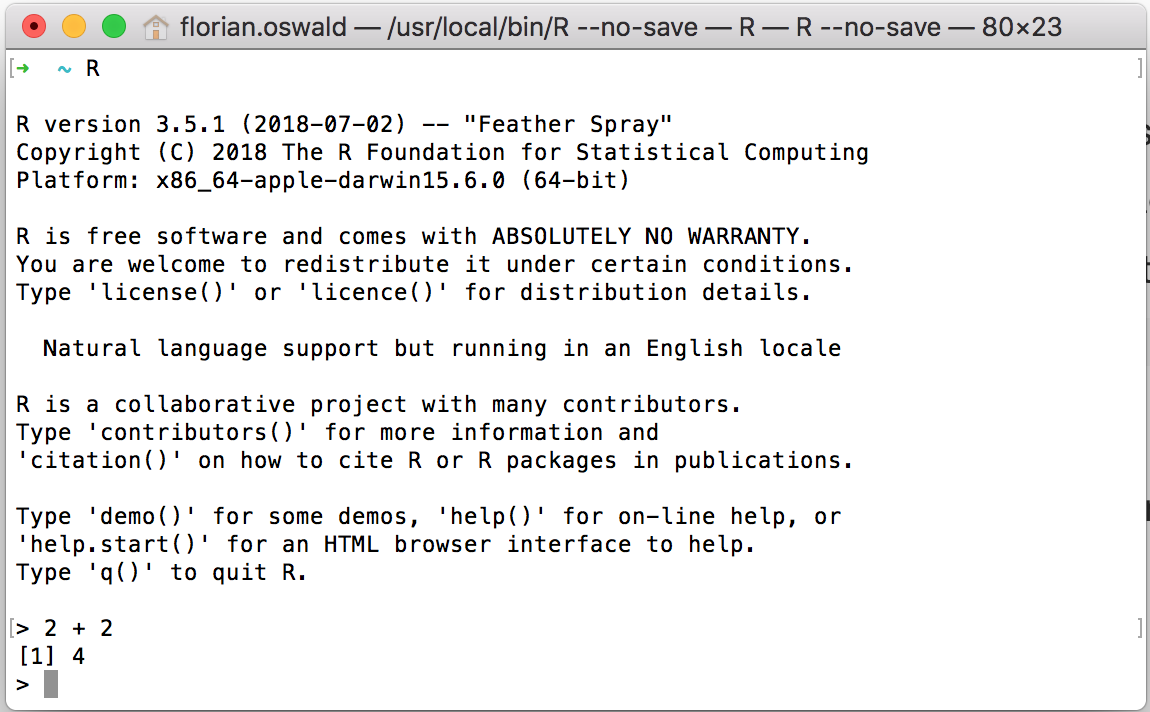
\includegraphics[width=0.5\linewidth]{images/console} 

}

\caption{R GUI symbol and R in a MacOS Terminal}\label{fig:console2}
\end{figure}

Typing one command after the other into the console is not very
convenient as our analysis becomes more involved. Ideally, we would like
to collect all command statements in a file and run them one after the
other, automatically. We can do this by writing so-called \textbf{script
files} or just \textbf{scripts}, i.e.~simple text files with extension
\texttt{.R} or \texttt{.r} which can be \emph{inserted} (or
\emph{sourced}) into an \texttt{R} session. RStudio makes this process
very easy.

Open \texttt{RStudio} by clicking on the \texttt{RStudio} application on
your computer, and notice how different the whole environment is from
the basic \texttt{R} console -- in fact, that \emph{very same}
\texttt{R} console is running in your bottom left panel. The upper-left
panel is a space for you to write scripts -- that is to say many lines
of codes which you can run when you choose to. To run a single line of
code, simply highlight it and hit \texttt{Command} + \texttt{Return}.

\begin{note}
We highly recommend that you use \texttt{RStudio} for everything related
to this course (in particular, to launch our apps and tutorials).
\end{note}

RStudio has a large number of useful keyboard shortcuts. A list of these
can be found using a keyboard shortcut -- the keyboard shortcut to rule
them all:

\begin{itemize}
\tightlist
\item
  On Windows: \texttt{Alt} + \texttt{Shift} + \texttt{K}
\item
  On Mac: \texttt{Option} + \texttt{Shift} + \texttt{K}
\end{itemize}

The \texttt{RStudio} team has developed
\href{https://www.rstudio.com/resources/cheatsheets/}{a number of
``cheatsheets''} for working with both \texttt{R} and \texttt{RStudio}.
\href{http://www.rstudio.com/wp-content/uploads/2016/05/base-r.pdf}{This
particular cheatseet for Base \texttt{R}} will summarize many of the
concepts in this document. \footnote{When programming, it is often a
  good practice to follow a style guide. (Where do spaces go? Tabs or
  spaces? Underscores or CamelCase when naming variables?) No style
  guide is ``correct'' but it helps to be aware of what others do. The
  more import thing is to be consistent within your own code. Here are
  two guides: \href{http://adv-r.had.co.nz/Style.html}{Hadley Wickham
  Style Guide}, and the
  \href{https://google.github.io/styleguide/Rguide.xml}{Google Style
  Guide}. For this course, our main deviation from these two guides is
  the use of \texttt{=} in place of \texttt{\textless{}-}. For all
  practical purposes, you should think \texttt{=} whenever you see
  \texttt{\textless{}-}.}

\subsection{First Glossary}\label{first-glossary}

\begin{itemize}
\tightlist
\item
  \texttt{R}: a statistical programming language
\item
  \texttt{RStudio}: an integrated development environment (IDE) to work
  with \texttt{R}
\item
  \emph{command}: user input (text or numbers) that \texttt{R}
  \emph{understands}.
\item
  \emph{script}: a list of commands collected in a text file, each
  separated by a new line, to be run one after the other.
\end{itemize}

\section{Basic Calculations}\label{basic-calculations}

To get started, we'll use \texttt{R} like a simple calculator. Run the
following code either directly from your RStudio console, or in RStudio
by writting them in a script and running them using \texttt{Command} +
\texttt{Return}.

\subsubsection*{Addition, Subtraction, Multiplication and
Division}\label{addition-subtraction-multiplication-and-division}
\addcontentsline{toc}{subsubsection}{Addition, Subtraction,
Multiplication and Division}

\begin{longtable}[]{@{}ccc@{}}
\toprule
Math & \texttt{R} code & Result\tabularnewline
\midrule
\endhead
\(3 + 2\) & \texttt{3\ +\ 2} & 5\tabularnewline
\(3 - 2\) & \texttt{3\ -\ 2} & 1\tabularnewline
\(3 \cdot2\) & \texttt{3\ *\ 2} & 6\tabularnewline
\(3 / 2\) & \texttt{3\ /\ 2} & 1.5\tabularnewline
\bottomrule
\end{longtable}

\subsubsection*{Exponents}\label{exponents}
\addcontentsline{toc}{subsubsection}{Exponents}

\begin{longtable}[]{@{}ccc@{}}
\toprule
Math & \texttt{R} code & Result\tabularnewline
\midrule
\endhead
\(3^2\) & \texttt{3\ \^{}\ 2} & 9\tabularnewline
\(2^{(-3)}\) & \texttt{2\ \^{}\ (-3)} & 0.125\tabularnewline
\(100^{1/2}\) & \texttt{100\ \^{}\ (1\ /\ 2)} & 10\tabularnewline
\(\sqrt{100}\) & \texttt{sqrt(100)} & 10\tabularnewline
\bottomrule
\end{longtable}

\subsubsection*{Mathematical Constants}\label{mathematical-constants}
\addcontentsline{toc}{subsubsection}{Mathematical Constants}

\begin{longtable}[]{@{}ccc@{}}
\toprule
Math & \texttt{R} code & Result\tabularnewline
\midrule
\endhead
\(\pi\) & \texttt{pi} & 3.1415927\tabularnewline
\(e\) & \texttt{exp(1)} & 2.7182818\tabularnewline
\bottomrule
\end{longtable}

\subsubsection*{Logarithms}\label{logarithms}
\addcontentsline{toc}{subsubsection}{Logarithms}

Note that we will use \(\ln\) and \(\log\) interchangeably to mean the
natural logarithm. There is no \texttt{ln()} in \texttt{R}, instead it
uses \texttt{log()} to mean the natural logarithm.

\begin{longtable}[]{@{}ccc@{}}
\toprule
Math & \texttt{R} code & Result\tabularnewline
\midrule
\endhead
\(\log(e)\) & \texttt{log(exp(1))} & 1\tabularnewline
\(\log_{10}(1000)\) & \texttt{log10(1000)} & 3\tabularnewline
\(\log_{2}(8)\) & \texttt{log2(8)} & 3\tabularnewline
\(\log_{4}(16)\) & \texttt{log(16,\ base\ =\ 4)} & 2\tabularnewline
\bottomrule
\end{longtable}

\subsubsection*{Trigonometry}\label{trigonometry}
\addcontentsline{toc}{subsubsection}{Trigonometry}

\begin{longtable}[]{@{}ccc@{}}
\toprule
Math & \texttt{R} code & Result\tabularnewline
\midrule
\endhead
\(\sin(\pi / 2)\) & \texttt{sin(pi\ /\ 2)} & 1\tabularnewline
\(\cos(0)\) & \texttt{cos(0)} & 1\tabularnewline
\bottomrule
\end{longtable}

\section{Getting Help}\label{getting-help}

In using \texttt{R} as a calculator, we have seen a number of functions:
\texttt{sqrt()}, \texttt{exp()}, \texttt{log()} and \texttt{sin()}. To
get documentation about a function in \texttt{R}, simply put a question
mark in front of the function name, or call the function
\texttt{help(function)} and RStudio will display the documentation, for
example:

\begin{Shaded}
\begin{Highlighting}[]
\NormalTok{?log}
\NormalTok{?sin}
\NormalTok{?paste}
\NormalTok{?lm}
\KeywordTok{help}\NormalTok{(lm)   }\CommentTok{# help() is equivalent}
\KeywordTok{help}\NormalTok{(ggplot,}\DataTypeTok{package=}\StringTok{"ggplot2"}\NormalTok{)  }\CommentTok{# show help from a certain package}
\end{Highlighting}
\end{Shaded}

Frequently one of the most difficult things to do when learning
\texttt{R} is asking for help. First, you need to decide to ask for
help, then you need to know \emph{how} to ask for help. Your very first
line of defense should be to Google your error message or a short
description of your issue. (The ability to solve problems using this
method is quickly becoming an extremely valuable skill.) If that fails,
and it eventually will, you should ask for help. There are a number of
things you should include when contacting an instructor, or posting to a
help website such as \href{https://stackoverflow.com}{Stack Overflow}.

\begin{itemize}
\tightlist
\item
  Describe what you expect the code to do.
\item
  State the end goal you are trying to achieve. (Sometimes what you
  expect the code to do, is not what you want to actually do.)
\item
  Provide the full text of any errors you have received.
\item
  Provide enough code to recreate the error. Often for the purpose of
  this course, you could simply post your entire \texttt{.R} script or
  \texttt{.Rmd} to \texttt{slack}.
\item
  Sometimes it is also helpful to include a screenshot of your entire
  RStudio window when the error occurs.
\end{itemize}

If you follow these steps, you will get your issue resolved much
quicker, and possibly learn more in the process. Do not be discouraged
by running into errors and difficulties when learning \texttt{R}. (Or
any other technical skill.) It is simply part of the learning process.

\section{Installing Packages}\label{installing-packages}

\texttt{R} comes with a number of built-in functions and datasets, but
one of the main strengths of \texttt{R} as an open-source project is its
package system. Packages add additional functions and data. Frequently
if you want to do something in \texttt{R}, and it is not available by
default, there is a good chance that there is a package that will
fulfill your needs.

To install a package, use the \texttt{install.packages()} function.
Think of this as buying a recipe book from the store, bringing it home,
and putting it on your shelf (i.e.~into your library):

\begin{Shaded}
\begin{Highlighting}[]
\KeywordTok{install.packages}\NormalTok{(}\StringTok{"ggplot2"}\NormalTok{)}
\end{Highlighting}
\end{Shaded}

Once a package is installed, it must be loaded into your current
\texttt{R} session before being used. Think of this as taking the book
off of the shelf and opening it up to read.

\begin{Shaded}
\begin{Highlighting}[]
\KeywordTok{library}\NormalTok{(ggplot2)}
\end{Highlighting}
\end{Shaded}

Once you close \texttt{R}, all the packages are closed and put back on
the imaginary shelf. The next time you open \texttt{R}, you do not have
to install the package again, but you do have to load any packages you
intend to use by invoking \texttt{library()}.

\section{\texorpdfstring{\texttt{Code} vs Output in this
Book}{Code vs Output in this Book}}\label{code-output}

A quick note on styling choices in this book. We had to make a decision
how to visually separate \texttt{R} code and resulting output in this
book. We decided to prefix all output lines with
\texttt{\#OUT\textgreater{}} to make the distinction. A typical code
snippet with output is thus going to look like this:

\begin{Shaded}
\begin{Highlighting}[]
\DecValTok{1} \OperatorTok{+}\StringTok{ }\DecValTok{3}
\end{Highlighting}
\end{Shaded}

\begin{verbatim}
#OUT> [1] 4
\end{verbatim}

\begin{Shaded}
\begin{Highlighting}[]
\CommentTok{# everything after a # is a comment, i.e. R disregards it.}
\end{Highlighting}
\end{Shaded}

where you see on the first line the \texttt{R} code, and on the second
line the output. As mentioned, that line starts with
\texttt{\#OUT\textgreater{}} to say \emph{this is an output}, followed
by \texttt{{[}1{]}} (indicating this is a vector of length \emph{one} -
more on this below!), followed by the actual result -
\texttt{1\ +\ 3\ =\ 4}!

Notice that you can simply copy and paste all the code you see into your
\texttt{R} console. In fact, you are \emph{strongly} encouraged to
actually do this and try out \textbf{all the code} you see in this book.

Finally, please note that this way of showing output is fully our choice
in this textbook, and that you should expect other output formats
elsewhere. For example, in my \texttt{RStudio} console, the above code
and output looks like this:

\begin{Shaded}
\begin{Highlighting}[]
\OperatorTok{>}\StringTok{ }\DecValTok{1} \OperatorTok{+}\StringTok{ }\DecValTok{3}
\NormalTok{[}\DecValTok{1}\NormalTok{] }\DecValTok{4}
\end{Highlighting}
\end{Shaded}

\section{\texorpdfstring{\texttt{ScPoEconometrics}
Package}{ScPoEconometrics Package}}\label{install-package}

To fully take advantage of our course, please install the associated
\texttt{R} package directly from its online code repository. You can do
this by copy and pasting the following three lines into your \texttt{R}
console:

\begin{Shaded}
\begin{Highlighting}[]
\ControlFlowTok{if}\NormalTok{ (}\OperatorTok{!}\KeywordTok{require}\NormalTok{(}\StringTok{"devtools"}\NormalTok{)) }\KeywordTok{install.packages}\NormalTok{(}\StringTok{"devtools"}\NormalTok{)}
\KeywordTok{library}\NormalTok{(devtools)}
\KeywordTok{install_github}\NormalTok{(}\DataTypeTok{repo =} \StringTok{"ScPoEcon/ScPoEconometrics"}\NormalTok{)}
\end{Highlighting}
\end{Shaded}

In order to check whether everything works fine, you could load the
library, and check it's current version:

\begin{Shaded}
\begin{Highlighting}[]
\KeywordTok{library}\NormalTok{(ScPoEconometrics)}
\KeywordTok{packageVersion}\NormalTok{(}\StringTok{"ScPoEconometrics"}\NormalTok{)}
\end{Highlighting}
\end{Shaded}

\begin{verbatim}
#OUT> [1] '0.2.6'
\end{verbatim}

\section{Data Types}\label{data-types}

\texttt{R} has a number of basic \emph{data types}. While \texttt{R} is
not a \emph{strongly typed language} (i.e.~you can be agnostic about
types most of the times), it is useful to know what data types are
available to you:

\begin{itemize}
\tightlist
\item
  Numeric

  \begin{itemize}
  \tightlist
  \item
    Also known as Double. The default type when dealing with numbers.
  \item
    Examples: \texttt{1}, \texttt{1.0}, \texttt{42.5}
  \end{itemize}
\item
  Integer

  \begin{itemize}
  \tightlist
  \item
    Examples: \texttt{1L}, \texttt{2L}, \texttt{42L}
  \end{itemize}
\item
  Complex

  \begin{itemize}
  \tightlist
  \item
    Example: \texttt{4\ +\ 2i}
  \end{itemize}
\item
  Logical

  \begin{itemize}
  \tightlist
  \item
    Two possible values: \texttt{TRUE} and \texttt{FALSE}
  \item
    You can also use \texttt{T} and \texttt{F}, but this is \emph{not}
    recommended.
  \item
    \texttt{NA} is also considered logical.
  \end{itemize}
\item
  Character

  \begin{itemize}
  \tightlist
  \item
    Examples: \texttt{"a"}, \texttt{"Statistics"},
    \texttt{"1\ plus\ 2."}
  \end{itemize}
\item
  Categorical or \texttt{factor}

  \begin{itemize}
  \tightlist
  \item
    A mixture of integer and character. A \texttt{factor} variable
    assigns a label to a numeric value.
  \item
    For example \texttt{factor(x=c(0,1),labels=c("male","female"))}
    assigns the string \emph{male} to the numeric values \texttt{0}, and
    the string \emph{female} to the value \texttt{1}.
  \end{itemize}
\end{itemize}

\section{Data Structures}\label{data-structures}

\texttt{R} also has a number of basic data \emph{structures}. A data
structure is either homogeneous (all elements are of the same data type)
or heterogeneous (elements can be of more than one data type).

\begin{longtable}[]{@{}ccc@{}}
\toprule
Dimension & \textbf{Homogeneous} & \textbf{Heterogeneous}\tabularnewline
\midrule
\endhead
1 & Vector & List\tabularnewline
2 & Matrix & Data Frame\tabularnewline
3+ & Array & nested Lists\tabularnewline
\bottomrule
\end{longtable}

\subsection{Vectors}\label{vectors}

Many operations in \texttt{R} make heavy use of \textbf{vectors}. A
vector is a \emph{container} for objects of identical type (see
\ref{data-types} above). Vectors in \texttt{R} are indexed starting at
\texttt{1}. That is what the \texttt{{[}1{]}} in the output is
indicating, that the first element of the row being displayed is the
first element of the vector. Larger vectors will start additional rows
with something like \texttt{{[}7{]}} where \texttt{7} is the index of
the first element of that row.

Possibly the most common way to create a vector in \texttt{R} is using
the \texttt{c()} function, which is short for ``combine''. As the name
suggests, it combines a list of elements separated by commas. (Are you
busy typing all of those examples into your \texttt{R} console? :-) )

\begin{Shaded}
\begin{Highlighting}[]
\KeywordTok{c}\NormalTok{(}\DecValTok{1}\NormalTok{, }\DecValTok{3}\NormalTok{, }\DecValTok{5}\NormalTok{, }\DecValTok{7}\NormalTok{, }\DecValTok{8}\NormalTok{, }\DecValTok{9}\NormalTok{)}
\end{Highlighting}
\end{Shaded}

\begin{verbatim}
#OUT> [1] 1 3 5 7 8 9
\end{verbatim}

Here \texttt{R} simply outputs this vector. If we would like to store
this vector in a \textbf{variable} we can do so with the
\textbf{assignment} operator \texttt{=}. In this case the variable
\texttt{x} now holds the vector we just created, and we can access the
vector by typing \texttt{x}.

\begin{Shaded}
\begin{Highlighting}[]
\NormalTok{x =}\StringTok{ }\KeywordTok{c}\NormalTok{(}\DecValTok{1}\NormalTok{, }\DecValTok{3}\NormalTok{, }\DecValTok{5}\NormalTok{, }\DecValTok{7}\NormalTok{, }\DecValTok{8}\NormalTok{, }\DecValTok{9}\NormalTok{)}
\NormalTok{x}
\end{Highlighting}
\end{Shaded}

\begin{verbatim}
#OUT> [1] 1 3 5 7 8 9
\end{verbatim}

As an aside, there is a long history of the assignment operator in
\texttt{R}, partially due to the keys available on the
\href{https://twitter.com/kwbroman/status/747829864091127809}{keyboards
of the creators of the \texttt{S} language.} (Which preceded
\texttt{R}.) For simplicity we will use \texttt{=}, but know that often
you will see \texttt{\textless{}-} as the assignment operator.

Because vectors must contain elements that are all the same type,
\texttt{R} will automatically \textbf{coerce} (i.e.~convert) to a single
type when attempting to create a vector that combines multiple types.

\begin{Shaded}
\begin{Highlighting}[]
\KeywordTok{c}\NormalTok{(}\DecValTok{42}\NormalTok{, }\StringTok{"Statistics"}\NormalTok{, }\OtherTok{TRUE}\NormalTok{)}
\end{Highlighting}
\end{Shaded}

\begin{verbatim}
#OUT> [1] "42"         "Statistics" "TRUE"
\end{verbatim}

\begin{Shaded}
\begin{Highlighting}[]
\KeywordTok{c}\NormalTok{(}\DecValTok{42}\NormalTok{, }\OtherTok{TRUE}\NormalTok{)}
\end{Highlighting}
\end{Shaded}

\begin{verbatim}
#OUT> [1] 42  1
\end{verbatim}

Frequently you may wish to create a vector based on a sequence of
numbers. The quickest and easiest way to do this is with the \texttt{:}
operator, which creates a sequence of integers between two specified
integers.

\begin{Shaded}
\begin{Highlighting}[]
\NormalTok{(}\DataTypeTok{y =} \DecValTok{1}\OperatorTok{:}\DecValTok{100}\NormalTok{)}
\end{Highlighting}
\end{Shaded}

\begin{verbatim}
#OUT>   [1]   1   2   3   4   5   6   7   8   9  10  11  12  13  14  15  16  17  18
#OUT>  [19]  19  20  21  22  23  24  25  26  27  28  29  30  31  32  33  34  35  36
#OUT>  [37]  37  38  39  40  41  42  43  44  45  46  47  48  49  50  51  52  53  54
#OUT>  [55]  55  56  57  58  59  60  61  62  63  64  65  66  67  68  69  70  71  72
#OUT>  [73]  73  74  75  76  77  78  79  80  81  82  83  84  85  86  87  88  89  90
#OUT>  [91]  91  92  93  94  95  96  97  98  99 100
\end{verbatim}

Here we see \texttt{R} labeling the rows after the first since this is a
large vector. Also, we see that by putting parentheses around the
assignment, \texttt{R} both stores the vector in a variable called
\texttt{y} and automatically outputs \texttt{y} to the console.

Note that scalars do not exists in \texttt{R}. They are simply vectors
of length \texttt{1}.

\begin{Shaded}
\begin{Highlighting}[]
\DecValTok{2}
\end{Highlighting}
\end{Shaded}

\begin{verbatim}
#OUT> [1] 2
\end{verbatim}

If we want to create a sequence that isn't limited to integers and
increasing by 1 at a time, we can use the \texttt{seq()} function.

\begin{Shaded}
\begin{Highlighting}[]
\KeywordTok{seq}\NormalTok{(}\DataTypeTok{from =} \FloatTok{1.5}\NormalTok{, }\DataTypeTok{to =} \FloatTok{4.2}\NormalTok{, }\DataTypeTok{by =} \FloatTok{0.1}\NormalTok{)}
\end{Highlighting}
\end{Shaded}

\begin{verbatim}
#OUT>  [1] 1.5 1.6 1.7 1.8 1.9 2.0 2.1 2.2 2.3 2.4 2.5 2.6 2.7 2.8 2.9 3.0 3.1 3.2 3.3
#OUT> [20] 3.4 3.5 3.6 3.7 3.8 3.9 4.0 4.1 4.2
\end{verbatim}

We will discuss functions in detail later, but note here that the input
labels \texttt{from}, \texttt{to}, and \texttt{by} are optional.

\begin{Shaded}
\begin{Highlighting}[]
\KeywordTok{seq}\NormalTok{(}\FloatTok{1.5}\NormalTok{, }\FloatTok{4.2}\NormalTok{, }\FloatTok{0.1}\NormalTok{)}
\end{Highlighting}
\end{Shaded}

\begin{verbatim}
#OUT>  [1] 1.5 1.6 1.7 1.8 1.9 2.0 2.1 2.2 2.3 2.4 2.5 2.6 2.7 2.8 2.9 3.0 3.1 3.2 3.3
#OUT> [20] 3.4 3.5 3.6 3.7 3.8 3.9 4.0 4.1 4.2
\end{verbatim}

Another common operation to create a vector is \texttt{rep()}, which can
repeat a single value a number of times.

\begin{Shaded}
\begin{Highlighting}[]
\KeywordTok{rep}\NormalTok{(}\StringTok{"A"}\NormalTok{, }\DataTypeTok{times =} \DecValTok{10}\NormalTok{)}
\end{Highlighting}
\end{Shaded}

\begin{verbatim}
#OUT>  [1] "A" "A" "A" "A" "A" "A" "A" "A" "A" "A"
\end{verbatim}

The \texttt{rep()} function can be used to repeat a vector some number
of times.

\begin{Shaded}
\begin{Highlighting}[]
\KeywordTok{rep}\NormalTok{(x, }\DataTypeTok{times =} \DecValTok{3}\NormalTok{)}
\end{Highlighting}
\end{Shaded}

\begin{verbatim}
#OUT>  [1] 1 3 5 7 8 9 1 3 5 7 8 9 1 3 5 7 8 9
\end{verbatim}

We have now seen four different ways to create vectors:

\begin{itemize}
\tightlist
\item
  \texttt{c()}
\item
  \texttt{:}
\item
  \texttt{seq()}
\item
  \texttt{rep()}
\end{itemize}

So far we have mostly used them in isolation, but they are often used
together.

\begin{Shaded}
\begin{Highlighting}[]
\KeywordTok{c}\NormalTok{(x, }\KeywordTok{rep}\NormalTok{(}\KeywordTok{seq}\NormalTok{(}\DecValTok{1}\NormalTok{, }\DecValTok{9}\NormalTok{, }\DecValTok{2}\NormalTok{), }\DecValTok{3}\NormalTok{), }\KeywordTok{c}\NormalTok{(}\DecValTok{1}\NormalTok{, }\DecValTok{2}\NormalTok{, }\DecValTok{3}\NormalTok{), }\DecValTok{42}\NormalTok{, }\DecValTok{2}\OperatorTok{:}\DecValTok{4}\NormalTok{)}
\end{Highlighting}
\end{Shaded}

\begin{verbatim}
#OUT>  [1]  1  3  5  7  8  9  1  3  5  7  9  1  3  5  7  9  1  3  5  7  9  1  2  3 42
#OUT> [26]  2  3  4
\end{verbatim}

The length of a vector can be obtained with the \texttt{length()}
function.

\begin{Shaded}
\begin{Highlighting}[]
\KeywordTok{length}\NormalTok{(x)}
\end{Highlighting}
\end{Shaded}

\begin{verbatim}
#OUT> [1] 6
\end{verbatim}

\begin{Shaded}
\begin{Highlighting}[]
\KeywordTok{length}\NormalTok{(y)}
\end{Highlighting}
\end{Shaded}

\begin{verbatim}
#OUT> [1] 100
\end{verbatim}

\begin{warning}
Let's try this out! \textbf{Your turn}:
\end{warning}

\subsubsection{Task 1}\label{task-1}

\begin{enumerate}
\def\labelenumi{\arabic{enumi}.}
\tightlist
\item
  Create a vector of five ones, i.e. \texttt{{[}1,1,1,1,1{]}}
\item
  Notice that the colon operator \texttt{a:b} is just short for
  \emph{construct a sequence \textbf{from} \texttt{a} \textbf{to}
  \texttt{b}}. Create a vector the counts down from 10 to 0, i.e.~it
  looks like \texttt{{[}10,9,8,7,6,5,4,3,2,1,0{]}}!
\item
  the \texttt{rep} function takes additional arguments \texttt{times}
  (as above), and \texttt{each}, which tells you how often \emph{each
  element} should be repeated (as opposed to the entire input vector).
  Use \texttt{rep} to create a vector that looks like this:
  \texttt{{[}1\ 1\ 1\ 2\ 2\ 2\ 3\ 3\ 3\ 1\ 1\ 1\ 2\ 2\ 2\ 3\ 3\ 3{]}}
\end{enumerate}

\subsubsection{Subsetting}\label{subsetting}

To subset a vector, i.e.~to choose only some elements of it, we use
square brackets, \texttt{{[}{]}}. Here we see that \texttt{x{[}1{]}}
returns the first element, and \texttt{x{[}3{]}} returns the third
element:

\begin{Shaded}
\begin{Highlighting}[]
\NormalTok{x}
\end{Highlighting}
\end{Shaded}

\begin{verbatim}
#OUT> [1] 1 3 5 7 8 9
\end{verbatim}

\begin{Shaded}
\begin{Highlighting}[]
\NormalTok{x[}\DecValTok{1}\NormalTok{]}
\end{Highlighting}
\end{Shaded}

\begin{verbatim}
#OUT> [1] 1
\end{verbatim}

\begin{Shaded}
\begin{Highlighting}[]
\NormalTok{x[}\DecValTok{3}\NormalTok{]}
\end{Highlighting}
\end{Shaded}

\begin{verbatim}
#OUT> [1] 5
\end{verbatim}

We can also exclude certain indexes, in this case the second element.

\begin{Shaded}
\begin{Highlighting}[]
\NormalTok{x[}\OperatorTok{-}\DecValTok{2}\NormalTok{]}
\end{Highlighting}
\end{Shaded}

\begin{verbatim}
#OUT> [1] 1 5 7 8 9
\end{verbatim}

Lastly we see that we can subset based on a vector of indices.

\begin{Shaded}
\begin{Highlighting}[]
\NormalTok{x[}\DecValTok{1}\OperatorTok{:}\DecValTok{3}\NormalTok{]}
\end{Highlighting}
\end{Shaded}

\begin{verbatim}
#OUT> [1] 1 3 5
\end{verbatim}

\begin{Shaded}
\begin{Highlighting}[]
\NormalTok{x[}\KeywordTok{c}\NormalTok{(}\DecValTok{1}\NormalTok{,}\DecValTok{3}\NormalTok{,}\DecValTok{4}\NormalTok{)]}
\end{Highlighting}
\end{Shaded}

\begin{verbatim}
#OUT> [1] 1 5 7
\end{verbatim}

All of the above are subsetting a vector using a vector of indexes.
(Remember a single number is still a vector.) We could instead use a
vector of logical values.

\begin{Shaded}
\begin{Highlighting}[]
\NormalTok{z =}\StringTok{ }\KeywordTok{c}\NormalTok{(}\OtherTok{TRUE}\NormalTok{, }\OtherTok{TRUE}\NormalTok{, }\OtherTok{FALSE}\NormalTok{, }\OtherTok{TRUE}\NormalTok{, }\OtherTok{TRUE}\NormalTok{, }\OtherTok{FALSE}\NormalTok{)}
\NormalTok{z}
\end{Highlighting}
\end{Shaded}

\begin{verbatim}
#OUT> [1]  TRUE  TRUE FALSE  TRUE  TRUE FALSE
\end{verbatim}

\begin{Shaded}
\begin{Highlighting}[]
\NormalTok{x[z]}
\end{Highlighting}
\end{Shaded}

\begin{verbatim}
#OUT> [1] 1 3 7 8
\end{verbatim}

\texttt{R} is able to perform many operations on vectors and scalars
alike:

\begin{Shaded}
\begin{Highlighting}[]
\NormalTok{x =}\StringTok{ }\DecValTok{1}\OperatorTok{:}\DecValTok{10}  \CommentTok{# a vector}
\NormalTok{x }\OperatorTok{+}\StringTok{ }\DecValTok{1}     \CommentTok{# add a scalar}
\end{Highlighting}
\end{Shaded}

\begin{verbatim}
#OUT>  [1]  2  3  4  5  6  7  8  9 10 11
\end{verbatim}

\begin{Shaded}
\begin{Highlighting}[]
\DecValTok{2} \OperatorTok{*}\StringTok{ }\NormalTok{x     }\CommentTok{# multiply all elements by 2}
\end{Highlighting}
\end{Shaded}

\begin{verbatim}
#OUT>  [1]  2  4  6  8 10 12 14 16 18 20
\end{verbatim}

\begin{Shaded}
\begin{Highlighting}[]
\DecValTok{2} \OperatorTok{^}\StringTok{ }\NormalTok{x     }\CommentTok{# take 2 to the x as exponents}
\end{Highlighting}
\end{Shaded}

\begin{verbatim}
#OUT>  [1]    2    4    8   16   32   64  128  256  512 1024
\end{verbatim}

\begin{Shaded}
\begin{Highlighting}[]
\KeywordTok{sqrt}\NormalTok{(x)   }\CommentTok{# compute the square root of all elements in x}
\end{Highlighting}
\end{Shaded}

\begin{verbatim}
#OUT>  [1] 1.000000 1.414214 1.732051 2.000000 2.236068 2.449490 2.645751 2.828427
#OUT>  [9] 3.000000 3.162278
\end{verbatim}

\begin{Shaded}
\begin{Highlighting}[]
\KeywordTok{log}\NormalTok{(x)    }\CommentTok{# take the natural log of all elements in x}
\end{Highlighting}
\end{Shaded}

\begin{verbatim}
#OUT>  [1] 0.0000000 0.6931472 1.0986123 1.3862944 1.6094379 1.7917595 1.9459101
#OUT>  [8] 2.0794415 2.1972246 2.3025851
\end{verbatim}

\begin{Shaded}
\begin{Highlighting}[]
\NormalTok{x }\OperatorTok{+}\StringTok{ }\DecValTok{2}\OperatorTok{*}\NormalTok{x   }\CommentTok{# add vector x to vector 2x}
\end{Highlighting}
\end{Shaded}

\begin{verbatim}
#OUT>  [1]  3  6  9 12 15 18 21 24 27 30
\end{verbatim}

We see that when a function like \texttt{log()} is called on a vector
\texttt{x}, a vector is returned which has applied the function to each
element of the vector \texttt{x}.

\subsection{Logical Operators}\label{logical-operators}

\begin{longtable}[]{@{}lccc@{}}
\toprule
Operator & Summary & Example & Result\tabularnewline
\midrule
\endhead
\texttt{x\ \textless{}\ y} & \texttt{x} less than \texttt{y} &
\texttt{3\ \textless{}\ 42} & TRUE\tabularnewline
\texttt{x\ \textgreater{}\ y} & \texttt{x} greater than \texttt{y} &
\texttt{3\ \textgreater{}\ 42} & FALSE\tabularnewline
\texttt{x\ \textless{}=\ y} & \texttt{x} less than or equal to
\texttt{y} & \texttt{3\ \textless{}=\ 42} & TRUE\tabularnewline
\texttt{x\ \textgreater{}=\ y} & \texttt{x} greater than or equal to
\texttt{y} & \texttt{3\ \textgreater{}=\ 42} & FALSE\tabularnewline
\texttt{x\ ==\ y} & \texttt{x}equal to \texttt{y} & \texttt{3\ ==\ 42} &
FALSE\tabularnewline
\texttt{x\ !=\ y} & \texttt{x} not equal to \texttt{y} &
\texttt{3\ !=\ 42} & TRUE\tabularnewline
\texttt{!x} & not \texttt{x} & \texttt{!(3\ \textgreater{}\ 42)} &
TRUE\tabularnewline
\texttt{x\ \textbar{}\ y} & \texttt{x} or \texttt{y} &
\texttt{(3\ \textgreater{}\ 42)\ \textbar{}\ TRUE} & TRUE\tabularnewline
\texttt{x\ \&\ y} & \texttt{x} and \texttt{y} &
\texttt{(3\ \textless{}\ 4)\ \&\ (\ 42\ \textgreater{}\ 13)} &
TRUE\tabularnewline
\bottomrule
\end{longtable}

In \texttt{R}, logical operators also work on vectors:

\begin{Shaded}
\begin{Highlighting}[]
\NormalTok{x =}\StringTok{ }\KeywordTok{c}\NormalTok{(}\DecValTok{1}\NormalTok{, }\DecValTok{3}\NormalTok{, }\DecValTok{5}\NormalTok{, }\DecValTok{7}\NormalTok{, }\DecValTok{8}\NormalTok{, }\DecValTok{9}\NormalTok{)}
\end{Highlighting}
\end{Shaded}

\begin{Shaded}
\begin{Highlighting}[]
\NormalTok{x }\OperatorTok{>}\StringTok{ }\DecValTok{3}
\end{Highlighting}
\end{Shaded}

\begin{verbatim}
#OUT> [1] FALSE FALSE  TRUE  TRUE  TRUE  TRUE
\end{verbatim}

\begin{Shaded}
\begin{Highlighting}[]
\NormalTok{x }\OperatorTok{<}\StringTok{ }\DecValTok{3}
\end{Highlighting}
\end{Shaded}

\begin{verbatim}
#OUT> [1]  TRUE FALSE FALSE FALSE FALSE FALSE
\end{verbatim}

\begin{Shaded}
\begin{Highlighting}[]
\NormalTok{x }\OperatorTok{==}\StringTok{ }\DecValTok{3}
\end{Highlighting}
\end{Shaded}

\begin{verbatim}
#OUT> [1] FALSE  TRUE FALSE FALSE FALSE FALSE
\end{verbatim}

\begin{Shaded}
\begin{Highlighting}[]
\NormalTok{x }\OperatorTok{!=}\StringTok{ }\DecValTok{3}
\end{Highlighting}
\end{Shaded}

\begin{verbatim}
#OUT> [1]  TRUE FALSE  TRUE  TRUE  TRUE  TRUE
\end{verbatim}

\begin{Shaded}
\begin{Highlighting}[]
\NormalTok{x }\OperatorTok{==}\StringTok{ }\DecValTok{3} \OperatorTok{&}\StringTok{ }\NormalTok{x }\OperatorTok{!=}\StringTok{ }\DecValTok{3}
\end{Highlighting}
\end{Shaded}

\begin{verbatim}
#OUT> [1] FALSE FALSE FALSE FALSE FALSE FALSE
\end{verbatim}

\begin{Shaded}
\begin{Highlighting}[]
\NormalTok{x }\OperatorTok{==}\StringTok{ }\DecValTok{3} \OperatorTok{|}\StringTok{ }\NormalTok{x }\OperatorTok{!=}\StringTok{ }\DecValTok{3}
\end{Highlighting}
\end{Shaded}

\begin{verbatim}
#OUT> [1] TRUE TRUE TRUE TRUE TRUE TRUE
\end{verbatim}

This is quite useful for subsetting.

\begin{Shaded}
\begin{Highlighting}[]
\NormalTok{x[x }\OperatorTok{>}\StringTok{ }\DecValTok{3}\NormalTok{]}
\end{Highlighting}
\end{Shaded}

\begin{verbatim}
#OUT> [1] 5 7 8 9
\end{verbatim}

\begin{Shaded}
\begin{Highlighting}[]
\NormalTok{x[x }\OperatorTok{!=}\StringTok{ }\DecValTok{3}\NormalTok{]}
\end{Highlighting}
\end{Shaded}

\begin{verbatim}
#OUT> [1] 1 5 7 8 9
\end{verbatim}

\begin{Shaded}
\begin{Highlighting}[]
\KeywordTok{sum}\NormalTok{(x }\OperatorTok{>}\StringTok{ }\DecValTok{3}\NormalTok{)}
\end{Highlighting}
\end{Shaded}

\begin{verbatim}
#OUT> [1] 4
\end{verbatim}

\begin{Shaded}
\begin{Highlighting}[]
\KeywordTok{as.numeric}\NormalTok{(x }\OperatorTok{>}\StringTok{ }\DecValTok{3}\NormalTok{)}
\end{Highlighting}
\end{Shaded}

\begin{verbatim}
#OUT> [1] 0 0 1 1 1 1
\end{verbatim}

Here we saw that using the \texttt{sum()} function on a vector of
logical \texttt{TRUE} and \texttt{FALSE} values that is the result of
\texttt{x\ \textgreater{}\ 3} results in a numeric result: you just
\emph{counted} for how many elements of \texttt{x}, the condition
\texttt{\textgreater{}\ 3} is \texttt{TRUE}. During the call to
\texttt{sum()}, \texttt{R} is first automatically coercing the logical
to numeric where \texttt{TRUE} is \texttt{1} and \texttt{FALSE} is
\texttt{0}. This coercion from logical to numeric happens for most
mathematical operations.

\begin{Shaded}
\begin{Highlighting}[]
\CommentTok{# which(condition of x) returns true/false  }
\CommentTok{# each index of x where condition is true}
\KeywordTok{which}\NormalTok{(x }\OperatorTok{>}\StringTok{ }\DecValTok{3}\NormalTok{)}
\end{Highlighting}
\end{Shaded}

\begin{verbatim}
#OUT> [1] 3 4 5 6
\end{verbatim}

\begin{Shaded}
\begin{Highlighting}[]
\NormalTok{x[}\KeywordTok{which}\NormalTok{(x }\OperatorTok{>}\StringTok{ }\DecValTok{3}\NormalTok{)]}
\end{Highlighting}
\end{Shaded}

\begin{verbatim}
#OUT> [1] 5 7 8 9
\end{verbatim}

\begin{Shaded}
\begin{Highlighting}[]
\KeywordTok{max}\NormalTok{(x)}
\end{Highlighting}
\end{Shaded}

\begin{verbatim}
#OUT> [1] 9
\end{verbatim}

\begin{Shaded}
\begin{Highlighting}[]
\KeywordTok{which}\NormalTok{(x }\OperatorTok{==}\StringTok{ }\KeywordTok{max}\NormalTok{(x))}
\end{Highlighting}
\end{Shaded}

\begin{verbatim}
#OUT> [1] 6
\end{verbatim}

\begin{Shaded}
\begin{Highlighting}[]
\KeywordTok{which.max}\NormalTok{(x)}
\end{Highlighting}
\end{Shaded}

\begin{verbatim}
#OUT> [1] 6
\end{verbatim}

\subsubsection{Task 2}\label{task-2}

\begin{enumerate}
\def\labelenumi{\arabic{enumi}.}
\tightlist
\item
  Create a vector filled with 10 numbers drawn from the uniform
  distribution (hint: use function \texttt{runif}) and store them in
  \texttt{x}.
\item
  Using logical subsetting as above, get all the elements of \texttt{x}
  which are larger than 0.5, and store them in \texttt{y}.
\item
  using the function \texttt{which}, store the \emph{indices} of all the
  elements of \texttt{x} which are larger than 0.5 in \texttt{iy}.
\item
  Check that \texttt{y} and \texttt{x{[}iy{]}} are identical.
\end{enumerate}

\subsection{Matrices}\label{matrices}

\texttt{R} can also be used for \textbf{matrix} calculations. Matrices
have rows and columns containing a single data type. In a matrix, the
order of rows and columns is important. (This is not true of \emph{data
frames}, which we will see later.)

Matrices can be created using the \texttt{matrix} function.

\begin{Shaded}
\begin{Highlighting}[]
\NormalTok{x =}\StringTok{ }\DecValTok{1}\OperatorTok{:}\DecValTok{9}
\NormalTok{x}
\end{Highlighting}
\end{Shaded}

\begin{verbatim}
#OUT> [1] 1 2 3 4 5 6 7 8 9
\end{verbatim}

\begin{Shaded}
\begin{Highlighting}[]
\NormalTok{X =}\StringTok{ }\KeywordTok{matrix}\NormalTok{(x, }\DataTypeTok{nrow =} \DecValTok{3}\NormalTok{, }\DataTypeTok{ncol =} \DecValTok{3}\NormalTok{)}
\NormalTok{X}
\end{Highlighting}
\end{Shaded}

\begin{verbatim}
#OUT>      [,1] [,2] [,3]
#OUT> [1,]    1    4    7
#OUT> [2,]    2    5    8
#OUT> [3,]    3    6    9
\end{verbatim}

Notice here that \texttt{R} is case sensitive (\texttt{x} vs
\texttt{X}).

By default the \texttt{matrix} function fills your data into the matrix
column by column. But we can also tell \texttt{R} to fill rows instead:

\begin{Shaded}
\begin{Highlighting}[]
\NormalTok{Y =}\StringTok{ }\KeywordTok{matrix}\NormalTok{(x, }\DataTypeTok{nrow =} \DecValTok{3}\NormalTok{, }\DataTypeTok{ncol =} \DecValTok{3}\NormalTok{, }\DataTypeTok{byrow =} \OtherTok{TRUE}\NormalTok{)}
\NormalTok{Y}
\end{Highlighting}
\end{Shaded}

\begin{verbatim}
#OUT>      [,1] [,2] [,3]
#OUT> [1,]    1    2    3
#OUT> [2,]    4    5    6
#OUT> [3,]    7    8    9
\end{verbatim}

We can also create a matrix of a specified dimension where every element
is the same, in this case \texttt{0}.

\begin{Shaded}
\begin{Highlighting}[]
\NormalTok{Z =}\StringTok{ }\KeywordTok{matrix}\NormalTok{(}\DecValTok{0}\NormalTok{, }\DecValTok{2}\NormalTok{, }\DecValTok{4}\NormalTok{)}
\NormalTok{Z}
\end{Highlighting}
\end{Shaded}

\begin{verbatim}
#OUT>      [,1] [,2] [,3] [,4]
#OUT> [1,]    0    0    0    0
#OUT> [2,]    0    0    0    0
\end{verbatim}

Like vectors, matrices can be subsetted using square brackets,
\texttt{{[}{]}}. However, since matrices are two-dimensional, we need to
specify both a row and a column when subsetting.

\begin{Shaded}
\begin{Highlighting}[]
\NormalTok{X}
\end{Highlighting}
\end{Shaded}

\begin{verbatim}
#OUT>      [,1] [,2] [,3]
#OUT> [1,]    1    4    7
#OUT> [2,]    2    5    8
#OUT> [3,]    3    6    9
\end{verbatim}

\begin{Shaded}
\begin{Highlighting}[]
\NormalTok{X[}\DecValTok{1}\NormalTok{, }\DecValTok{2}\NormalTok{]}
\end{Highlighting}
\end{Shaded}

\begin{verbatim}
#OUT> [1] 4
\end{verbatim}

Here we accessed the element in the first row and the second column. We
could also subset an entire row or column.

\begin{Shaded}
\begin{Highlighting}[]
\NormalTok{X[}\DecValTok{1}\NormalTok{, ]}
\end{Highlighting}
\end{Shaded}

\begin{verbatim}
#OUT> [1] 1 4 7
\end{verbatim}

\begin{Shaded}
\begin{Highlighting}[]
\NormalTok{X[, }\DecValTok{2}\NormalTok{]}
\end{Highlighting}
\end{Shaded}

\begin{verbatim}
#OUT> [1] 4 5 6
\end{verbatim}

We can also use vectors to subset more than one row or column at a time.
Here we subset to the first and third column of the second row:

\begin{Shaded}
\begin{Highlighting}[]
\NormalTok{X[}\DecValTok{2}\NormalTok{, }\KeywordTok{c}\NormalTok{(}\DecValTok{1}\NormalTok{, }\DecValTok{3}\NormalTok{)]}
\end{Highlighting}
\end{Shaded}

\begin{verbatim}
#OUT> [1] 2 8
\end{verbatim}

Matrices can also be created by combining vectors as columns, using
\texttt{cbind}, or combining vectors as rows, using \texttt{rbind}.

\begin{Shaded}
\begin{Highlighting}[]
\NormalTok{x =}\StringTok{ }\DecValTok{1}\OperatorTok{:}\DecValTok{9}
\KeywordTok{rev}\NormalTok{(x)}
\end{Highlighting}
\end{Shaded}

\begin{verbatim}
#OUT> [1] 9 8 7 6 5 4 3 2 1
\end{verbatim}

\begin{Shaded}
\begin{Highlighting}[]
\KeywordTok{rep}\NormalTok{(}\DecValTok{1}\NormalTok{, }\DecValTok{9}\NormalTok{)}
\end{Highlighting}
\end{Shaded}

\begin{verbatim}
#OUT> [1] 1 1 1 1 1 1 1 1 1
\end{verbatim}

\begin{Shaded}
\begin{Highlighting}[]
\KeywordTok{rbind}\NormalTok{(x, }\KeywordTok{rev}\NormalTok{(x), }\KeywordTok{rep}\NormalTok{(}\DecValTok{1}\NormalTok{, }\DecValTok{9}\NormalTok{))}
\end{Highlighting}
\end{Shaded}

\begin{verbatim}
#OUT>   [,1] [,2] [,3] [,4] [,5] [,6] [,7] [,8] [,9]
#OUT> x    1    2    3    4    5    6    7    8    9
#OUT>      9    8    7    6    5    4    3    2    1
#OUT>      1    1    1    1    1    1    1    1    1
\end{verbatim}

\begin{Shaded}
\begin{Highlighting}[]
\KeywordTok{cbind}\NormalTok{(}\DataTypeTok{col_1 =}\NormalTok{ x, }\DataTypeTok{col_2 =} \KeywordTok{rev}\NormalTok{(x), }\DataTypeTok{col_3 =} \KeywordTok{rep}\NormalTok{(}\DecValTok{1}\NormalTok{, }\DecValTok{9}\NormalTok{))}
\end{Highlighting}
\end{Shaded}

\begin{verbatim}
#OUT>       col_1 col_2 col_3
#OUT>  [1,]     1     9     1
#OUT>  [2,]     2     8     1
#OUT>  [3,]     3     7     1
#OUT>  [4,]     4     6     1
#OUT>  [5,]     5     5     1
#OUT>  [6,]     6     4     1
#OUT>  [7,]     7     3     1
#OUT>  [8,]     8     2     1
#OUT>  [9,]     9     1     1
\end{verbatim}

When using \texttt{rbind} and \texttt{cbind} you can specify
``argument'' names that will be used as column names.

\texttt{R} can then be used to perform matrix calculations.

\begin{Shaded}
\begin{Highlighting}[]
\NormalTok{x =}\StringTok{ }\DecValTok{1}\OperatorTok{:}\DecValTok{9}
\NormalTok{y =}\StringTok{ }\DecValTok{9}\OperatorTok{:}\DecValTok{1}
\NormalTok{X =}\StringTok{ }\KeywordTok{matrix}\NormalTok{(x, }\DecValTok{3}\NormalTok{, }\DecValTok{3}\NormalTok{)}
\NormalTok{Y =}\StringTok{ }\KeywordTok{matrix}\NormalTok{(y, }\DecValTok{3}\NormalTok{, }\DecValTok{3}\NormalTok{)}
\NormalTok{X}
\end{Highlighting}
\end{Shaded}

\begin{verbatim}
#OUT>      [,1] [,2] [,3]
#OUT> [1,]    1    4    7
#OUT> [2,]    2    5    8
#OUT> [3,]    3    6    9
\end{verbatim}

\begin{Shaded}
\begin{Highlighting}[]
\NormalTok{Y}
\end{Highlighting}
\end{Shaded}

\begin{verbatim}
#OUT>      [,1] [,2] [,3]
#OUT> [1,]    9    6    3
#OUT> [2,]    8    5    2
#OUT> [3,]    7    4    1
\end{verbatim}

\begin{Shaded}
\begin{Highlighting}[]
\NormalTok{X }\OperatorTok{+}\StringTok{ }\NormalTok{Y}
\end{Highlighting}
\end{Shaded}

\begin{verbatim}
#OUT>      [,1] [,2] [,3]
#OUT> [1,]   10   10   10
#OUT> [2,]   10   10   10
#OUT> [3,]   10   10   10
\end{verbatim}

\begin{Shaded}
\begin{Highlighting}[]
\NormalTok{X }\OperatorTok{-}\StringTok{ }\NormalTok{Y}
\end{Highlighting}
\end{Shaded}

\begin{verbatim}
#OUT>      [,1] [,2] [,3]
#OUT> [1,]   -8   -2    4
#OUT> [2,]   -6    0    6
#OUT> [3,]   -4    2    8
\end{verbatim}

\begin{Shaded}
\begin{Highlighting}[]
\NormalTok{X }\OperatorTok{*}\StringTok{ }\NormalTok{Y}
\end{Highlighting}
\end{Shaded}

\begin{verbatim}
#OUT>      [,1] [,2] [,3]
#OUT> [1,]    9   24   21
#OUT> [2,]   16   25   16
#OUT> [3,]   21   24    9
\end{verbatim}

\begin{Shaded}
\begin{Highlighting}[]
\NormalTok{X }\OperatorTok{/}\StringTok{ }\NormalTok{Y}
\end{Highlighting}
\end{Shaded}

\begin{verbatim}
#OUT>           [,1]      [,2]     [,3]
#OUT> [1,] 0.1111111 0.6666667 2.333333
#OUT> [2,] 0.2500000 1.0000000 4.000000
#OUT> [3,] 0.4285714 1.5000000 9.000000
\end{verbatim}

Note that \texttt{X\ *\ Y} is \textbf{not} matrix multiplication. It is
\emph{element by element} multiplication. (Same for \texttt{X\ /\ Y}).
Matrix multiplication uses \texttt{\%*\%}. Other matrix functions
include \texttt{t()} which gives the transpose of a matrix and
\texttt{solve()} which returns the inverse of a square matrix if it is
invertible.

\begin{Shaded}
\begin{Highlighting}[]
\NormalTok{X }\OperatorTok\StringTok{ }\NormalTok{Y}
\end{Highlighting}
\end{Shaded}

\begin{verbatim}
#OUT>      [,1] [,2] [,3]
#OUT> [1,]   90   54   18
#OUT> [2,]  114   69   24
#OUT> [3,]  138   84   30
\end{verbatim}

\begin{Shaded}
\begin{Highlighting}[]
\KeywordTok{t}\NormalTok{(X)}
\end{Highlighting}
\end{Shaded}

\begin{verbatim}
#OUT>      [,1] [,2] [,3]
#OUT> [1,]    1    2    3
#OUT> [2,]    4    5    6
#OUT> [3,]    7    8    9
\end{verbatim}

\subsection{Arrays}\label{arrays}

A vector is a one-dimensional array. A matrix is a two-dimensional
array. In \texttt{R} you can create arrays of arbitrary dimensionality
\texttt{N}. Here is how:

\begin{Shaded}
\begin{Highlighting}[]
\NormalTok{d =}\StringTok{ }\DecValTok{1}\OperatorTok{:}\DecValTok{16}
\NormalTok{d3 =}\StringTok{ }\KeywordTok{array}\NormalTok{(}\DataTypeTok{data =}\NormalTok{ d,}\DataTypeTok{dim =} \KeywordTok{c}\NormalTok{(}\DecValTok{4}\NormalTok{,}\DecValTok{2}\NormalTok{,}\DecValTok{2}\NormalTok{))}
\NormalTok{d4 =}\StringTok{ }\KeywordTok{array}\NormalTok{(}\DataTypeTok{data =}\NormalTok{ d,}\DataTypeTok{dim =} \KeywordTok{c}\NormalTok{(}\DecValTok{4}\NormalTok{,}\DecValTok{2}\NormalTok{,}\DecValTok{2}\NormalTok{,}\DecValTok{3}\NormalTok{))  }\CommentTok{# will recycle 1:16}
\NormalTok{d3}
\end{Highlighting}
\end{Shaded}

\begin{verbatim}
#OUT> , , 1
#OUT> 
#OUT>      [,1] [,2]
#OUT> [1,]    1    5
#OUT> [2,]    2    6
#OUT> [3,]    3    7
#OUT> [4,]    4    8
#OUT> 
#OUT> , , 2
#OUT> 
#OUT>      [,1] [,2]
#OUT> [1,]    9   13
#OUT> [2,]   10   14
#OUT> [3,]   11   15
#OUT> [4,]   12   16
\end{verbatim}

You can see that \texttt{d3} are simply \emph{two} (4,2) matrices laid
on top of each other, as if there were \emph{two pages}. Similary,
\texttt{d4} would have two pages, and another 3 registers in a fourth
dimension. And so on. You can subset an array like you would a vector or
a matrix, taking care to index each dimension:

\begin{Shaded}
\begin{Highlighting}[]
\NormalTok{d3[ ,}\DecValTok{1}\NormalTok{,}\DecValTok{1}\NormalTok{]  }\CommentTok{# all elements from col 1, page 1}
\end{Highlighting}
\end{Shaded}

\begin{verbatim}
#OUT> [1] 1 2 3 4
\end{verbatim}

\begin{Shaded}
\begin{Highlighting}[]
\NormalTok{d3[}\DecValTok{2}\OperatorTok{:}\DecValTok{3}\NormalTok{, , ]  }\CommentTok{# rows 2:3 from all pages}
\end{Highlighting}
\end{Shaded}

\begin{verbatim}
#OUT> , , 1
#OUT> 
#OUT>      [,1] [,2]
#OUT> [1,]    2    6
#OUT> [2,]    3    7
#OUT> 
#OUT> , , 2
#OUT> 
#OUT>      [,1] [,2]
#OUT> [1,]   10   14
#OUT> [2,]   11   15
\end{verbatim}

\begin{Shaded}
\begin{Highlighting}[]
\NormalTok{d3[}\DecValTok{2}\NormalTok{,}\DecValTok{2}\NormalTok{, ]  }\CommentTok{# row 2, col 2 from both pages.}
\end{Highlighting}
\end{Shaded}

\begin{verbatim}
#OUT> [1]  6 14
\end{verbatim}

\subsubsection{Task 3}\label{task-3}

\begin{enumerate}
\def\labelenumi{\arabic{enumi}.}
\tightlist
\item
  Create a vector containing \texttt{1,2,3,4,5} called v.
\item
  Create a (2,5) matrix \texttt{m} containing the data
  \texttt{1,2,3,4,5,6,7,8,9,10}. The first row should be
  \texttt{1,2,3,4,5}.
\item
  Perform matrix multiplication of \texttt{m} with \texttt{v}. Use the
  command \texttt{\%*\%}. What dimension does the output have?
\item
  Why does \texttt{v\ \%*\%\ m} not work?
\end{enumerate}

\subsection{Lists}\label{lists}

A list is a one-dimensional \emph{heterogeneous} data structure. So it
is indexed like a vector with a single integer value (or with a name),
but each element can contain an element of any type. Lists are similar
to a python or julia \texttt{Dict} object. Many \texttt{R} structures
and outputs are lists themselves. Lists are extremely useful and
versatile objects, so make sure you understand their useage:

\begin{Shaded}
\begin{Highlighting}[]
\CommentTok{# creation without fieldnames}
\KeywordTok{list}\NormalTok{(}\DecValTok{42}\NormalTok{, }\StringTok{"Hello"}\NormalTok{, }\OtherTok{TRUE}\NormalTok{)}
\end{Highlighting}
\end{Shaded}

\begin{verbatim}
#OUT> [[1]]
#OUT> [1] 42
#OUT> 
#OUT> [[2]]
#OUT> [1] "Hello"
#OUT> 
#OUT> [[3]]
#OUT> [1] TRUE
\end{verbatim}

\begin{Shaded}
\begin{Highlighting}[]
\CommentTok{# creation with fieldnames}
\NormalTok{ex_list =}\StringTok{ }\KeywordTok{list}\NormalTok{(}
  \DataTypeTok{a =} \KeywordTok{c}\NormalTok{(}\DecValTok{1}\NormalTok{, }\DecValTok{2}\NormalTok{, }\DecValTok{3}\NormalTok{, }\DecValTok{4}\NormalTok{),}
  \DataTypeTok{b =} \OtherTok{TRUE}\NormalTok{,}
  \DataTypeTok{c =} \StringTok{"Hello!"}\NormalTok{,}
  \DataTypeTok{d =} \ControlFlowTok{function}\NormalTok{(}\DataTypeTok{arg =} \DecValTok{42}\NormalTok{) \{}\KeywordTok{print}\NormalTok{(}\StringTok{"Hello World!"}\NormalTok{)\},}
  \DataTypeTok{e =} \KeywordTok{diag}\NormalTok{(}\DecValTok{5}\NormalTok{)}
\NormalTok{)}
\end{Highlighting}
\end{Shaded}

Lists can be subset using two syntaxes, the \texttt{\$} operator, and
square brackets \texttt{{[}{]}}. The \texttt{\$} operator returns a
named \textbf{element} of a list. The \texttt{{[}{]}} syntax returns a
\textbf{list}, while the \texttt{{[}{[}{]}{]}} returns an
\textbf{element} of a list.

\begin{itemize}
\tightlist
\item
  \texttt{ex\_list{[}1{]}} returns a list contain the first element.
\item
  \texttt{ex\_list{[}{[}1{]}{]}} returns the first element of the list,
  in this case, a vector.
\end{itemize}

\begin{Shaded}
\begin{Highlighting}[]
\CommentTok{# subsetting}
\NormalTok{ex_list}\OperatorTok{$}\NormalTok{e}
\end{Highlighting}
\end{Shaded}

\begin{verbatim}
#OUT>      [,1] [,2] [,3] [,4] [,5]
#OUT> [1,]    1    0    0    0    0
#OUT> [2,]    0    1    0    0    0
#OUT> [3,]    0    0    1    0    0
#OUT> [4,]    0    0    0    1    0
#OUT> [5,]    0    0    0    0    1
\end{verbatim}

\begin{Shaded}
\begin{Highlighting}[]
\NormalTok{ex_list[}\DecValTok{1}\OperatorTok{:}\DecValTok{2}\NormalTok{]}
\end{Highlighting}
\end{Shaded}

\begin{verbatim}
#OUT> $a
#OUT> [1] 1 2 3 4
#OUT> 
#OUT> $b
#OUT> [1] TRUE
\end{verbatim}

\begin{Shaded}
\begin{Highlighting}[]
\NormalTok{ex_list[}\DecValTok{1}\NormalTok{]}
\end{Highlighting}
\end{Shaded}

\begin{verbatim}
#OUT> $a
#OUT> [1] 1 2 3 4
\end{verbatim}

\begin{Shaded}
\begin{Highlighting}[]
\NormalTok{ex_list[[}\DecValTok{1}\NormalTok{]]}
\end{Highlighting}
\end{Shaded}

\begin{verbatim}
#OUT> [1] 1 2 3 4
\end{verbatim}

\begin{Shaded}
\begin{Highlighting}[]
\NormalTok{ex_list[}\KeywordTok{c}\NormalTok{(}\StringTok{"e"}\NormalTok{, }\StringTok{"a"}\NormalTok{)]}
\end{Highlighting}
\end{Shaded}

\begin{verbatim}
#OUT> $e
#OUT>      [,1] [,2] [,3] [,4] [,5]
#OUT> [1,]    1    0    0    0    0
#OUT> [2,]    0    1    0    0    0
#OUT> [3,]    0    0    1    0    0
#OUT> [4,]    0    0    0    1    0
#OUT> [5,]    0    0    0    0    1
#OUT> 
#OUT> $a
#OUT> [1] 1 2 3 4
\end{verbatim}

\begin{Shaded}
\begin{Highlighting}[]
\NormalTok{ex_list[}\StringTok{"e"}\NormalTok{]}
\end{Highlighting}
\end{Shaded}

\begin{verbatim}
#OUT> $e
#OUT>      [,1] [,2] [,3] [,4] [,5]
#OUT> [1,]    1    0    0    0    0
#OUT> [2,]    0    1    0    0    0
#OUT> [3,]    0    0    1    0    0
#OUT> [4,]    0    0    0    1    0
#OUT> [5,]    0    0    0    0    1
\end{verbatim}

\begin{Shaded}
\begin{Highlighting}[]
\NormalTok{ex_list[[}\StringTok{"e"}\NormalTok{]]}
\end{Highlighting}
\end{Shaded}

\begin{verbatim}
#OUT>      [,1] [,2] [,3] [,4] [,5]
#OUT> [1,]    1    0    0    0    0
#OUT> [2,]    0    1    0    0    0
#OUT> [3,]    0    0    1    0    0
#OUT> [4,]    0    0    0    1    0
#OUT> [5,]    0    0    0    0    1
\end{verbatim}

\begin{Shaded}
\begin{Highlighting}[]
\NormalTok{ex_list}\OperatorTok{$}\NormalTok{d}
\end{Highlighting}
\end{Shaded}

\begin{verbatim}
#OUT> function(arg = 42) {print("Hello World!")}
\end{verbatim}

\begin{Shaded}
\begin{Highlighting}[]
\NormalTok{ex_list}\OperatorTok{$}\KeywordTok{d}\NormalTok{(}\DataTypeTok{arg =} \DecValTok{1}\NormalTok{)}
\end{Highlighting}
\end{Shaded}

\begin{verbatim}
#OUT> [1] "Hello World!"
\end{verbatim}

\subsubsection{Task 4}\label{task-4}

\begin{enumerate}
\def\labelenumi{\arabic{enumi}.}
\tightlist
\item
  Copy and paste the above code for \texttt{ex\_list} into your R
  session. Remember that \texttt{list} can hold any kind of \texttt{R}
  object. Like\ldots{}another list! So, create a new list
  \texttt{new\_list} that has two fields: a first field called ``this''
  with string content \texttt{"is\ awesome"}, and a second field called
  ``ex\_list'' that contains \texttt{ex\_list}.
\item
  Accessing members is like in a plain list, just with several layers
  now. Get the element \texttt{c} from \texttt{ex\_list} in
  \texttt{new\_list}!
\item
  Compose a new string out of the first element in \texttt{new\_list},
  the element under label \texttt{this}. Use the function \texttt{paste}
  to print \texttt{R\ is\ awesome} to your screen.
\end{enumerate}

\section{Data Frames}\label{dataframes}

We have previously seen vectors and matrices for storing data as we
introduced \texttt{R}. We will now introduce a \textbf{data frame} which
will be the most common way that we store and interact with data in this
course. A \texttt{data.frame} is similar to a python
\texttt{pandas.dataframe} or a julia \texttt{DataFrame}. (But the
\texttt{R} version was the first! :-) )

\begin{Shaded}
\begin{Highlighting}[]
\NormalTok{example_data =}\StringTok{ }\KeywordTok{data.frame}\NormalTok{(}\DataTypeTok{x =} \KeywordTok{c}\NormalTok{(}\DecValTok{1}\NormalTok{, }\DecValTok{3}\NormalTok{, }\DecValTok{5}\NormalTok{, }\DecValTok{7}\NormalTok{, }\DecValTok{9}\NormalTok{, }\DecValTok{1}\NormalTok{, }\DecValTok{3}\NormalTok{, }\DecValTok{5}\NormalTok{, }\DecValTok{7}\NormalTok{, }\DecValTok{9}\NormalTok{),}
                          \DataTypeTok{y =} \KeywordTok{c}\NormalTok{(}\KeywordTok{rep}\NormalTok{(}\StringTok{"Hello"}\NormalTok{, }\DecValTok{9}\NormalTok{), }\StringTok{"Goodbye"}\NormalTok{),}
                          \DataTypeTok{z =} \KeywordTok{rep}\NormalTok{(}\KeywordTok{c}\NormalTok{(}\OtherTok{TRUE}\NormalTok{, }\OtherTok{FALSE}\NormalTok{), }\DecValTok{5}\NormalTok{))}
\end{Highlighting}
\end{Shaded}

Unlike a matrix, which can be thought of as a vector rearranged into
rows and columns, a data frame is not required to have the same data
type for each element. A data frame is a \textbf{list} of vectors, and
each vector has a \emph{name}. So, each vector must contain the same
data type, but the different vectors can store different data types.
Note, however, that all vectors must have \textbf{the same length}
(differently from a \texttt{list})!

\begin{tip}
A \textbf{data.frame} is similar to a typical Spreadsheet. There are
\emph{rows}, and there are \emph{columns}. A row is typically thought of
as an \emph{observation}, and each column is a certain \emph{variable},
\emph{characteristic} or \emph{feature} of that observation.
\end{tip}

 Let's look at the data frame we just created above:

\begin{Shaded}
\begin{Highlighting}[]
\NormalTok{example_data}
\end{Highlighting}
\end{Shaded}

\begin{verbatim}
#OUT>    x       y     z
#OUT> 1  1   Hello  TRUE
#OUT> 2  3   Hello FALSE
#OUT> 3  5   Hello  TRUE
#OUT> 4  7   Hello FALSE
#OUT> 5  9   Hello  TRUE
#OUT> 6  1   Hello FALSE
#OUT> 7  3   Hello  TRUE
#OUT> 8  5   Hello FALSE
#OUT> 9  7   Hello  TRUE
#OUT> 10 9 Goodbye FALSE
\end{verbatim}

Unlike a list, which has more flexibility, the elements of a data frame
must all be vectors. Again, we access any given column with the
\texttt{\$} operator:

\begin{Shaded}
\begin{Highlighting}[]
\NormalTok{example_data}\OperatorTok{$}\NormalTok{x}
\end{Highlighting}
\end{Shaded}

\begin{verbatim}
#OUT>  [1] 1 3 5 7 9 1 3 5 7 9
\end{verbatim}

\begin{Shaded}
\begin{Highlighting}[]
\KeywordTok{all.equal}\NormalTok{(}\KeywordTok{length}\NormalTok{(example_data}\OperatorTok{$}\NormalTok{x),}
          \KeywordTok{length}\NormalTok{(example_data}\OperatorTok{$}\NormalTok{y),}
          \KeywordTok{length}\NormalTok{(example_data}\OperatorTok{$}\NormalTok{z))}
\end{Highlighting}
\end{Shaded}

\begin{verbatim}
#OUT> [1] TRUE
\end{verbatim}

\begin{Shaded}
\begin{Highlighting}[]
\KeywordTok{str}\NormalTok{(example_data)}
\end{Highlighting}
\end{Shaded}

\begin{verbatim}
#OUT> 'data.frame': 10 obs. of  3 variables:
#OUT>  $ x: num  1 3 5 7 9 1 3 5 7 9
#OUT>  $ y: Factor w/ 2 levels "Goodbye","Hello": 2 2 2 2 2 2 2 2 2 1
#OUT>  $ z: logi  TRUE FALSE TRUE FALSE TRUE FALSE ...
\end{verbatim}

\begin{Shaded}
\begin{Highlighting}[]
\KeywordTok{nrow}\NormalTok{(example_data)}
\end{Highlighting}
\end{Shaded}

\begin{verbatim}
#OUT> [1] 10
\end{verbatim}

\begin{Shaded}
\begin{Highlighting}[]
\KeywordTok{ncol}\NormalTok{(example_data)}
\end{Highlighting}
\end{Shaded}

\begin{verbatim}
#OUT> [1] 3
\end{verbatim}

\begin{Shaded}
\begin{Highlighting}[]
\KeywordTok{dim}\NormalTok{(example_data)}
\end{Highlighting}
\end{Shaded}

\begin{verbatim}
#OUT> [1] 10  3
\end{verbatim}

\begin{Shaded}
\begin{Highlighting}[]
\KeywordTok{names}\NormalTok{(example_data)}
\end{Highlighting}
\end{Shaded}

\begin{verbatim}
#OUT> [1] "x" "y" "z"
\end{verbatim}

\subsection{\texorpdfstring{Working with
\texttt{data.frames}}{Working with data.frames}}\label{working-with-data.frames}

The \texttt{data.frame()} function above is one way to create a data
frame. We can also import data from various file types in into
\texttt{R}, as well as use data stored in packages.

To read this data back into \texttt{R}, we will use the built-in
function \texttt{read.csv}:

\begin{Shaded}
\begin{Highlighting}[]
\NormalTok{path =}\StringTok{ }\KeywordTok{system.file}\NormalTok{(}\DataTypeTok{package=}\StringTok{"ScPoEconometrics"}\NormalTok{,}\StringTok{"datasets"}\NormalTok{,}\StringTok{"example-data.csv"}\NormalTok{)}
\NormalTok{example_data_from_disk =}\StringTok{ }\KeywordTok{read.csv}\NormalTok{(path)}
\end{Highlighting}
\end{Shaded}

This particular line of code assumes that you installed the associated R
package to this book, hence you have this dataset stored on your
computer at
\texttt{system.file(package\ =\ "ScPoEconometrics","datasets","example-data.csv")}.

\begin{Shaded}
\begin{Highlighting}[]
\NormalTok{example_data_from_disk}
\end{Highlighting}
\end{Shaded}

\begin{verbatim}
#OUT>    x       y     z
#OUT> 1  1   Hello  TRUE
#OUT> 2  3   Hello FALSE
#OUT> 3  5   Hello  TRUE
#OUT> 4  7   Hello FALSE
#OUT> 5  9   Hello  TRUE
#OUT> 6  1   Hello FALSE
#OUT> 7  3   Hello  TRUE
#OUT> 8  5   Hello FALSE
#OUT> 9  7   Hello  TRUE
#OUT> 10 9 Goodbye FALSE
\end{verbatim}

When using data, there are three things we would generally like to do:

\begin{itemize}
\tightlist
\item
  Look at the raw data.
\item
  Understand the data. (Where did it come from? What are the variables?
  Etc.)
\item
  Visualize the data.
\end{itemize}

To look at data in a \texttt{data.frame}, we have two useful commands:
\texttt{head()} and \texttt{str()}.

\begin{Shaded}
\begin{Highlighting}[]
\CommentTok{# we are working with the built-in mtcars dataset:}
\NormalTok{mtcars}
\end{Highlighting}
\end{Shaded}

\begin{verbatim}
#OUT>                      mpg cyl  disp  hp drat    wt  qsec vs am gear carb
#OUT> Mazda RX4           21.0   6 160.0 110 3.90 2.620 16.46  0  1    4    4
#OUT> Mazda RX4 Wag       21.0   6 160.0 110 3.90 2.875 17.02  0  1    4    4
#OUT> Datsun 710          22.8   4 108.0  93 3.85 2.320 18.61  1  1    4    1
#OUT> Hornet 4 Drive      21.4   6 258.0 110 3.08 3.215 19.44  1  0    3    1
#OUT> Hornet Sportabout   18.7   8 360.0 175 3.15 3.440 17.02  0  0    3    2
#OUT> Valiant             18.1   6 225.0 105 2.76 3.460 20.22  1  0    3    1
#OUT> Duster 360          14.3   8 360.0 245 3.21 3.570 15.84  0  0    3    4
#OUT> Merc 240D           24.4   4 146.7  62 3.69 3.190 20.00  1  0    4    2
#OUT> Merc 230            22.8   4 140.8  95 3.92 3.150 22.90  1  0    4    2
#OUT> Merc 280            19.2   6 167.6 123 3.92 3.440 18.30  1  0    4    4
#OUT> Merc 280C           17.8   6 167.6 123 3.92 3.440 18.90  1  0    4    4
#OUT> Merc 450SE          16.4   8 275.8 180 3.07 4.070 17.40  0  0    3    3
#OUT> Merc 450SL          17.3   8 275.8 180 3.07 3.730 17.60  0  0    3    3
#OUT> Merc 450SLC         15.2   8 275.8 180 3.07 3.780 18.00  0  0    3    3
#OUT> Cadillac Fleetwood  10.4   8 472.0 205 2.93 5.250 17.98  0  0    3    4
#OUT> Lincoln Continental 10.4   8 460.0 215 3.00 5.424 17.82  0  0    3    4
#OUT> Chrysler Imperial   14.7   8 440.0 230 3.23 5.345 17.42  0  0    3    4
#OUT> Fiat 128            32.4   4  78.7  66 4.08 2.200 19.47  1  1    4    1
#OUT> Honda Civic         30.4   4  75.7  52 4.93 1.615 18.52  1  1    4    2
#OUT> Toyota Corolla      33.9   4  71.1  65 4.22 1.835 19.90  1  1    4    1
#OUT> Toyota Corona       21.5   4 120.1  97 3.70 2.465 20.01  1  0    3    1
#OUT> Dodge Challenger    15.5   8 318.0 150 2.76 3.520 16.87  0  0    3    2
#OUT> AMC Javelin         15.2   8 304.0 150 3.15 3.435 17.30  0  0    3    2
#OUT> Camaro Z28          13.3   8 350.0 245 3.73 3.840 15.41  0  0    3    4
#OUT> Pontiac Firebird    19.2   8 400.0 175 3.08 3.845 17.05  0  0    3    2
#OUT> Fiat X1-9           27.3   4  79.0  66 4.08 1.935 18.90  1  1    4    1
#OUT> Porsche 914-2       26.0   4 120.3  91 4.43 2.140 16.70  0  1    5    2
#OUT> Lotus Europa        30.4   4  95.1 113 3.77 1.513 16.90  1  1    5    2
#OUT> Ford Pantera L      15.8   8 351.0 264 4.22 3.170 14.50  0  1    5    4
#OUT> Ferrari Dino        19.7   6 145.0 175 3.62 2.770 15.50  0  1    5    6
#OUT> Maserati Bora       15.0   8 301.0 335 3.54 3.570 14.60  0  1    5    8
#OUT> Volvo 142E          21.4   4 121.0 109 4.11 2.780 18.60  1  1    4    2
\end{verbatim}

You can see that this prints the entire data.frame to screen. The
function \texttt{head()} will display the first \texttt{n} observations
of the data frame.

\begin{Shaded}
\begin{Highlighting}[]
\KeywordTok{head}\NormalTok{(mtcars,}\DataTypeTok{n=}\DecValTok{2}\NormalTok{)}
\end{Highlighting}
\end{Shaded}

\begin{verbatim}
#OUT>               mpg cyl disp  hp drat    wt  qsec vs am gear carb
#OUT> Mazda RX4      21   6  160 110  3.9 2.620 16.46  0  1    4    4
#OUT> Mazda RX4 Wag  21   6  160 110  3.9 2.875 17.02  0  1    4    4
\end{verbatim}

\begin{Shaded}
\begin{Highlighting}[]
\KeywordTok{head}\NormalTok{(mtcars) }\CommentTok{# default}
\end{Highlighting}
\end{Shaded}

\begin{verbatim}
#OUT>                    mpg cyl disp  hp drat    wt  qsec vs am gear carb
#OUT> Mazda RX4         21.0   6  160 110 3.90 2.620 16.46  0  1    4    4
#OUT> Mazda RX4 Wag     21.0   6  160 110 3.90 2.875 17.02  0  1    4    4
#OUT> Datsun 710        22.8   4  108  93 3.85 2.320 18.61  1  1    4    1
#OUT> Hornet 4 Drive    21.4   6  258 110 3.08 3.215 19.44  1  0    3    1
#OUT> Hornet Sportabout 18.7   8  360 175 3.15 3.440 17.02  0  0    3    2
#OUT> Valiant           18.1   6  225 105 2.76 3.460 20.22  1  0    3    1
\end{verbatim}

The function \texttt{str()} will display the ``structure'' of the data
frame. It will display the number of \textbf{observations} and
\textbf{variables}, list the variables, give the type of each variable,
and show some elements of each variable. This information can also be
found in the ``Environment'' window in RStudio.

\begin{Shaded}
\begin{Highlighting}[]
\KeywordTok{str}\NormalTok{(mtcars)}
\end{Highlighting}
\end{Shaded}

\begin{verbatim}
#OUT> 'data.frame': 32 obs. of  11 variables:
#OUT>  $ mpg : num  21 21 22.8 21.4 18.7 18.1 14.3 24.4 22.8 19.2 ...
#OUT>  $ cyl : num  6 6 4 6 8 6 8 4 4 6 ...
#OUT>  $ disp: num  160 160 108 258 360 ...
#OUT>  $ hp  : num  110 110 93 110 175 105 245 62 95 123 ...
#OUT>  $ drat: num  3.9 3.9 3.85 3.08 3.15 2.76 3.21 3.69 3.92 3.92 ...
#OUT>  $ wt  : num  2.62 2.88 2.32 3.21 3.44 ...
#OUT>  $ qsec: num  16.5 17 18.6 19.4 17 ...
#OUT>  $ vs  : num  0 0 1 1 0 1 0 1 1 1 ...
#OUT>  $ am  : num  1 1 1 0 0 0 0 0 0 0 ...
#OUT>  $ gear: num  4 4 4 3 3 3 3 4 4 4 ...
#OUT>  $ carb: num  4 4 1 1 2 1 4 2 2 4 ...
\end{verbatim}

In this dataset an observation is for a particular model of a car, and
the variables describe attributes of the car, for example its fuel
efficiency, or its weight.

To understand more about the data set, we use the \texttt{?} operator to
pull up the documentation for the data.

\begin{Shaded}
\begin{Highlighting}[]
\NormalTok{?mtcars}
\end{Highlighting}
\end{Shaded}

\texttt{R} has a number of functions for quickly working with and
extracting basic information from data frames. To quickly obtain a
vector of the variable names, we use the \texttt{names()} function.

\begin{Shaded}
\begin{Highlighting}[]
\KeywordTok{names}\NormalTok{(mtcars)}
\end{Highlighting}
\end{Shaded}

\begin{verbatim}
#OUT>  [1] "mpg"  "cyl"  "disp" "hp"   "drat" "wt"   "qsec" "vs"   "am"   "gear"
#OUT> [11] "carb"
\end{verbatim}

To access one of the variables \textbf{as a vector}, we use the
\texttt{\$} operator.

\begin{Shaded}
\begin{Highlighting}[]
\NormalTok{mtcars}\OperatorTok{$}\NormalTok{mpg}
\end{Highlighting}
\end{Shaded}

\begin{verbatim}
#OUT>  [1] 21.0 21.0 22.8 21.4 18.7 18.1 14.3 24.4 22.8 19.2 17.8 16.4 17.3 15.2 10.4
#OUT> [16] 10.4 14.7 32.4 30.4 33.9 21.5 15.5 15.2 13.3 19.2 27.3 26.0 30.4 15.8 19.7
#OUT> [31] 15.0 21.4
\end{verbatim}

\begin{Shaded}
\begin{Highlighting}[]
\NormalTok{mtcars}\OperatorTok{$}\NormalTok{wt}
\end{Highlighting}
\end{Shaded}

\begin{verbatim}
#OUT>  [1] 2.620 2.875 2.320 3.215 3.440 3.460 3.570 3.190 3.150 3.440 3.440 4.070
#OUT> [13] 3.730 3.780 5.250 5.424 5.345 2.200 1.615 1.835 2.465 3.520 3.435 3.840
#OUT> [25] 3.845 1.935 2.140 1.513 3.170 2.770 3.570 2.780
\end{verbatim}

We can use the \texttt{dim()}, \texttt{nrow()} and \texttt{ncol()}
functions to obtain information about the dimension of the data frame.

\begin{Shaded}
\begin{Highlighting}[]
\KeywordTok{dim}\NormalTok{(mtcars)}
\end{Highlighting}
\end{Shaded}

\begin{verbatim}
#OUT> [1] 32 11
\end{verbatim}

\begin{Shaded}
\begin{Highlighting}[]
\KeywordTok{nrow}\NormalTok{(mtcars)}
\end{Highlighting}
\end{Shaded}

\begin{verbatim}
#OUT> [1] 32
\end{verbatim}

\begin{Shaded}
\begin{Highlighting}[]
\KeywordTok{ncol}\NormalTok{(mtcars)}
\end{Highlighting}
\end{Shaded}

\begin{verbatim}
#OUT> [1] 11
\end{verbatim}

Here \texttt{nrow()} is also the number of observations, which in most
cases is the \emph{sample size}.

Subsetting data frames can work much like subsetting matrices using
square brackets, \texttt{{[}\ ,\ {]}}. Here, we find vehicles with mpg
over 25 miles per gallon and only display columns \texttt{cyl},
\texttt{disp} and \texttt{wt}.

\begin{Shaded}
\begin{Highlighting}[]
\CommentTok{# mpg[row condition, col condition]}
\NormalTok{mtcars[mtcars}\OperatorTok{$}\NormalTok{mpg }\OperatorTok{>}\StringTok{ }\DecValTok{20}\NormalTok{, }\KeywordTok{c}\NormalTok{(}\StringTok{"cyl"}\NormalTok{, }\StringTok{"disp"}\NormalTok{, }\StringTok{"wt"}\NormalTok{)]}
\end{Highlighting}
\end{Shaded}

\begin{verbatim}
#OUT>                cyl  disp    wt
#OUT> Mazda RX4        6 160.0 2.620
#OUT> Mazda RX4 Wag    6 160.0 2.875
#OUT> Datsun 710       4 108.0 2.320
#OUT> Hornet 4 Drive   6 258.0 3.215
#OUT> Merc 240D        4 146.7 3.190
#OUT> Merc 230         4 140.8 3.150
#OUT> Fiat 128         4  78.7 2.200
#OUT> Honda Civic      4  75.7 1.615
#OUT> Toyota Corolla   4  71.1 1.835
#OUT> Toyota Corona    4 120.1 2.465
#OUT> Fiat X1-9        4  79.0 1.935
#OUT> Porsche 914-2    4 120.3 2.140
#OUT> Lotus Europa     4  95.1 1.513
#OUT> Volvo 142E       4 121.0 2.780
\end{verbatim}

An alternative would be to use the \texttt{subset()} function, which has
a much more readable syntax.

\begin{Shaded}
\begin{Highlighting}[]
\KeywordTok{subset}\NormalTok{(mtcars, }\DataTypeTok{subset =}\NormalTok{ mpg }\OperatorTok{>}\StringTok{ }\DecValTok{25}\NormalTok{, }\DataTypeTok{select =} \KeywordTok{c}\NormalTok{(}\StringTok{"cyl"}\NormalTok{, }\StringTok{"disp"}\NormalTok{, }\StringTok{"wt"}\NormalTok{))}
\end{Highlighting}
\end{Shaded}

\subsubsection{Task 5}\label{task-5}

\begin{enumerate}
\def\labelenumi{\arabic{enumi}.}
\tightlist
\item
  How many observations are there in \texttt{mtcars}?
\item
  How many variables?
\item
  What is the average value of \texttt{mpg}?
\item
  What is the average value of \texttt{mpg} for cars with more than 4
  cylinders, i.e.~with \texttt{cyl\textgreater{}4}?
\end{enumerate}

\section{Programming Basics}\label{programming-basics}

In this section we illustrate some general concepts related to
programming.

\subsection{Variables}\label{variables}

We encountered the term \emph{variable} already several times, but
mainly in the context of a column of a data.frame. In programming, a
variable is denotes an \emph{object}. Another way to say it is that a
variable is a name or a \emph{label} for something:

\begin{Shaded}
\begin{Highlighting}[]
\NormalTok{x =}\StringTok{ }\DecValTok{1}
\NormalTok{y =}\StringTok{ "roses"}
\NormalTok{z =}\StringTok{ }\ControlFlowTok{function}\NormalTok{(x)\{}\KeywordTok{sqrt}\NormalTok{(x)\}}
\end{Highlighting}
\end{Shaded}

Here \texttt{x} refers to the value \texttt{1}, \texttt{y} holds the
string ``roses'', and \texttt{z} is the name of a function that computes
\(\sqrt{x}\). Notice that the argument \texttt{x} of the function is
different from the \texttt{x} we just defined. It is \textbf{local} to
the function:

\begin{Shaded}
\begin{Highlighting}[]
\NormalTok{x}
\end{Highlighting}
\end{Shaded}

\begin{verbatim}
#OUT> [1] 1
\end{verbatim}

\begin{Shaded}
\begin{Highlighting}[]
\KeywordTok{z}\NormalTok{(}\DecValTok{9}\NormalTok{)}
\end{Highlighting}
\end{Shaded}

\begin{verbatim}
#OUT> [1] 3
\end{verbatim}

\subsection{Control Flow}\label{control-flow}

Control Flow relates to ways in which you can adapt your code to
different circumstances. Based on a \texttt{condition} being
\texttt{TRUE}, your program will do one thing, as opposed to another
thing. This is most widely known as an \texttt{if/else} statement. In
\texttt{R}, the if/else syntax is:

\begin{Shaded}
\begin{Highlighting}[]
\ControlFlowTok{if}\NormalTok{ (}\DataTypeTok{condition =} \OtherTok{TRUE}\NormalTok{) \{}
\NormalTok{  some R code}
\NormalTok{\} }\ControlFlowTok{else}\NormalTok{ \{}
\NormalTok{  some other R code}
\NormalTok{\}}
\end{Highlighting}
\end{Shaded}

For example,

\begin{Shaded}
\begin{Highlighting}[]
\NormalTok{x =}\StringTok{ }\DecValTok{1}
\NormalTok{y =}\StringTok{ }\DecValTok{3}
\ControlFlowTok{if}\NormalTok{ (x }\OperatorTok{>}\StringTok{ }\NormalTok{y) \{  }\CommentTok{# test if x > y}
  \CommentTok{# if TRUE}
\NormalTok{  z =}\StringTok{ }\NormalTok{x }\OperatorTok{*}\StringTok{ }\NormalTok{y}
  \KeywordTok{print}\NormalTok{(}\StringTok{"x is larger than y"}\NormalTok{)}
\NormalTok{\} }\ControlFlowTok{else}\NormalTok{ \{}
  \CommentTok{# if FALSE}
\NormalTok{  z =}\StringTok{ }\NormalTok{x }\OperatorTok{+}\StringTok{ }\DecValTok{5} \OperatorTok{*}\StringTok{ }\NormalTok{y}
  \KeywordTok{print}\NormalTok{(}\StringTok{"x is less than or equal to y"}\NormalTok{)}
\NormalTok{\}}
\end{Highlighting}
\end{Shaded}

\begin{verbatim}
#OUT> [1] "x is less than or equal to y"
\end{verbatim}

\begin{Shaded}
\begin{Highlighting}[]
\NormalTok{z}
\end{Highlighting}
\end{Shaded}

\begin{verbatim}
#OUT> [1] 16
\end{verbatim}

\subsection{Loops}\label{loops}

Loops are a very important programming construct. As the name suggests,
in a \emph{loop}, the programming \emph{repeatedly} loops over a set of
instructions, until some condition tells it to stop. A very powerful,
yet simple, construction is that the program can \emph{count how many
steps} it has done already - which may be important to know for many
algorithms. The syntax of a \texttt{for} loop (there are others), is

\begin{Shaded}
\begin{Highlighting}[]
\ControlFlowTok{for}\NormalTok{ (ix }\ControlFlowTok{in} \DecValTok{1}\OperatorTok{:}\DecValTok{10}\NormalTok{)\{   }\CommentTok{# does not have to be 1:10!}
  \CommentTok{# loop body: gets executed each time}
  \CommentTok{# the value of ix changes with each iteration}
\NormalTok{\}}
\end{Highlighting}
\end{Shaded}

For example, consider this simple \texttt{for} loop, which will simply
print the value of the \emph{iterator} (called \texttt{i} in this case)
to screen:

\begin{Shaded}
\begin{Highlighting}[]
\ControlFlowTok{for}\NormalTok{ (i }\ControlFlowTok{in} \DecValTok{1}\OperatorTok{:}\DecValTok{5}\NormalTok{)\{}
  \KeywordTok{print}\NormalTok{(i)}
\NormalTok{\}}
\end{Highlighting}
\end{Shaded}

\begin{verbatim}
#OUT> [1] 1
#OUT> [1] 2
#OUT> [1] 3
#OUT> [1] 4
#OUT> [1] 5
\end{verbatim}

Notice that instead of \texttt{1:5}, we could have \emph{any} kind of
iterable collection:

\begin{Shaded}
\begin{Highlighting}[]
\ControlFlowTok{for}\NormalTok{ (i }\ControlFlowTok{in} \KeywordTok{c}\NormalTok{(}\StringTok{"mangos"}\NormalTok{,}\StringTok{"bananas"}\NormalTok{,}\StringTok{"apples"}\NormalTok{))\{}
  \KeywordTok{print}\NormalTok{(}\KeywordTok{paste}\NormalTok{(}\StringTok{"I love"}\NormalTok{,i))  }\CommentTok{# the paste function pastes together strings}
\NormalTok{\}}
\end{Highlighting}
\end{Shaded}

\begin{verbatim}
#OUT> [1] "I love mangos"
#OUT> [1] "I love bananas"
#OUT> [1] "I love apples"
\end{verbatim}

We often also see \emph{nested} loops, which are just what its name
suggests:

\begin{Shaded}
\begin{Highlighting}[]
\ControlFlowTok{for}\NormalTok{ (i }\ControlFlowTok{in} \DecValTok{2}\OperatorTok{:}\DecValTok{3}\NormalTok{)\{}
  \CommentTok{# first nest: for each i}
  \ControlFlowTok{for}\NormalTok{ (j }\ControlFlowTok{in} \KeywordTok{c}\NormalTok{(}\StringTok{"mangos"}\NormalTok{,}\StringTok{"bananas"}\NormalTok{,}\StringTok{"apples"}\NormalTok{))\{}
    \CommentTok{# second nest: for each j}
    \KeywordTok{print}\NormalTok{(}\KeywordTok{paste}\NormalTok{(}\StringTok{"Can I get"}\NormalTok{,i,j,}\StringTok{"please?"}\NormalTok{))}
\NormalTok{  \}}
\NormalTok{\}}
\end{Highlighting}
\end{Shaded}

\begin{verbatim}
#OUT> [1] "Can I get 2 mangos please?"
#OUT> [1] "Can I get 2 bananas please?"
#OUT> [1] "Can I get 2 apples please?"
#OUT> [1] "Can I get 3 mangos please?"
#OUT> [1] "Can I get 3 bananas please?"
#OUT> [1] "Can I get 3 apples please?"
\end{verbatim}

The important thing to note here is that you can do calculations with
the iterators \emph{while inside a loop}.

\subsection{Functions}\label{functions}

So far we have been using functions, but haven't actually discussed some
of their details. A function is a set of instructions that \texttt{R}
executes for us, much like those collected in a script file. The good
thing is that functions are much more flexible than scripts, since they
can depend on \emph{input arguments}, which change the way the function
behaves. Here is how to define a function:

\begin{Shaded}
\begin{Highlighting}[]
\NormalTok{function_name <-}\StringTok{ }\ControlFlowTok{function}\NormalTok{(arg1,}\DataTypeTok{arg2=}\NormalTok{default_value)\{}
  \CommentTok{# function body}
  \CommentTok{# you do stuff with arg1 and arg2}
  \CommentTok{# you can have any number of arguments, with or without defaults}
  \CommentTok{# any valid `R` commands can be included here}
  \CommentTok{# the last line is returned}
\NormalTok{\}}
\end{Highlighting}
\end{Shaded}

And here is a trivial example of a function definition:

\begin{Shaded}
\begin{Highlighting}[]
\NormalTok{hello <-}\StringTok{ }\ControlFlowTok{function}\NormalTok{(}\DataTypeTok{your_name =} \StringTok{"Lord Vader"}\NormalTok{)\{}
  \KeywordTok{paste}\NormalTok{(}\StringTok{"You R most welcome,"}\NormalTok{,your_name)}
  \CommentTok{# we could also write:}
  \CommentTok{# return(paste("You R most welcome,",your_name))}
\NormalTok{\}}

\CommentTok{# we call the function by typing it's name with round brackets}
\KeywordTok{hello}\NormalTok{()}
\end{Highlighting}
\end{Shaded}

\begin{verbatim}
#OUT> [1] "You R most welcome, Lord Vader"
\end{verbatim}

You see that by not specifying the argument \texttt{your\_name},
\texttt{R} reverts to the default value given. Try with your own name
now!

Just typing the function name returns the actual definition to us, which
is handy sometimes:

\begin{Shaded}
\begin{Highlighting}[]
\NormalTok{hello}
\end{Highlighting}
\end{Shaded}

\begin{verbatim}
#OUT> function(your_name = "Lord Vader"){
#OUT>   paste("You R most welcome,",your_name)
#OUT>   # we could also write:
#OUT>   # return(paste("You R most welcome,",your_name))
#OUT> }
\end{verbatim}

It's instructive to consider that before we defined the function
\texttt{hello} above, \texttt{R} did not know what to do, had you called
\texttt{hello()}. The function did not exist! In this sense, we
\emph{taught \texttt{R} a new trick}. This feature to create new
capabilities on top of a core language is one of the most powerful
characteristics of programming languages. In general, it is good
practice to split your code into several smaller functions, rather than
one long script file. It makes your code more readable, and it is easier
to track down mistakes.

\subsubsection{Task 6}\label{task-6}

\begin{enumerate}
\def\labelenumi{\arabic{enumi}.}
\tightlist
\item
  Write a for loop that counts down from 10 to 1, printing the value of
  the iterator to the screen.
\item
  Modify that loop to write ``i iterations to go'' where \texttt{i} is
  the iterator
\item
  Modify that loop so that each iteration takes roughly one second. You
  can achieve that by adding the command \texttt{Sys.sleep(1)} below the
  line that prints ``i iterations to go''.
\end{enumerate}

\chapter{Working With Data}\label{sum}

In this chapter we will first learn some basic concepts that help
summarizing data. Then, we will tackle a real-world task and read,
clean, and summarize data from the web.

\section{Summary Statistics}\label{summary-statistics}

\texttt{R} has built in functions for a large number of summary
statistics. For numeric variables, we can summarize data by looking at
their center and spread, for example.

\begin{Shaded}
\begin{Highlighting}[]
\CommentTok{# for the mpg dataset, we load:}
\KeywordTok{library}\NormalTok{(ggplot2)}
\end{Highlighting}
\end{Shaded}

\subsection*{Central Tendency}\label{central-tendency}
\addcontentsline{toc}{subsection}{Central Tendency}

Suppose we want to know the \emph{mean} and \emph{median} of all the
values stored in the \texttt{data.frame} column \texttt{mpg\$cty}:

\begin{longtable}[]{@{}ccc@{}}
\toprule
Measure & \texttt{R} & Result\tabularnewline
\midrule
\endhead
Mean & \texttt{mean(mpg\$cty)} & 16.8589744\tabularnewline
Median & \texttt{median(mpg\$cty)} & 17\tabularnewline
\bottomrule
\end{longtable}

\subsection*{Spread}\label{spread}
\addcontentsline{toc}{subsection}{Spread}

How do the values in that column \emph{vary}? How far \emph{spread out}
are they?

\begin{longtable}[]{@{}ccc@{}}
\toprule
Measure & \texttt{R} & Result\tabularnewline
\midrule
\endhead
Variance & \texttt{var(mpg\$cty)} & 18.1130736\tabularnewline
Standard Deviation & \texttt{sd(mpg\$cty)} & 4.2559457\tabularnewline
IQR & \texttt{IQR(mpg\$cty)} & 5\tabularnewline
Minimum & \texttt{min(mpg\$cty)} & 9\tabularnewline
Maximum & \texttt{max(mpg\$cty)} & 35\tabularnewline
Range & \texttt{range(mpg\$cty)} & 9, 35\tabularnewline
\bottomrule
\end{longtable}

\subsection*{Categorical}\label{categorical}
\addcontentsline{toc}{subsection}{Categorical}

For categorical variables, counts and percentages can be used for
summary.

\begin{Shaded}
\begin{Highlighting}[]
\KeywordTok{table}\NormalTok{(mpg}\OperatorTok{$}\NormalTok{drv)}
\end{Highlighting}
\end{Shaded}

\begin{verbatim}
#OUT> 
#OUT>   4   f   r 
#OUT> 103 106  25
\end{verbatim}

\begin{Shaded}
\begin{Highlighting}[]
\KeywordTok{table}\NormalTok{(mpg}\OperatorTok{$}\NormalTok{drv) }\OperatorTok{/}\StringTok{ }\KeywordTok{nrow}\NormalTok{(mpg)}
\end{Highlighting}
\end{Shaded}

\begin{verbatim}
#OUT> 
#OUT>         4         f         r 
#OUT> 0.4401709 0.4529915 0.1068376
\end{verbatim}

\section{Plotting}\label{plotting}

Now that we have some data to work with, and we have learned about the
data at the most basic level, our next tasks will be to visualize it.
Often, a proper visualization can illuminate features of the data that
can inform further analysis.

We will look at four methods of visualizing data by using the basic
\texttt{plot} facilities built-in with \texttt{R}:

\begin{itemize}
\tightlist
\item
  Histograms
\item
  Barplots
\item
  Boxplots
\item
  Scatterplots
\end{itemize}

\subsection{Histograms}\label{histograms}

When visualizing a single numerical variable, a \textbf{histogram} is
useful. It summarizes the \emph{distribution} of values in a vector. In
\texttt{R} you create one using the \texttt{hist()} function:

\begin{Shaded}
\begin{Highlighting}[]
\KeywordTok{hist}\NormalTok{(mpg}\OperatorTok{$}\NormalTok{cty)}
\end{Highlighting}
\end{Shaded}

\begin{center}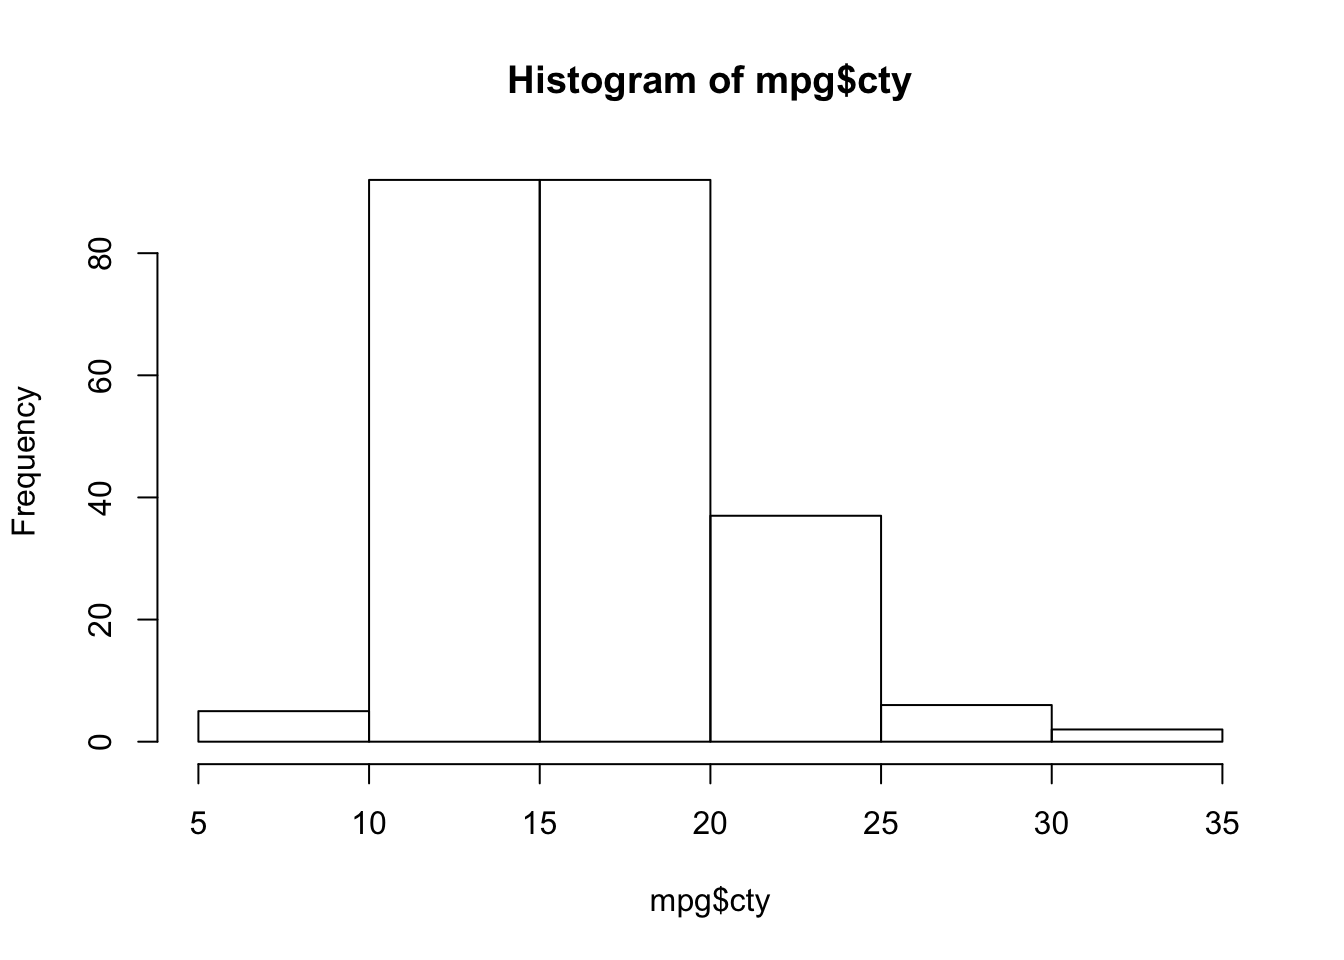
\includegraphics{ScPoEconometrics_files/figure-latex/unnamed-chunk-76-1} \end{center}

The histogram function has a number of parameters which can be changed
to make our plot look much nicer. Use the \texttt{?} operator to read
the documentation for the \texttt{hist()} to see a full list of these
parameters.

\begin{Shaded}
\begin{Highlighting}[]
\KeywordTok{hist}\NormalTok{(mpg}\OperatorTok{$}\NormalTok{cty,}
     \DataTypeTok{xlab   =} \StringTok{"Miles Per Gallon (City)"}\NormalTok{,}
     \DataTypeTok{main   =} \StringTok{"Histogram of MPG (City)"}\NormalTok{, }\CommentTok{# main title}
     \DataTypeTok{breaks =} \DecValTok{12}\NormalTok{,   }\CommentTok{# how many breaks?}
     \DataTypeTok{col    =} \StringTok{"red"}\NormalTok{,}
     \DataTypeTok{border =} \StringTok{"blue"}\NormalTok{)}
\end{Highlighting}
\end{Shaded}

\begin{center}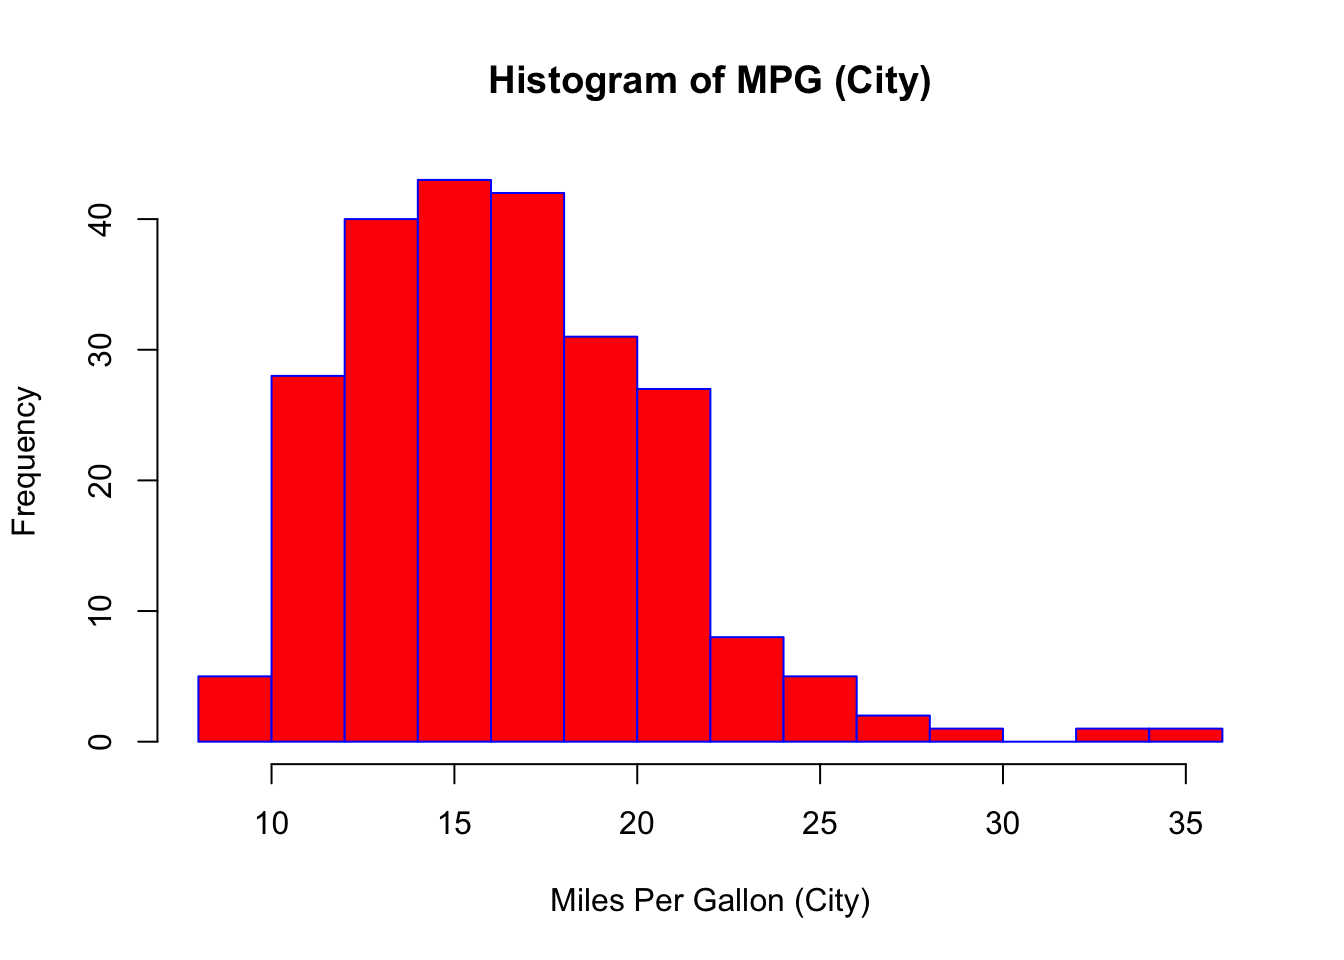
\includegraphics{ScPoEconometrics_files/figure-latex/unnamed-chunk-77-1} \end{center}

Importantly, you should always be sure to label your axes and give the
plot a title. The argument \texttt{breaks} is specific to
\texttt{hist()}. Entering an integer will give a suggestion to
\texttt{R} for how many bars to use for the histogram. By default
\texttt{R} will attempt to intelligently guess a good number of
\texttt{breaks}, but as we can see here, it is sometimes useful to
modify this yourself.

\subsection{Barplots}\label{barplots}

Somewhat similar to a histogram, a barplot can provide a visual summary
of a categorical variable, or a numeric variable with a finite number of
values, like a ranking from 1 to 10.

\begin{Shaded}
\begin{Highlighting}[]
\KeywordTok{barplot}\NormalTok{(}\KeywordTok{table}\NormalTok{(mpg}\OperatorTok{$}\NormalTok{drv))}
\end{Highlighting}
\end{Shaded}

\begin{center}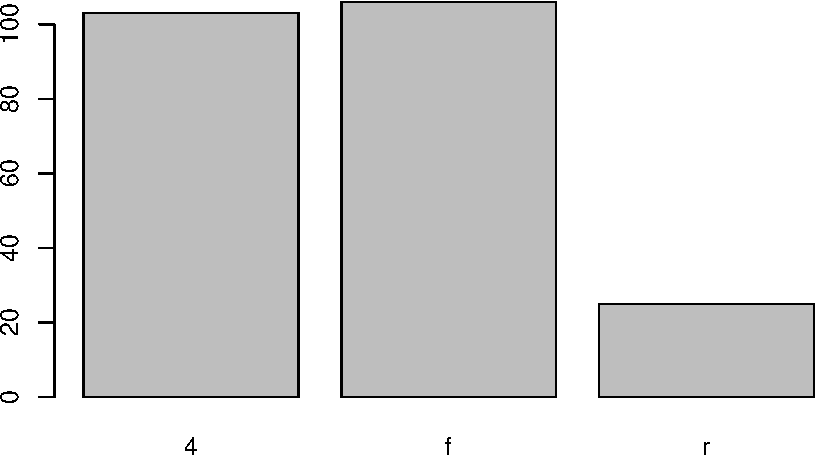
\includegraphics{ScPoEconometrics_files/figure-latex/unnamed-chunk-78-1} \end{center}

\begin{Shaded}
\begin{Highlighting}[]
\KeywordTok{barplot}\NormalTok{(}\KeywordTok{table}\NormalTok{(mpg}\OperatorTok{$}\NormalTok{drv),}
        \DataTypeTok{xlab   =} \StringTok{"Drivetrain (f = FWD, r = RWD, 4 = 4WD)"}\NormalTok{,}
        \DataTypeTok{ylab   =} \StringTok{"Frequency"}\NormalTok{,}
        \DataTypeTok{main   =} \StringTok{"Drivetrains"}\NormalTok{,}
        \DataTypeTok{col    =} \StringTok{"dodgerblue"}\NormalTok{,}
        \DataTypeTok{border =} \StringTok{"darkorange"}\NormalTok{)}
\end{Highlighting}
\end{Shaded}

\begin{center}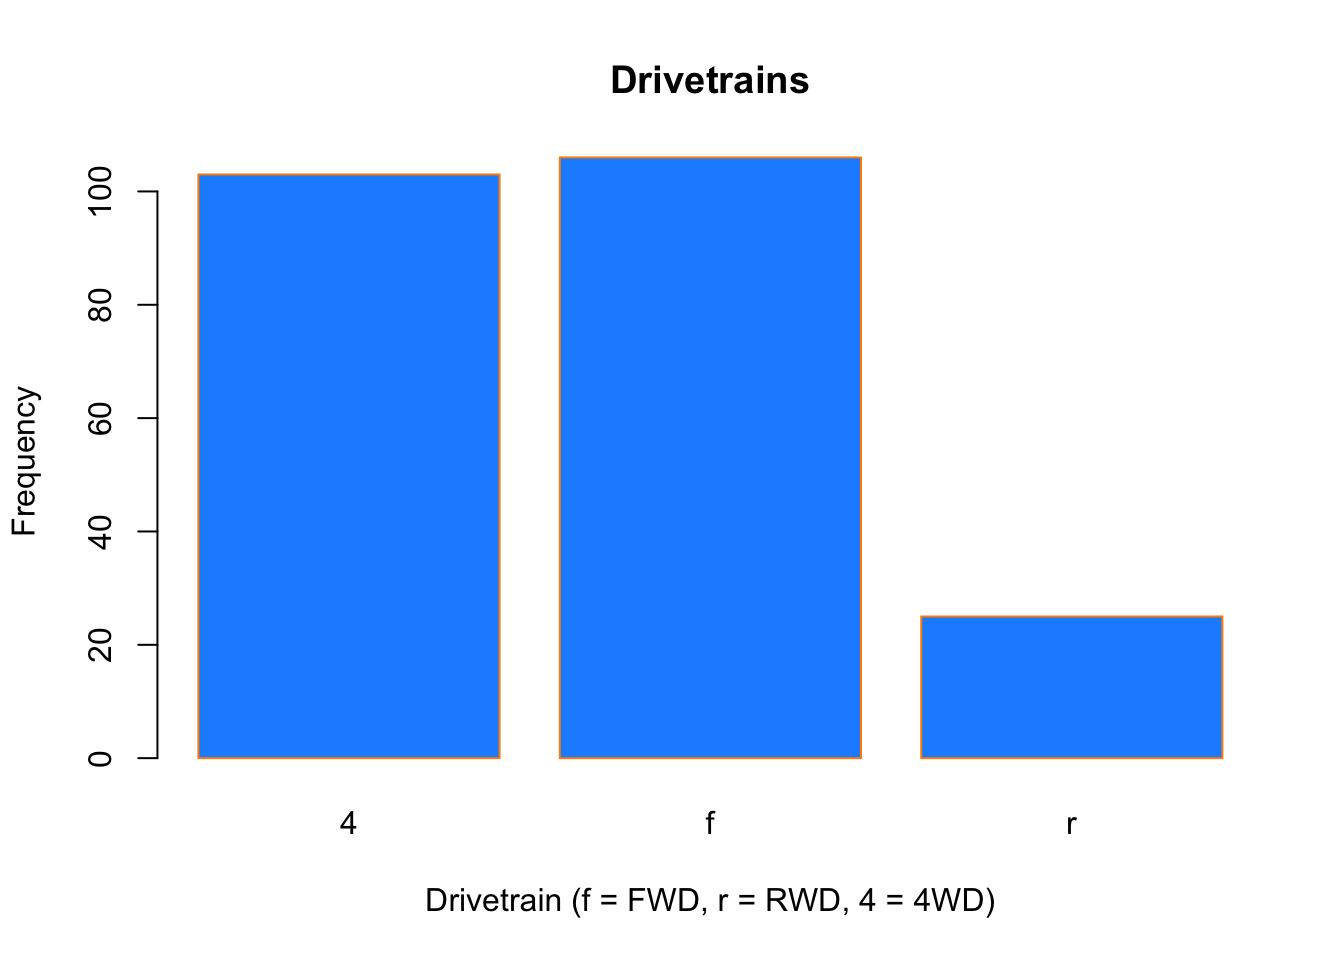
\includegraphics{ScPoEconometrics_files/figure-latex/unnamed-chunk-79-1} \end{center}

\subsection{Boxplots}\label{boxplots}

To visualize the relationship between a numerical and categorical
variable, once could use a \textbf{boxplot}. In the \texttt{mpg}
dataset, the \texttt{drv} variable takes a small, finite number of
values. A car can only be front wheel drive, 4 wheel drive, or rear
wheel drive.

\begin{Shaded}
\begin{Highlighting}[]
\KeywordTok{unique}\NormalTok{(mpg}\OperatorTok{$}\NormalTok{drv)}
\end{Highlighting}
\end{Shaded}

\begin{verbatim}
#OUT> [1] "f" "4" "r"
\end{verbatim}

First note that we can use a single boxplot as an alternative to a
histogram for visualizing a single numerical variable. To do so in
\texttt{R}, we use the \texttt{boxplot()} function. The box shows the
\emph{interquartile range}, the solid line in the middle is the value of
the median, the wiskers show 1.5 times the interquartile range, and the
dots are outliers.

\begin{Shaded}
\begin{Highlighting}[]
\KeywordTok{boxplot}\NormalTok{(mpg}\OperatorTok{$}\NormalTok{hwy)}
\end{Highlighting}
\end{Shaded}

\begin{center}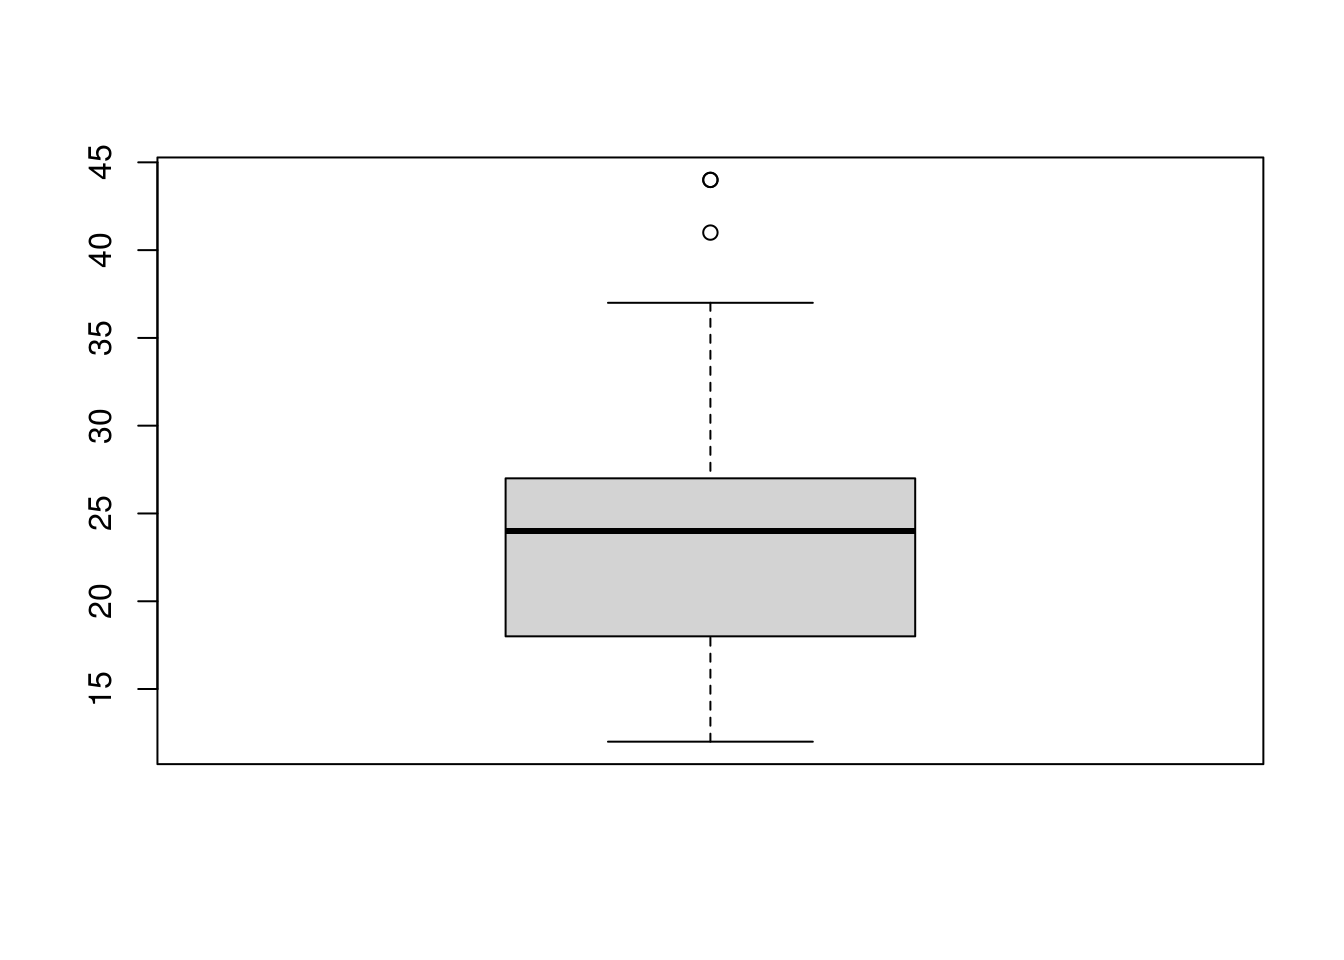
\includegraphics{ScPoEconometrics_files/figure-latex/unnamed-chunk-81-1} \end{center}

However, more often we will use boxplots to compare a numerical variable
for different values of a categorical variable.

\begin{Shaded}
\begin{Highlighting}[]
\KeywordTok{boxplot}\NormalTok{(hwy }\OperatorTok{~}\StringTok{ }\NormalTok{drv, }\DataTypeTok{data =}\NormalTok{ mpg)}
\end{Highlighting}
\end{Shaded}

\begin{center}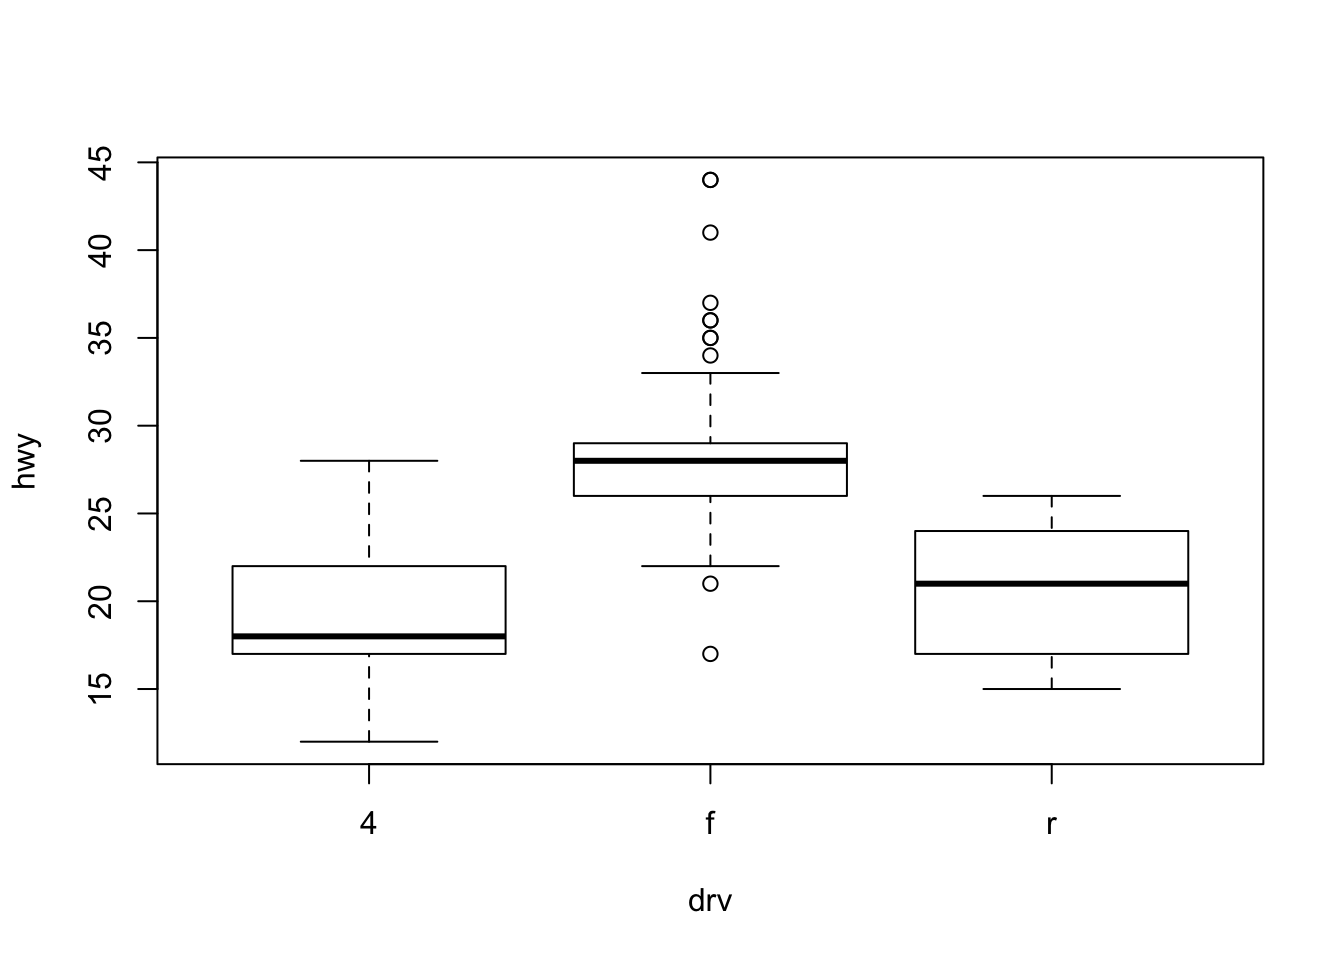
\includegraphics{ScPoEconometrics_files/figure-latex/unnamed-chunk-82-1} \end{center}

Here used the \texttt{boxplot()} command to create side-by-side
boxplots. However, since we are now dealing with two variables, the
syntax has changed. The \texttt{R} syntax
\texttt{hwy\ \textasciitilde{}\ drv,\ data\ =\ mpg} reads ``Plot the
\texttt{hwy} variable against the \texttt{drv} variable using the
dataset \texttt{mpg}.'' We see the use of a \texttt{\textasciitilde{}}
(which specifies a formula) and also a \texttt{data\ =} argument. This
will be a syntax that is common to many functions we will use in this
course.

\begin{Shaded}
\begin{Highlighting}[]
\KeywordTok{boxplot}\NormalTok{(hwy }\OperatorTok{~}\StringTok{ }\NormalTok{drv, }\DataTypeTok{data =}\NormalTok{ mpg,}
     \DataTypeTok{xlab   =} \StringTok{"Drivetrain (f = FWD, r = RWD, 4 = 4WD)"}\NormalTok{,}
     \DataTypeTok{ylab   =} \StringTok{"Miles Per Gallon (Highway)"}\NormalTok{,}
     \DataTypeTok{main   =} \StringTok{"MPG (Highway) vs Drivetrain"}\NormalTok{,}
     \DataTypeTok{pch    =} \DecValTok{20}\NormalTok{,}
     \DataTypeTok{cex    =} \DecValTok{2}\NormalTok{,}
     \DataTypeTok{col    =} \StringTok{"darkorange"}\NormalTok{,}
     \DataTypeTok{border =} \StringTok{"dodgerblue"}\NormalTok{)}
\end{Highlighting}
\end{Shaded}

\begin{center}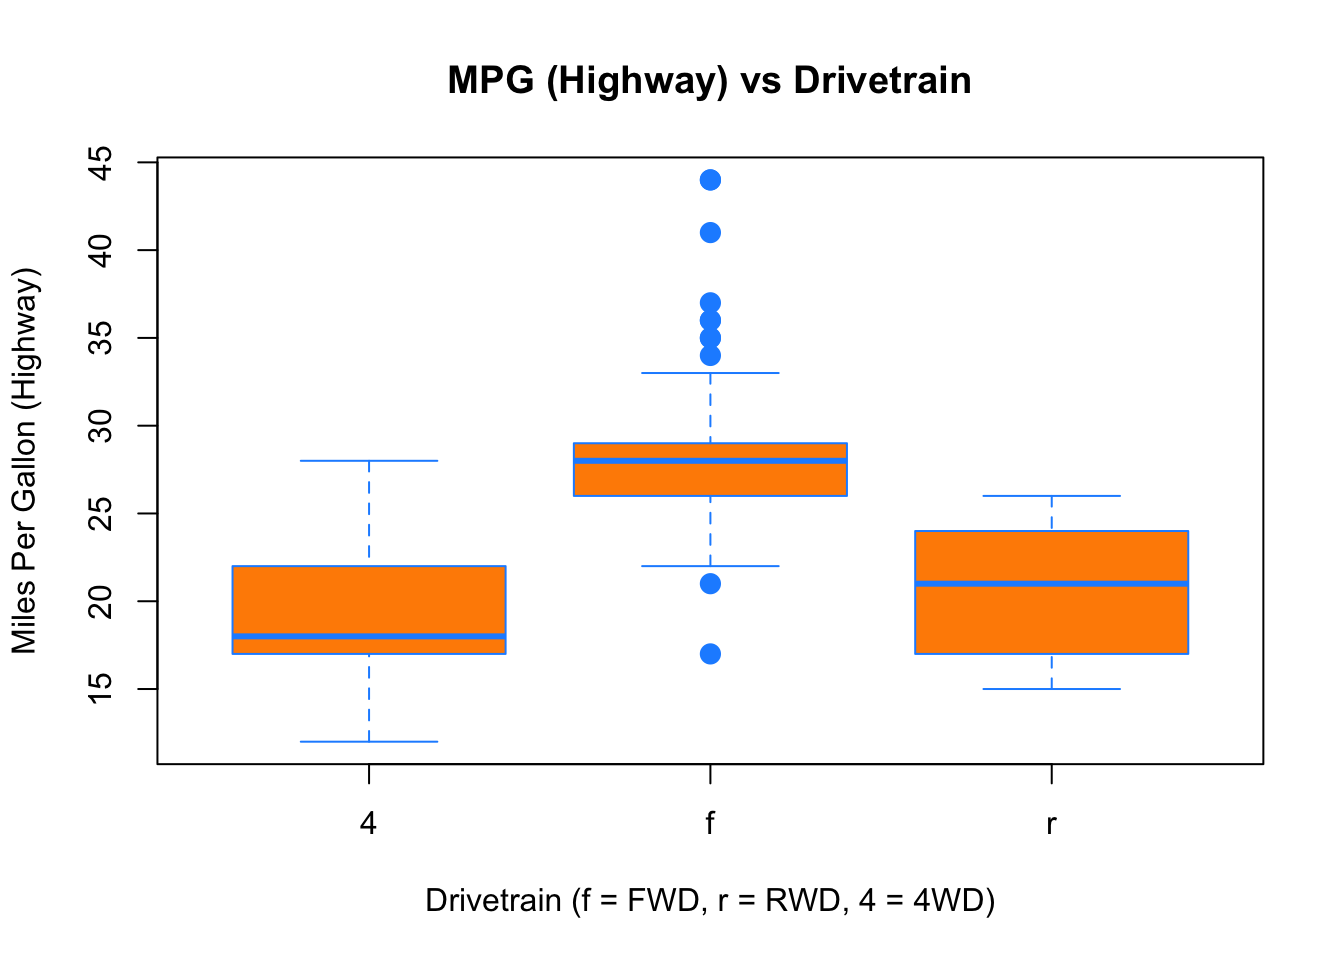
\includegraphics{ScPoEconometrics_files/figure-latex/unnamed-chunk-83-1} \end{center}

Again, \texttt{boxplot()} has a number of additional arguments which
have the ability to make our plot more visually appealing.

\subsection{Scatterplots}\label{scatterplots}

Lastly, to visualize the relationship between two numeric variables we
will use a \textbf{scatterplot}. This can be done with the
\texttt{plot()} function and the \texttt{\textasciitilde{}} syntax we
just used with a boxplot. (The function \texttt{plot()} can also be used
more generally; see the documentation for details.)

\begin{Shaded}
\begin{Highlighting}[]
\KeywordTok{plot}\NormalTok{(hwy }\OperatorTok{~}\StringTok{ }\NormalTok{displ, }\DataTypeTok{data =}\NormalTok{ mpg)}
\end{Highlighting}
\end{Shaded}

\begin{center}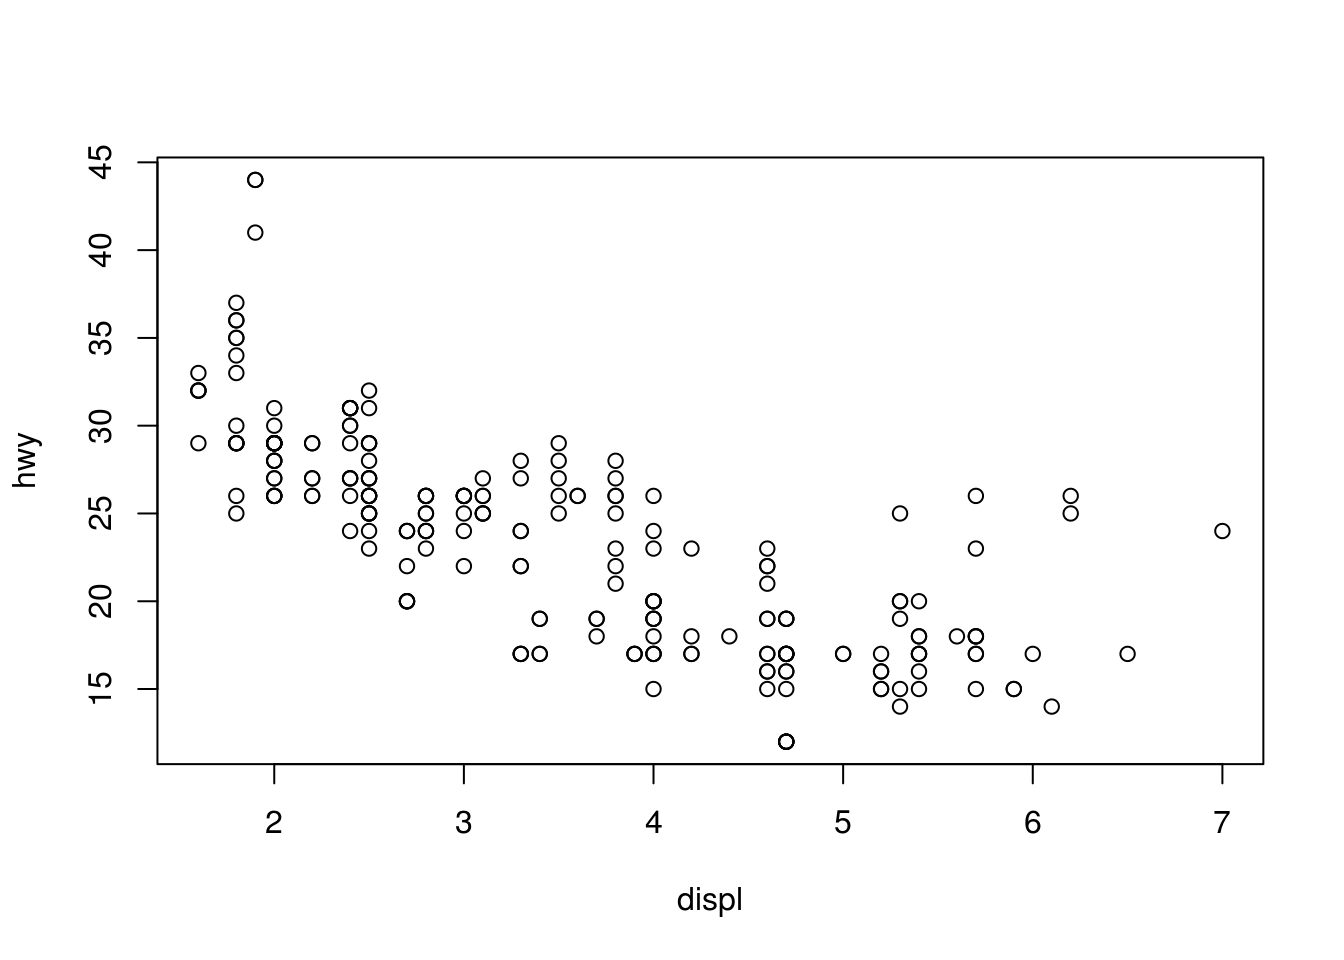
\includegraphics{ScPoEconometrics_files/figure-latex/unnamed-chunk-84-1} \end{center}

\begin{Shaded}
\begin{Highlighting}[]
\KeywordTok{plot}\NormalTok{(hwy }\OperatorTok{~}\StringTok{ }\NormalTok{displ, }\DataTypeTok{data =}\NormalTok{ mpg,}
     \DataTypeTok{xlab =} \StringTok{"Engine Displacement (in Liters)"}\NormalTok{,}
     \DataTypeTok{ylab =} \StringTok{"Miles Per Gallon (Highway)"}\NormalTok{,}
     \DataTypeTok{main =} \StringTok{"MPG (Highway) vs Engine Displacement"}\NormalTok{,}
     \DataTypeTok{pch  =} \DecValTok{20}\NormalTok{,}
     \DataTypeTok{cex  =} \DecValTok{2}\NormalTok{,}
     \DataTypeTok{col  =} \StringTok{"dodgerblue"}\NormalTok{)}
\end{Highlighting}
\end{Shaded}

\begin{center}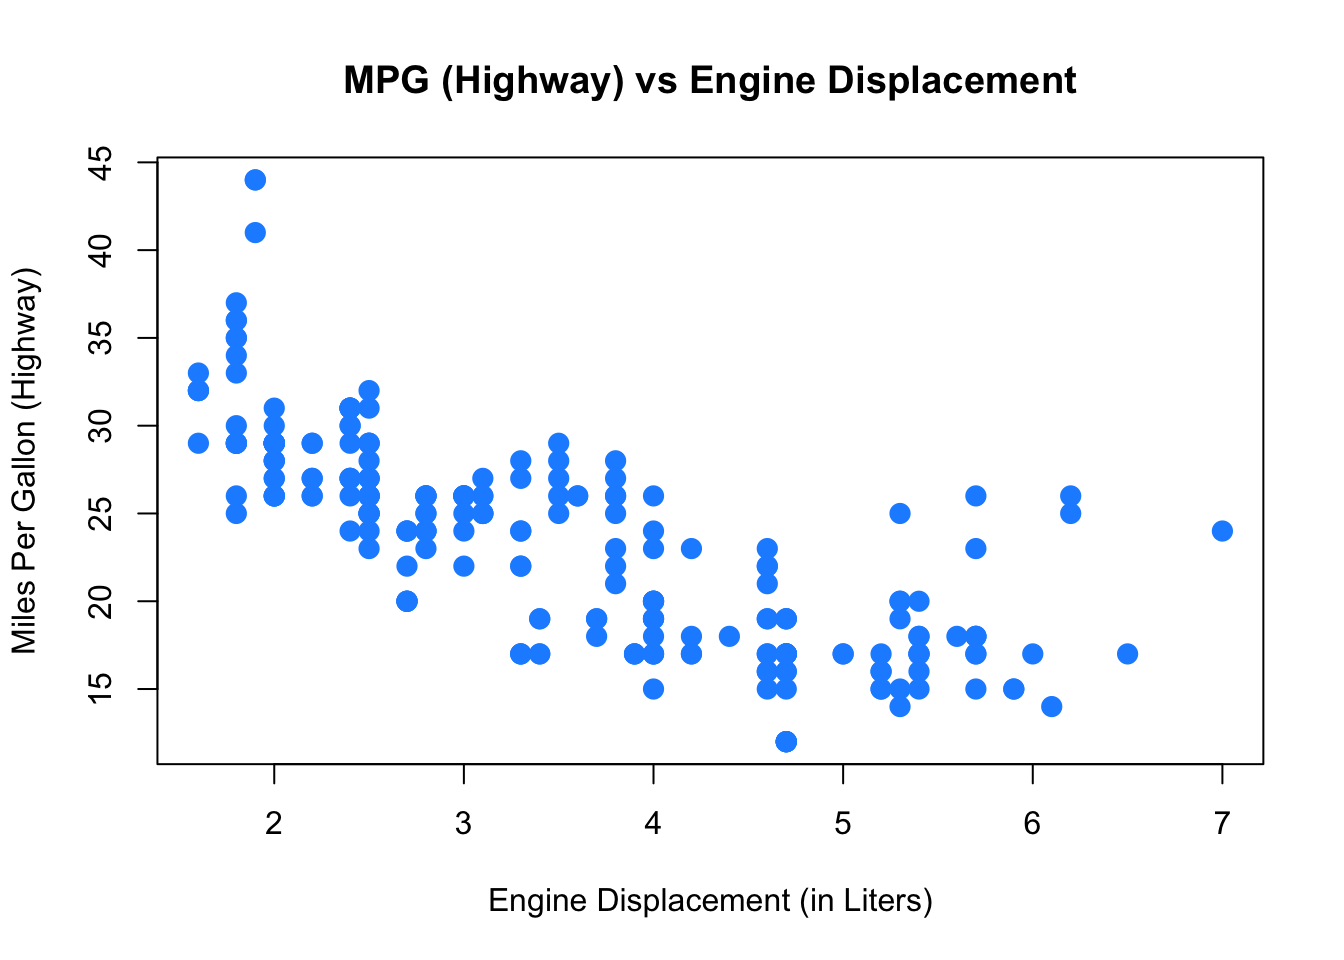
\includegraphics{ScPoEconometrics_files/figure-latex/unnamed-chunk-85-1} \end{center}

\subsection{\texorpdfstring{\texttt{ggplot}}{ggplot}}\label{ggplot}

All of the above plots could also have been generated using the
\texttt{ggplot} function from the already loaded \texttt{ggplot2}
package. Which function you use is up to you, but sometimes a plot is
easier to build in base R (like in the \texttt{boxplot} example maybe),
sometimes the other way around.

\begin{Shaded}
\begin{Highlighting}[]
\KeywordTok{ggplot}\NormalTok{(}\DataTypeTok{data =}\NormalTok{ mpg,}\DataTypeTok{mapping =} \KeywordTok{aes}\NormalTok{(}\DataTypeTok{x=}\NormalTok{displ,}\DataTypeTok{y=}\NormalTok{hwy)) }\OperatorTok{+}\StringTok{ }\KeywordTok{geom_point}\NormalTok{()}
\end{Highlighting}
\end{Shaded}

\begin{center}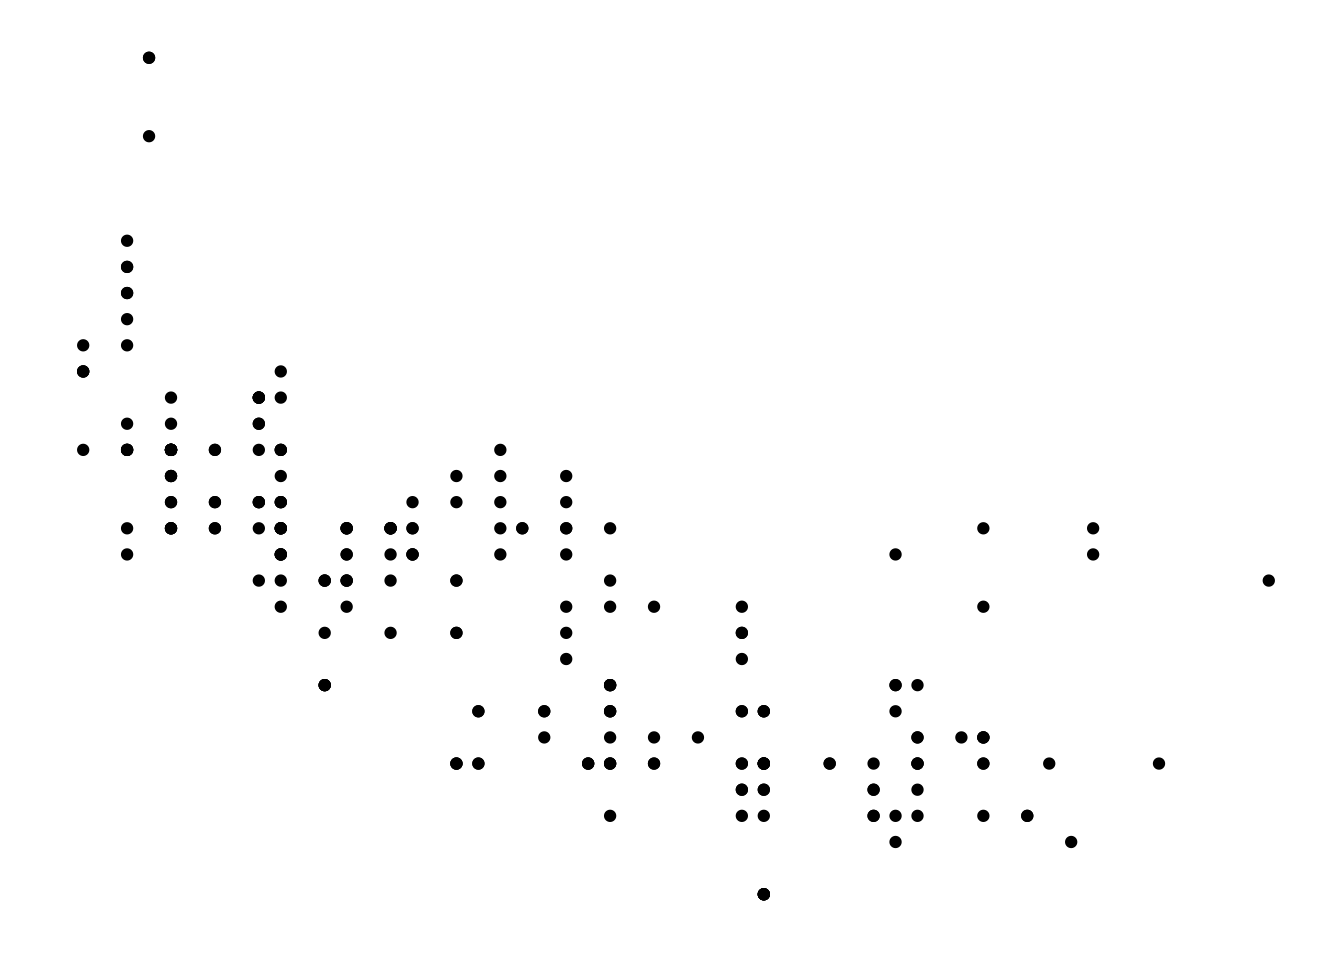
\includegraphics{ScPoEconometrics_files/figure-latex/unnamed-chunk-86-1} \end{center}

\texttt{ggplot} is impossible to describe in brief terms, so please look
at \href{http://ggplot2.tidyverse.org}{the package's website} which
provides excellent guidance. We will from time to time use ggplot in
this book, so you could familiarize yourself with it. Let's quickly
demonstrate how one could further customize that first plot:

\begin{Shaded}
\begin{Highlighting}[]
\KeywordTok{ggplot}\NormalTok{(}\DataTypeTok{data =}\NormalTok{ mpg, }\DataTypeTok{mapping =} \KeywordTok{aes}\NormalTok{(}\DataTypeTok{x=}\NormalTok{displ,}\DataTypeTok{y=}\NormalTok{hwy)) }\OperatorTok{+}\StringTok{   }\CommentTok{# ggplot() makes base plot}
\StringTok{  }\KeywordTok{geom_point}\NormalTok{(}\DataTypeTok{color=}\StringTok{"blue"}\NormalTok{,}\DataTypeTok{size=}\DecValTok{2}\NormalTok{) }\OperatorTok{+}\StringTok{     }\CommentTok{# how to show x and y?}
\StringTok{  }\KeywordTok{scale_y_continuous}\NormalTok{(}\DataTypeTok{name=}\StringTok{"Miles Per Gallon (Highway)"}\NormalTok{) }\OperatorTok{+}\StringTok{  }\CommentTok{# name of y axis}
\StringTok{  }\KeywordTok{scale_x_continuous}\NormalTok{(}\DataTypeTok{name=}\StringTok{"Engine Displacement (in Liters)"}\NormalTok{) }\OperatorTok{+}\StringTok{ }\CommentTok{# x axis}
\StringTok{  }\KeywordTok{theme_bw}\NormalTok{() }\OperatorTok{+}\StringTok{    }\CommentTok{# change the background}
\StringTok{  }\KeywordTok{ggtitle}\NormalTok{(}\StringTok{"MPG (Highway) vs Engine Displacement"}\NormalTok{)   }\CommentTok{# add a title}
\end{Highlighting}
\end{Shaded}

\begin{center}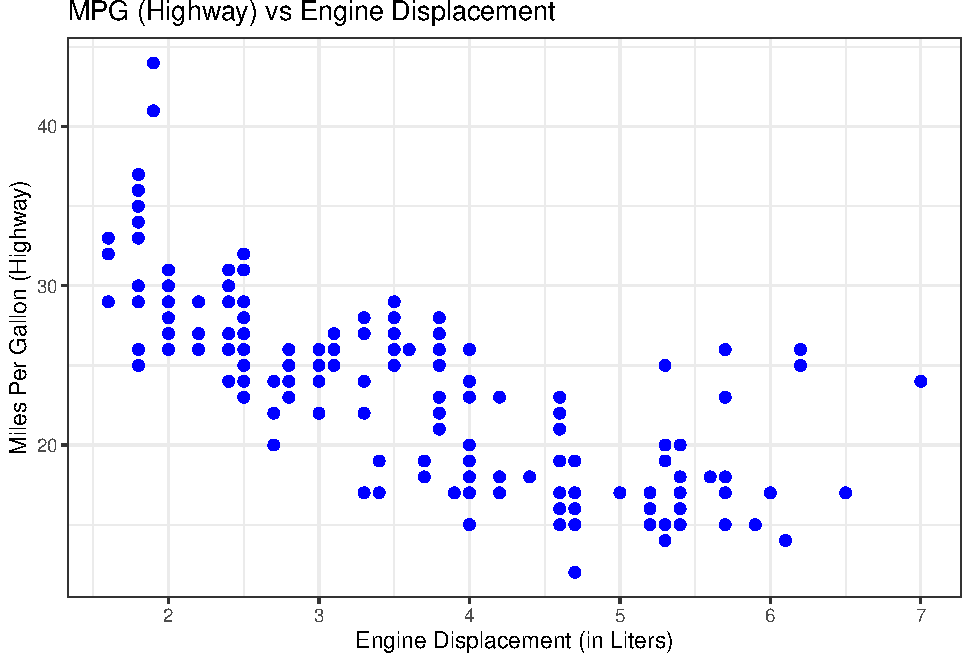
\includegraphics{ScPoEconometrics_files/figure-latex/unnamed-chunk-87-1} \end{center}

If you want to see \texttt{ggplot} in action, you could start with
\href{http://jcyhong.github.io/ggplot_demo.html}{this} and then look at
that
\href{https://tutorials.iq.harvard.edu/R/Rgraphics/Rgraphics.html}{very
nice tutorial}? It's fun!

\section{Summarizing Two Variables}\label{summarize-two}

We often are interested in how two variables are related to each other.
The core concepts here are \emph{covariance} and \emph{correlation}.
Let's generate some data on \texttt{x} and \texttt{y} and plot them
against each other:

\begin{figure}

{\centering 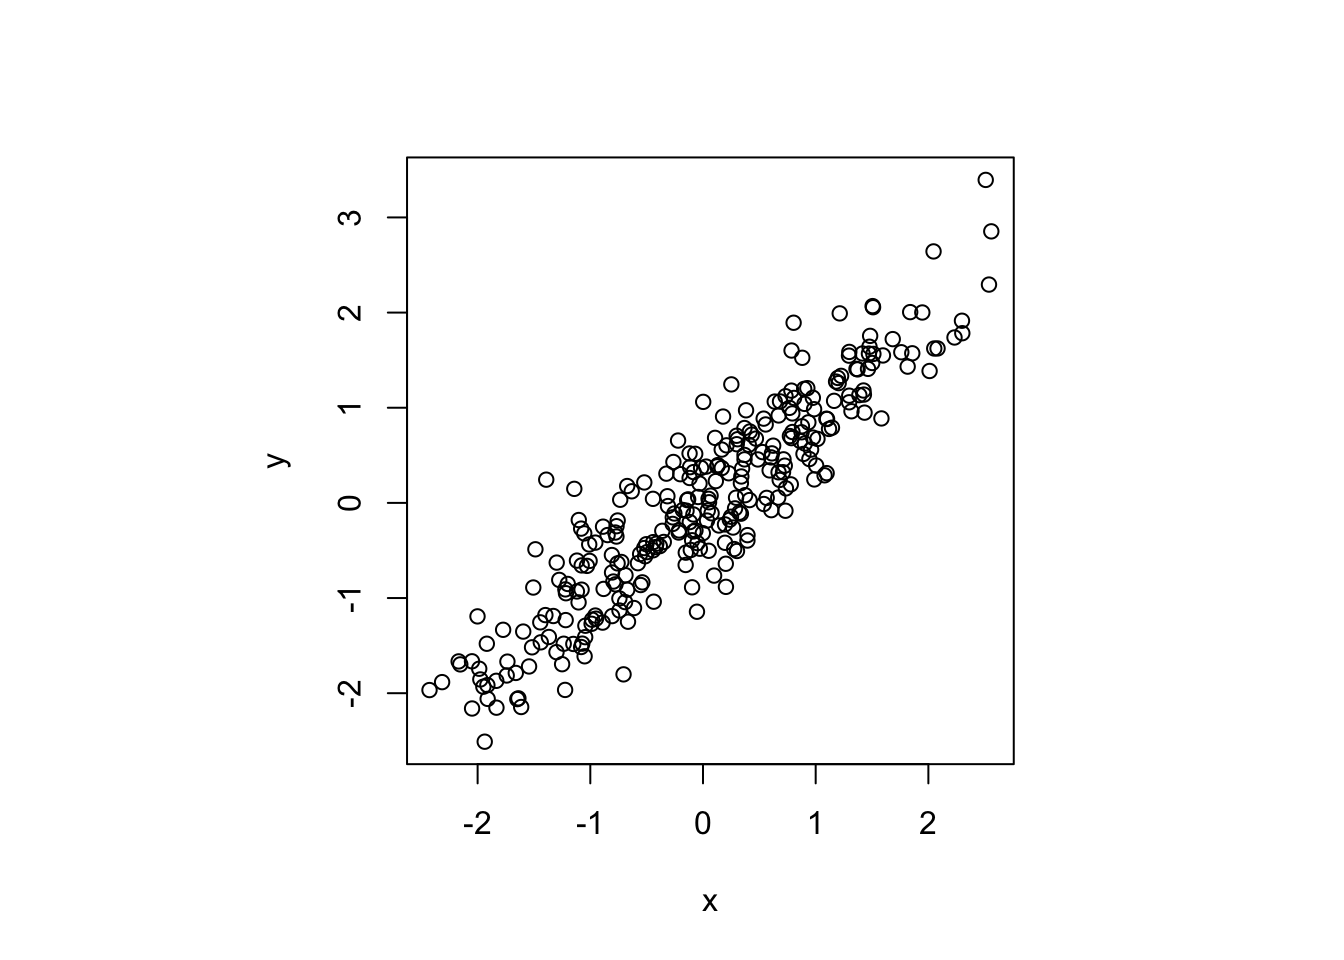
\includegraphics{ScPoEconometrics_files/figure-latex/x-y-corr-1} 

}

\caption{How are $x$ and $y$ related?}\label{fig:x-y-corr}
\end{figure}

Taking as example the data in this plot, the concepts \emph{covariance}
and \emph{correlation} relate to the following type of question:

\begin{note}
Given we observe value of something like \(x=2\), say, can we expect a
high or a low value of \(y\), on average? Something like \(y=2\) or
rather something like \(y=-2\)?
\end{note}

 The answer to this type of question can be addressed by computing the
covariance of both variables:

\begin{Shaded}
\begin{Highlighting}[]
\KeywordTok{cov}\NormalTok{(x,y)  }
\end{Highlighting}
\end{Shaded}

\begin{verbatim}
#OUT> [1] 1.041195
\end{verbatim}

Here, this gives a positive number, 1.04, indicating that as one
variable lies above it's average, the other one does as well. In other
words, it indicates a \textbf{positive relationship}. What is less
clear, however, how to interpret the magnitude of 1.04. Is that a
\emph{strong} or a \emph{weak} positive association?

In fact, we cannot tell. This is because the covariance is measured in
the same units as the data, and those units often differ between both
variables. There is a better measure available to us though, the
\textbf{correlation}, which is obtained by \emph{standardizing} each
variable. By \emph{standardizing} a variable \(x\) one means to divide
\(x\) by its standard deviation \(\sigma_x\):

\[
z = \frac{x}{\sigma_x}
\]

The \emph{correlation coefficient} between \(x\) and \(y\), commonly
denoted \(r_{x,y}\), is then defined as

\[
r_{x,y} = \frac{cov(x,y)}{\sigma_x \sigma_y},
\]

and we get rid of the units problem. In \texttt{R}, you can call
directly

\begin{Shaded}
\begin{Highlighting}[]
\KeywordTok{cor}\NormalTok{(x,y)}
\end{Highlighting}
\end{Shaded}

\begin{verbatim}
#OUT> [1] 0.9142495
\end{verbatim}

Now this is better. Given that the correlation has to lie in \([-1,1]\),
a value of 0.91 is indicative of a rather strong positive relationship
for the data in figure \ref{fig:x-y-corr}

Note that \(x,y\) being drawn from a \emph{continuous distribution}
(they are joint normally distributed) had no implication for covariance
and correlation: We can compute those measures also for discrete random
variables (like the throws of two dice, as you will see in one of our
tutorials).

\subsection{\texorpdfstring{Visually estimating
\(\sigma\)}{Visually estimating \textbackslash{}sigma}}\label{visually-estimating-sigma}

Sometimes it is useful to estimate the standard deviation of some data
\emph{without} the help of a computer (for example during an exam ;-) ).
If \(x\) is approximately normally distributed, 95\% of its observations
will lie within a range of \(\bar{x}\pm\) two standard deviations of
\(x\). That is to say, \emph{four} standard deviations of \(x\) cover
95\% of its observations. Hence, a simple way to estimate the standard
deviation for a variable is to look at the range of \(x\), and simply
divide that number by four.

\begin{figure}

{\centering 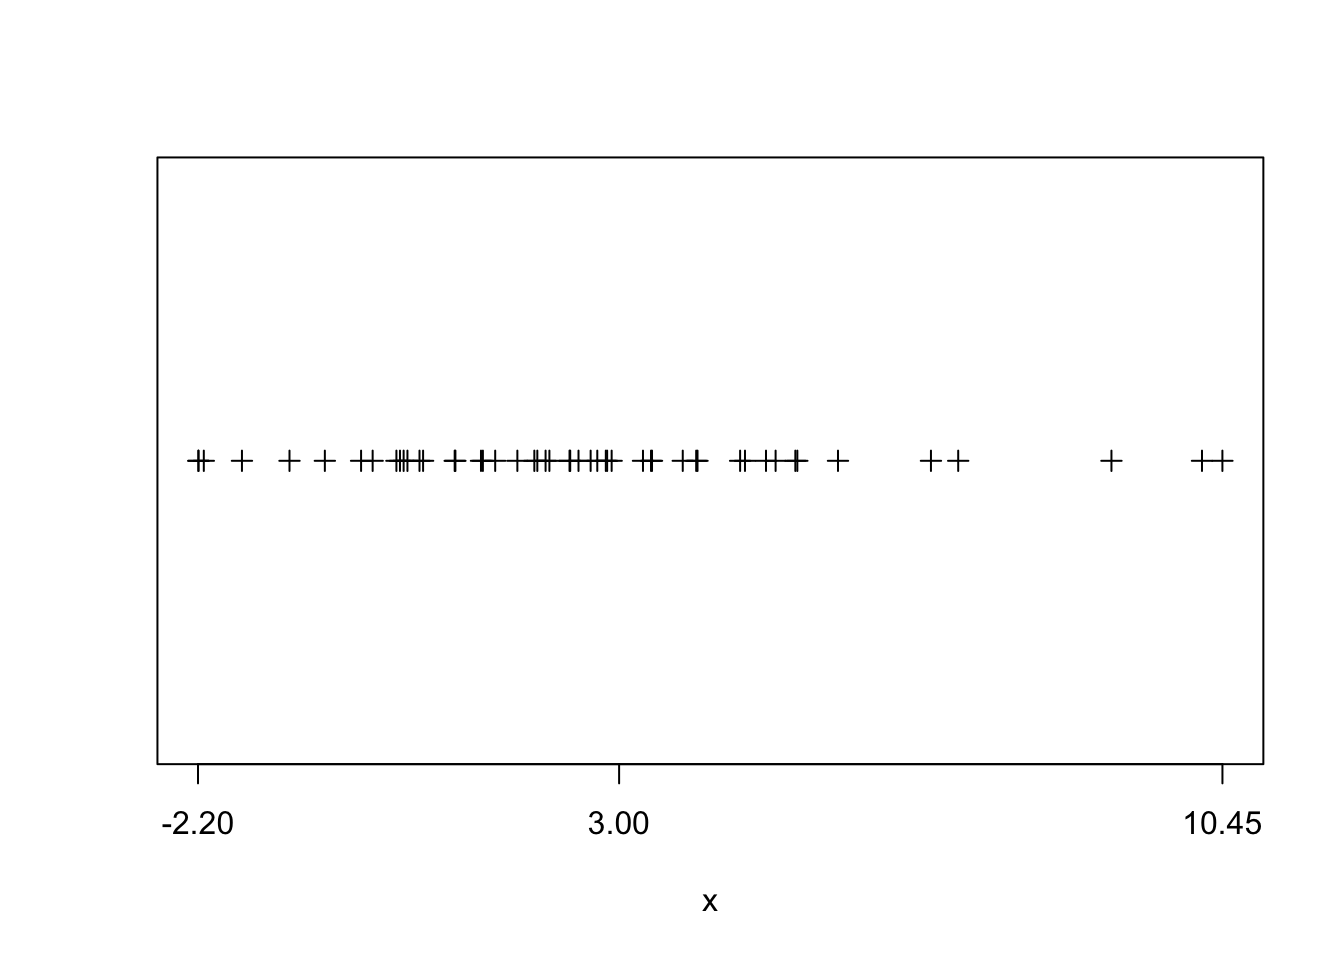
\includegraphics{ScPoEconometrics_files/figure-latex/vis-1} 

}

\caption{visual estimation on $\sigma$. The x-axis labels min and max as well as mean of $x$.}\label{fig:vis}
\end{figure}

This is illustrated in figure \ref{fig:vis}. Here we see that
\texttt{range(x)/4} gives 3.16 which compares favourably to the actual
standard deviation 3.

\section{\texorpdfstring{The
\texttt{tidyverse}}{The tidyverse}}\label{the-tidyverse}

\href{http://hadley.nz}{Hadley Wickham} is the author of R packages
\texttt{ggplot2} and also of \texttt{dplyr} (and also a myriad of
others). With \texttt{ggplot2} he introduced what is called the
\emph{grammar of graphics} (hence, \texttt{gg}) to \texttt{R}. Grammar
in the sense that there are \textbf{nouns} and \textbf{verbs} and a
\textbf{syntax}, i.e.~rules of how nouns and verbs are to be put
together to construct an understandable sentence. He has extended the
\emph{grammar} idea into various other packages. The \texttt{tidyverse}
package is a collection of those packages.

\texttt{tidy} data is data where:

\begin{itemize}
\tightlist
\item
  Each variable is a column
\item
  Each observation is a row
\item
  Each value is a cell
\end{itemize}

Fair enough, you might say, that is a regular spreadsheet. And you are
right! However, data comes to us \emph{not} tidy most of the times, and
we first need to clean, or \texttt{tidy}, it up. Once it's in
\texttt{tidy} format, we can use the tools in the \texttt{tidyverse}
with great efficiency to analyse the data and stop worrying about which
tool to use.

\subsection{\texorpdfstring{Reading \texttt{.csv} data in the
\emph{tidy}
way}{Reading .csv data in the tidy way}}\label{reading-.csv-data-in-the-tidy-way}

We could have used the \texttt{read\_csv()} function from the
\texttt{readr} package to read our example dataset from the previous
chapter. The \texttt{readr} function \texttt{read\_csv()} has a number
of advantages over the built-in \texttt{read.csv}. For example, it is
much faster reading larger data.
\href{https://cran.r-project.org/web/packages/tibble/vignettes/tibble.html}{It
also uses the \texttt{tibble} package to read the data as a tibble.}
\textbf{A \texttt{tibble} is simply a data frame that prints with
sanity.} Notice in the output below that we are given additional
information such as dimension and variable type.

\begin{Shaded}
\begin{Highlighting}[]
\KeywordTok{library}\NormalTok{(readr)  }\CommentTok{# you need `install.packages("readr")` once!}
\NormalTok{path =}\StringTok{ }\KeywordTok{system.file}\NormalTok{(}\DataTypeTok{package=}\StringTok{"ScPoEconometrics"}\NormalTok{,}\StringTok{"datasets"}\NormalTok{,}\StringTok{"example-data.csv"}\NormalTok{)}
\NormalTok{example_data_from_disk =}\StringTok{ }\KeywordTok{read_csv}\NormalTok{(path)}
\end{Highlighting}
\end{Shaded}

\subsection{\texorpdfstring{Tidy \texttt{data.frames} are
\texttt{tibbles}}{Tidy data.frames are tibbles}}\label{tidy-data.frames-are-tibbles}

Let's grab some data from the \texttt{ggplot2} package:

\begin{Shaded}
\begin{Highlighting}[]
\KeywordTok{data}\NormalTok{(mpg,}\DataTypeTok{package =} \StringTok{"ggplot2"}\NormalTok{)  }\CommentTok{# load dataset `mpg` from `ggplot2` package}
\KeywordTok{head}\NormalTok{(mpg, }\DataTypeTok{n =} \DecValTok{10}\NormalTok{)}
\end{Highlighting}
\end{Shaded}

\begin{verbatim}
#OUT> # A tibble: 10 x 11
#OUT>    manufacturer model    displ  year   cyl trans   drv     cty   hwy fl    class
#OUT>    <chr>        <chr>    <dbl> <int> <int> <chr>   <chr> <int> <int> <chr> <chr>
#OUT>  1 audi         a4         1.8  1999     4 auto(l~ f        18    29 p     comp~
#OUT>  2 audi         a4         1.8  1999     4 manual~ f        21    29 p     comp~
#OUT>  3 audi         a4         2    2008     4 manual~ f        20    31 p     comp~
#OUT>  4 audi         a4         2    2008     4 auto(a~ f        21    30 p     comp~
#OUT>  5 audi         a4         2.8  1999     6 auto(l~ f        16    26 p     comp~
#OUT>  6 audi         a4         2.8  1999     6 manual~ f        18    26 p     comp~
#OUT>  7 audi         a4         3.1  2008     6 auto(a~ f        18    27 p     comp~
#OUT>  8 audi         a4 quat~   1.8  1999     4 manual~ 4        18    26 p     comp~
#OUT>  9 audi         a4 quat~   1.8  1999     4 auto(l~ 4        16    25 p     comp~
#OUT> 10 audi         a4 quat~   2    2008     4 manual~ 4        20    28 p     comp~
\end{verbatim}

The function \texttt{head()} will display the first \texttt{n}
observations of the data frame, as we have seen. The \texttt{head()}
function was more useful before tibbles. Notice that \texttt{mpg} is a
tibble already, so the output from \texttt{head()} indicates there are
only \texttt{10} observations. Note that this applies to
\texttt{head(mpg,\ n\ =\ 10)} and not \texttt{mpg} itself. Also note
that tibbles print a limited number of rows and columns by default. The
last line of the printed output indicates with rows and columns were
omitted.

\begin{Shaded}
\begin{Highlighting}[]
\NormalTok{mpg}
\end{Highlighting}
\end{Shaded}

\begin{verbatim}
#OUT> # A tibble: 234 x 11
#OUT>    manufacturer model    displ  year   cyl trans   drv     cty   hwy fl    class
#OUT>    <chr>        <chr>    <dbl> <int> <int> <chr>   <chr> <int> <int> <chr> <chr>
#OUT>  1 audi         a4         1.8  1999     4 auto(l~ f        18    29 p     comp~
#OUT>  2 audi         a4         1.8  1999     4 manual~ f        21    29 p     comp~
#OUT>  3 audi         a4         2    2008     4 manual~ f        20    31 p     comp~
#OUT>  4 audi         a4         2    2008     4 auto(a~ f        21    30 p     comp~
#OUT>  5 audi         a4         2.8  1999     6 auto(l~ f        16    26 p     comp~
#OUT>  6 audi         a4         2.8  1999     6 manual~ f        18    26 p     comp~
#OUT>  7 audi         a4         3.1  2008     6 auto(a~ f        18    27 p     comp~
#OUT>  8 audi         a4 quat~   1.8  1999     4 manual~ 4        18    26 p     comp~
#OUT>  9 audi         a4 quat~   1.8  1999     4 auto(l~ 4        16    25 p     comp~
#OUT> 10 audi         a4 quat~   2    2008     4 manual~ 4        20    28 p     comp~
#OUT> # ... with 224 more rows
\end{verbatim}

Let's look at \texttt{str} as well to get familiar with the content of
the data:

\begin{Shaded}
\begin{Highlighting}[]
\KeywordTok{str}\NormalTok{(mpg)}
\end{Highlighting}
\end{Shaded}

\begin{verbatim}
#OUT> Classes 'tbl_df', 'tbl' and 'data.frame': 234 obs. of  11 variables:
#OUT>  $ manufacturer: chr  "audi" "audi" "audi" "audi" ...
#OUT>  $ model       : chr  "a4" "a4" "a4" "a4" ...
#OUT>  $ displ       : num  1.8 1.8 2 2 2.8 2.8 3.1 1.8 1.8 2 ...
#OUT>  $ year        : int  1999 1999 2008 2008 1999 1999 2008 1999 1999 2008 ...
#OUT>  $ cyl         : int  4 4 4 4 6 6 6 4 4 4 ...
#OUT>  $ trans       : chr  "auto(l5)" "manual(m5)" "manual(m6)" "auto(av)" ...
#OUT>  $ drv         : chr  "f" "f" "f" "f" ...
#OUT>  $ cty         : int  18 21 20 21 16 18 18 18 16 20 ...
#OUT>  $ hwy         : int  29 29 31 30 26 26 27 26 25 28 ...
#OUT>  $ fl          : chr  "p" "p" "p" "p" ...
#OUT>  $ class       : chr  "compact" "compact" "compact" "compact" ...
\end{verbatim}

In this dataset an observation is for a particular model-year of a car,
and the variables describe attributes of the car, for example its
highway fuel efficiency.

To understand more about the data set, we use the \texttt{?} operator to
pull up the documentation for the data.

\begin{Shaded}
\begin{Highlighting}[]
\NormalTok{?mpg}
\end{Highlighting}
\end{Shaded}

Working with tibbles is mostly the same as working with plain
data.frames:

\begin{Shaded}
\begin{Highlighting}[]
\KeywordTok{names}\NormalTok{(mpg)}
\end{Highlighting}
\end{Shaded}

\begin{verbatim}
#OUT>  [1] "manufacturer" "model"        "displ"        "year"         "cyl"         
#OUT>  [6] "trans"        "drv"          "cty"          "hwy"          "fl"          
#OUT> [11] "class"
\end{verbatim}

\begin{Shaded}
\begin{Highlighting}[]
\NormalTok{mpg}\OperatorTok{$}\NormalTok{year}
\end{Highlighting}
\end{Shaded}

\begin{verbatim}
#OUT>   [1] 1999 1999 2008 2008 1999 1999 2008 1999 1999 2008 2008 1999 1999 2008 2008
#OUT>  [16] 1999 2008 2008 2008 2008 2008 1999 2008 1999 1999 2008 2008 2008 2008 2008
#OUT>  [31] 1999 1999 1999 2008 1999 2008 2008 1999 1999 1999 1999 2008 2008 2008 1999
#OUT>  [46] 1999 2008 2008 2008 2008 1999 1999 2008 2008 2008 1999 1999 1999 2008 2008
#OUT>  [61] 2008 1999 2008 1999 2008 2008 2008 2008 2008 2008 1999 1999 2008 1999 1999
#OUT>  [76] 1999 2008 1999 1999 1999 2008 2008 1999 1999 1999 1999 1999 2008 1999 2008
#OUT>  [91] 1999 1999 2008 2008 1999 1999 2008 2008 2008 1999 1999 1999 1999 1999 2008
#OUT> [106] 2008 2008 2008 1999 1999 2008 2008 1999 1999 2008 1999 1999 2008 2008 2008
#OUT> [121] 2008 2008 2008 2008 1999 1999 2008 2008 2008 2008 1999 2008 2008 1999 1999
#OUT> [136] 1999 2008 1999 2008 2008 1999 1999 1999 2008 2008 2008 2008 1999 1999 2008
#OUT> [151] 1999 1999 2008 2008 1999 1999 1999 2008 2008 1999 1999 2008 2008 2008 2008
#OUT> [166] 1999 1999 1999 1999 2008 2008 2008 2008 1999 1999 1999 1999 2008 2008 1999
#OUT> [181] 1999 2008 2008 1999 1999 2008 1999 1999 2008 2008 1999 1999 2008 1999 1999
#OUT> [196] 1999 2008 2008 1999 2008 1999 1999 2008 1999 1999 2008 2008 1999 1999 2008
#OUT> [211] 2008 1999 1999 1999 1999 2008 2008 2008 2008 1999 1999 1999 1999 1999 1999
#OUT> [226] 2008 2008 1999 1999 2008 2008 1999 1999 2008
\end{verbatim}

\begin{Shaded}
\begin{Highlighting}[]
\NormalTok{mpg}\OperatorTok{$}\NormalTok{hwy}
\end{Highlighting}
\end{Shaded}

\begin{verbatim}
#OUT>   [1] 29 29 31 30 26 26 27 26 25 28 27 25 25 25 25 24 25 23 20 15 20 17 17 26 23
#OUT>  [26] 26 25 24 19 14 15 17 27 30 26 29 26 24 24 22 22 24 24 17 22 21 23 23 19 18
#OUT>  [51] 17 17 19 19 12 17 15 17 17 12 17 16 18 15 16 12 17 17 16 12 15 16 17 15 17
#OUT>  [76] 17 18 17 19 17 19 19 17 17 17 16 16 17 15 17 26 25 26 24 21 22 23 22 20 33
#OUT> [101] 32 32 29 32 34 36 36 29 26 27 30 31 26 26 28 26 29 28 27 24 24 24 22 19 20
#OUT> [126] 17 12 19 18 14 15 18 18 15 17 16 18 17 19 19 17 29 27 31 32 27 26 26 25 25
#OUT> [151] 17 17 20 18 26 26 27 28 25 25 24 27 25 26 23 26 26 26 26 25 27 25 27 20 20
#OUT> [176] 19 17 20 17 29 27 31 31 26 26 28 27 29 31 31 26 26 27 30 33 35 37 35 15 18
#OUT> [201] 20 20 22 17 19 18 20 29 26 29 29 24 44 29 26 29 29 29 29 23 24 44 41 29 26
#OUT> [226] 28 29 29 29 28 29 26 26 26
\end{verbatim}

Subsetting is also similar to dataframe. Here, we find fuel efficient
vehicles earning over 35 miles per gallon and only display
\texttt{manufacturer}, \texttt{model} and \texttt{year}.

\begin{Shaded}
\begin{Highlighting}[]
\CommentTok{# mpg[row condition, col condition]}
\NormalTok{mpg[mpg}\OperatorTok{$}\NormalTok{hwy }\OperatorTok{>}\StringTok{ }\DecValTok{35}\NormalTok{, }\KeywordTok{c}\NormalTok{(}\StringTok{"manufacturer"}\NormalTok{, }\StringTok{"model"}\NormalTok{, }\StringTok{"year"}\NormalTok{)]}
\end{Highlighting}
\end{Shaded}

\begin{verbatim}
#OUT> # A tibble: 6 x 3
#OUT>   manufacturer model       year
#OUT>   <chr>        <chr>      <int>
#OUT> 1 honda        civic       2008
#OUT> 2 honda        civic       2008
#OUT> 3 toyota       corolla     2008
#OUT> 4 volkswagen   jetta       1999
#OUT> 5 volkswagen   new beetle  1999
#OUT> 6 volkswagen   new beetle  1999
\end{verbatim}

An alternative would be to use the \texttt{subset()} function, which has
a much more readable syntax.

\begin{Shaded}
\begin{Highlighting}[]
\KeywordTok{subset}\NormalTok{(mpg, }\DataTypeTok{subset =}\NormalTok{ hwy }\OperatorTok{>}\StringTok{ }\DecValTok{35}\NormalTok{, }\DataTypeTok{select =} \KeywordTok{c}\NormalTok{(}\StringTok{"manufacturer"}\NormalTok{, }\StringTok{"model"}\NormalTok{, }\StringTok{"year"}\NormalTok{))}
\end{Highlighting}
\end{Shaded}

Lastly, and most \emph{tidy}, we could use the \texttt{filter} and
\texttt{select} functions from the \texttt{dplyr} package which
introduces the \emph{pipe operator}
\texttt{f(x)\ \%\textgreater{}\%\ g(z)} from the \texttt{magrittr}
package. This operator takes the output of the first command, for
example \texttt{y\ =\ f(x)}, and passes it \emph{as the first argument}
to the next function, i.e.~we'd obtain \texttt{g(y,z)} here.\footnote{A
  \emph{pipe} is a concept from the Unix world, where it means to take
  the output of some command, and pass it on to another command. This
  way, one can construct a \emph{pipeline} of commands. For additional
  info on the pipe operator in R, you might be interested
  \href{https://www.datacamp.com/community/tutorials/pipe-r-tutorial}{in
  this tutorial}.}

\begin{Shaded}
\begin{Highlighting}[]
\KeywordTok{library}\NormalTok{(dplyr)}
\NormalTok{mpg }\OperatorTok\StringTok{ }
\StringTok{  }\KeywordTok{filter}\NormalTok{(hwy }\OperatorTok{>}\StringTok{ }\DecValTok{35}\NormalTok{) }\OperatorTok\StringTok{ }
\StringTok{  }\KeywordTok{select}\NormalTok{(manufacturer, model, year)}
\end{Highlighting}
\end{Shaded}

\begin{verbatim}
#OUT> # A tibble: 6 x 3
#OUT>   manufacturer model       year
#OUT>   <chr>        <chr>      <int>
#OUT> 1 honda        civic       2008
#OUT> 2 honda        civic       2008
#OUT> 3 toyota       corolla     2008
#OUT> 4 volkswagen   jetta       1999
#OUT> 5 volkswagen   new beetle  1999
#OUT> 6 volkswagen   new beetle  1999
\end{verbatim}

Note that the above syntax is equivalent to the following pipe-free
command (which is much harder to read!):

\begin{Shaded}
\begin{Highlighting}[]
\KeywordTok{library}\NormalTok{(dplyr)}
\KeywordTok{select}\NormalTok{(}\KeywordTok{filter}\NormalTok{(mpg, hwy }\OperatorTok{>}\StringTok{ }\DecValTok{35}\NormalTok{), manufacturer, model, year)}
\end{Highlighting}
\end{Shaded}

\begin{verbatim}
#OUT> # A tibble: 6 x 3
#OUT>   manufacturer model       year
#OUT>   <chr>        <chr>      <int>
#OUT> 1 honda        civic       2008
#OUT> 2 honda        civic       2008
#OUT> 3 toyota       corolla     2008
#OUT> 4 volkswagen   jetta       1999
#OUT> 5 volkswagen   new beetle  1999
#OUT> 6 volkswagen   new beetle  1999
\end{verbatim}

All three approaches produce the same results. Which you use will be
largely based on a given situation as well as your preference.

\subsubsection{Task 1}\label{task-1-1}

\begin{enumerate}
\def\labelenumi{\arabic{enumi}.}
\tightlist
\item
  Make sure to have the \texttt{mpg} dataset loaded by typing
  \texttt{data(mpg)} (and \texttt{library(ggplot2)} if you haven't!).
  Use the \texttt{table} function to find out how many cars were built
  by \emph{mercury}?
\item
  What is the average year the audi's were built in this dataset? Use
  the function \texttt{mean} on the subset of column \texttt{year} that
  corresponds to \texttt{audi}. (Be careful: subsetting a
  \texttt{tibble} returns a \texttt{tibble} (and not a vector)!. so get
  the \texttt{year} column after you have subset the \texttt{tibble}.)
\item
  Use the \texttt{dplyr} piping syntax from above first with
  \texttt{group\_by} and then with
  \texttt{summarise(newvar=your\_expression)} to find the mean
  \texttt{year} by all manufacturers (i.e.~same as previous task, but
  for all manufacturers. don't write a loop!).
\end{enumerate}

\subsection{Tidy Example: Importing Non-Tidy Excel
Data}\label{tidy-example-importing-non-tidy-excel-data}

The data we will look at is from
\href{http://ec.europa.eu/eurostat/data/database}{Eurostat} on
demography and migration. You should download the data yourself (click
on previous link, then drill down to \emph{database by themes
\textgreater{} Population and social conditions \textgreater{} Demograph
and migration \textgreater{} Population change - Demographic balance and
crude rates at national level (demo\_gind)}).

Once downloaded, we can read the data with the function
\texttt{read\_excel} from the package
\href{http://readxl.tidyverse.org}{\texttt{readxl}}, again part of the
\texttt{tidyverse} suite.

It's important to know how the data is organized in the spreadsheet.
Open the file with Excel to see:

\begin{itemize}
\tightlist
\item
  There is a heading which we don't need.
\item
  There are 5 rows with info that we don't need.
\item
  There is one table per variable (total population, males, females,
  etc)
\item
  Each table has one row for each country, and one column for each year.
\item
  As such, this data is \textbf{not tidy}.
\end{itemize}

Now we will read the first chunk of data, from the first table:
\emph{total population}:

\begin{Shaded}
\begin{Highlighting}[]
\KeywordTok{library}\NormalTok{(readxl)  }\CommentTok{# load the library}
\CommentTok{# Notice that if you installed the R package of this book,}
\CommentTok{# you have the .xls data file already at }
\CommentTok{# `system.file(package="ScPoEconometrics",}
\CommentTok{#                        "datasets","demo_gind.xls")`}
\CommentTok{# otherwise:}
\CommentTok{# * download the file to your computer}
\CommentTok{# * change the argument `path` to where you downloaded it}
\CommentTok{# you may want to change your working directory with `setwd("your/directory")}
\CommentTok{# or in RStudio by clicking Session > Set Working Directory}

\CommentTok{# total population in raw format}
\NormalTok{tot_pop_raw =}\StringTok{ }\KeywordTok{read_excel}\NormalTok{(}
                \DataTypeTok{path =} \KeywordTok{system.file}\NormalTok{(}\DataTypeTok{package=}\StringTok{"ScPoEconometrics"}\NormalTok{,}
                                    \StringTok{"datasets"}\NormalTok{,}\StringTok{"demo_gind.xls"}\NormalTok{), }
                \DataTypeTok{sheet=}\StringTok{"Data"}\NormalTok{, }\CommentTok{# which sheet}
                \DataTypeTok{range=}\StringTok{"A9:K68"}\NormalTok{)  }\CommentTok{# which excel cell range to read}
\KeywordTok{names}\NormalTok{(tot_pop_raw)[}\DecValTok{1}\NormalTok{] <-}\StringTok{ "Country"}   \CommentTok{# lets rename the first column}
\NormalTok{tot_pop_raw}
\end{Highlighting}
\end{Shaded}

\begin{verbatim}
#OUT> # A tibble: 59 x 11
#OUT>    Country `2008` `2009` `2010` `2011` `2012` `2013` `2014` `2015` `2016` `2017`
#OUT>    <chr>   <chr>  <chr>  <chr>  <chr>  <chr>  <chr>  <chr>  <chr>  <chr>  <chr> 
#OUT>  1 Europe~ 50029~ 50209~ 50317~ 50296~ 50404~ 50516~ 50701~ 50854~ 51027~ 51152~
#OUT>  2 Europe~ 43872~ 44004~ 44066~ 43994~ 44055~ 44125~ 44266~ 44366~ 44489~ 44571~
#OUT>  3 Europe~ 49598~ 49778~ 49886~ 49867~ 49977~ 50090~ 50276~ 50431~ 50608~ 50736~
#OUT>  4 Euro a~ 33309~ 33447~ 33526~ 33457~ 33528~ 33604~ 33754~ 33856~ 33988~ 34072~
#OUT>  5 Euro a~ 32988~ 33128~ 33212~ 33152~ 33228~ 33307~ 33459~ 33563~ 33699~ 33787~
#OUT>  6 Belgium 10666~ 10753~ 10839~ 11000~ 11075~ 11137~ 11180~ 11237~ 11311~ 11351~
#OUT>  7 Bulgar~ 75180~ 74671~ 74217~ 73694~ 73272~ 72845~ 72456~ 72021~ 71537~ 71018~
#OUT>  8 Czech ~ 10343~ 10425~ 10462~ 10486~ 10505~ 10516~ 10512~ 10538~ 10553~ 10578~
#OUT>  9 Denmark 54757~ 55114~ 55347~ 55606~ 55805~ 56026~ 56272~ 56597~ 57072~ 57487~
#OUT> 10 German~ 82217~ 82002~ 81802~ 80222~ 80327~ 80523~ 80767~ 81197~ 82175~ 82521~
#OUT> # ... with 49 more rows
\end{verbatim}

This shows a \texttt{tibble}, which we encountered just above. The
column names are \texttt{Country,2008,2009,...}, and the rows are
numbered \texttt{1,2,3,...}. Notice, in particular, that \emph{all}
columns seem to be of type \texttt{\textless{}chr\textgreater{}},
i.e.~characters - a string, not a number! We'll have to fix that, as
this is clearly numeric data.

\subsubsection{\texorpdfstring{\texttt{tidyr}}{tidyr}}\label{tidyr}

In the previous \texttt{tibble}, each year is a column name (like
\texttt{2008}) instead of all years being collected in one column
\texttt{year}. We really would like to have several rows for each
Country, one row per year. We want to \texttt{gather()} all years into a
new column to tidy this up - and here is how:

\begin{enumerate}
\def\labelenumi{\arabic{enumi}.}
\tightlist
\item
  specify which columns are to be gathered: in our case, all years (note
  that \texttt{paste(2008:2017)} produces a vector like
  \texttt{{[}"2008",\ "2009",\ "2010",...{]}})
\item
  say what those columns should be gathered into, i.e.~what is the
  \emph{key} for those values: we'll call it \texttt{year}.
\item
  Finally, what is the name of the new resulting column, containing the
  \emph{value} from each cell: let's call it \texttt{counts}.
\end{enumerate}

\begin{Shaded}
\begin{Highlighting}[]
\KeywordTok{library}\NormalTok{(tidyr)   }\CommentTok{# for the gather function}
\NormalTok{tot_pop =}\StringTok{ }\KeywordTok{gather}\NormalTok{(tot_pop_raw, }\KeywordTok{paste}\NormalTok{(}\DecValTok{2008}\OperatorTok{:}\DecValTok{2017}\NormalTok{),}\DataTypeTok{key=}\StringTok{"year"}\NormalTok{, }\DataTypeTok{value =} \StringTok{"counts"}\NormalTok{)}
\NormalTok{tot_pop}
\end{Highlighting}
\end{Shaded}

\begin{verbatim}
#OUT> # A tibble: 590 x 3
#OUT>    Country                                          year  counts   
#OUT>    <chr>                                            <chr> <chr>    
#OUT>  1 European Union (current composition)             2008  500297033
#OUT>  2 European Union (without United Kingdom)          2008  438725386
#OUT>  3 European Union (before the accession of Croatia) 2008  495985066
#OUT>  4 Euro area (19 countries)                         2008  333096775
#OUT>  5 Euro area (18 countries)                         2008  329884170
#OUT>  6 Belgium                                          2008  10666866 
#OUT>  7 Bulgaria                                         2008  7518002  
#OUT>  8 Czech Republic                                   2008  10343422 
#OUT>  9 Denmark                                          2008  5475791  
#OUT> 10 Germany (until 1990 former territory of the FRG) 2008  82217837 
#OUT> # ... with 580 more rows
\end{verbatim}

That's better! However, \texttt{counts} is still \texttt{chr}! Let's
convert it to a number:

\begin{Shaded}
\begin{Highlighting}[]
\NormalTok{tot_pop}\OperatorTok{$}\NormalTok{counts =}\StringTok{ }\KeywordTok{as.integer}\NormalTok{(tot_pop}\OperatorTok{$}\NormalTok{counts)}
\end{Highlighting}
\end{Shaded}

\begin{verbatim}
#OUT> Warning: NAs introduced by coercion
\end{verbatim}

\begin{Shaded}
\begin{Highlighting}[]
\NormalTok{tot_pop}
\end{Highlighting}
\end{Shaded}

\begin{verbatim}
#OUT> # A tibble: 590 x 3
#OUT>    Country                                          year     counts
#OUT>    <chr>                                            <chr>     <int>
#OUT>  1 European Union (current composition)             2008  500297033
#OUT>  2 European Union (without United Kingdom)          2008  438725386
#OUT>  3 European Union (before the accession of Croatia) 2008  495985066
#OUT>  4 Euro area (19 countries)                         2008  333096775
#OUT>  5 Euro area (18 countries)                         2008  329884170
#OUT>  6 Belgium                                          2008   10666866
#OUT>  7 Bulgaria                                         2008    7518002
#OUT>  8 Czech Republic                                   2008   10343422
#OUT>  9 Denmark                                          2008    5475791
#OUT> 10 Germany (until 1990 former territory of the FRG) 2008   82217837
#OUT> # ... with 580 more rows
\end{verbatim}

Now you can see that column \texttt{counts} is indeed \texttt{int},
i.e.~an integer number, and we are fine. The
\texttt{Warning:\ NAs\ introduced\ by\ coercion} means that \texttt{R}
converted some values to \texttt{NA}, because it couldn't convert them
into \texttt{numeric}. More below!

\subsubsection{\texorpdfstring{\texttt{dplyr}}{dplyr}}\label{dplyr}

\begin{quote}
The \href{http://r4ds.had.co.nz/transform.html}{transform} chapter of
Hadley Wickham's book is a great place to read up more on using
\texttt{dplyr}.
\end{quote}

With \texttt{dplyr} you can do the following operations on
\texttt{data.frame}s and \texttt{tibble}s:

\begin{itemize}
\tightlist
\item
  Choose observations based on a certain value (i.e.~subset):
  \texttt{filter()}
\item
  Reorder rows: \texttt{arrange()}
\item
  Select variables by name: \texttt{select()}
\item
  Create new variables out of existing ones: \texttt{mutate()}
\item
  Summarise variables: \texttt{summarise()}
\end{itemize}

All of those verbs can be used with \texttt{group\_by()}, where we apply
the respective operation on a \emph{group} of the dataframe/tibble. For
example, on our \texttt{tot\_pop} tibble we will now

\begin{itemize}
\tightlist
\item
  filter
\item
  mutate
\item
  and plot the resulting values
\end{itemize}

Let's get a plot of the populations of France, the UK and Italy over
time, in terms of millions of people. We will make use of the
\texttt{piping} syntax of \texttt{dplyr} which we introduced just above.

\begin{Shaded}
\begin{Highlighting}[]
\KeywordTok{library}\NormalTok{(dplyr)  }\CommentTok{# for %>%, filter, mutate, ...}
\CommentTok{# 1. take the data.frame `tot_pop`}
\NormalTok{tot_pop }\OperatorTok
\StringTok{  }\CommentTok{# 2. pipe it into the filter function}
\StringTok{  }\CommentTok{# filter on Country being one of "France","United Kingdom" or "Italy"}
\StringTok{  }\KeywordTok{filter}\NormalTok{(Country }\OperatorTok\StringTok{ }\KeywordTok{c}\NormalTok{(}\StringTok{"France"}\NormalTok{,}\StringTok{"United Kingdom"}\NormalTok{,}\StringTok{"Italy"}\NormalTok{)) }\OperatorTok
\StringTok{  }\CommentTok{# 3. pipe the result into the mutate function}
\StringTok{  }\CommentTok{# create a new column called millions}
\StringTok{  }\KeywordTok{mutate}\NormalTok{(}\DataTypeTok{millions =}\NormalTok{ counts }\OperatorTok{/}\StringTok{ }\FloatTok{1e6}\NormalTok{) }\OperatorTok
\StringTok{  }\CommentTok{# 4. pipe the result into ggplot to make a plot}
\StringTok{  }\KeywordTok{ggplot}\NormalTok{(}\DataTypeTok{mapping =} \KeywordTok{aes}\NormalTok{(}\DataTypeTok{x=}\NormalTok{year,}\DataTypeTok{y=}\NormalTok{millions,}\DataTypeTok{color=}\NormalTok{Country,}\DataTypeTok{group=}\NormalTok{Country)) }\OperatorTok{+}\StringTok{ }\KeywordTok{geom_line}\NormalTok{(}\DataTypeTok{size=}\DecValTok{1}\NormalTok{)}
\end{Highlighting}
\end{Shaded}

\begin{center}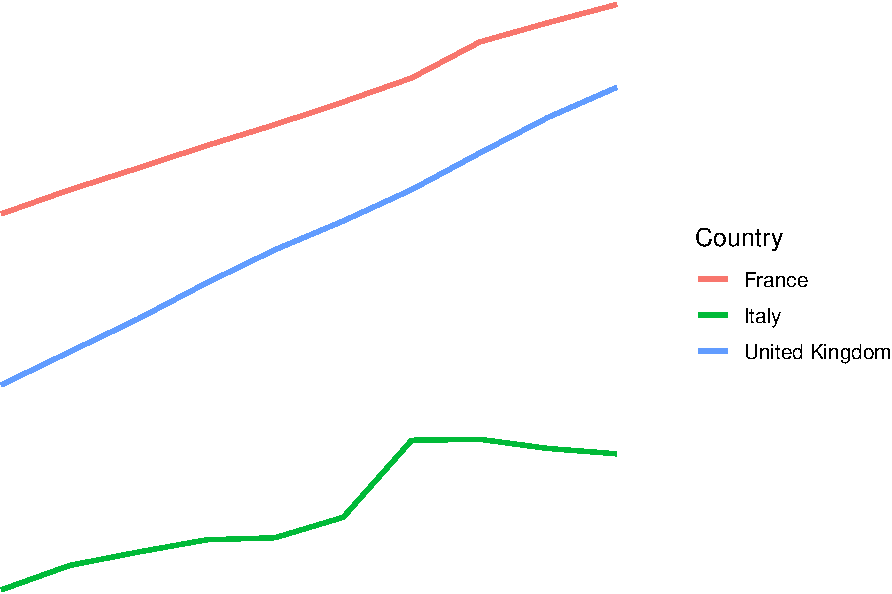
\includegraphics{ScPoEconometrics_files/figure-latex/gather-plot-1} \end{center}

\subsubsection*{\texorpdfstring{Arrange a
\texttt{tibble}}{Arrange a tibble}}\label{arrange-a-tibble}
\addcontentsline{toc}{subsubsection}{Arrange a \texttt{tibble}}

\begin{itemize}
\tightlist
\item
  What are the top/bottom 5 most populated areas?
\end{itemize}

\begin{Shaded}
\begin{Highlighting}[]
\NormalTok{top5 =}\StringTok{ }\NormalTok{tot_pop }\OperatorTok
\StringTok{  }\KeywordTok{arrange}\NormalTok{(}\KeywordTok{desc}\NormalTok{(counts)) }\OperatorTok\StringTok{  }\CommentTok{# arrange in descending order of col `counts`}
\StringTok{  }\KeywordTok{top_n}\NormalTok{(}\DecValTok{5}\NormalTok{)}

\NormalTok{bottom5 =}\StringTok{ }\NormalTok{tot_pop }\OperatorTok
\StringTok{  }\KeywordTok{arrange}\NormalTok{(}\KeywordTok{desc}\NormalTok{(counts)) }\OperatorTok
\StringTok{  }\KeywordTok{top_n}\NormalTok{(}\OperatorTok{-}\DecValTok{5}\NormalTok{)}
\CommentTok{# let's see top 5}
\NormalTok{top5}
\end{Highlighting}
\end{Shaded}

\begin{verbatim}
#OUT> # A tibble: 5 x 3
#OUT>   Country                                                         year    counts
#OUT>   <chr>                                                           <chr>    <int>
#OUT> 1 European Economic Area (EU28  - current composition, plus IS, ~ 2017    5.17e8
#OUT> 2 European Economic Area (EU28  - current composition, plus IS, ~ 2016    5.16e8
#OUT> 3 European Economic Area (EU28  - current composition, plus IS, ~ 2015    5.14e8
#OUT> 4 European Economic Area (EU27 -  before the accession of Croati~ 2017    5.13e8
#OUT> 5 European Economic Area (EU28  - current composition, plus IS, ~ 2014    5.12e8
\end{verbatim}

\begin{Shaded}
\begin{Highlighting}[]
\CommentTok{# and bottom 5}
\NormalTok{bottom5}
\end{Highlighting}
\end{Shaded}

\begin{verbatim}
#OUT> # A tibble: 5 x 3
#OUT>   Country    year  counts
#OUT>   <chr>      <chr>  <int>
#OUT> 1 San Marino 2015   32789
#OUT> 2 San Marino 2014   32520
#OUT> 3 San Marino 2008   32054
#OUT> 4 San Marino 2011   31863
#OUT> 5 San Marino 2009   31269
\end{verbatim}

Now this is not exactly what we wanted. It's always the same country in
both top and bottom, because there are multiple years per country. Let's
compute average population over the last 5 years and rank according to
that:

\begin{Shaded}
\begin{Highlighting}[]
\NormalTok{topbottom =}\StringTok{ }\NormalTok{tot_pop }\OperatorTok
\StringTok{  }\KeywordTok{group_by}\NormalTok{(Country) }\OperatorTok
\StringTok{  }\KeywordTok{filter}\NormalTok{(year }\OperatorTok{>}\StringTok{ }\DecValTok{2012}\NormalTok{) }\OperatorTok
\StringTok{  }\KeywordTok{summarise}\NormalTok{(}\DataTypeTok{mean_count =} \KeywordTok{mean}\NormalTok{(counts)) }\OperatorTok
\StringTok{  }\KeywordTok{arrange}\NormalTok{(}\KeywordTok{desc}\NormalTok{(mean_count))}

\NormalTok{top5 =}\StringTok{ }\NormalTok{topbottom }\OperatorTok\StringTok{ }\KeywordTok{top_n}\NormalTok{(}\DecValTok{5}\NormalTok{)}
\NormalTok{bottom5 =}\StringTok{ }\NormalTok{topbottom }\OperatorTok\StringTok{ }\KeywordTok{top_n}\NormalTok{(}\OperatorTok{-}\DecValTok{5}\NormalTok{)}
\NormalTok{top5}
\end{Highlighting}
\end{Shaded}

\begin{verbatim}
#OUT> # A tibble: 5 x 2
#OUT>   Country                                                             mean_count
#OUT>   <chr>                                                                    <dbl>
#OUT> 1 European Economic Area (EU28  - current composition, plus IS, LI, ~ 514029320 
#OUT> 2 European Economic Area (EU27 -  before the accession of Croatia, p~ 509813491.
#OUT> 3 European Union (current composition)                                508502858.
#OUT> 4 European Union (before the accession of Croatia)                    504287028.
#OUT> 5 European Union (without United Kingdom)                             443638309.
\end{verbatim}

\begin{Shaded}
\begin{Highlighting}[]
\NormalTok{bottom5}
\end{Highlighting}
\end{Shaded}

\begin{verbatim}
#OUT> # A tibble: 5 x 2
#OUT>   Country       mean_count
#OUT>   <chr>              <dbl>
#OUT> 1 Luxembourg       563319.
#OUT> 2 Malta            440467.
#OUT> 3 Iceland          329501.
#OUT> 4 Liechtenstein     37353 
#OUT> 5 San Marino        33014.
\end{verbatim}

That's better!

\subsubsection*{\texorpdfstring{Look for \texttt{NA}s in a
\texttt{tibble}}{Look for NAs in a tibble}}\label{look-for-nas-in-a-tibble}
\addcontentsline{toc}{subsubsection}{Look for \texttt{NA}s in a
\texttt{tibble}}

Sometimes data is \emph{missing}, and \texttt{R} represents it with the
special value \texttt{NA} (not available). It is good to know where in
our dataset we are going to encounter any missing values, so the task
here is: let's produce a table that has three columns:

\begin{enumerate}
\def\labelenumi{\arabic{enumi}.}
\tightlist
\item
  the names of countries with missing data
\item
  how many years of data are missing for each of those
\item
  and the actual years that are missing
\end{enumerate}

\begin{Shaded}
\begin{Highlighting}[]
\NormalTok{missings =}\StringTok{ }\NormalTok{tot_pop }\OperatorTok
\StringTok{  }\KeywordTok{filter}\NormalTok{(}\KeywordTok{is.na}\NormalTok{(counts)) }\OperatorTok\StringTok{ }\CommentTok{# is.na(x) returns TRUE if x is NA}
\StringTok{  }\KeywordTok{group_by}\NormalTok{(Country) }\OperatorTok
\StringTok{  }\KeywordTok{summarise}\NormalTok{(}\DataTypeTok{n_missing =} \KeywordTok{n}\NormalTok{(),}\DataTypeTok{years =} \KeywordTok{paste}\NormalTok{(year,}\DataTypeTok{collapse =} \StringTok{", "}\NormalTok{))}
\NormalTok{knitr}\OperatorTok{:::}\KeywordTok{kable}\NormalTok{(missings)  }\CommentTok{# knitr:::kable makes a nice table}
\end{Highlighting}
\end{Shaded}

\begin{tabular}{l|r|l}
\hline
Country & n\_missing & years\\
\hline
Albania & 2 & 2010, 2012\\
\hline
Andorra & 2 & 2014, 2015\\
\hline
Armenia & 1 & 2014\\
\hline
France (metropolitan) & 4 & 2014, 2015, 2016, 2017\\
\hline
Georgia & 1 & 2013\\
\hline
Monaco & 7 & 2008, 2009, 2010, 2011, 2012, 2013, 2014\\
\hline
Russia & 4 & 2013, 2015, 2016, 2017\\
\hline
San Marino & 1 & 2010\\
\hline
\end{tabular}

\subsubsection*{Males and Females}\label{males-and-females}
\addcontentsline{toc}{subsubsection}{Males and Females}

Let's look at the numbers by male and female population. They are in the
same xls file, but at different cell ranges. Also, I just realised that
the special character \texttt{:} indicates \emph{missing} data. We can
feed that to \texttt{read\_excel} and that will spare us the need to
convert data types afterwards. Let's see:

\begin{Shaded}
\begin{Highlighting}[]
\NormalTok{females_raw =}\StringTok{ }\KeywordTok{read_excel}\NormalTok{(}
                \DataTypeTok{path =} \KeywordTok{system.file}\NormalTok{(}\DataTypeTok{package=}\StringTok{"ScPoEconometrics"}\NormalTok{,}
                                    \StringTok{"datasets"}\NormalTok{,}\StringTok{"demo_gind.xls"}\NormalTok{), }
                \DataTypeTok{sheet=}\StringTok{"Data"}\NormalTok{, }\CommentTok{# which sheet}
                \DataTypeTok{range=}\StringTok{"A141:K200"}\NormalTok{,  }\CommentTok{# which excel cell range to read}
                \DataTypeTok{na=}\StringTok{":"}\NormalTok{ )   }\CommentTok{# missing data indicator}
\KeywordTok{names}\NormalTok{(females_raw)[}\DecValTok{1}\NormalTok{] <-}\StringTok{ "Country"}   \CommentTok{# lets rename the first column}
\NormalTok{females_raw}
\end{Highlighting}
\end{Shaded}

\begin{verbatim}
#OUT> # A tibble: 59 x 11
#OUT>    Country `2008` `2009` `2010` `2011` `2012` `2013` `2014` `2015` `2016` `2017`
#OUT>    <chr>    <dbl>  <dbl>  <dbl>  <dbl>  <dbl>  <dbl>  <dbl>  <dbl>  <dbl>  <dbl>
#OUT>  1 Europe~ 2.56e8 2.57e8 2.58e8 2.58e8 2.58e8 2.59e8 2.60e8 2.60e8 2.61e8 2.61e8
#OUT>  2 Europe~ 2.25e8 2.26e8 2.26e8 2.26e8 2.26e8 2.26e8 2.27e8 2.27e8 2.28e8 2.28e8
#OUT>  3 Europe~ 2.54e8 2.55e8 2.55e8 2.56e8 2.56e8 2.57e8 2.57e8 2.58e8 2.59e8 2.59e8
#OUT>  4 Euro a~ 1.71e8 1.71e8 1.72e8 1.72e8 1.72e8 1.72e8 1.73e8 1.73e8 1.74e8 1.74e8
#OUT>  5 Euro a~ 1.69e8 1.70e8 1.70e8 1.70e8 1.70e8 1.71e8 1.71e8 1.72e8 1.72e8 1.73e8
#OUT>  6 Belgium 5.44e6 5.48e6 5.53e6 5.60e6 5.64e6 5.67e6 5.69e6 5.71e6 5.74e6 5.76e6
#OUT>  7 Bulgar~ 3.86e6 3.83e6 3.81e6 3.78e6 3.76e6 3.74e6 3.72e6 3.70e6 3.68e6 3.65e6
#OUT>  8 Czech ~ 5.28e6 5.31e6 5.33e6 5.34e6 5.35e6 5.35e6 5.35e6 5.36e6 5.37e6 5.38e6
#OUT>  9 Denmark 2.76e6 2.78e6 2.79e6 2.80e6 2.81e6 2.82e6 2.83e6 2.85e6 2.87e6 2.89e6
#OUT> 10 German~ 4.19e7 4.18e7 4.17e7 4.11e7 4.11e7 4.11e7 4.12e7 4.14e7 4.17e7 4.18e7
#OUT> # ... with 49 more rows
\end{verbatim}

You can see that \texttt{R} now correctly read the numbers as such,
after we told it that the \texttt{:} character has the special
\emph{missing} meaning: before, it \emph{coerced} the entire
\texttt{2008} column (for example) to be of type \texttt{chr} after it
hit the first \texttt{:}. We had to manually convert the column back to
\texttt{numeric}, in the process automatically coercing the \texttt{:}s
into \texttt{NA}. Now we addressed that issue directly. Let's also get
the male data in the same way:

\begin{Shaded}
\begin{Highlighting}[]
\NormalTok{males_raw =}\StringTok{ }\KeywordTok{read_excel}\NormalTok{(}
                \DataTypeTok{path =} \KeywordTok{system.file}\NormalTok{(}\DataTypeTok{package=}\StringTok{"ScPoEconometrics"}\NormalTok{,}
                                    \StringTok{"datasets"}\NormalTok{,}\StringTok{"demo_gind.xls"}\NormalTok{), }
                \DataTypeTok{sheet=}\StringTok{"Data"}\NormalTok{, }\CommentTok{# which sheet}
                \DataTypeTok{range=}\StringTok{"A75:K134"}\NormalTok{,  }\CommentTok{# which excel cell range to read}
                \DataTypeTok{na=}\StringTok{":"}\NormalTok{ )   }\CommentTok{# missing data indicator}
\KeywordTok{names}\NormalTok{(males_raw)[}\DecValTok{1}\NormalTok{] <-}\StringTok{ "Country"}   \CommentTok{# lets rename the first column}
\end{Highlighting}
\end{Shaded}

Next step was to \texttt{tidy} up this data, just as before:

\begin{Shaded}
\begin{Highlighting}[]
\NormalTok{females =}\StringTok{ }\KeywordTok{gather}\NormalTok{(females_raw, }\KeywordTok{paste}\NormalTok{(}\DecValTok{2008}\OperatorTok{:}\DecValTok{2017}\NormalTok{),}\DataTypeTok{key=}\StringTok{"year"}\NormalTok{, }\DataTypeTok{value =} \StringTok{"counts"}\NormalTok{)}
\NormalTok{males =}\StringTok{ }\KeywordTok{gather}\NormalTok{(males_raw, }\KeywordTok{paste}\NormalTok{(}\DecValTok{2008}\OperatorTok{:}\DecValTok{2017}\NormalTok{),}\DataTypeTok{key=}\StringTok{"year"}\NormalTok{, }\DataTypeTok{value =} \StringTok{"counts"}\NormalTok{)}
\end{Highlighting}
\end{Shaded}

Let's try to tweak our above plot to show the same data in two separate
panels: one for males and one for females. This is easiest to do with
\texttt{ggplot} if we have all the data in one single
\texttt{data.frame} (or \texttt{tibble}), and marked with a \emph{group
identifier}. Let's first add this to both datasets, and then let's just
combine both into one:

\begin{Shaded}
\begin{Highlighting}[]
\NormalTok{females}\OperatorTok{$}\NormalTok{sex =}\StringTok{ "female"}
\NormalTok{males}\OperatorTok{$}\NormalTok{sex =}\StringTok{ "male"}
\NormalTok{sexes =}\StringTok{ }\KeywordTok{rbind}\NormalTok{(males,females)   }\CommentTok{# "row bind" 2 data.frames}
\NormalTok{sexes}
\end{Highlighting}
\end{Shaded}

\begin{verbatim}
#OUT> # A tibble: 1,180 x 4
#OUT>    Country                                          year     counts sex  
#OUT>    <chr>                                            <chr>     <dbl> <chr>
#OUT>  1 European Union (current composition)             2008  243990548 male 
#OUT>  2 European Union (without United Kingdom)          2008  213826199 male 
#OUT>  3 European Union (before the accession of Croatia) 2008  241913560 male 
#OUT>  4 Euro area (19 countries)                         2008  162516883 male 
#OUT>  5 Euro area (18 countries)                         2008  161029464 male 
#OUT>  6 Belgium                                          2008    5224309 male 
#OUT>  7 Bulgaria                                         2008    3660367 male 
#OUT>  8 Czech Republic                                   2008    5065117 male 
#OUT>  9 Denmark                                          2008    2712666 male 
#OUT> 10 Germany (until 1990 former territory of the FRG) 2008   40274292 male 
#OUT> # ... with 1,170 more rows
\end{verbatim}

Now that we have all the data nice and \texttt{tidy} in a
\texttt{data.frame}, this is a very small change to our previous
plotting code:

\begin{Shaded}
\begin{Highlighting}[]
\NormalTok{sexes }\OperatorTok
\StringTok{  }\KeywordTok{filter}\NormalTok{(Country }\OperatorTok\StringTok{ }\KeywordTok{c}\NormalTok{(}\StringTok{"France"}\NormalTok{,}\StringTok{"United Kingdom"}\NormalTok{,}\StringTok{"Italy"}\NormalTok{)) }\OperatorTok
\StringTok{  }\KeywordTok{mutate}\NormalTok{(}\DataTypeTok{millions =}\NormalTok{ counts }\OperatorTok{/}\StringTok{ }\FloatTok{1e6}\NormalTok{) }\OperatorTok
\StringTok{  }\KeywordTok{ggplot}\NormalTok{(}\DataTypeTok{mapping =} \KeywordTok{aes}\NormalTok{(}\DataTypeTok{x=}\KeywordTok{as.Date}\NormalTok{(year,}\DataTypeTok{format=}\StringTok{"%Y"}\NormalTok{),  }\CommentTok{# convert to `Date`}
                       \DataTypeTok{y=}\NormalTok{millions,}\DataTypeTok{colour=}\NormalTok{Country,}\DataTypeTok{group=}\NormalTok{Country)) }\OperatorTok{+}\StringTok{ }
\StringTok{      }\KeywordTok{geom_line}\NormalTok{() }\OperatorTok{+}
\StringTok{  }\KeywordTok{scale_x_date}\NormalTok{(}\DataTypeTok{name =} \StringTok{"year"}\NormalTok{) }\OperatorTok{+}\StringTok{ }\CommentTok{# rename x axis}
\StringTok{  }\KeywordTok{facet_wrap}\NormalTok{(}\OperatorTok{~}\NormalTok{sex)   }\CommentTok{# make two panels, splitting by groups `sex`}
\end{Highlighting}
\end{Shaded}

\begin{center}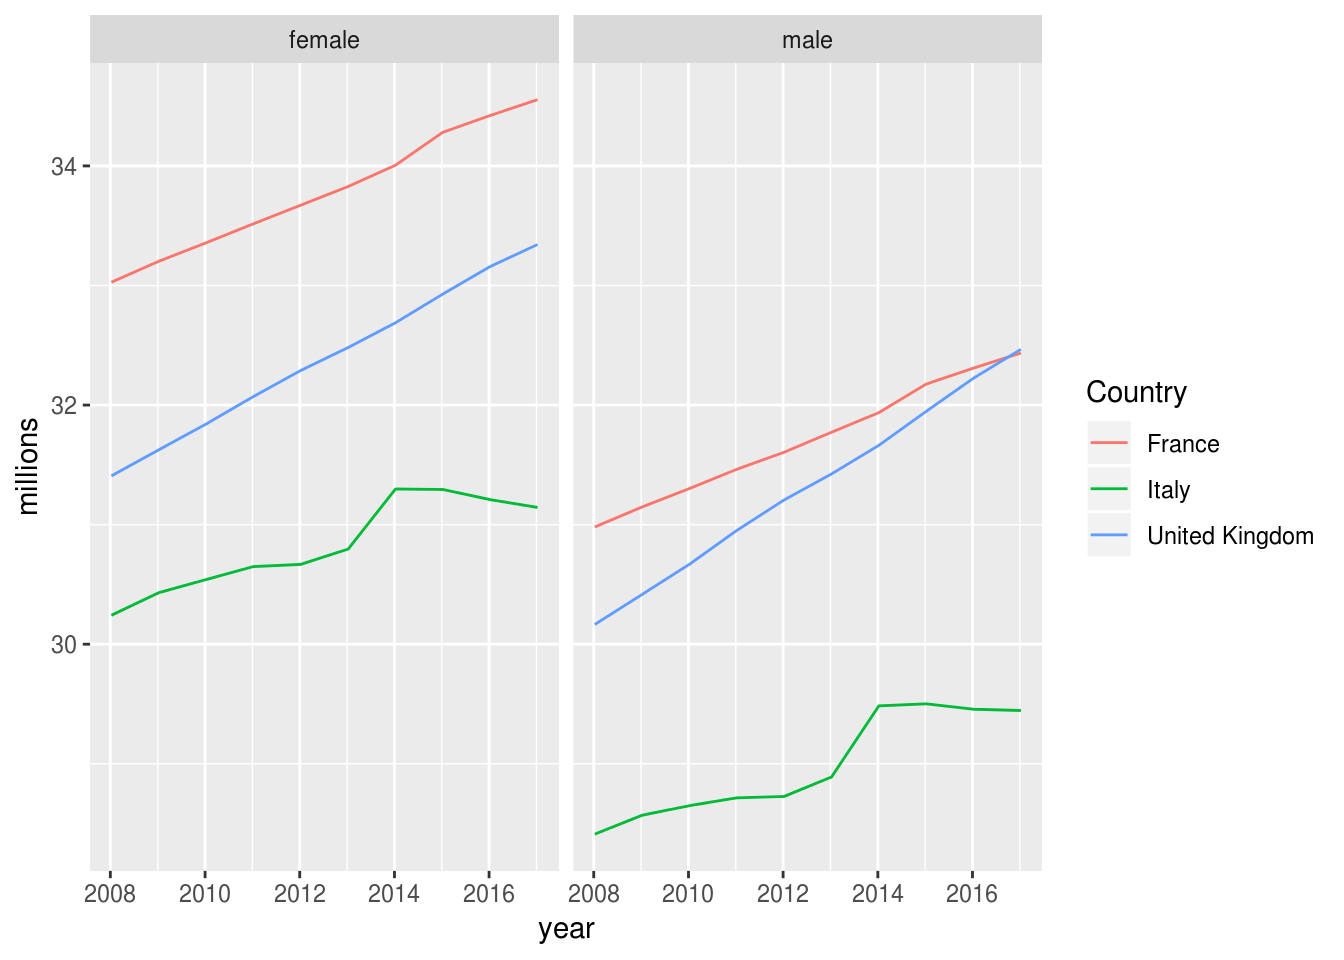
\includegraphics{ScPoEconometrics_files/figure-latex/psexes-1} \end{center}

\subsubsection*{Always Compare to Germany
:-)}\label{always-compare-to-germany--}
\addcontentsline{toc}{subsubsection}{Always Compare to Germany :-)}

How do our three countries compare with respect to the biggest country
in the EU in terms of population? What \emph{fraction} of Germany does
the French population make in any given year, for example?

\begin{Shaded}
\begin{Highlighting}[]
\CommentTok{# remember that the pipe operator %>% takes the }
\CommentTok{# result of the previous operation and passes it}
\CommentTok{# as the *first* argument to the next function call}
\NormalTok{merge_GER <-}\StringTok{ }\NormalTok{tot_pop }\OperatorTok
\StringTok{  }\CommentTok{# 1. subset to countries of interest}
\StringTok{  }\KeywordTok{filter}\NormalTok{(}
\NormalTok{    Country }\OperatorTok\StringTok{ }
\StringTok{      }\KeywordTok{c}\NormalTok{(}\StringTok{"France"}\NormalTok{,}
        \StringTok{"United Kingdom"}\NormalTok{,}
        \StringTok{"Italy"}\NormalTok{)}
\NormalTok{    ) }\OperatorTok
\StringTok{  }\CommentTok{# 2. group data by year}
\StringTok{  }\KeywordTok{group_by}\NormalTok{(year) }\OperatorTok
\StringTok{  }\CommentTok{# 3. add GER's count as new column *by year*}
\StringTok{  }\KeywordTok{left_join}\NormalTok{(}
    \CommentTok{# Germany only}
    \KeywordTok{filter}\NormalTok{(tot_pop,}
\NormalTok{           Country }\OperatorTok\StringTok{ "Germany including former GDR"}\NormalTok{),}
    \CommentTok{# join back in `by year`}
    \DataTypeTok{by=}\StringTok{"year"}\NormalTok{)}
\NormalTok{merge_GER}
\end{Highlighting}
\end{Shaded}

\begin{verbatim}
#OUT> # A tibble: 30 x 5
#OUT> # Groups:   year [10]
#OUT>    Country.x      year  counts.x Country.y                    counts.y
#OUT>    <chr>          <chr>    <int> <chr>                           <int>
#OUT>  1 France         2008  64007193 Germany including former GDR 82217837
#OUT>  2 Italy          2008  58652875 Germany including former GDR 82217837
#OUT>  3 United Kingdom 2008  61571647 Germany including former GDR 82217837
#OUT>  4 France         2009  64350226 Germany including former GDR 82002356
#OUT>  5 Italy          2009  59000586 Germany including former GDR 82002356
#OUT>  6 United Kingdom 2009  62042343 Germany including former GDR 82002356
#OUT>  7 France         2010  64658856 Germany including former GDR 81802257
#OUT>  8 Italy          2010  59190143 Germany including former GDR 81802257
#OUT>  9 United Kingdom 2010  62510197 Germany including former GDR 81802257
#OUT> 10 France         2011  64978721 Germany including former GDR 80222065
#OUT> # ... with 20 more rows
\end{verbatim}

Here you see that the merge (or join) operation labelled \texttt{col.x}
and \texttt{col.y} if both datasets contained a column called
\texttt{col}. Now let's continue to compute what proportion of german
population each country amounts to:

\begin{Shaded}
\begin{Highlighting}[]
\KeywordTok{names}\NormalTok{(merge_GER)[}\DecValTok{1}\NormalTok{] <-}\StringTok{ "Country"}
\NormalTok{merge_GER }\OperatorTok
\StringTok{  }\KeywordTok{mutate}\NormalTok{(}\DataTypeTok{prop_GER =} \DecValTok{100} \OperatorTok{*}\StringTok{ }\NormalTok{counts.x }\OperatorTok{/}\StringTok{ }\NormalTok{counts.y) }\OperatorTok
\StringTok{  }\CommentTok{# 5. plot}
\StringTok{  }\KeywordTok{ggplot}\NormalTok{(}\DataTypeTok{mapping =} 
           \KeywordTok{aes}\NormalTok{(}\DataTypeTok{x =}\NormalTok{ year,}
               \DataTypeTok{y =}\NormalTok{ prop_GER,}
               \DataTypeTok{color =}\NormalTok{ Country,}
               \DataTypeTok{group =}\NormalTok{ Country)) }\OperatorTok{+}\StringTok{ }
\StringTok{  }\KeywordTok{geom_line}\NormalTok{(}\DataTypeTok{size=}\DecValTok{1}\NormalTok{) }\OperatorTok{+}\StringTok{ }
\StringTok{  }\KeywordTok{scale_y_continuous}\NormalTok{(}\StringTok{"percent of German population"}\NormalTok{) }\OperatorTok{+}\StringTok{ }
\StringTok{  }\KeywordTok{theme_bw}\NormalTok{()  }\CommentTok{# new theme for a change?}
\end{Highlighting}
\end{Shaded}

\begin{center}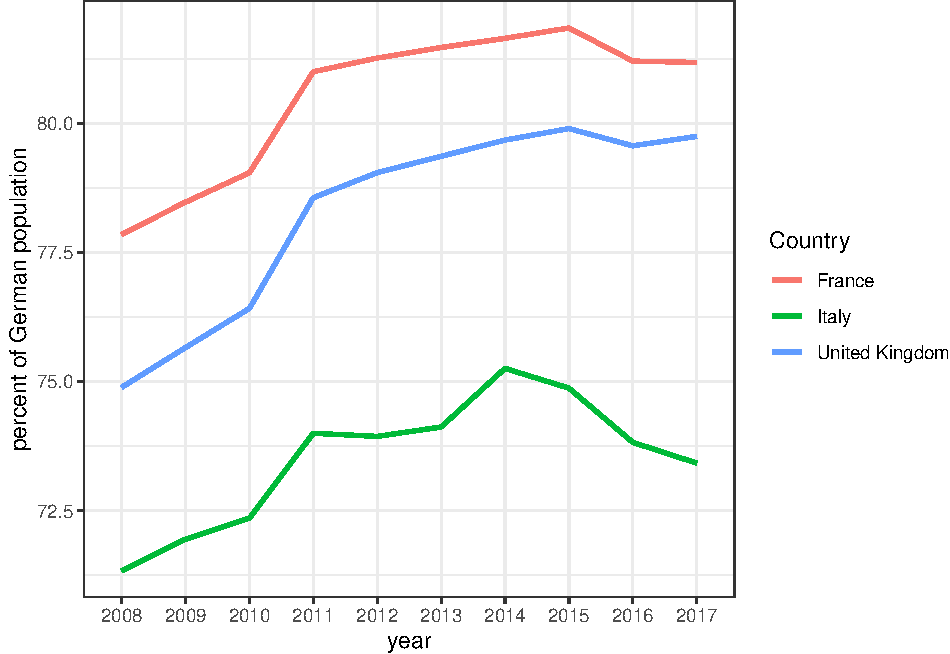
\includegraphics{ScPoEconometrics_files/figure-latex/unnamed-chunk-107-1} \end{center}

\chapter{Linear Regression}\label{linreg}

In this chapter we will learn an additional way how one can represent
the relationship between \emph{outcome}, or \emph{dependent} variable
variable \(y\) and an \emph{explanatory} or \emph{independent} variable
\(x\). We will refer throughout to the graphical representation of a
collection of independent observations on \(x\) and \(y\), i.e., a
\emph{dataset}.

\section{\texorpdfstring{How are \texttt{x} and \texttt{y}
related?}{How are x and y related?}}\label{how-are-x-and-y-related}

\subsection{Data on Cars}\label{data-on-cars}

We will look at the built-in \texttt{cars} dataset. Let's get a view of
this by just typing \texttt{View(cars)} in Rstudio. You can see
something like this:

\begin{verbatim}
#OUT>   speed dist
#OUT> 1     4    2
#OUT> 2     4   10
#OUT> 3     7    4
#OUT> 4     7   22
#OUT> 5     8   16
#OUT> 6     9   10
\end{verbatim}

We have a \texttt{data.frame} with two columns: \texttt{speed} and
\texttt{dist}. Type \texttt{help(cars)} to find out more about the
dataset. There you could read that

\begin{quote}
The data give the speed of cars (mph) and the distances taken to stop
(ft).
\end{quote}

It's good practice to know the extent of a dataset. You could just type

\begin{Shaded}
\begin{Highlighting}[]
\KeywordTok{dim}\NormalTok{(cars)}
\end{Highlighting}
\end{Shaded}

\begin{verbatim}
#OUT> [1] 50  2
\end{verbatim}

to find out that we have 50 rows and 2 columns. A central question that
we want to ask now is the following:

\subsection{\texorpdfstring{How are \texttt{speed} and \texttt{dist}
related?}{How are speed and dist related?}}\label{how-are-speed-and-dist-related}

The simplest way to start is to plot the data. Remembering that we view
each row of a data.frame as an observation, we could just label one axis
of a graph \texttt{speed}, and the other one \texttt{dist}, and go
through our table above row by row. We just have to read off the x/y
coordinates and mark them in the graph. In \texttt{R}:

\begin{Shaded}
\begin{Highlighting}[]
\KeywordTok{plot}\NormalTok{(dist }\OperatorTok{~}\StringTok{ }\NormalTok{speed, }\DataTypeTok{data =}\NormalTok{ cars,}
     \DataTypeTok{xlab =} \StringTok{"Speed (in Miles Per Hour)"}\NormalTok{,}
     \DataTypeTok{ylab =} \StringTok{"Stopping Distance (in Feet)"}\NormalTok{,}
     \DataTypeTok{main =} \StringTok{"Stopping Distance vs Speed"}\NormalTok{,}
     \DataTypeTok{pch  =} \DecValTok{20}\NormalTok{,}
     \DataTypeTok{cex  =} \DecValTok{2}\NormalTok{,}
     \DataTypeTok{col  =} \StringTok{"red"}\NormalTok{)}
\end{Highlighting}
\end{Shaded}

\begin{center}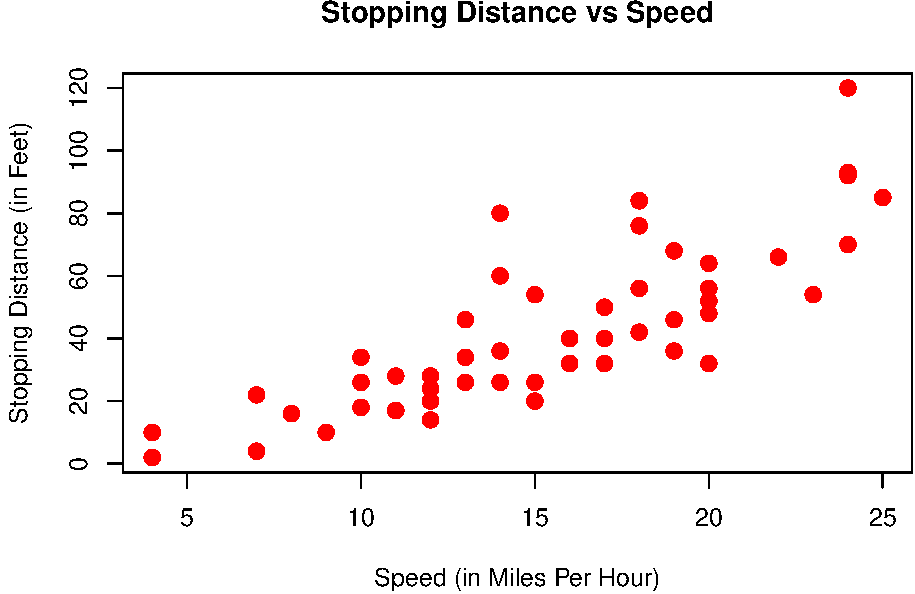
\includegraphics{ScPoEconometrics_files/figure-latex/unnamed-chunk-110-1} \end{center}

Here, each dot represents one observation. In this case, one particular
measurement \texttt{speed} and \texttt{dist} for a car. Now, again:

\begin{note}
How are \texttt{speed} and \texttt{dist} related? How could one best
\emph{summarize} this relationship?
\end{note}

 One thing we could do, is draw a straight line through this
scatterplot, like so:

\begin{Shaded}
\begin{Highlighting}[]
\KeywordTok{plot}\NormalTok{(dist }\OperatorTok{~}\StringTok{ }\NormalTok{speed, }\DataTypeTok{data =}\NormalTok{ cars,}
     \DataTypeTok{xlab =} \StringTok{"Speed (in Miles Per Hour)"}\NormalTok{,}
     \DataTypeTok{ylab =} \StringTok{"Stopping Distance (in Feet)"}\NormalTok{,}
     \DataTypeTok{main =} \StringTok{"Stopping Distance vs Speed"}\NormalTok{,}
     \DataTypeTok{pch  =} \DecValTok{20}\NormalTok{,}
     \DataTypeTok{cex  =} \DecValTok{2}\NormalTok{,}
     \DataTypeTok{col  =} \StringTok{"red"}\NormalTok{)}
\KeywordTok{abline}\NormalTok{(}\DataTypeTok{a =} \DecValTok{60}\NormalTok{,}\DataTypeTok{b =} \DecValTok{0}\NormalTok{,}\DataTypeTok{lw=}\DecValTok{3}\NormalTok{)}
\end{Highlighting}
\end{Shaded}

\begin{center}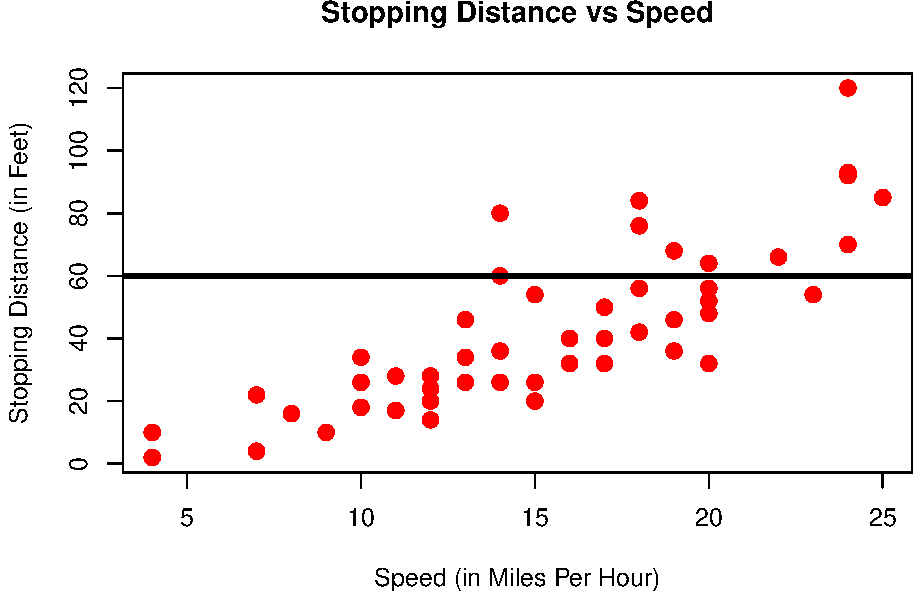
\includegraphics{ScPoEconometrics_files/figure-latex/unnamed-chunk-112-1} \end{center}

Now that doesn't seem a particularly \emph{good} way to summarize the
relationship. Clearly, a \emph{better} line would be not be flat, but
have a \emph{slope}, i.e.~go upwards:

\begin{center}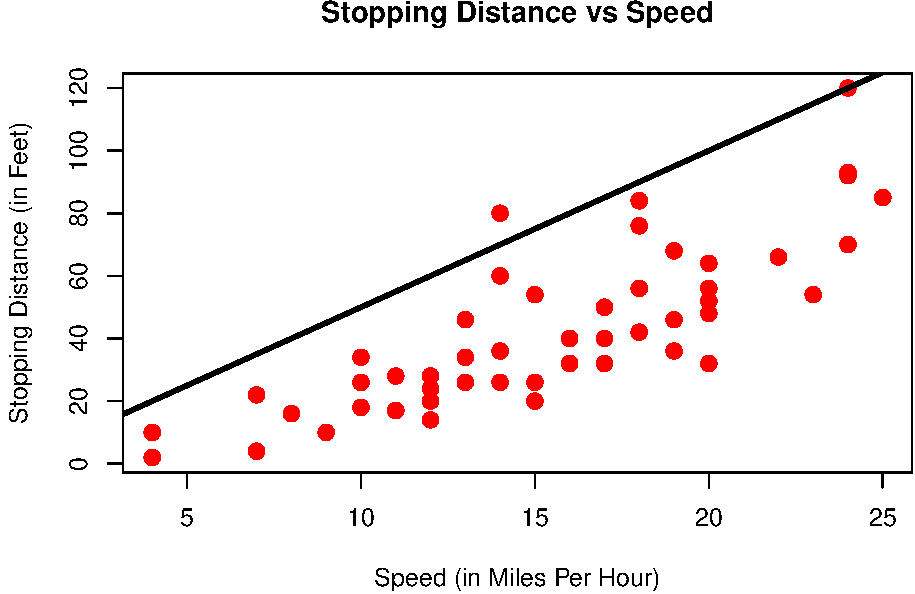
\includegraphics{ScPoEconometrics_files/figure-latex/unnamed-chunk-113-1} \end{center}

That is slightly better. However, the line seems at too high a level -
the point at which it crosses the y-axis is called the \emph{intercept};
and it's too high. We just learned how to represent a \emph{line},
i.e.~with two numbers called \emph{intercept} and \emph{slope}. Let's
write down a simple formula which represents a line where some outcome
\(z\) is related to a variable \(x\):

\begin{equation}
z = b_0 + b_1 x \label{eq:bline}
\end{equation}

Here \(b_0\) represents the value of the intercept (i.e. \(z\) when
\(x=0\)), and \(b_1\) is the value of the slope. The question for us is
now: How to choose the number \(b_0\) and \(b_1\) such that the result
is the \textbf{good} line?

\subsection{Choosing the Best Line}\label{choosing-the-best-line}

In order to be able to reason about good or bad line, we need to denote
the \emph{output} of equation \eqref{eq:bline}. We call the value
\(\hat{y}_i\) the \emph{predicted value} for obseration \(i\), after
having chosen some particular values \(b_0\) and \(b_1\):

\begin{equation}
\hat{y}_i = b_0 + b_1 x_i \label{eq:abline-pred}
\end{equation}

In general it is likely that we won't be able to choose \(b_0\) and
\(b_1\) in such as way as to provide a perfect prediction, i.e.~one
where \(\hat{y}_i = y_i\) for all \(i\). That is, we expect to make an
\emph{error} in our prediction \(\hat{y}_i\), so let's denote this value
\(e_i\). If we acknowlegdge that we will make errors, let's at least
make them as small as possible! Exactly this is going to be our task
now.

Suppose we have the following set of 9 observations on \texttt{x} and
\texttt{y}, and we put the \emph{best} straight line into it, that we
can think of. It would look like this:

\begin{figure}

{\centering 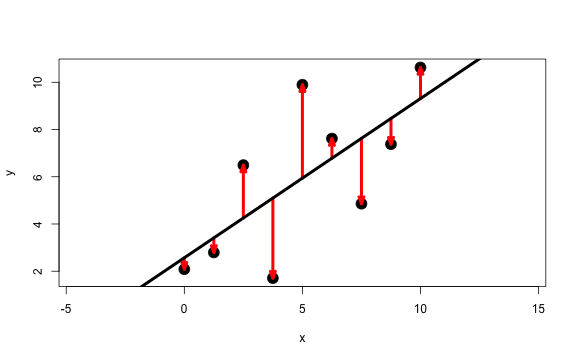
\includegraphics{ScPoEconometrics_files/figure-latex/line-arrows-1} 

}

\caption{The best line and its errors}\label{fig:line-arrows}
\end{figure}

Here, the red arrows indicate the \textbf{distance} between the
prediction (i.e.~the black line) to each data point, in other words,
each arrow is a particular \(e_i\). An upward pointing arrow indicates a
positive value of a particular \(e_i\), and vice versa for downward
pointing arrows. The erros are also called \emph{residuals}, which comes
from the way can write the equation for this relationship between two
particular values \((y_i,x_i)\) belonging to observation \(i\):

\begin{equation}
y_i = b_0 + b_1 x_i + e_i \label{eq:abline}
\end{equation}

You realize of course that \(\hat{y}_i = y_i - e_i\), which just means
that our prediction is the observed value \(y_i\) minus any error
\(e_i\) we make. In other words, \(e_i\) is what is left to be explained
on top of the line \(b_0 + b_1 x_i\), hence, it's a residual to explain
\(y_i\). Here are \(y,\hat{y}\) and the resulting \(e\) which are
plotted in figure \ref{fig:line-arrows}:

\begin{tabular}{c|c|c|c}
\hline
x & y & y\_hat & error\\
\hline
0.00 & 2.09 & 2.57 & -0.48\\
\hline
1.25 & 2.79 & 3.41 & -0.62\\
\hline
2.50 & 6.49 & 4.25 & 2.24\\
\hline
3.75 & 1.71 & 5.10 & -3.39\\
\hline
5.00 & 9.89 & 5.94 & 3.95\\
\hline
6.25 & 7.62 & 6.78 & 0.83\\
\hline
7.50 & 4.86 & 7.63 & -2.77\\
\hline
8.75 & 7.38 & 8.47 & -1.09\\
\hline
10.00 & 10.63 & 9.31 & 1.32\\
\hline
\end{tabular}

If our line was a \textbf{perfect fit} to the data, all \(e_i = 0\), and
the column \texttt{error} would display \texttt{0} for each row - there
would be no errors at all. (All points in figure \ref{fig:line-arrows}
would perfectly line up on a straight line).

Now, back to our claim that this particular line is the \emph{best}
line. What exactly characterizes this best line? We now come back to
what we said above - \emph{how to make the errors as small as possible}?
Keeping in mind that each residual \(e_i\) is \(y_i - \hat{y}_i\), we
have the following minization problem to solve:

\begin{align}
e_i & = y_i - \hat{y}_i = y_i - \underbrace{\left(b_0 + b_1 x_i\right)}_\text{prediction}\\
e_1^2 + \dots + e_N^2 &= \sum_{i=1}^N e_i^2 \equiv \text{SSR}(b_0,b_1) \\
(b_0,b_1) &= \arg \min_{\text{int},\text{slope}} \sum_{i=1}^N \left[y_i - \left(\text{int} + \text{slope } x_i\right)\right]^2 \label{eq:ols-min}
\end{align}

\begin{warning}
The best line chooses \(b_0\) and \(b_1\) so as to minimize the sum of
\textbf{squared residuals} (SSR).
\end{warning}

 Wait a moment, why \emph{squared} residuals? This is easy to
understand: suppose that instead, we wanted to just make the \emph{sum}
of the arrows in figure \ref{fig:line-arrows} as small as possible (that
is, no squares). Choosing our line to make this number small would not
give a particularly good representation of the data -- given that errors
of opposite sign and equal magnitude offset, we could have very long
arrows (but of opposite signs), and a poor resulting line. Squaring each
error avoids this (because now negative errors get positive values!)

\begin{figure}

{\centering 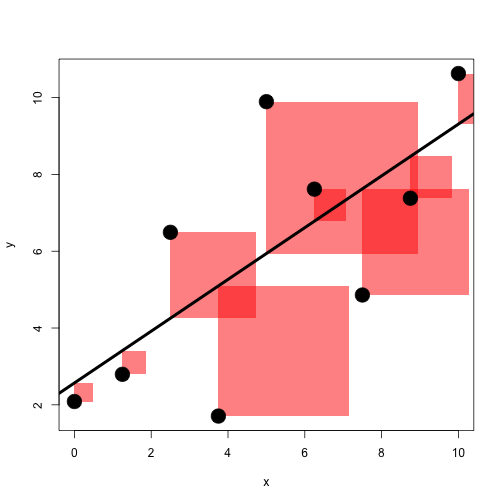
\includegraphics{ScPoEconometrics_files/figure-latex/line-squares-1} 

}

\caption{The best line and its SQUARED errors}\label{fig:line-squares}
\end{figure}

We illustrate this in figure \ref{fig:line-squares}. This is the same
data as in figure \ref{fig:line-arrows}, but instead of arrows of length
\(e_i\) for each observation \(i\), now we draw a square with side
\(e_i\), i.e.~an area of \(e_i^2\). We have two apps for you at this
point, one where you have to try and find the best line by choosing
\(b_0\) and \(b_1\), only focusing on the sum of errors (and not their
square), and a second one focusing on squared errors:

\begin{Shaded}
\begin{Highlighting}[]
\KeywordTok{library}\NormalTok{(ScPoEconometrics)}
\KeywordTok{launchApp}\NormalTok{(}\StringTok{"reg_simple_arrows"}\NormalTok{)}
\KeywordTok{launchApp}\NormalTok{(}\StringTok{"reg_simple"}\NormalTok{) }\CommentTok{# with squared errors}
\KeywordTok{launchApp}\NormalTok{(}\StringTok{"SSR_cone"}\NormalTok{) }\CommentTok{# visualize the minimzation problem from above!}
\end{Highlighting}
\end{Shaded}

Most of our \texttt{apps} have an associated \texttt{about} document,
which gives extra information and explanations. After you have looked at
all three apps, we invite you thus to have a look at the associated
explainers by typing

\begin{Shaded}
\begin{Highlighting}[]
\KeywordTok{aboutApp}\NormalTok{(}\StringTok{"reg_simple_arrows"}\NormalTok{)}
\KeywordTok{aboutApp}\NormalTok{(}\StringTok{"reg_simple"}\NormalTok{) }
\KeywordTok{aboutApp}\NormalTok{(}\StringTok{"SSR_cone"}\NormalTok{) }
\end{Highlighting}
\end{Shaded}

\section{Ordinary Least Squares (OLS) Estimator}\label{OLS}

The method to compute (or \emph{estimate}) \(b_0\) and \(b_1\) we
illustrated above is called \emph{Ordinary Least Squares}, or OLS.
\(b_0\) and \(b_1\) are therefore also often called the \emph{OLS
coefficients}. By solving problem \eqref{eq:ols-min} one can derive an
explicit formula for them:

\begin{equation}
b_1 = \frac{cov(x,y)}{var(x)},  \label{eq:beta1hat}
\end{equation}

i.e.~the estimate of the slope coefficient is the covariance between
\(x\) and \(y\) divided by the variance of \(x\), both computed from our
sample of data. With \(b_1\) in hand, we can get the estimate for the
intercept as

\begin{equation}
b_0 = \bar{y} - b_1 \bar{x}.  \label{eq:beta0hat}
\end{equation}

where \(\bar{z}\) denotes the sample mean of variable \(z\). The
interpretation of the OLS slope coefficient \(b_1\) is as follows. Given
a line as in \(y = b_0 + b_1 x\),

\begin{itemize}
\tightlist
\item
  \(b_1 = \frac{d y}{d x}\) measures the change in \(y\) resulting from
  a one unit change in \(x\)
\item
  For example, if \(y\) is wage and \(x\) is years of education, \(b_1\)
  would measure the effect of an additional year of education on wages.
\end{itemize}

There is an alternative representation for the OLS slope coefficient
which relates to the \emph{correlation coefficient} \(r\). Remember from
section \ref{summarize-two} that \(r = \frac{cov(x,y)}{s_x s_y}\), where
\(s_z\) is the standard deviation of variable \(z\). With this in hand,
we can derive the OLS slope coefficient as

\begin{align}
b_1 &= \frac{cov(x,y)}{var(x)}\\
    &= \frac{cov(x,y)}{s_x s_x} \\
    &= r\frac{s_y}{s_x} \label{eq:beta1-r}
\end{align}

In other words, the slope coefficient is equal to the correlation
coefficient \(r\) times the ratio of standard deviations of \(y\) and
\(x\).

\subsection{Linear Regression without
Regressor}\label{linear-regression-without-regressor}

There are several important special cases for the linear regression
introduced above. Let's start with the most obvious one: What is the
meaning of running a regression \emph{without any regressor},
i.e.~without a \(x\)? Our line becomes very simple. Instead of
\eqref{eq:bline}, we get

\begin{equation}
y = b_0. \label{eq:b0line}
\end{equation}

This means that our minization problem in \eqref{eq:ols-min} \emph{also}
becomes very simple: We only have to choose \(b_0\)! We have

\[
b_0 = \arg\min_{\text{int}} \sum_{i=1}^N \left[y_i - \text{int}\right]^2,
\] which is a quadratic equation with a unique optimum such that \[
b_0 = \frac{1}{N} \sum_{i=1}^N y_i = \overline{y}.
\]

\begin{tip}
Least Squares \textbf{without regressor} \(x\) estimates the sample mean
of the outcome variable \(y\), i.e.~it produces \(\overline{y}\).
\end{tip}

\subsection{Regression without an
Intercept}\label{regression-without-an-intercept}

We follow the same logic here, just that we miss another bit from our
initial equation and the minimisation problem in \eqref{eq:ols-min} now
becomes:

\begin{align}
b_1 &= \arg\min_{\text{slope}} \sum_{i=1}^N \left[y_i - \text{slope } x_i \right]^2\\
\mapsto b_1 &= \frac{\frac{1}{N}\sum_{i=1}^N x_i y_i}{\frac{1}{N}\sum_{i=1}^N x_i^2} = \frac{\bar{x} \bar{y}}{\overline{x^2}} \label{eq:b1line}
\end{align}

\begin{tip}
Least Squares \textbf{without intercept} (i.e.~with \(b_0=0\)) is a line
that passes through the origin.
\end{tip}

In this case we only get to choose the slope \(b_1\) of this anchored
line.\footnote{This slope is related to the angle between vectors
  \(\mathbf{a} = (\overline{x},\overline{y})\), and
  \(\mathbf{b} = (\overline{x},0)\). Hence, it's related to the
  \href{https://en.wikipedia.org/wiki/Scalar_projection}{scalar
  projection} of \(\mathbf{a}\) on \(\mathbf{b}\).} You should now try
out both of those restrictions on our linear model by spending some time
with

\begin{Shaded}
\begin{Highlighting}[]
\KeywordTok{launchApp}\NormalTok{(}\StringTok{"reg_constrained"}\NormalTok{)}
\end{Highlighting}
\end{Shaded}

\subsection{Centering A Regression}\label{centering-a-regression}

By \emph{centering} or \emph{demeaning} a regression, we mean to
substract from both \(y\) and \(x\) their respective averages to obtain
\(\tilde{y}_i = y_i - \bar{y}\) and \(\tilde{x}_i = x_i - \bar{x}\). We
then run a regression \emph{without intercept} as above. That is, we use
\(\tilde{x}_i,\tilde{y}_i\) instead of \(x_i,y_i\) in \eqref{eq:b1line} to
obtain our slope estimate \(b_1\):

\begin{align}
b_1 &= \frac{\frac{1}{N}\sum_{i=1}^N \tilde{x}_i \tilde{y}_i}{\frac{1}{N}\sum_{i=1}^N \tilde{x}_i^2}\\
    &= \frac{\frac{1}{N}\sum_{i=1}^N (x_i - \bar{x}) (y_i - \bar{y})}{\frac{1}{N}\sum_{i=1}^N (x_i - \bar{x})^2} \\
    &= \frac{cov(x,y)}{var(x)}
    \label{eq:bline-centered}
\end{align}

This last expression is \emph{identical} to the one in
\eqref{eq:beta1hat}! It's the standard OLS estimate for the slope
coefficient. We note the following:

\begin{tip}
Adding a constant to a regression produces the same result as centering
all variables and estimating without intercept. So, unless all variables
are centered, \textbf{always} include an intercept in the regression.
\end{tip}

 To get a better feel for what is going on here, you can try this out
now by yourself by typing:

\begin{Shaded}
\begin{Highlighting}[]
\KeywordTok{launchApp}\NormalTok{(}\StringTok{"demeaned_reg"}\NormalTok{)}
\end{Highlighting}
\end{Shaded}

\subsection{Standardizing A Regression}\label{reg-standard}

\emph{Standardizing} a variable \(z\) means to demean as above, but in
addition to divide the demeaned value by its own standard deviation.
Similarly to what we did above for \emph{centering}, we define
transformed variables \(\breve{y}_i = \frac{y_i-\bar{y}}{\sigma_y}\) and
\(\breve{x}_i = \frac{x_i-\bar{x}}{\sigma_x}\) where \(\sigma_z\) is the
standard deviation of variable \(z\). From here on, you should by now be
used to what comes next! As above, we use \(\breve{x}_i,\breve{y}_i\)
instead of \(x_i,y_i\) in \eqref{eq:b1line} to this time obtain:

\begin{align}
b_1 &= \frac{\frac{1}{N}\sum_{i=1}^N \breve{x}_i \breve{y}_i}{\frac{1}{N}\sum_{i=1}^N \breve{x}_i^2}\\
    &= \frac{\frac{1}{N}\sum_{i=1}^N \frac{x_i - \bar{x}}{\sigma_x} \frac{y_i - \bar{y}}{\sigma_y}}{\frac{1}{N}\sum_{i=1}^N \left(\frac{x_i - \bar{x}}{\sigma_x}\right)^2} \\
    &= \frac{Cov(x,y)}{\sigma_x \sigma_y} \\
    &= Corr(x,y)  \label{eq:bline-standardized}
\end{align}

\begin{tip}
After we standardize both \(y\) and \(x\), the slope coefficient \(b_1\)
in the regression without intercept is equal to the \textbf{correlation
coefficient}.
\end{tip}

 And also for this case we have a practical application for you. Just
type this and play around with the app for a little while!

\begin{Shaded}
\begin{Highlighting}[]
\KeywordTok{launchApp}\NormalTok{(}\StringTok{"reg_standardized"}\NormalTok{)}
\end{Highlighting}
\end{Shaded}

\section{Predictions and Residuals}\label{pred-resids}

Now we want to ask how our residuals \(e_i\) relate to the prediction
\(\hat{y_i}\). Let us first think about the average of all predictions
\(\hat{y_i}\), i.e.~the number \(\frac{1}{N} \sum_{i=1}^N \hat{y_i}\).
Let's just take \eqref{eq:abline-pred} and plug this into this average, so
that we get

\begin{align}
\frac{1}{N} \sum_{i=1}^N \hat{y_i} &= \frac{1}{N} \sum_{i=1}^N b_0 + b_1 x_i \\
&= b_0 + b_1  \frac{1}{N} \sum_{i=1}^N x_i \\
&= b_0 + b_1  \bar{x} \\
\end{align}

But that last line is just equal to the formula for the OLS intercept
\eqref{eq:beta0hat}, \(b_0 = \bar{y} - b_1 \bar{x}\)! That means of course
that

\[
\frac{1}{N} \sum_{i=1}^N \hat{y_i}  = b_0 + b_1  \bar{x} = \bar{y}
\] in other words:

\begin{tip}
The average of our predictions \(\hat{y_i}\) is identically equal to the
mean of the outcome \(y\). This implies that the average of the
residuals is equal to zero.
\end{tip}

 Related to this result, we can show that the prediction \(\hat{y}\) and
the residuals are \emph{uncorrelated}, something that is often called
\textbf{orthogonality} between \(\hat{y}_i\) and \(e_i\). We would write
this as

\begin{align}
Cov(\hat{y},e) &=\frac{1}{N} \sum_{i=1}^N (\hat{y}_i-\bar{y})(e_i-\bar{e}) =   \frac{1}{N} \sum_{i=1}^N (\hat{y}_i-\bar{y})e_i \\
&=  \frac{1}{N} \sum_{i=1}^N \hat{y}_i e_i-\bar{y} \frac{1}{N} \sum_{i=1}^N e_i = 0
\end{align}

It's useful to bring back the sample data which generate figure
\ref{fig:line-arrows} at this point in order to verify these claims:

\begin{verbatim}
#OUT>       y y_hat error
#OUT> 1  2.09  2.57 -0.48
#OUT> 2  2.79  3.41 -0.62
#OUT> 3  6.49  4.25  2.24
#OUT> 4  1.71  5.10 -3.39
#OUT> 5  9.89  5.94  3.95
#OUT> 6  7.62  6.78  0.83
#OUT> 7  4.86  7.63 -2.77
#OUT> 8  7.38  8.47 -1.09
#OUT> 9 10.63  9.31  1.32
\end{verbatim}

Let's check that these claims are true in this sample of data. We want
that

\begin{enumerate}
\def\labelenumi{\arabic{enumi}.}
\tightlist
\item
  The average of \(\hat{y}_i\) to be the same as the mean of \(y\)
\item
  The average of the errors should be zero.
\item
  Prediction and errors should be uncorrelated.
\end{enumerate}

\begin{Shaded}
\begin{Highlighting}[]
\CommentTok{# 1.}
\KeywordTok{all.equal}\NormalTok{(}\KeywordTok{mean}\NormalTok{(ss}\OperatorTok{$}\NormalTok{error), }\DecValTok{0}\NormalTok{)}
\end{Highlighting}
\end{Shaded}

\begin{verbatim}
#OUT> [1] TRUE
\end{verbatim}

\begin{Shaded}
\begin{Highlighting}[]
\CommentTok{# 2.}
\KeywordTok{all.equal}\NormalTok{(}\KeywordTok{mean}\NormalTok{(ss}\OperatorTok{$}\NormalTok{y_hat), }\KeywordTok{mean}\NormalTok{(ss}\OperatorTok{$}\NormalTok{y))}
\end{Highlighting}
\end{Shaded}

\begin{verbatim}
#OUT> [1] TRUE
\end{verbatim}

\begin{Shaded}
\begin{Highlighting}[]
\CommentTok{# 3.}
\KeywordTok{all.equal}\NormalTok{(}\KeywordTok{cov}\NormalTok{(ss}\OperatorTok{$}\NormalTok{error,ss}\OperatorTok{$}\NormalTok{y_hat), }\DecValTok{0}\NormalTok{)}
\end{Highlighting}
\end{Shaded}

\begin{verbatim}
#OUT> [1] TRUE
\end{verbatim}

So indeed we can confirm this result with our test dataset. Great!

\section{Correlation, Covariance and
Linearity}\label{correlation-covariance-and-linearity}

It is important to keep in mind that Correlation and Covariance relate
to a \emph{linear} relationship between \texttt{x} and \texttt{y}. Given
how the regression line is estimated by OLS (see just above), you can
see that the regression line inherits this property from the Covariance.
A famous exercise by Francis Anscombe (1973) illustrates this by
constructing 4 different datasets which all have identical
\textbf{linear} statistics: mean, variance, correlation and regression
line \emph{are identical}. However, the usefulness of the statistics to
describe the relationship in the data is not clear.

\begin{center}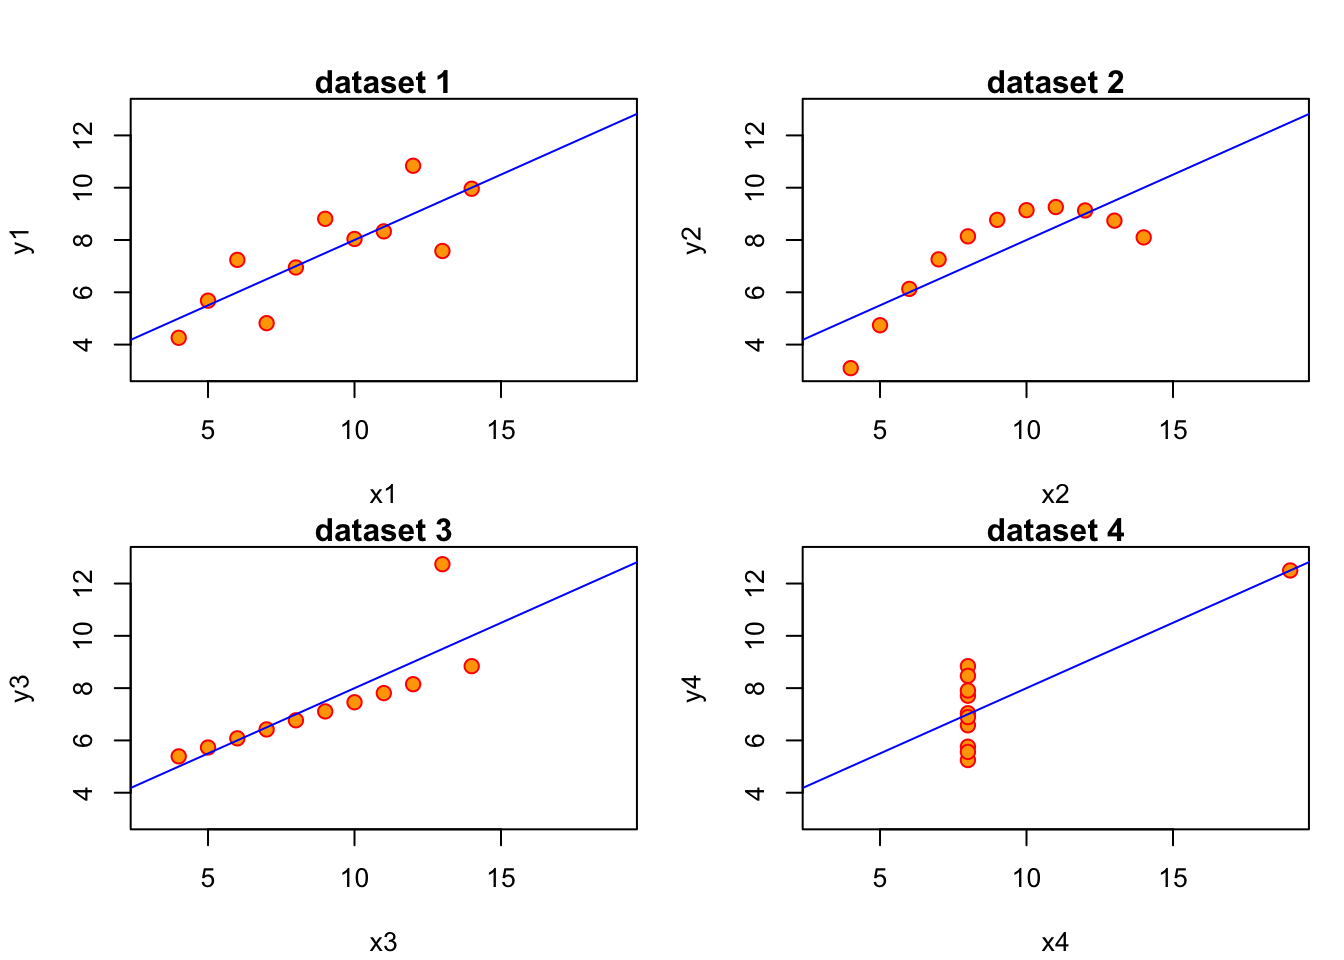
\includegraphics{ScPoEconometrics_files/figure-latex/unnamed-chunk-129-1} \end{center}

The important lesson from this example is the following:

\begin{warning}
Always \textbf{visually inspect} your data, and don't rely exclusively
on summary statistics like \emph{mean, variance, correlation and
regression line}. All of those assume a \textbf{linear} relationship
between the variables in your data.
\end{warning}

 The mission of Anscombe has been continued recently. As a result of
this we can have a look at the \texttt{datasauRus} package, which
pursues Anscbombe's idea through a multitude of funny data sets, all
with the same linear statistics. Don't just compute the covariance, or
you might actually end up looking at a Dinosaur! What? Type this to find
out:

\begin{Shaded}
\begin{Highlighting}[]
\KeywordTok{launchApp}\NormalTok{(}\StringTok{"datasaurus"}\NormalTok{)}
\KeywordTok{aboutApp}\NormalTok{(}\StringTok{"datasaurus"}\NormalTok{)}
\end{Highlighting}
\end{Shaded}

\subsection{Non-Linear Relationships in
Data}\label{non-linear-relationships-in-data}

Suppose our data now looks like this:

\begin{center}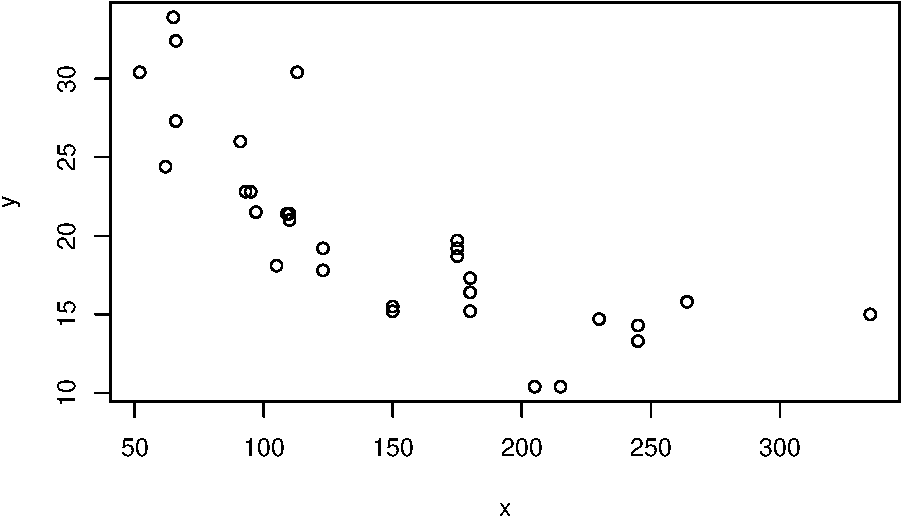
\includegraphics{ScPoEconometrics_files/figure-latex/non-line-cars-1} \end{center}

Putting our previous \emph{best line} defined in equation
\eqref{eq:abline} as \(y = b_0 + b_1 x + e\), we get something like this:

\begin{figure}

{\centering 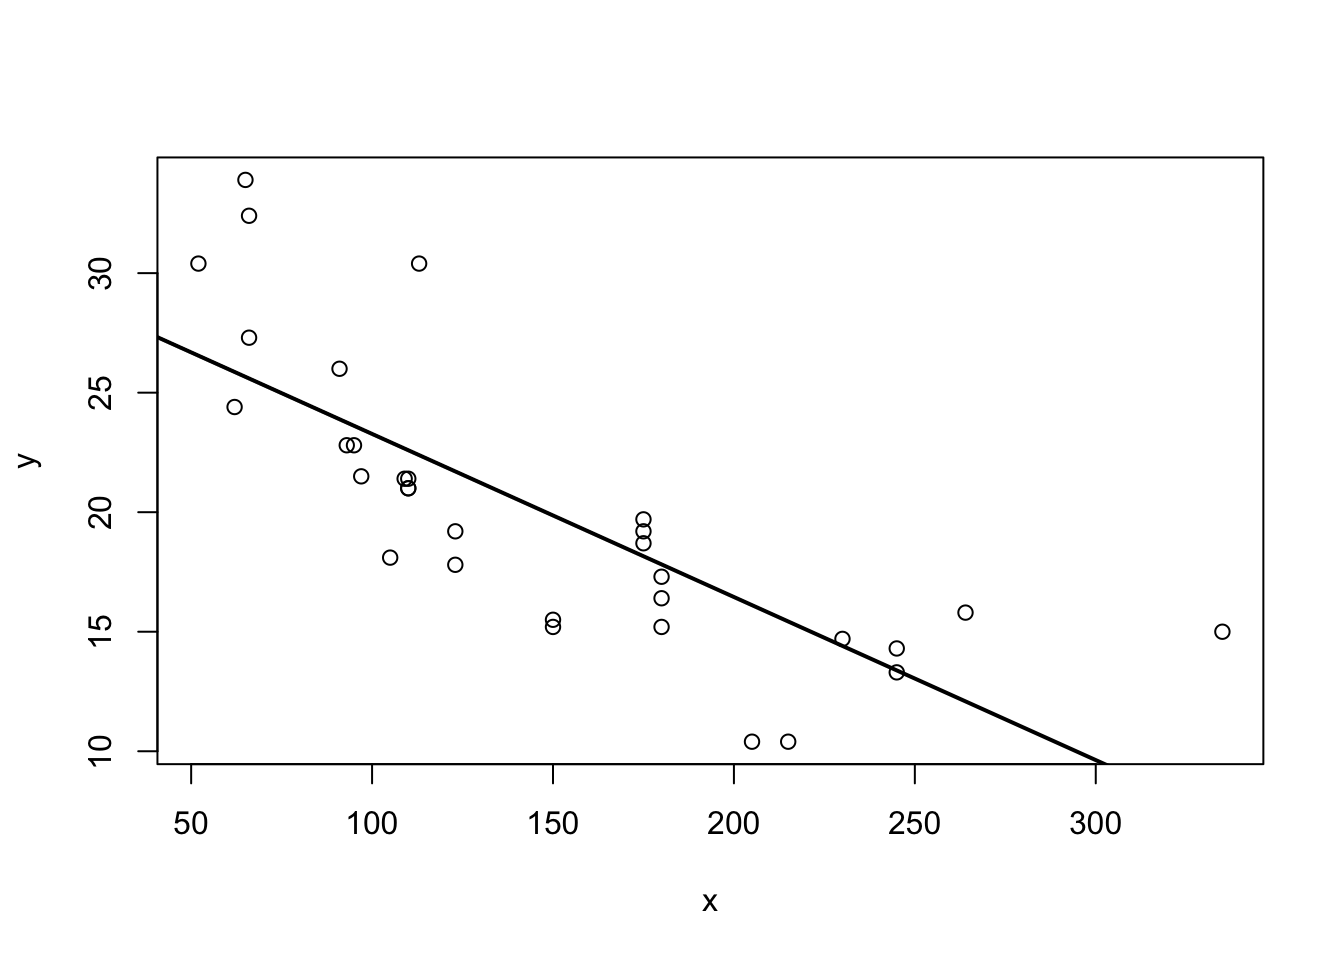
\includegraphics{ScPoEconometrics_files/figure-latex/non-line-cars-ols-1} 

}

\caption{Best line with non-linear data?}\label{fig:non-line-cars-ols}
\end{figure}

Somehow when looking at \ref{fig:non-line-cars-ols} one is not totally
convinced that the straight line is a good summary of this relationship.
For values \(x\in[50,120]\) the line seems to low, then again too high,
and it completely misses the right boundary. It's easy to address this
shortcoming by including \emph{higher order terms} of an explanatory
variable. We would modify \eqref{eq:abline} to read now

\begin{equation}
y_i = b_0 + b_1 x_i + b_2 x_i^2 + e_i \label{eq:abline2}
\end{equation}

This is a special case of \emph{multiple regression}, which we will talk
about in chapter \ref{multiple-reg}. You can see that there are
\emph{multiple} slope coefficients. For now, let's just see how this
performs:

\begin{figure}

{\centering 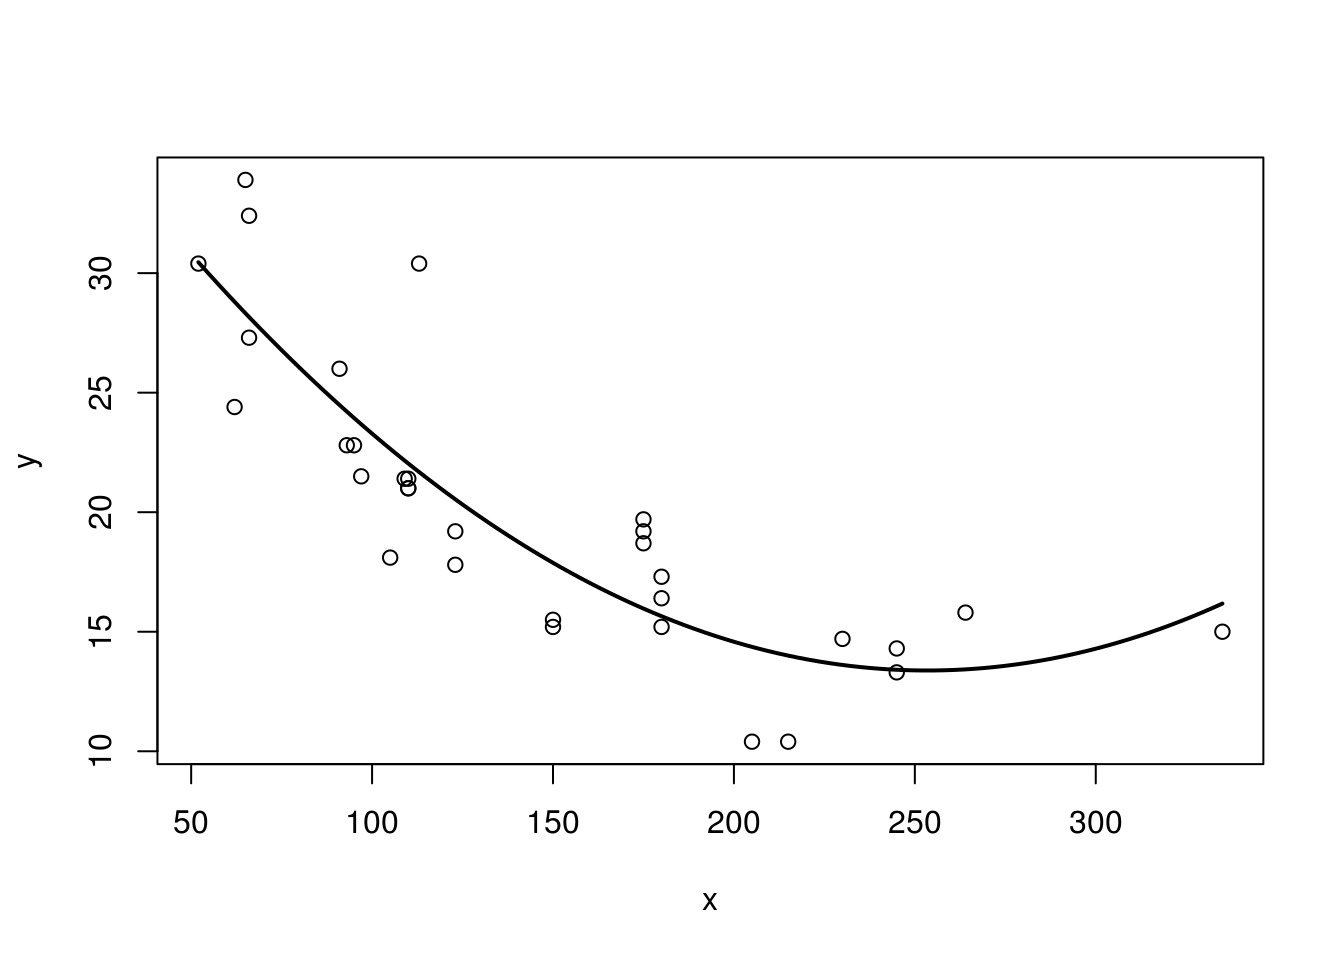
\includegraphics{ScPoEconometrics_files/figure-latex/non-line-cars-ols2-1} 

}

\caption{Better line with non-linear data!}\label{fig:non-line-cars-ols2}
\end{figure}

\section{\texorpdfstring{Analysing
\(Var(y)\)}{Analysing Var(y)}}\label{analysing-vary}

Analysis of Variance (ANOVA) refers to a method to decompose variation
in one variable as a function of several others. We can use this idea on
our outcome \(y\). Suppose we wanted to know the variance of \(y\),
keeping in mind that, by definition, \(y_i = \hat{y}_i + e_i\). We would
write

\begin{align}
Var(y) &= Var(\hat{y} + e)\\
 &= Var(\hat{y}) + Var(e) + 2 Cov(\hat{y},e)\\
 &= Var(\hat{y}) + Var(e) \label{eq:anova}
\end{align}

We have seen above in \ref{pred-resids} that the covariance between
prediction \(\hat{y}\) and error \(e\) is zero, that's why we have
\(Cov(\hat{y},e)=0\) in \eqref{eq:anova}. What this tells us in words is
that we can decompose the variance in the observed outcome \(y\) into a
part that relates to variance as \emph{explained by the model} and a
part that comes from unexplained variation. Finally, we know the
definition of \emph{variance}, and can thus write down the respective
formulae for each part:

\begin{itemize}
\tightlist
\item
  \(Var(y) = \frac{1}{N}\sum_{i=1}^N (y_i - \bar{y})^2\)
\item
  \(Var(\hat{y}) = \frac{1}{N}\sum_{i=1}^N (\hat{y_i} - \bar{y})^2\),
  because the mean of \(\hat{y}\) is \(\bar{y}\) as we know. Finally,
\item
  \(Var(e) = \frac{1}{N}\sum_{i=1}^N e_i^2\), because the mean of \(e\)
  is zero.
\end{itemize}

We can thus formulate how the total variation in outcome \(y\) is
aportioned between model and unexplained variation:

\begin{tip}
The total variation in outcome \(y\) (often called SST, or \emph{total
sum of squares}) is equal to the sum of explained squares (SSE) plus the
sum of residuals (SSR). We have thus \textbf{SST = SSE + SSR}.
\end{tip}

\section{\texorpdfstring{Assessing the \emph{Goodness of
Fit}}{Assessing the Goodness of Fit}}\label{assessing-the-goodness-of-fit}

In our setup, there exists a convenient measure for how good a
particular statistical model fits the data. It is called \(R^2\)
(\emph{R squared}), also called the \emph{coefficient of determination}.
We make use of the just introduced decomposition of variance, and write
the formula as

\begin{equation}
R^2 = \frac{\text{variance explained}}{\text{total variance}} = \frac{SSE}{SST} = 1 - \frac{SSR}{SST}\in[0,1]  \label{eq:Rsquared}
\end{equation}

It is easy to see that a \emph{good fit} is one where the sum of
\emph{explained} squares (SSE) is large relativ to the total variation
(SST). In such a case, we observe an \(R^2\) close to one. In the
opposite case, we will see an \(R^2\) close to zero. Notice that a small
\(R^2\) does not imply that the model is useless, just that it explains
a small fraction of the observed variation.

\section{An Example: A Log Wage
Equation}\label{an-example-a-log-wage-equation}

Let's consider the following example concerning wage data collected in
the 1976 Current Population Survey in the USA.\footnote{This example is
  close to the vignette of the
  \href{https://cloud.r-project.org/web/packages/wooldridge/index.html}{wooldridge}
  package, whose author I hereby thank for the excellent work.} We want
to investigate the relationship between average hourly earnings, and
years of education. Let's start with a plot:

\begin{Shaded}
\begin{Highlighting}[]
\KeywordTok{data}\NormalTok{(}\StringTok{"wage1"}\NormalTok{, }\DataTypeTok{package =} \StringTok{"wooldridge"}\NormalTok{)   }\CommentTok{# load data}

\CommentTok{# a function that returns a plot}
\NormalTok{plotfun <-}\StringTok{ }\ControlFlowTok{function}\NormalTok{(wage1,}\DataTypeTok{log=}\OtherTok{FALSE}\NormalTok{,}\DataTypeTok{rug =} \OtherTok{TRUE}\NormalTok{)\{}
\NormalTok{    y =}\StringTok{ }\NormalTok{wage1}\OperatorTok{$}\NormalTok{wage}
    \ControlFlowTok{if}\NormalTok{ (log)\{}
\NormalTok{        y =}\StringTok{ }\KeywordTok{log}\NormalTok{(wage1}\OperatorTok{$}\NormalTok{wage)}
\NormalTok{    \}}
    \KeywordTok{plot}\NormalTok{(}\DataTypeTok{y =}\NormalTok{ y,}
       \DataTypeTok{x =}\NormalTok{ wage1}\OperatorTok{$}\NormalTok{educ, }
       \DataTypeTok{col =} \StringTok{"red"}\NormalTok{, }\DataTypeTok{pch =} \DecValTok{21}\NormalTok{, }\DataTypeTok{bg =} \StringTok{"grey"}\NormalTok{,     }
       \DataTypeTok{cex=}\FloatTok{1.25}\NormalTok{, }\DataTypeTok{xaxt=}\StringTok{"n"}\NormalTok{, }\DataTypeTok{frame =} \OtherTok{FALSE}\NormalTok{,      }\CommentTok{# set default x-axis to none}
       \DataTypeTok{main =} \KeywordTok{ifelse}\NormalTok{(log,}\StringTok{"log(Wages) vs. Education, 1976"}\NormalTok{,}\StringTok{"Wages vs. Education, 1976"}\NormalTok{),}
       \DataTypeTok{xlab =} \StringTok{"years of education"}\NormalTok{, }
       \DataTypeTok{ylab =} \KeywordTok{ifelse}\NormalTok{(log,}\StringTok{"Log Hourly wages"}\NormalTok{,}\StringTok{"Hourly wages"}\NormalTok{))}
    \KeywordTok{axis}\NormalTok{(}\DataTypeTok{side =} \DecValTok{1}\NormalTok{, }\DataTypeTok{at =} \KeywordTok{c}\NormalTok{(}\DecValTok{0}\NormalTok{,}\DecValTok{6}\NormalTok{,}\DecValTok{12}\NormalTok{,}\DecValTok{18}\NormalTok{))         }\CommentTok{# add custom ticks to x axis}
    \ControlFlowTok{if}\NormalTok{ (rug) }\KeywordTok{rug}\NormalTok{(wage1}\OperatorTok{$}\NormalTok{wage, }\DataTypeTok{side=}\DecValTok{2}\NormalTok{, }\DataTypeTok{col=}\StringTok{"red"}\NormalTok{)        }\CommentTok{# add `rug` to y axis}
\NormalTok{\}}

\KeywordTok{par}\NormalTok{(}\DataTypeTok{mfcol =} \KeywordTok{c}\NormalTok{(}\DecValTok{2}\NormalTok{,}\DecValTok{1}\NormalTok{))  }\CommentTok{# set up a plot with 2 panels}
\CommentTok{# plot 1: standard scatter plot}
\KeywordTok{plotfun}\NormalTok{(wage1)}

\CommentTok{# plot 2: add a panel with histogram+density}
\KeywordTok{hist}\NormalTok{(wage1}\OperatorTok{$}\NormalTok{wage,}\DataTypeTok{prob =} \OtherTok{TRUE}\NormalTok{, }\DataTypeTok{col =} \StringTok{"grey"}\NormalTok{, }\DataTypeTok{border =} \StringTok{"red"}\NormalTok{, }
     \DataTypeTok{main =} \StringTok{"Histogram of wages and Density"}\NormalTok{,}\DataTypeTok{xlab =} \StringTok{"hourly wage"}\NormalTok{)}
\KeywordTok{lines}\NormalTok{(}\KeywordTok{density}\NormalTok{(wage1}\OperatorTok{$}\NormalTok{wage), }\DataTypeTok{col =} \StringTok{"black"}\NormalTok{, }\DataTypeTok{lw =} \DecValTok{2}\NormalTok{)}
\end{Highlighting}
\end{Shaded}

\begin{figure}

{\centering 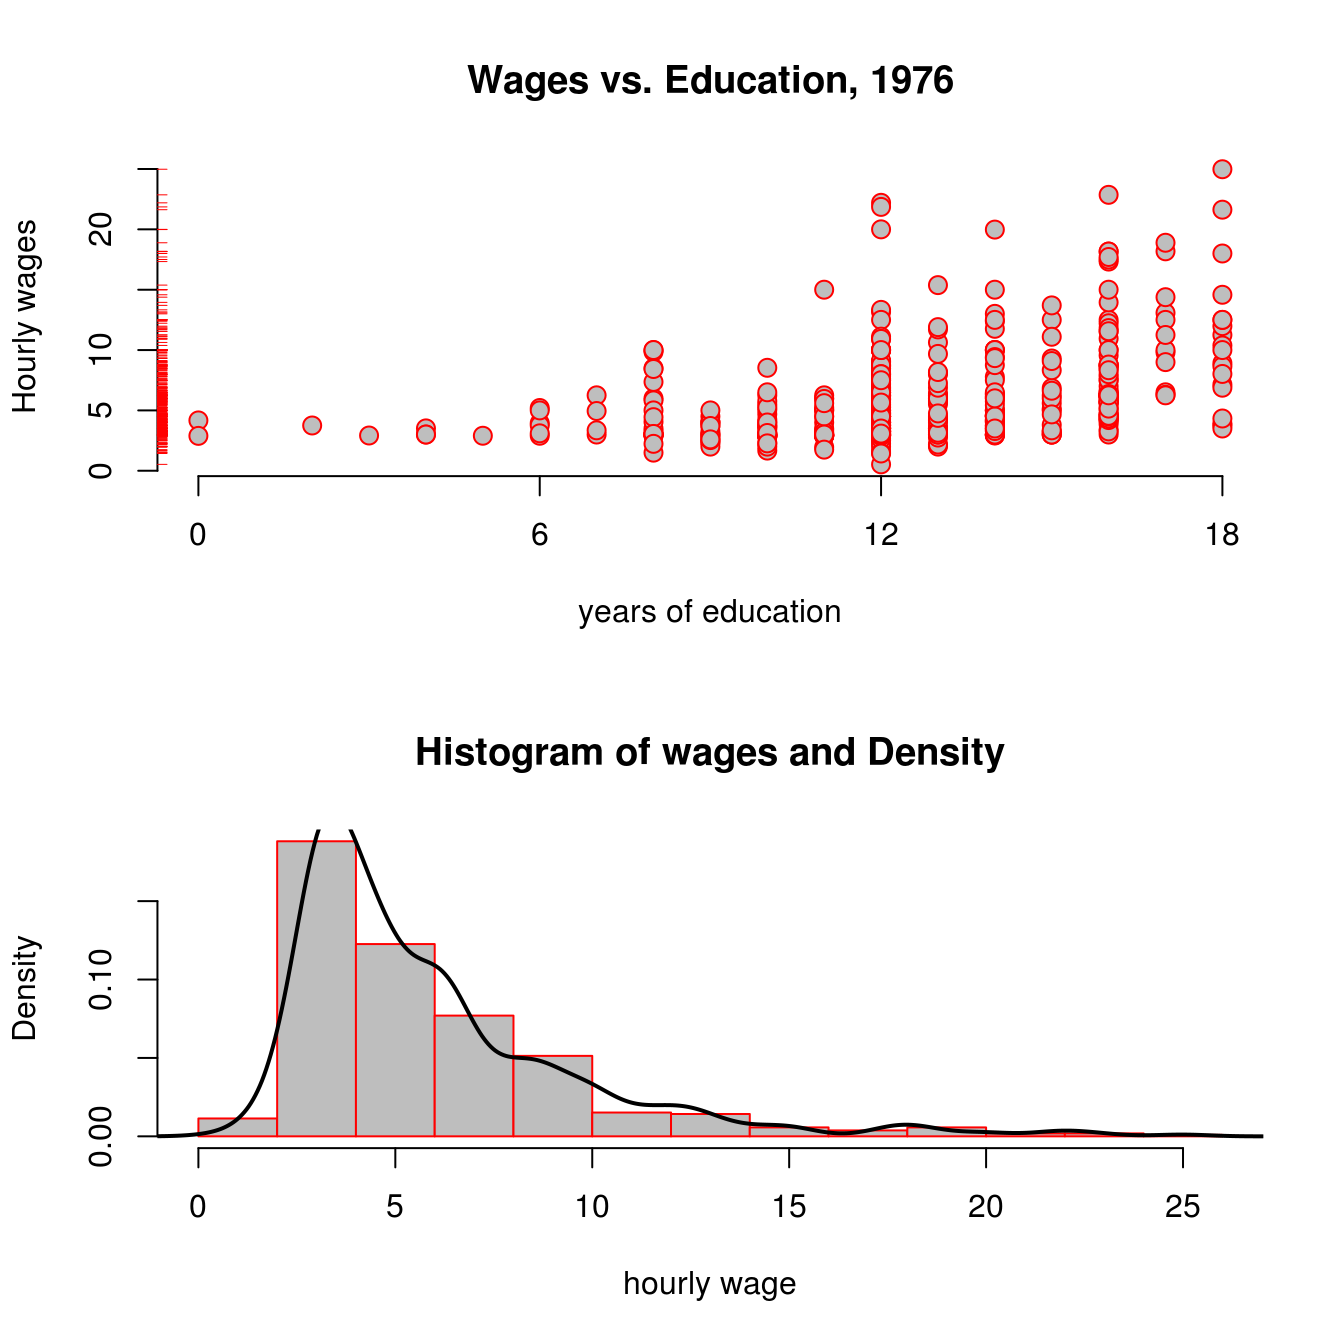
\includegraphics{ScPoEconometrics_files/figure-latex/wooldridge-wages-1} 

}

\caption{Wages vs Education from the wooldridge dataset wage1.}\label{fig:wooldridge-wages}
\end{figure}

Looking at the top panel of figure \ref{fig:wooldridge-wages}, you
notice two things: From the red ticks on the y axis, you see that wages
are very concentrated at around 5 USD per hour, with fewer and fewer
observations at higher rates; and second, that it seems that the hourly
wage seems to increase with higher education levels. The bottom panel
reinforces the first point, showing that the estimated pdf (probability
density function) shown as a black line has a very long right tail:
there are always fewer and fewer, but always larger and larger values of
hourly wage in the data.

\begin{warning}
You have seen this shape of a distribution in the tutorial for chapter 2
already! Do you remember the name of this particular shape of a
distribution? (why not type
\texttt{ScPoEconometrics::runTutorial(\textquotesingle{}chapter2\textquotesingle{})})
to check?
\end{warning}

Let's run a first regression on this data to generate some intution:

\begin{equation}
\text{wage}_i = b_0 + b_1 \text{educ}_i + e_i \label{eq:wage}
\end{equation}

We use the \texttt{lm} function for this purpose as follows:

\begin{Shaded}
\begin{Highlighting}[]
\NormalTok{hourly_wage <-}\StringTok{ }\KeywordTok{lm}\NormalTok{(}\DataTypeTok{formula =}\NormalTok{ wage }\OperatorTok{~}\StringTok{ }\NormalTok{educ, }\DataTypeTok{data =}\NormalTok{ wage1)}
\end{Highlighting}
\end{Shaded}

and we can add the resulting regression line to our above plot:

\begin{Shaded}
\begin{Highlighting}[]
\KeywordTok{plotfun}\NormalTok{(wage1)}
\KeywordTok{abline}\NormalTok{(hourly_wage, }\DataTypeTok{col =} \StringTok{'black'}\NormalTok{, }\DataTypeTok{lw =} \DecValTok{2}\NormalTok{) }\CommentTok{# add regression line}
\end{Highlighting}
\end{Shaded}

\begin{figure}

{\centering 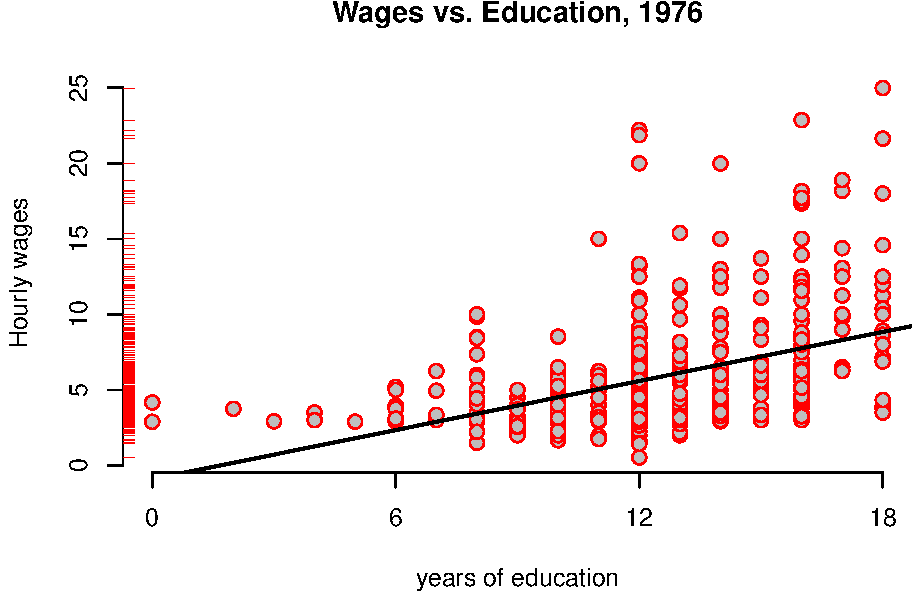
\includegraphics{ScPoEconometrics_files/figure-latex/wooldridge-wages2-1} 

}

\caption{Wages vs Education from the wooldridge dataset wage1, with regression}\label{fig:wooldridge-wages2}
\end{figure}

The \texttt{hourly\_wage} object contains the results of this
estimation. We can get a summary of those results with the
\texttt{summary} method:

\begin{Shaded}
\begin{Highlighting}[]
\KeywordTok{summary}\NormalTok{(hourly_wage)}
\end{Highlighting}
\end{Shaded}

\begin{verbatim}
#OUT> 
#OUT> Call:
#OUT> lm(formula = wage ~ educ, data = wage1)
#OUT> 
#OUT> Residuals:
#OUT>     Min      1Q  Median      3Q     Max 
#OUT> -5.3396 -2.1501 -0.9674  1.1921 16.6085 
#OUT> 
#OUT> Coefficients:
#OUT>             Estimate Std. Error t value Pr(>|t|)    
#OUT> (Intercept) -0.90485    0.68497  -1.321    0.187    
#OUT> educ         0.54136    0.05325  10.167   <2e-16 ***
#OUT> ---
#OUT> Signif. codes:  0 '***' 0.001 '**' 0.01 '*' 0.05 '.' 0.1 ' ' 1
#OUT> 
#OUT> Residual standard error: 3.378 on 524 degrees of freedom
#OUT> Multiple R-squared:  0.1648,  Adjusted R-squared:  0.1632 
#OUT> F-statistic: 103.4 on 1 and 524 DF,  p-value: < 2.2e-16
\end{verbatim}

The main interpretation of this table can be read off the column
labelled \emph{Estimate}, reporting estimated coefficients \(b_0,b_1\):

\begin{enumerate}
\def\labelenumi{\arabic{enumi}.}
\tightlist
\item
  With zero year of education, the hourly wage is about -0.9 dollars per
  hour (row named \texttt{(Intercept)})
\item
  Each additional year of education increase hourly wage by 54 cents.
  (row named \texttt{educ})
\item
  For example, for 15 years of education, we predict roughly -0.9 +
  0.541 * 15 = 7.215 dollars/h.
\end{enumerate}

\section{Scaling Regressions}\label{scaling-regressions}

\begin{tip}
Regression estimates (\(b_0, b_1\)) are in the scale \emph{of the data}.
The actual \emph{value} of the estimates will vary, if we change the
scale of the data. The overall fit of the model to the data would
\emph{not} change, however, so that the \(R^2\) statistic would be
constant.
\end{tip}

Suppose we wanted to use the above estimates to report the effect of
years of education on \emph{annual} wages instead of \emph{hourly} ones.
Let's assume we have full-time workers, 7h per day, 5 days per week, 45
weeks per year. Calling this factor
\(\delta = 7 \times 5 \times 45 = 1575\), we have that \(x\) dollars per
hour imply \(x \times \delta = x \times 1575\) dollars per year.

What would be the effect of using \(\tilde{y} = wage \times 1575\)
instead of \(y = wage\) as outcome variable on our regression
coefficients \(b_0\) and \(b_1\)? Well, let's try!

\% Table created by stargazer v.5.2.2 by Marek Hlavac, Harvard
University. E-mail: hlavac at fas.harvard.edu \% Date and time: Mon, Nov
25, 2019 - 10:11:16 PM

\begin{table}[!htbp] \centering 
  \caption{Effect of Scaling on Coefficients} 
  \label{} 
\begin{tabular}{@{\extracolsep{5pt}}lcc} 
\\[-1.8ex]\hline 
\hline \\[-1.8ex] 
 & \multicolumn{2}{c}{\textit{Dependent variable:}} \\ 
\cline{2-3} 
\\[-1.8ex] & wage & annual\_wage \\ 
\\[-1.8ex] & (1) & (2)\\ 
\hline \\[-1.8ex] 
 educ & 0.541$^{***}$ & 852.641$^{***}$ \\ 
  & (0.053) & (83.866) \\ 
  & & \\ 
 Constant & $-$0.905 & $-$1,425.141 \\ 
  & (0.685) & (1,078.824) \\ 
  & & \\ 
\hline \\[-1.8ex] 
Observations & 526 & 526 \\ 
R$^{2}$ & 0.165 & 0.165 \\ 
Adjusted R$^{2}$ & 0.163 & 0.163 \\ 
Residual Std. Error (df = 524) & 3.378 & 5,320.963 \\ 
F Statistic (df = 1; 524) & 103.363$^{***}$ & 103.363$^{***}$ \\ 
\hline 
\hline \\[-1.8ex] 
\textit{Note:}  & \multicolumn{2}{r}{$^{*}$p$<$0.1; $^{**}$p$<$0.05; $^{***}$p$<$0.01} \\ 
\end{tabular} 
\end{table}

Let's call the coefficients in the column labelled (1) as \(b_0\) and
\(b_1\), and let's call the ones in column (2) \(b_0^*\) and \(b_1^*\).
In column (1) we see that another year increaeses hourly wage by 0.54
dollars, as before. In column (2), the corresponding number is 852.64,
i.e.~another year of education will increase \emph{annual} wages by
852.64 dollars, on average. Notice however, that
\(b_0 \times \delta = -0.9 \times 1575 = -1425.14 = b_0^*\) and that
\(b_1 \times \delta = 0.54 \times 1575 = 852.64 = b_1^*\), that is we
just had to multiply both coefficients by the scaling factor applied to
original outcome \(y\) to obtain our new coefficients \(b_0^*\) and
\(b_1^*\)! Also, observe that the \(R^2\)s of both regressions are
identical! So, really, we did not have to run the regression in column
(2) at all to make this change: multiplying all coefficients through by
\(\delta\) is enough in this case. We keep the identically same fit to
the data.

Rescaling the regressors \(x\) is slightly different, but it's easy to
work out \emph{how} different, given the linear nature of the covariance
operator, which is part of the OLS estimator. Suppose we rescale \(x\)
by the number \(c\). Then, using the OLS formula in \eqref{eq:beta1hat},
we see that we get new slope coefficient \(b_1^*\) via

\begin{align} 
b_1^* &= \frac{Cov(cx,y)}{Var(cx)} \\ 
      &= \frac{cCov(x,y)}{c^2 Var(x)} \\
      &= \frac{1}{c} b_1.
\end{align}

As for the intercept, and by using \eqref{eq:beta0hat}

\begin{align} 
b_0^* &= \bar{y} -             b_1^* \frac{1}{N}\sum_{i=1}^N c \cdot x_i \\ 
      &= \bar{y} -             b_1^* \frac{c}{N}\sum_{i=1}^N x_i  \\
      &= \bar{y} - \frac{1}{c} b_1 c * \bar{x}  \\
      &= \bar{y} -  b_1 * \bar{x}  \\
      &= b_0
\end{align}

That is, we change the slope by the \emph{inverse} of the scaling factor
applied to regressor \(x\), but the intercept is unaffected from this.
You should play around for a while with our rescaling app to get a
feeling for this:

\begin{Shaded}
\begin{Highlighting}[]
\KeywordTok{library}\NormalTok{(ScPoEconometrics)}
\KeywordTok{launchApp}\NormalTok{(}\StringTok{'Rescale'}\NormalTok{)}
\end{Highlighting}
\end{Shaded}

\section{\texorpdfstring{A Particular Rescaling: The \(\log\)
Transform}{A Particular Rescaling: The \textbackslash{}log Transform}}\label{a-particular-rescaling-the-log-transform}

The natural logarithm is a particularly important transformation that we
often encounter in economics. Why would we transform a variable with the
\(\log\) function to start with?

\begin{enumerate}
\def\labelenumi{\arabic{enumi}.}
\tightlist
\item
  Several important economic variables (like wages, city size, firm
  size, etc) are approximately \emph{log-normally} distributed. By
  transforming them with the \(\log\), we obtain an approximately
  \emph{normally} distributed variable, which has desirable properties
  for our regression.
\item
  Applying the \(\log\) reduces the impact of outliers.
\item
  The transformation allows for a convenient interpretation in terms of
  \emph{percentage changes} of the outcome variable.
\end{enumerate}

Let's investigate this issue in our running example by transforming the
wage data above. Look back at the bottom panel of figure
\ref{fig:wooldridge-wages}: Of course you saw immediately that this
looked a lot like a log-normal distribution, so point 1. above applies.
We modify the left hand side of equation \eqref{eq:wage}:

\begin{equation}
\log(\text{wage}_i) = b_0 + b_1 \text{educ}_i + e_i \label{eq:log-wage}
\end{equation}

Let's use the \texttt{update} function to modify our previous regression
model:

\begin{Shaded}
\begin{Highlighting}[]
\NormalTok{log_hourly_wage =}\StringTok{ }\KeywordTok{update}\NormalTok{(hourly_wage, }\KeywordTok{log}\NormalTok{(wage) }\OperatorTok{~}\StringTok{ }\NormalTok{., }\DataTypeTok{data =}\NormalTok{ wage1)}
\end{Highlighting}
\end{Shaded}

The \texttt{update} function takes an existing \texttt{lm} object, like
\texttt{hourly\_wage} here, and updates the \texttt{formula}. Here the
\texttt{.} on the right hand side means \emph{leave unchanged} (so the
RHS stays unchanged). How do our pictures change?

\begin{Shaded}
\begin{Highlighting}[]
\KeywordTok{par}\NormalTok{(}\DataTypeTok{mfrow =} \KeywordTok{c}\NormalTok{(}\DecValTok{1}\NormalTok{,}\DecValTok{2}\NormalTok{))}

\KeywordTok{plotfun}\NormalTok{(wage1,}\DataTypeTok{rug =} \OtherTok{FALSE}\NormalTok{)}
\KeywordTok{abline}\NormalTok{(hourly_wage, }\DataTypeTok{col =} \StringTok{'black'}\NormalTok{, }\DataTypeTok{lw =} \DecValTok{2}\NormalTok{) }\CommentTok{# add regression line}

\KeywordTok{plotfun}\NormalTok{(wage1,}\DataTypeTok{log =} \OtherTok{TRUE}\NormalTok{, }\DataTypeTok{rug =} \OtherTok{FALSE}\NormalTok{)}
\KeywordTok{abline}\NormalTok{(log_hourly_wage, }\DataTypeTok{col =} \StringTok{'black'}\NormalTok{, }\DataTypeTok{lw =} \DecValTok{2}\NormalTok{) }\CommentTok{# add regression line}
\end{Highlighting}
\end{Shaded}

\begin{center}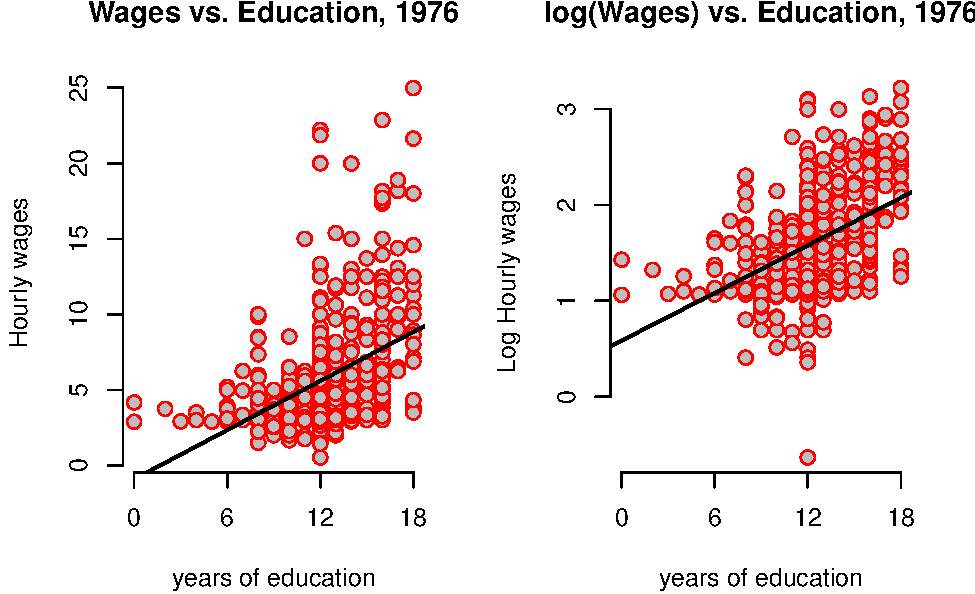
\includegraphics{ScPoEconometrics_files/figure-latex/logplot-1} \end{center}

\begin{Shaded}
\begin{Highlighting}[]
\KeywordTok{par}\NormalTok{(}\DataTypeTok{mfrow =} \KeywordTok{c}\NormalTok{(}\DecValTok{1}\NormalTok{,}\DecValTok{1}\NormalTok{))}
\end{Highlighting}
\end{Shaded}

It \emph{looks as if} the regression line has the same slope, but beware
of the different scales of the y-axis! You can clearly see that all
y-values have been compressed by the log transformation. The log case
behaves differently from our \emph{scaling by a constant number} case
above because it is a \emph{nonlinear} function. Let's compare the
output between both models:

\% Table created by stargazer v.5.2.2 by Marek Hlavac, Harvard
University. E-mail: hlavac at fas.harvard.edu \% Date and time: Mon, Nov
25, 2019 - 10:11:17 PM

\begin{table}[!htbp] \centering 
  \caption{Log Transformed Equation} 
  \label{} 
\begin{tabular}{@{\extracolsep{5pt}}lcc} 
\\[-1.8ex]\hline 
\hline \\[-1.8ex] 
 & \multicolumn{2}{c}{\textit{Dependent variable:}} \\ 
\cline{2-3} 
\\[-1.8ex] & wage & log(wage) \\ 
\\[-1.8ex] & (1) & (2)\\ 
\hline \\[-1.8ex] 
 educ & 0.541$^{***}$ & 0.083$^{***}$ \\ 
  & (0.053) & (0.008) \\ 
  & & \\ 
 Constant & $-$0.905 & 0.584$^{***}$ \\ 
  & (0.685) & (0.097) \\ 
  & & \\ 
\hline \\[-1.8ex] 
Observations & 526 & 526 \\ 
R$^{2}$ & 0.165 & 0.186 \\ 
Adjusted R$^{2}$ & 0.163 & 0.184 \\ 
Residual Std. Error (df = 524) & 3.378 & 0.480 \\ 
F Statistic (df = 1; 524) & 103.363$^{***}$ & 119.582$^{***}$ \\ 
\hline 
\hline \\[-1.8ex] 
\textit{Note:}  & \multicolumn{2}{r}{$^{*}$p$<$0.1; $^{**}$p$<$0.05; $^{***}$p$<$0.01} \\ 
\end{tabular} 
\end{table}

The interpretation of the transformed model in column (2) is now the
following:

\begin{note}
We call a regression of the form \(\log(y) = b_0 + b_1 x + u\) a
\emph{log-level} specification, because we regressed the log of a
variable on the level (i.e not the log!) of another variable. Here, the
impact of increasing \(x\) by one unit is to increase \(y\) by
\(100 \times b_1\) \textbf{percent}. In our example: an additional year
of education will increase hourly wages by 8.3\%. Notice that this is
very different from saying \emph{\ldots{}increases log hourly wages by
8.3\%}, which is wrong.
\end{note}

Notice that the \(R^2\) slightly improved, so have a better fit to the
data. This is due the fact that the log compressed large outlier values.
Whether we apply the \(log\) to left or right-hand side variables makes
a difference, as outlined in this important table:

\label{tab:loglog} Common Regression Specifications

\begin{longtable}[]{@{}ccccc@{}}
\toprule
Specification & Outcome Var & Regressor & Interpretation of \(b_1\) &
Comment\tabularnewline
\midrule
\endhead
Level-level & y & x & \(\Delta y = b_1 \Delta x\) &
Standard\tabularnewline
Level-log & y & \(\log(x)\) & \(\Delta y = \frac{b_1}{100} \Delta x\) &
less frequent\tabularnewline
Log-level & \(\log(y)\) & x & \(\% \Delta y = (100 b_1) \Delta\) x &
Semi-elasticity\tabularnewline
Log-Log & \(\log(y)\) & \(\log(x)\) & \(\% \Delta y = \% \Delta\) b\_1 x
& Elasticity\tabularnewline
\bottomrule
\end{longtable}

You may remember from your introductory micro course what the definition
of the \emph{elasticity} of \(y\) with respect to \(x\) is: This number
tells us by how many percent \(y\) will change, if we change \(x\) by
one percent. Let's look at another example from the \texttt{wooldridge}
package of datasets, this time concerning CEO salaries and their
relationship with company sales.

\begin{Shaded}
\begin{Highlighting}[]
\KeywordTok{data}\NormalTok{(}\StringTok{"ceosal1"}\NormalTok{, }\DataTypeTok{package =} \StringTok{"wooldridge"}\NormalTok{)  }
\KeywordTok{par}\NormalTok{(}\DataTypeTok{mfrow =} \KeywordTok{c}\NormalTok{(}\DecValTok{1}\NormalTok{,}\DecValTok{2}\NormalTok{))}
\KeywordTok{plot}\NormalTok{(salary }\OperatorTok{~}\StringTok{ }\NormalTok{sales, }\DataTypeTok{data =}\NormalTok{ ceosal1, }\DataTypeTok{main =} \StringTok{"Sales vs Salaries"}\NormalTok{,}\DataTypeTok{xaxt =} \StringTok{"n"}\NormalTok{,}\DataTypeTok{frame =} \OtherTok{FALSE}\NormalTok{)}
\KeywordTok{axis}\NormalTok{(}\DecValTok{1}\NormalTok{, }\DataTypeTok{at =} \KeywordTok{c}\NormalTok{(}\DecValTok{0}\NormalTok{,}\DecValTok{40000}\NormalTok{, }\DecValTok{80000}\NormalTok{))}
\KeywordTok{rug}\NormalTok{(ceosal1}\OperatorTok{$}\NormalTok{salary,}\DataTypeTok{side =} \DecValTok{2}\NormalTok{)}
\KeywordTok{rug}\NormalTok{(ceosal1}\OperatorTok{$}\NormalTok{sales,}\DataTypeTok{side =} \DecValTok{1}\NormalTok{)}
\KeywordTok{plot}\NormalTok{(}\KeywordTok{log}\NormalTok{(salary) }\OperatorTok{~}\StringTok{ }\KeywordTok{log}\NormalTok{(sales), }\DataTypeTok{data =}\NormalTok{ ceosal1, }\DataTypeTok{main =} \StringTok{"Log(Sales) vs Log(Salaries)"}\NormalTok{)}
\end{Highlighting}
\end{Shaded}

\begin{figure}

{\centering 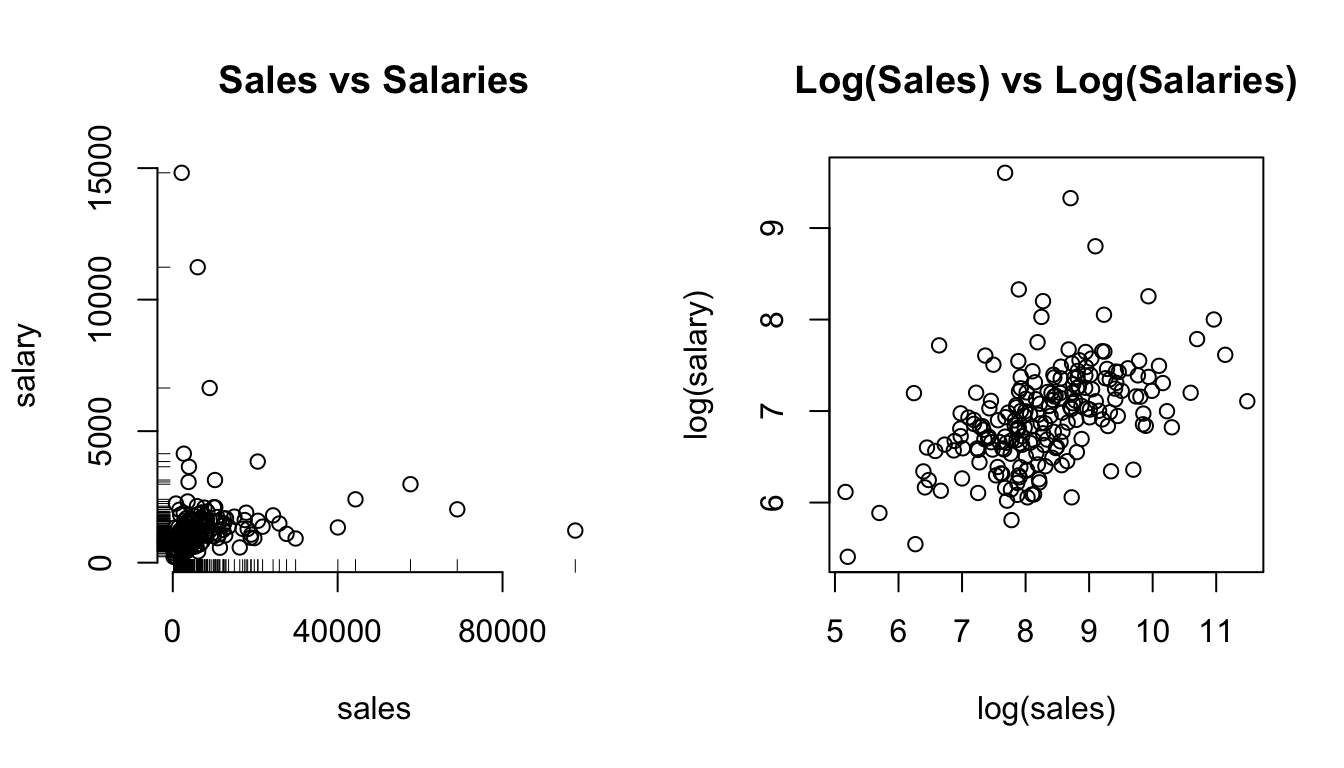
\includegraphics{ScPoEconometrics_files/figure-latex/ceo-sal-1} 

}

\caption{The effect of log-transforming highly skewed data.}\label{fig:ceo-sal}
\end{figure}

In the left panel of figure \ref{fig:ceo-sal} you clearly see that both
\texttt{sales} and \texttt{salary} have very long right tails, as
indicated by the rug plots on either axis. As a consequence, the points
are clustered in the bottom left corner of the plot. We suspect a
positive relationship, but it's hard to see. Contrast this with the
right panel, where both axis have been log transformed: the points are
nicely spread out, clearly spelling out a positive correlation. Let's
see what this gives in a regression model!

\[
\text{logsalary} = 4.82 + 0.26(\text{logsales}) + \epsilon
\]

Refering back at table \ref{tab:loglog}, here we have a log-log
specification. Therefore we interpret this regression as follows:

\begin{tip}
In a log-log equation, the slope coefficient \(b_1\) is the
\emph{elasticity of \(y\) with respect to changes in \(x\)}. Here: A 1\%
increase in sales is associated to a 0.26\% increase in CEO salaries.
Note, again, that there is no \emph{log} in this statement.
\end{tip}

\chapter{Multiple Regression}\label{multiple-reg}

We can extend the discussion from chapter \ref{linreg} to more than one
explanatory variable. For example, suppose that instead of only \(x\) we
now had \(x_1\) and \(x_2\) in order to explain \(y\). Everything we've
learned for the single variable case applies here as well. Instead of a
regression \emph{line}, we now get a regression \emph{plane}, i.e.~an
object representable in 3 dimenions: \((x_1,x_2,y)\). As an example,
suppose we wanted to explain how many \emph{miles per gallon}
(\texttt{mpg}) a car can travel as a function of its \emph{horse power}
(\texttt{hp}) and its \emph{weight} (\texttt{wt}). In other words we
want to estimate the equation

\begin{equation}
mpg_i = b_0 + b_1 hp_i + b_2 wt_i + e_i \label{eq:abline2d}
\end{equation}

on our built-in dataset of cars (\texttt{mtcars}):

\begin{Shaded}
\begin{Highlighting}[]
\KeywordTok{head}\NormalTok{(}\KeywordTok{subset}\NormalTok{(mtcars, }\DataTypeTok{select =} \KeywordTok{c}\NormalTok{(mpg,hp,wt)))}
\end{Highlighting}
\end{Shaded}

\begin{verbatim}
#OUT>                    mpg  hp    wt
#OUT> Mazda RX4         21.0 110 2.620
#OUT> Mazda RX4 Wag     21.0 110 2.875
#OUT> Datsun 710        22.8  93 2.320
#OUT> Hornet 4 Drive    21.4 110 3.215
#OUT> Hornet Sportabout 18.7 175 3.440
#OUT> Valiant           18.1 105 3.460
\end{verbatim}

How do you think \texttt{hp} and \texttt{wt} will influence how many
miles per gallon of gasoline each of those cars can travel? In other
words, what do you expect the signs of \(b_1\) and \(b_2\) to be?

With two explanatory variables as here, it is still possible to
visualize the regression plane, so let's start with this as an answer.
The OLS regression plane through this dataset looks like in figure
\ref{fig:plane3D-reg}:

\begin{figure}

{\centering 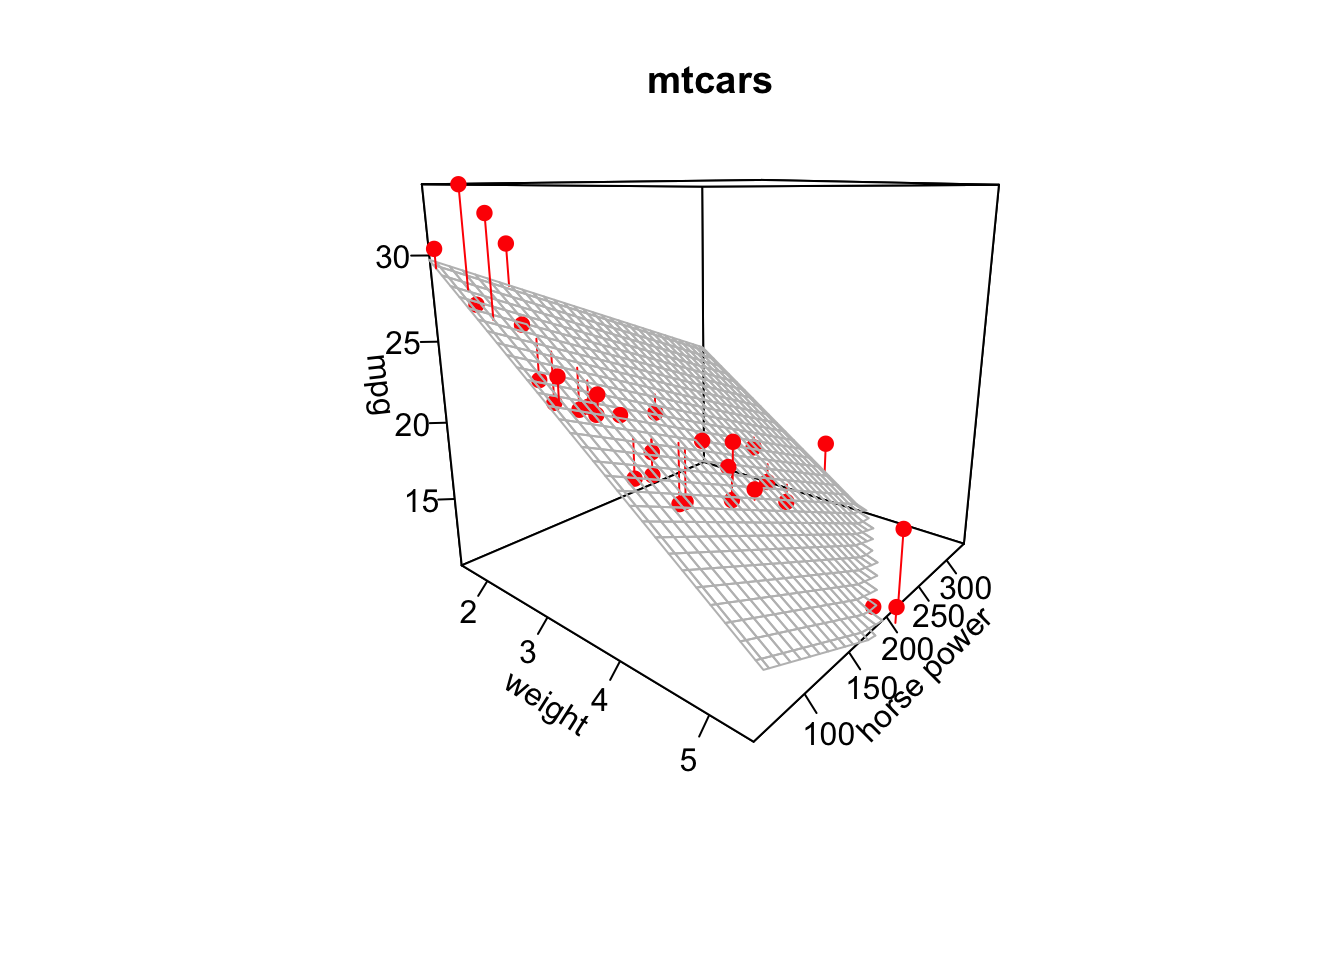
\includegraphics{ScPoEconometrics_files/figure-latex/plane3D-reg-1} 

}

\caption{Multiple Regression - a plane in 3D. The red lines indicate the residual for each observation.}\label{fig:plane3D-reg}
\end{figure}

This visualization shows a couple of things: the data are shown with red
points and the grey plane is the one resulting from OLS estimation of
equation \eqref{eq:abline2d}. You should realize that this is exactly the
same story as told in figure \ref{fig:line-arrows} - just in three
dimensions!

Furthermore, \emph{multiple} regression refers the fact that there could
be \emph{more} than two regressors. In fact, you could in principle have
\(K\) regressors, and our theory developed so far would still be valid:

\begin{align}
\hat{y}_i &= b_0 + b_1 x_{1i} +   b_2 x_{2i} + \dots + b_K x_{Ki}\\
e_i &= y_i - \hat{y}_i \label{eq:multiple-reg}
\end{align}

Just as before, the least squares method chooses numbers
\((b_0,b_1,\dots,b_K)\) to as to minimize SSR, exactly as in the
minimization problem for the one regressor case seen in
\eqref{eq:ols-min}.

\section{All Else Equal}\label{ceteris}

We can see from the above plot that cars with more horse power and
greater weight, in general travel fewer miles per gallon of combustible.
Hence, we observe a plane that is downward sloping in both the
\emph{weight} and \emph{horse power} directions. Suppose now we wanted
to know impact of \texttt{hp} on \texttt{mpg} \emph{in isolation}, so as
if we could ask

\begin{tip}
Keeping the value of \(wt\) fixed for a certain car, what would be the
impact on \(mpg\) be if we were to increase \textbf{only} its \(hp\)?
Put differently, keeping \textbf{all else equal}, what's the impact of
changing \(hp\) on \(mpg\)?
\end{tip}

 We ask this kind of question all the time in econometrics. In figure
\ref{fig:plane3D-reg} you clearly see that both explanatory variables
have a negative impact on the outcome of interest: as one increases
either the horse power or the weight of a car, one finds that miles per
gallon decreases. What is kind of hard to read off is \emph{how
negative} an impact each variable has in isolation.

As a matter of fact, the kind of question asked here is so common that
it has got its own name: we'd say ``\emph{ceteris paribus}, what is the
impact of \texttt{hp} on \texttt{mpg}?''. \emph{ceteris paribus} is
latin and means \emph{the others equal}, i.e.~all other variables fixed.
In terms of our model in \eqref{eq:abline2d}, we want to know the
following quantity:

\begin{equation}
\frac{\partial mpg_i}{\partial hp_i} = b_1 \label{eq:abline2d-deriv}
\end{equation}

The \(\partial\) sign denotes a \emph{partial derivative} of the
function describing \texttt{mpg} with respect to the variable
\texttt{hp}. It measures \emph{how the value of \texttt{mpg} changes, as
we change the value of \texttt{hp} ever so slightly}. In our context,
this means: \emph{keeping all other variables fixed, what is the effect
of \texttt{hp} on \texttt{mpg}?}. We call the value of coefficient
\(b_1\) therefore also the \emph{partial effect} of \texttt{hp} on
\texttt{mpg}. In terms of our dataset, we use \texttt{R} to run the
following \textbf{multiple regression}:

\begin{verbatim}
#OUT> 
#OUT> Call:
#OUT> lm(formula = mpg ~ wt + hp, data = mtcars)
#OUT> 
#OUT> Residuals:
#OUT>    Min     1Q Median     3Q    Max 
#OUT> -3.941 -1.600 -0.182  1.050  5.854 
#OUT> 
#OUT> Coefficients:
#OUT>             Estimate Std. Error t value Pr(>|t|)    
#OUT> (Intercept) 37.22727    1.59879  23.285  < 2e-16 ***
#OUT> wt          -3.87783    0.63273  -6.129 1.12e-06 ***
#OUT> hp          -0.03177    0.00903  -3.519  0.00145 ** 
#OUT> ---
#OUT> Signif. codes:  0 '***' 0.001 '**' 0.01 '*' 0.05 '.' 0.1 ' ' 1
#OUT> 
#OUT> Residual standard error: 2.593 on 29 degrees of freedom
#OUT> Multiple R-squared:  0.8268,  Adjusted R-squared:  0.8148 
#OUT> F-statistic: 69.21 on 2 and 29 DF,  p-value: 9.109e-12
\end{verbatim}

From this table you see that the coefficient on \texttt{wt} has value
-3.87783. You can interpret this as follows:

\begin{warning}
Holding all other variables fixed at their observed values - or
\emph{ceteris paribus} - a one unit increase in \(wt\) implies a
-3.87783 units change in \(mpg\). In other words, increasing the weight
of a car by 1000 pounds (lbs), will lead to 3.88 miles less travelled
per gallon. Similarly, a car with one additional horse power means that
we will travel 0.03177 fewer miles per gallon of gasoline, \emph{all
else (i.e. \(wt\)) equal}.
\end{warning}

\section{Multicolinearity}\label{multicol}

One important requirement for multiple regression is that the data be
\textbf{not linearly dependent}: Each variable should provide at least
some new information for the outcome, and it cannot be replicated as a
linear combination of other variables. Suppose that in the example
above, we had a variable \texttt{wtplus} defined as \texttt{wt\ +\ 1},
and we included this new variable together with \texttt{wt} in our
regression. In this case, \texttt{wtplus} provides no new information.
It's enough to know \(wt\), and add \(1\) to it. In this sense,
\texttt{wt\_plus} is a redundant variable and should not be included in
the model. Notice that this holds only for \emph{linearly} dependent
variables - \emph{nonlinear} transformations (like for example \(wt^2\))
are exempt from this rule. Here is why:

\begin{align}
y &= b_0 + b_1 \text{wt} + b_2 \text{wtplus} + e \\
  &= b_0 + b_1 \text{wt} + b_2 (\text{wt} + 1) + e \\
  &= (b_0 + b_2) + \text{wt} (b_1 + b_2) + e
\end{align}

This shows that we cannot \emph{identify} the regression coefficients in
case of linearly dependent data. Variation in the variable \texttt{wt}
identifies a different coefficient, say \(\gamma = b_1 + b_2\), from
what we actually wanted: separate estimates for \(b_1,b_2\).

\begin{note}
We cannot have variables which are \emph{linearly dependent}, or
\emph{perfectly colinear}. This is known as the \textbf{rank condition}.
In particular, the condition dictates that we need at least
\(N \geq K+1\), i.e.~more observations than coefficients. The greater
the degree of linear dependence amongst our explanatory variables, the
less information we can extract from them, and our estimates becomes
\emph{less precise}.
\end{note}

\section{Log Wage Equation}\label{log-wage-equation}

Let's go back to our previous example of the relationship between log
wages and education. How does this relationship change if we also think
that experience in the labor market has an impact, next to years of
education? Here is a picture:

\begin{figure}

{\centering 
\includegraphics{ScPoEconometrics_files/figure-latex/plane3D-lwage-1} 

}

\caption{Log wages vs education and experience in 3D.}\label{fig:plane3D-lwage}
\end{figure}

Let's add even more variables! For instance, what's the impact of
experience in the labor market, and time spent with the current
employer? Let's first look at how those variables co-vary with each
other:

\begin{Shaded}
\begin{Highlighting}[]
\NormalTok{cmat =}\StringTok{ }\KeywordTok{round}\NormalTok{(}\KeywordTok{cor}\NormalTok{(}\KeywordTok{subset}\NormalTok{(wage1,}\DataTypeTok{select =} \KeywordTok{c}\NormalTok{(lwage,educ,exper,tenure))),}\DecValTok{2}\NormalTok{) }\CommentTok{# correlation matrix}
\NormalTok{corrplot}\OperatorTok{::}\KeywordTok{corrplot}\NormalTok{(cmat,}\DataTypeTok{type =} \StringTok{"upper"}\NormalTok{,}\DataTypeTok{method =} \StringTok{"ellipse"}\NormalTok{)}
\end{Highlighting}
\end{Shaded}

\begin{figure}

{\centering 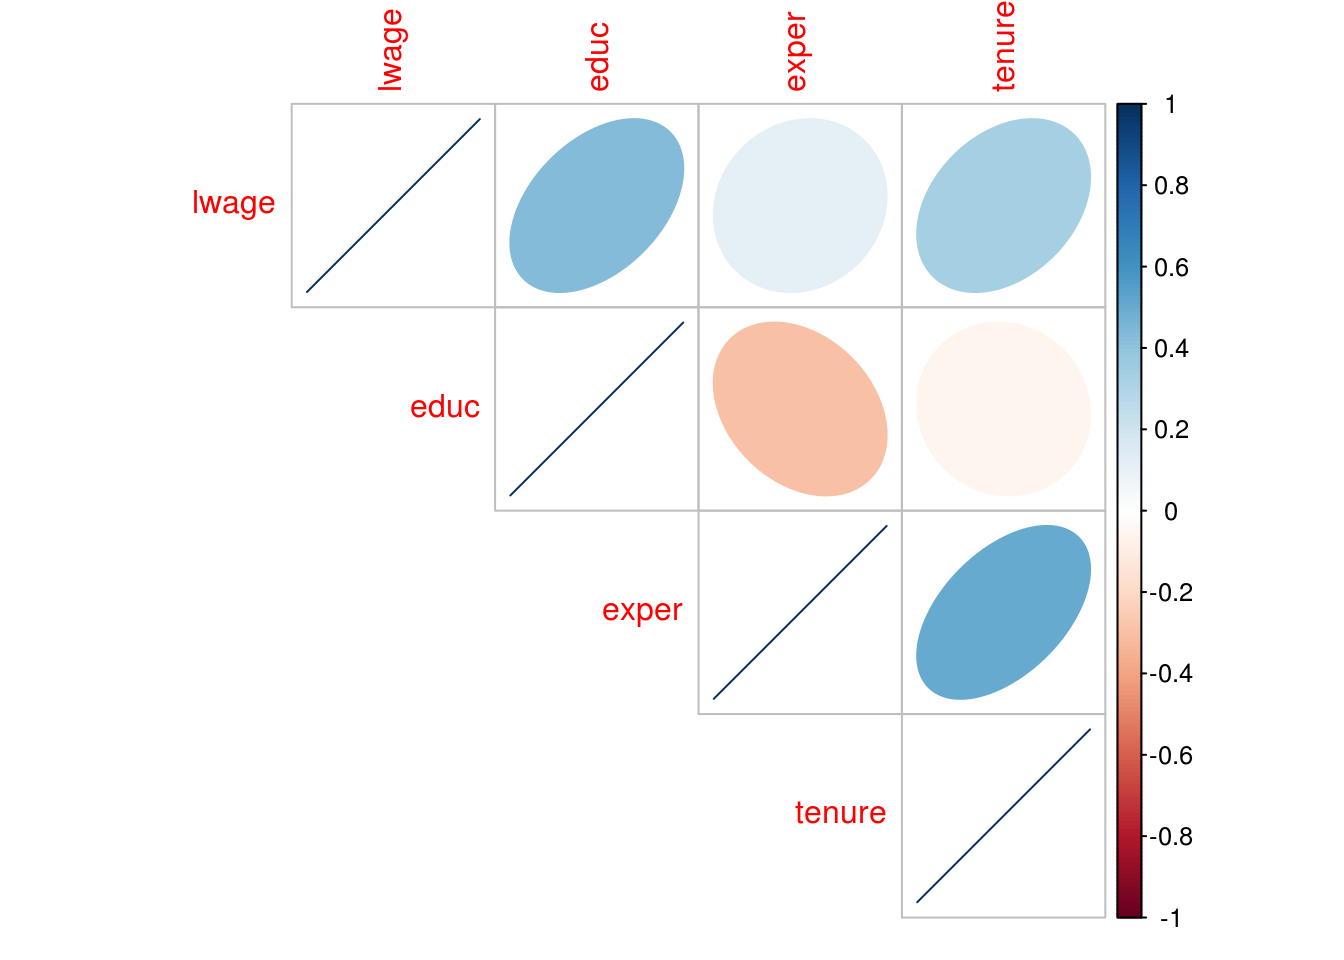
\includegraphics{ScPoEconometrics_files/figure-latex/corrplot-1} 

}

\caption{correlation plot}\label{fig:corrplot}
\end{figure}

The way to read the so-called \emph{correlation plot} in figure
\ref{fig:corrplot} is straightforward: each row illustrates the
correlation of a certain variable with the other variables. In this
example both the shape of the ellipse in each cell as well as their
color coding tell us how strongly two variables correlate. Let us put
this into a regression model now:

\begin{Shaded}
\begin{Highlighting}[]
\NormalTok{educ_only <-}\StringTok{ }\KeywordTok{lm}\NormalTok{(lwage }\OperatorTok{~}\StringTok{ }\NormalTok{educ                 , }\DataTypeTok{data =}\NormalTok{ wage1)}
\NormalTok{educ_exper <-}\StringTok{ }\KeywordTok{lm}\NormalTok{(lwage }\OperatorTok{~}\StringTok{ }\NormalTok{educ }\OperatorTok{+}\StringTok{ }\NormalTok{exper        , }\DataTypeTok{data =}\NormalTok{ wage1)}
\NormalTok{log_wages <-}\StringTok{ }\KeywordTok{lm}\NormalTok{(lwage }\OperatorTok{~}\StringTok{ }\NormalTok{educ }\OperatorTok{+}\StringTok{ }\NormalTok{exper }\OperatorTok{+}\StringTok{ }\NormalTok{tenure, }\DataTypeTok{data =}\NormalTok{ wage1)}
\NormalTok{stargazer}\OperatorTok{::}\KeywordTok{stargazer}\NormalTok{(educ_only, educ_exper, log_wages,}\DataTypeTok{type =} \ControlFlowTok{if}\NormalTok{ (knitr}\OperatorTok{:::}\KeywordTok{is_latex_output}\NormalTok{()) }\StringTok{"latex"} \ControlFlowTok{else} \StringTok{"html"}\NormalTok{)}
\end{Highlighting}
\end{Shaded}

\% Table created by stargazer v.5.2.2 by Marek Hlavac, Harvard
University. E-mail: hlavac at fas.harvard.edu \% Date and time: Mon, Nov
25, 2019 - 10:11:20 PM

\begin{table}[!htbp] \centering 
  \caption{} 
  \label{} 
\begin{tabular}{@{\extracolsep{5pt}}lccc} 
\\[-1.8ex]\hline 
\hline \\[-1.8ex] 
 & \multicolumn{3}{c}{\textit{Dependent variable:}} \\ 
\cline{2-4} 
\\[-1.8ex] & \multicolumn{3}{c}{lwage} \\ 
\\[-1.8ex] & (1) & (2) & (3)\\ 
\hline \\[-1.8ex] 
 educ & 0.083$^{***}$ & 0.098$^{***}$ & 0.092$^{***}$ \\ 
  & (0.008) & (0.008) & (0.007) \\ 
  & & & \\ 
 exper &  & 0.010$^{***}$ & 0.004$^{**}$ \\ 
  &  & (0.002) & (0.002) \\ 
  & & & \\ 
 tenure &  &  & 0.022$^{***}$ \\ 
  &  &  & (0.003) \\ 
  & & & \\ 
 Constant & 0.584$^{***}$ & 0.217$^{**}$ & 0.284$^{***}$ \\ 
  & (0.097) & (0.109) & (0.104) \\ 
  & & & \\ 
\hline \\[-1.8ex] 
Observations & 526 & 526 & 526 \\ 
R$^{2}$ & 0.186 & 0.249 & 0.316 \\ 
Adjusted R$^{2}$ & 0.184 & 0.246 & 0.312 \\ 
Residual Std. Error & 0.480 (df = 524) & 0.461 (df = 523) & 0.441 (df = 522) \\ 
F Statistic & 119.582$^{***}$ (df = 1; 524) & 86.862$^{***}$ (df = 2; 523) & 80.391$^{***}$ (df = 3; 522) \\ 
\hline 
\hline \\[-1.8ex] 
\textit{Note:}  & \multicolumn{3}{r}{$^{*}$p$<$0.1; $^{**}$p$<$0.05; $^{***}$p$<$0.01} \\ 
\end{tabular} 
\end{table}

Column (1) refers to model \eqref{eq:log-wage} from the previous chapter,
where we only had \texttt{educ} as a regressor: we obtain an \(R^2\) of
0.186. Column (2) is the model that generated the plane in figure
\ref{fig:plane3D-lwage} above. (3) is the model with three regressors.
You can see that by adding more regressors, the quality of our fit
increases, as more of the variation in \(y\) is now accounted for by our
model. You can also see that the values of our estimated coefficients
keeps changing as we move from left to right across the columns. Given
the correlation structure shown in figure \ref{fig:corrplot}, it is only
natural that this is happening: We see that \texttt{educ} and
\texttt{exper} are negatively correlated, for example. So, if we
\emph{omit} \texttt{exper} from the model in column (1), \texttt{educ}
will reflect part of this correlation with \texttt{exper} by a lower
estimated value. By directly controlling for \texttt{exper} in column
(2) we get an estimate of the effect of \texttt{educ} \emph{net of}
whatever effect \texttt{exper} has in isolation on the outcome variable.
We will come back to this point later on.

\section{How To Make Predictions}\label{make-preds}

So suppose we have a model like

\[\text{lwage} = b_0 + b_{1}(\text{educ}) + b_{2}(\text{exper}) + b_{3}(\text{tenure}) + \epsilon\]
How could we use this to make a \emph{prediction} of log wages, given
some new data? Remember that the OLS procedure gives us \emph{estimates}
for the values \(b_0,b_1, b_2,b_3\). With those in hand, it is
straightforward to make a prediction about the \emph{conditional mean}
of the outcome - just plug in the desired numbers for
\texttt{educ,exper} and \texttt{tenure}. Suppose you want to know what
the mean of \texttt{lwage} is conditional on
\texttt{educ\ =\ 10,exper=4} and \texttt{tenure\ =\ 2}. You'd do

\begin{align}
E[\text{lwage}|\text{educ}=10,\text{exper}=4,\text{tenure}=2] &= b_0 + b_1  10 + b_2 4 + b_3  2\\
&= 1.27.
\end{align}

I computed the last line directly with

\begin{Shaded}
\begin{Highlighting}[]
\NormalTok{x =}\StringTok{ }\KeywordTok{c}\NormalTok{(}\DecValTok{1}\NormalTok{,}\DecValTok{10}\NormalTok{,}\DecValTok{4}\NormalTok{,}\DecValTok{2}\NormalTok{)  }\CommentTok{# 1 for intercept}
\NormalTok{pred =}\StringTok{ }\KeywordTok{coef}\NormalTok{(log_wages) }\OperatorTok\StringTok{ }\NormalTok{x}
\end{Highlighting}
\end{Shaded}

but \texttt{R} has a more complete prediction interface, using the
function \texttt{predict}. For starters, you can predict the model on
all data points which were contained in the dataset we used for
estimation, i.e. \texttt{wage1} in our case:

\begin{Shaded}
\begin{Highlighting}[]
\KeywordTok{head}\NormalTok{(}\KeywordTok{predict}\NormalTok{(log_wages))  }\CommentTok{# first 6 observations of wage1 as predicted by our model}
\end{Highlighting}
\end{Shaded}

\begin{verbatim}
#OUT>        1        2        3        4        5        6 
#OUT> 1.304921 1.523506 1.304921 1.819802 1.461690 1.970451
\end{verbatim}

Often you want to add that prediction \emph{to} the original dataset:

\begin{Shaded}
\begin{Highlighting}[]
\NormalTok{wage_prediction =}\StringTok{ }\KeywordTok{cbind}\NormalTok{(wage1, }\DataTypeTok{prediction =} \KeywordTok{predict}\NormalTok{(log_wages))}
\KeywordTok{head}\NormalTok{(wage_prediction[, }\KeywordTok{c}\NormalTok{(}\StringTok{"lwage"}\NormalTok{,}\StringTok{"educ"}\NormalTok{,}\StringTok{"exper"}\NormalTok{,}\StringTok{"tenure"}\NormalTok{,}\StringTok{"prediction"}\NormalTok{)])}
\end{Highlighting}
\end{Shaded}

\begin{verbatim}
#OUT>      lwage educ exper tenure prediction
#OUT> 1 1.131402   11     2      0   1.304921
#OUT> 2 1.175573   12    22      2   1.523506
#OUT> 3 1.098612   11     2      0   1.304921
#OUT> 4 1.791759    8    44     28   1.819802
#OUT> 5 1.667707   12     7      2   1.461690
#OUT> 6 2.169054   16     9      8   1.970451
\end{verbatim}

You'll remember that we called the distance in prediction and observed
outcome our \emph{residual} \(e\). Well here this is just
\texttt{lwage\ -\ prediction}. Indeed, \(e\) is such an important
quantity that \texttt{R} has a convenient method to compute
\(y - \hat{y}\) from an \texttt{lm} object directly - the method
\texttt{resid}. Let's add another column to \texttt{wage\_prediction}:

\begin{Shaded}
\begin{Highlighting}[]
\NormalTok{wage_prediction =}\StringTok{ }\KeywordTok{cbind}\NormalTok{(wage_prediction, }\DataTypeTok{residual =} \KeywordTok{resid}\NormalTok{(log_wages))}
\KeywordTok{head}\NormalTok{(wage_prediction[, }\KeywordTok{c}\NormalTok{(}\StringTok{"lwage"}\NormalTok{,}\StringTok{"educ"}\NormalTok{,}\StringTok{"exper"}\NormalTok{,}\StringTok{"tenure"}\NormalTok{,}\StringTok{"prediction"}\NormalTok{,}\StringTok{"residual"}\NormalTok{)])}
\end{Highlighting}
\end{Shaded}

\begin{verbatim}
#OUT>      lwage educ exper tenure prediction    residual
#OUT> 1 1.131402   11     2      0   1.304921 -0.17351850
#OUT> 2 1.175573   12    22      2   1.523506 -0.34793289
#OUT> 3 1.098612   11     2      0   1.304921 -0.20630832
#OUT> 4 1.791759    8    44     28   1.819802 -0.02804286
#OUT> 5 1.667707   12     7      2   1.461690  0.20601725
#OUT> 6 2.169054   16     9      8   1.970451  0.19860271
\end{verbatim}

Using the data in \texttt{wage\_prediction}, you should now check for
yourself what we already know about \(\hat{y}\) and \(e\) from section
\ref{pred-resids}:

\begin{enumerate}
\def\labelenumi{\arabic{enumi}.}
\tightlist
\item
  What is the average of the vector \texttt{residual}?
\item
  What is the average of \texttt{prediction}?
\item
  How does this compare to the average of the outcome \texttt{lwage}?
\item
  What is the correlation between \texttt{prediction} and
  \texttt{residual}?
\end{enumerate}

\chapter{Categorial Variables}\label{categorical-vars}

Up until now, we have encountered only examples with \emph{continuous}
variables \(x\) and \(y\), that is, \(x,y \in \mathbb{R}\), so that a
typical observation could have been \((y_i,x_i) = (1.5,5.62)\). There
are many situations where it makes sense to think about the data in
terms of \emph{categories}, rather than continuous numbers. For example,
whether an observation \(i\) is \emph{male} or \emph{female}, whether a
pixel on a screen is \emph{black} or \emph{white}, and whether a good
was produced in \emph{France}, \emph{Germany}, \emph{Italy},
\emph{China} or \emph{Spain} are all categorical classifications of
data.

Probably the simplest type of categorical variable is the \emph{binary},
\emph{boolean}, or just \emph{dummy} variable. As the name suggests, it
can take on only two values, \texttt{0} and \texttt{1}, or \texttt{TRUE}
and \texttt{FALSE}.

\section{The Binary Regressor Case}\label{the-binary-regressor-case}

Even though this is an extremely parsimonious way of encoding that, it
is a very powerful tool that allows us to represent that a certain
observation \(i\) \textbf{is a member} of a certain category \(j\). For
example, let's imagine we have income data on males and females, and we
would create a variable called \texttt{is.male} that is \texttt{TRUE}
whenever \(i\) is male, \texttt{FALSE} otherwise, and similarly for
women. For example, to encode whether subject \(i\) is male, one could
do this:

\begin{align*}
\text{is.male}_i &=  \begin{cases}
                    1 & \text{if }i\text{ is male} \\
                    0 & \text{if }i\text{ is not male}. \\
                 \end{cases}, \\
\end{align*}

and similarly for females, we'd have

\begin{align*}
\text{is.female}_i &=  \begin{cases}
                    1 & \text{if }i\text{ is female} \\
                    0 & \text{if }i\text{ is not female}. \\
                 \end{cases} \\
\end{align*}

By definition, we have just introduced a linear dependence into our
dataset. It will always be true that
\(\text{is.male}_i + \text{is.female}_i = 1\). This is because dummy
variables are based on data being mutually exclusively categorized -
here, you are either male or female.\footnote{There are
  \href{https://en.wikipedia.org/wiki/Transgender}{transgender}
  individuals where this example will not apply.} This should
immediately remind you of section \ref{multicol} where we introduced
\emph{multicolinearity}. A regression of income on both of our variables
like this

\[
y_i = b_0 + b_1 \text{is.female}_i + b_2 \text{is.male}_i + e_i
\] would be invalid because of perfect colinearity between
\(\text{is.female}_i\) and \(\text{is.male}_i\). The solution to this is
pragmatic and simple:

\begin{tip}
In dummy variable regressions, we remove one category from the
regression (for example here: \texttt{is.male}) and call it the
\emph{reference category}. The effect of being \emph{male} is absorbed
in the intercept. The coefficient on the remaining categories measures
the \emph{difference} in mean outcome with respect to the reference
category.
\end{tip}

Now let's try this out. We start by creating the female indicator as
above,

\[
\text{is.female}_i = \begin{cases}
          1 & \text{if }i\text{ is female} \\
            0 & \text{if }i\text{ is not female}. \\
   \end{cases}
\] and let's suppose that \(y_i\) is a measure of \(i\)'s annual labor
income. Our model is

\begin{equation}
y_i = b_0 + b_1 \text{is.female}_i + e_i \label{eq:dummy-reg}
\end{equation}

and here is how we estimate this in \texttt{R}:

\begin{Shaded}
\begin{Highlighting}[]
\CommentTok{# x = sample(x = c(0, 1), size = n, replace = T)}
\NormalTok{dta}\OperatorTok{$}\NormalTok{is.female =}\StringTok{ }\KeywordTok{factor}\NormalTok{(x)  }\CommentTok{# convert x to factor}
\NormalTok{dummy_reg =}\StringTok{ }\KeywordTok{lm}\NormalTok{(y}\OperatorTok{~}\NormalTok{is.female,dta)}
\KeywordTok{summary}\NormalTok{(dummy_reg)}
\end{Highlighting}
\end{Shaded}

\begin{verbatim}
#OUT> 
#OUT> Call:
#OUT> lm(formula = y ~ is.female, data = dta)
#OUT> 
#OUT> Residuals:
#OUT>     Min      1Q  Median      3Q     Max 
#OUT> -2.4253 -0.6551  0.1321  0.7217  2.8129 
#OUT> 
#OUT> Coefficients:
#OUT>             Estimate Std. Error t value Pr(>|t|)    
#OUT> (Intercept)   2.0568     0.2125   9.680 7.27e-13 ***
#OUT> is.female1   -3.0169     0.3203  -9.418 1.74e-12 ***
#OUT> ---
#OUT> Signif. codes:  0 '***' 0.001 '**' 0.01 '*' 0.05 '.' 0.1 ' ' 1
#OUT> 
#OUT> Residual standard error: 1.124 on 48 degrees of freedom
#OUT> Multiple R-squared:  0.6489,  Adjusted R-squared:  0.6416 
#OUT> F-statistic:  88.7 on 1 and 48 DF,  p-value: 1.737e-12
\end{verbatim}

Notice that \texttt{R} displays the \emph{level} of the factor to which
coefficient \(b_1\) belongs here, i.e. \texttt{is.female1} means this
coefficient is on level \texttt{is.female\ =\ 1} - the reference level
is \texttt{is.female\ =\ 0}, and it has no separate coefficient. Also
interesting is that \(b_1\) is equal to the difference in conditional
means between male and female

\[b_1 = E[y|\text{is.female}=1] - E[y|\text{is.female}=0]=-3.0169.\]

\begin{note}
A dummy variable measures the difference or the \emph{offset} in the
mean of the response variable, \(E[y]\), \textbf{conditional} on \(x\)
belonging to some category - relative to a baseline category. In our
artificial example, the coefficient \(b_1\) informs us that women earn
on average 3.756 units less than men.
\end{note}

It is instructive to reconsider this example graphically:

\begin{figure}

{\centering 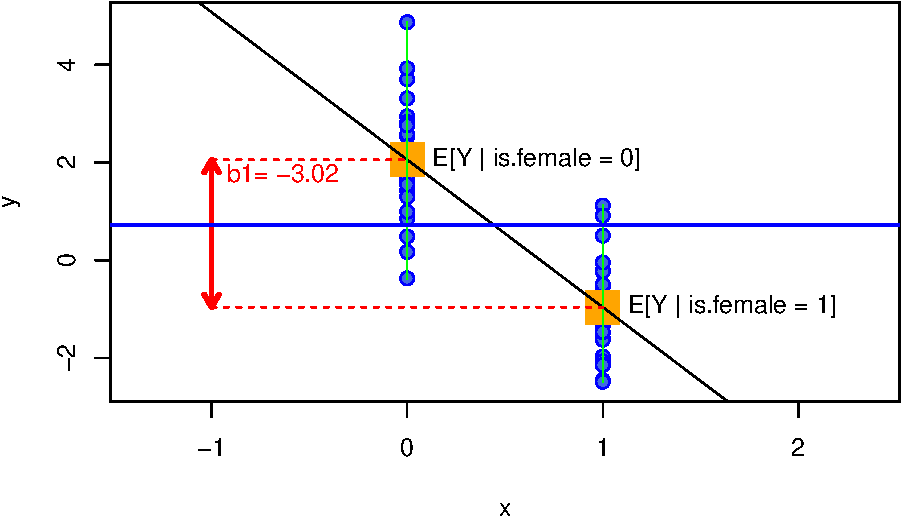
\includegraphics{ScPoEconometrics_files/figure-latex/x-zero-one-1} 

}

\caption{regressing $y \in \mathbb{R}$ on $\text{is.female}_i \in \{0,1\}$. The blue line is $E[y]$, the red arrow is the size of $b_1$. Which is the same as the slope of the regression line in this case and the difference in conditional means!}\label{fig:x-zero-one}
\end{figure}

In figure \ref{fig:x-zero-one} we see that this regression simplifies to
the straight line connecting the mean, or the \emph{expected value} of
\(y\) when \(\text{is.female}_i = 0\), i.e.
\(E[y|\text{is.female}_i=0]\), to the mean when
\(\text{is.female}_i=1\), i.e. \(E[y|\text{is.female}_i=1]\). It is
useful to remember that the \emph{unconditional mean} of \(y\), i.e.
\(E[y]\), is going to be the result of regressing \(y\) only on an
intercept, illustrated by the blue line. This line will always lie in
between both conditional means. As indicated by the red arrow, the
estimate of the coefficient on the dummy, \(b_1\), is equal to the
difference in conditional means for both groups. You should look at our
app now to deepen your understanding of what's going on here:

\begin{Shaded}
\begin{Highlighting}[]
\KeywordTok{library}\NormalTok{(ScPoEconometrics)}
\KeywordTok{launchApp}\NormalTok{(}\StringTok{"reg_dummy"}\NormalTok{)}
\end{Highlighting}
\end{Shaded}

\section{Dummy and Continuous
Variables}\label{dummy-and-continuous-variables}

What happens if there are more predictors than just the dummy variable
in a regression? For example, what if instead we had

\begin{equation}
y_i = b_0 + b_1 \text{is.female}_i + b_2 \text{exper}_i + e_i \label{eq:dummy-reg2}
\end{equation}

where \(\text{exper}_i\) would measure years of experience in the labor
market? As above, the dummy variable acts as an intercept shifter. We
have

\begin{equation}
y_i =  \begin{cases}
b_0 + b_1 + b_2 \times \text{exper}_i + e_i & \text{if is.female=1} \\
b_0  + \hphantom{b_1} +b_2 \times \text{exper}_i + e_i & \text{if is.female=0}
\end{cases}
\end{equation}

so that the intercept is \(b_0 + b_1\) for women but \(b_0\) for men. We
will see this in the real-world example below, but for now let's see the
effect of switching the dummy \emph{on} and \emph{off} in this app:

\begin{Shaded}
\begin{Highlighting}[]
\KeywordTok{library}\NormalTok{(ScPoEconometrics)}
\KeywordTok{launchApp}\NormalTok{(}\StringTok{"reg_dummy_example"}\NormalTok{)}
\end{Highlighting}
\end{Shaded}

\section{\texorpdfstring{Categorical Variables in \texttt{R}:
\texttt{factor}}{Categorical Variables in R: factor}}\label{categorical-variables-in-r-factor}

\texttt{R} has extensive support for categorical variables built-in. The
relevant data type representing a categorical variable is called
\texttt{factor}. We encountered them as basic data types in section
\ref{data-types} already, but it is worth repeating this here. We have
seen that a factor \emph{categorizes} a usually small number of numeric
values by \emph{labels}, as in this example which is similar to what I
used to create regressor \texttt{is.female} for the above regression:

\begin{Shaded}
\begin{Highlighting}[]
\NormalTok{is.female =}\StringTok{ }\KeywordTok{factor}\NormalTok{(}\DataTypeTok{x =} \KeywordTok{c}\NormalTok{(}\DecValTok{0}\NormalTok{,}\DecValTok{1}\NormalTok{,}\DecValTok{1}\NormalTok{,}\DecValTok{0}\NormalTok{), }\DataTypeTok{labels =} \KeywordTok{c}\NormalTok{(}\OtherTok{FALSE}\NormalTok{,}\OtherTok{TRUE}\NormalTok{))}
\NormalTok{is.female}
\end{Highlighting}
\end{Shaded}

\begin{verbatim}
#OUT> [1] FALSE TRUE  TRUE  FALSE
#OUT> Levels: FALSE TRUE
\end{verbatim}

You can see the result is a vector object of type \texttt{factor} with 4
entries, whereby \texttt{0} is represented as \texttt{FALSE} and
\texttt{1} as \texttt{TRUE}. An other example could be if we wanted to
record a variable \emph{sex} instead, and we could do

\begin{Shaded}
\begin{Highlighting}[]
\NormalTok{sex =}\StringTok{ }\KeywordTok{factor}\NormalTok{(}\DataTypeTok{x =} \KeywordTok{c}\NormalTok{(}\DecValTok{0}\NormalTok{,}\DecValTok{1}\NormalTok{,}\DecValTok{1}\NormalTok{,}\DecValTok{0}\NormalTok{), }\DataTypeTok{labels =} \KeywordTok{c}\NormalTok{(}\StringTok{"male"}\NormalTok{,}\StringTok{"female"}\NormalTok{))}
\NormalTok{sex}
\end{Highlighting}
\end{Shaded}

\begin{verbatim}
#OUT> [1] male   female female male  
#OUT> Levels: male female
\end{verbatim}

You can see that this is almost identical, just the \emph{labels} are
different.

\subsection{More Levels}\label{more-levels}

We can go beyond \emph{binary} categorical variables such as
\texttt{TRUE} vs \texttt{FALSE}. For example, suppose that \(x\)
measures educational attainment, i.e.~it is now something like
\(x_i \in \{\text{high school,some college,BA,MSc}\}\). In \texttt{R}
parlance, \emph{high school, some college, BA, MSc} are the
\textbf{levels of factor \(x\)}. A straightforward extension of the
above would dictate to create one dummy variable for each category (or
level), like

\begin{align*}
\text{has.HS}_i &= \mathbf{1}[x_i==\text{high school}] \\
\text{has.someCol}_i &= \mathbf{1}[x_i==\text{some college}] \\
\text{has.BA}_i &= \mathbf{1}[x_i==\text{BA}] \\
\text{has.MSc}_i &= \mathbf{1}[x_i==\text{MSc}] 
\end{align*}

but you can see that this is cumbersome. There is a better solution for
us available:

\begin{Shaded}
\begin{Highlighting}[]
\KeywordTok{factor}\NormalTok{(}\DataTypeTok{x =} \KeywordTok{c}\NormalTok{(}\DecValTok{1}\NormalTok{,}\DecValTok{1}\NormalTok{,}\DecValTok{2}\NormalTok{,}\DecValTok{4}\NormalTok{,}\DecValTok{3}\NormalTok{,}\DecValTok{4}\NormalTok{),}\DataTypeTok{labels =} \KeywordTok{c}\NormalTok{(}\StringTok{"HS"}\NormalTok{,}\StringTok{"someCol"}\NormalTok{,}\StringTok{"BA"}\NormalTok{,}\StringTok{"MSc"}\NormalTok{))}
\end{Highlighting}
\end{Shaded}

\begin{verbatim}
#OUT> [1] HS      HS      someCol MSc     BA      MSc    
#OUT> Levels: HS someCol BA MSc
\end{verbatim}

Notice here that \texttt{R} will apply the labels in increasing order
the way you supplied it (i.e.~a numerical value \texttt{4} will
correspond to ``MSc'', no matter the ordering in \texttt{x}.)

\subsection{Log Wages and Dummies}\label{factors}

The above developed \texttt{factor} terminology fits neatly into
\texttt{R}'s linear model fitting framework. Let us illustrate the
simplest use by way of example.

Going back to our wage example, let's say that a worker's wage depends
on their education as well as their sex:

\begin{equation}
\ln w_i = b_0 + b_1 educ_i + b_2 female_i + e_i \label{eq:wage-sex}
\end{equation}

\begin{Shaded}
\begin{Highlighting}[]
\KeywordTok{data}\NormalTok{(}\StringTok{"wage1"}\NormalTok{, }\DataTypeTok{package =} \StringTok{"wooldridge"}\NormalTok{)}
\NormalTok{wage1}\OperatorTok{$}\NormalTok{female =}\StringTok{ }\KeywordTok{as.factor}\NormalTok{(wage1}\OperatorTok{$}\NormalTok{female)  }\CommentTok{# convert 0-1 to factor}
\NormalTok{lm_w =}\StringTok{ }\KeywordTok{lm}\NormalTok{(lwage }\OperatorTok{~}\StringTok{ }\NormalTok{educ, }\DataTypeTok{data =}\NormalTok{ wage1)}
\NormalTok{lm_w_sex =}\StringTok{ }\KeywordTok{lm}\NormalTok{(lwage }\OperatorTok{~}\StringTok{ }\NormalTok{educ }\OperatorTok{+}\StringTok{ }\NormalTok{female, }\DataTypeTok{data =}\NormalTok{ wage1)}
\NormalTok{stargazer}\OperatorTok{::}\KeywordTok{stargazer}\NormalTok{(lm_w,lm_w_sex,}\DataTypeTok{type =} \ControlFlowTok{if}\NormalTok{ (knitr}\OperatorTok{:::}\KeywordTok{is_latex_output}\NormalTok{()) }\StringTok{"latex"} \ControlFlowTok{else} \StringTok{"html"}\NormalTok{)}
\end{Highlighting}
\end{Shaded}

\% Table created by stargazer v.5.2.2 by Marek Hlavac, Harvard
University. E-mail: hlavac at fas.harvard.edu \% Date and time: Mon, Nov
25, 2019 - 10:11:21 PM

\begin{table}[!htbp] \centering 
  \caption{} 
  \label{} 
\begin{tabular}{@{\extracolsep{5pt}}lcc} 
\\[-1.8ex]\hline 
\hline \\[-1.8ex] 
 & \multicolumn{2}{c}{\textit{Dependent variable:}} \\ 
\cline{2-3} 
\\[-1.8ex] & \multicolumn{2}{c}{lwage} \\ 
\\[-1.8ex] & (1) & (2)\\ 
\hline \\[-1.8ex] 
 educ & 0.083$^{***}$ & 0.077$^{***}$ \\ 
  & (0.008) & (0.007) \\ 
  & & \\ 
 female1 &  & $-$0.361$^{***}$ \\ 
  &  & (0.039) \\ 
  & & \\ 
 Constant & 0.584$^{***}$ & 0.826$^{***}$ \\ 
  & (0.097) & (0.094) \\ 
  & & \\ 
\hline \\[-1.8ex] 
Observations & 526 & 526 \\ 
R$^{2}$ & 0.186 & 0.300 \\ 
Adjusted R$^{2}$ & 0.184 & 0.298 \\ 
Residual Std. Error & 0.480 (df = 524) & 0.445 (df = 523) \\ 
F Statistic & 119.582$^{***}$ (df = 1; 524) & 112.189$^{***}$ (df = 2; 523) \\ 
\hline 
\hline \\[-1.8ex] 
\textit{Note:}  & \multicolumn{2}{r}{$^{*}$p$<$0.1; $^{**}$p$<$0.05; $^{***}$p$<$0.01} \\ 
\end{tabular} 
\end{table}

We know the results from column (1) very well by now. How does the
relationship change if we include the \texttt{female} indicator?
Remember from above that \texttt{female} is a \texttt{factor} with two
levels, \emph{0} and \emph{1}, where \emph{1} means \emph{that's a
female}. We see in the above output that \texttt{R} included a regressor
called \texttt{female1}. This is a combination of the variable name
\texttt{female} and the level which was included in the regression. In
other words, \texttt{R} chooses a \emph{reference category} (by default
the first of all levels by order of appearance), which is excluded -
here this is \texttt{female==0}. The interpretation is that \(b_2\)
measures the effect of being female \emph{relative} to being male.
\texttt{R} automatically creates a dummy variable for each potential
level, excluding the first category.

\begin{figure}

{\centering 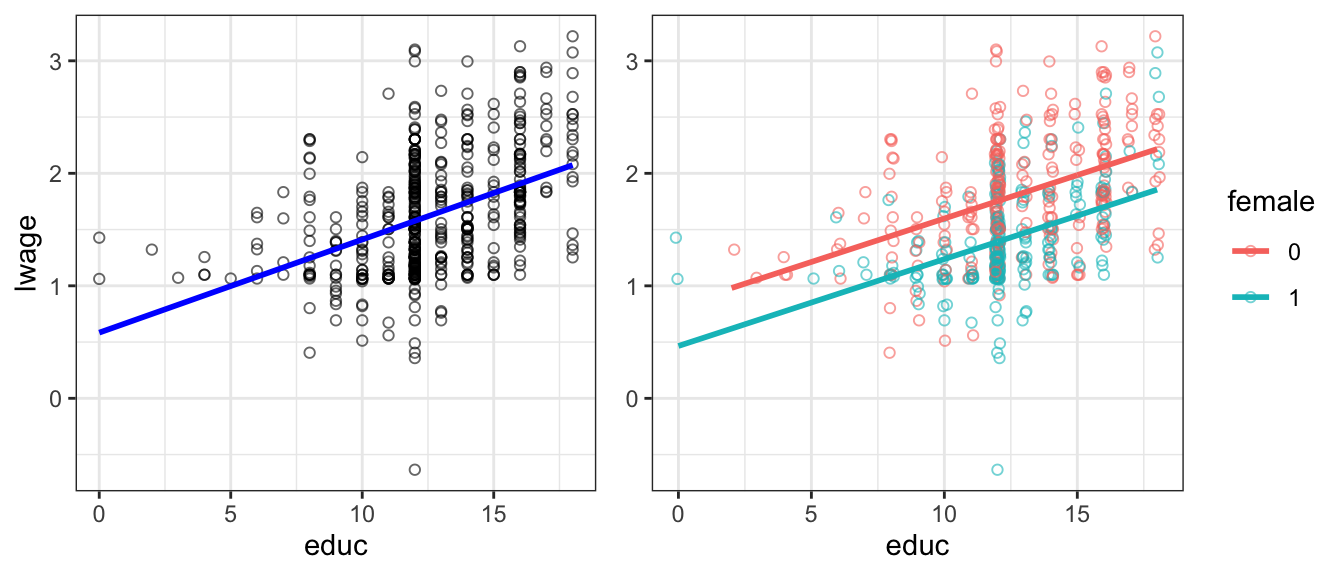
\includegraphics{ScPoEconometrics_files/figure-latex/wage-plot-1} 

}

\caption{log wage vs educ. Right panel with female dummy.}\label{fig:wage-plot}
\end{figure}

Figure \ref{fig:wage-plot} illustrates this. The left panel is our
previous model. The right panel adds the \texttt{female} dummy. You can
see that both male and female have the same upward sloping regression
line. But you can also see that there is a parallel downward shift from
male to female line. The estimate of \(b_2 = -0.36\) is the size of the
downward shift.

\section{Interactions}\label{interactions}

Sometimes it is useful to let the slope of a certain variable to be
dependent on the value of \emph{another} regressor. For example consider
a model for the sales prices of houses, where \texttt{area} is the
livable surface of the property, and \texttt{age} is its age:

\begin{equation}
\log(price) = b_0 + b_1 \text{area} + b_2 \text{age} + b_3 (\text{area} \times \text{age}) + e  \label{eq:price-interact}
\end{equation}

In that model, the partial effect of \texttt{area} on
\texttt{log(price)}, keeping all other variables fixed, is

\begin{equation}
\frac{\partial \log(price)}{\partial \text{area}} = b_1 + b_3 (\text{age}) 
\end{equation}

If we find that \(b_3 > 0\) in a regression, we conclude that the size
of a house values more in older houses. We call \(b_3\) the
\textbf{interaction effect} between area and age. Let's look at that
regression model now.

\begin{Shaded}
\begin{Highlighting}[]
\KeywordTok{data}\NormalTok{(hprice3, }\DataTypeTok{package =} \StringTok{"wooldridge"}\NormalTok{)}
\KeywordTok{summary}\NormalTok{(}\KeywordTok{lm}\NormalTok{(lprice }\OperatorTok{~}\StringTok{ }\NormalTok{area}\OperatorTok{*}\NormalTok{age, }\DataTypeTok{data =}\NormalTok{ hprice3))}
\end{Highlighting}
\end{Shaded}

\begin{verbatim}
#OUT> 
#OUT> Call:
#OUT> lm(formula = lprice ~ area * age, data = hprice3)
#OUT> 
#OUT> Residuals:
#OUT>      Min       1Q   Median       3Q      Max 
#OUT> -1.27226 -0.16538 -0.00298  0.20673  0.83985 
#OUT> 
#OUT> Coefficients:
#OUT>               Estimate Std. Error t value Pr(>|t|)    
#OUT> (Intercept)  1.071e+01  6.633e-02 161.448  < 2e-16 ***
#OUT> area         3.647e-04  2.875e-05  12.686  < 2e-16 ***
#OUT> age         -7.377e-03  1.358e-03  -5.434  1.1e-07 ***
#OUT> area:age     9.168e-07  4.898e-07   1.872   0.0622 .  
#OUT> ---
#OUT> Signif. codes:  0 '***' 0.001 '**' 0.01 '*' 0.05 '.' 0.1 ' ' 1
#OUT> 
#OUT> Residual standard error: 0.2925 on 317 degrees of freedom
#OUT> Multiple R-squared:  0.5586,  Adjusted R-squared:  0.5545 
#OUT> F-statistic: 133.7 on 3 and 317 DF,  p-value: < 2.2e-16
\end{verbatim}

In this instance, we see that indeed there is a small positive
interaction between \texttt{area} and \texttt{age} on the sales price:
even though \texttt{age} in isolation decreases the sales value, bigger
houses command a small premium if they are older.

\subsection{Interactions with Dummies: Differential
Slopes}\label{interactions-with-dummies-differential-slopes}

It is straightforward to extend the interactions logic to allow not only
for different \emph{intercepts}, but also different \emph{slopes} for
each subgroup in a dataset. Let's go back to our dataset of wages from
section \ref{factors} above. Now that we know how to create and
interaction between two variables, we can easily modify equation
\eqref{eq:wage-sex} like this:

\begin{equation}
\ln w = b_0 + b_1 \text{female} + b_2 \text{educ} + b_3 (\text{female} \times \text{educ}) + e \label{eq:wage-sex2}
\end{equation}

The only peculiarity here is that \texttt{female} is a factor with
levels \texttt{0} and \texttt{1}: i.e.~the interaction term \(b_3\) will
be zero for all men. Similarly to above, we can test whether there are
indeed different returns to education or men and women by looking at the
estimated value \(b_3\):

\begin{Shaded}
\begin{Highlighting}[]
\NormalTok{lm_w_interact <-}\StringTok{ }\KeywordTok{lm}\NormalTok{(lwage }\OperatorTok{~}\StringTok{ }\NormalTok{educ }\OperatorTok{*}\StringTok{ }\NormalTok{female , }\DataTypeTok{data =}\NormalTok{ wage1)  }\CommentTok{# R expands to full interactions model}
\KeywordTok{summary}\NormalTok{(lm_w_interact)}
\end{Highlighting}
\end{Shaded}

\begin{verbatim}
#OUT> 
#OUT> Call:
#OUT> lm(formula = lwage ~ educ * female, data = wage1)
#OUT> 
#OUT> Residuals:
#OUT>      Min       1Q   Median       3Q      Max 
#OUT> -2.02673 -0.27468 -0.03721  0.26221  1.34740 
#OUT> 
#OUT> Coefficients:
#OUT>                Estimate Std. Error t value Pr(>|t|)    
#OUT> (Intercept)   8.260e-01  1.181e-01   6.997 8.08e-12 ***
#OUT> educ          7.723e-02  8.988e-03   8.593  < 2e-16 ***
#OUT> female1      -3.601e-01  1.854e-01  -1.942   0.0527 .  
#OUT> educ:female1 -6.408e-05  1.450e-02  -0.004   0.9965    
#OUT> ---
#OUT> Signif. codes:  0 '***' 0.001 '**' 0.01 '*' 0.05 '.' 0.1 ' ' 1
#OUT> 
#OUT> Residual standard error: 0.4459 on 522 degrees of freedom
#OUT> Multiple R-squared:  0.3002,  Adjusted R-squared:  0.2962 
#OUT> F-statistic: 74.65 on 3 and 522 DF,  p-value: < 2.2e-16
\end{verbatim}

We will in the next chapter learn that the estimate for \(b_3\) on the
interaction \texttt{educ:female1} is difficult for us to distinguish
from zero in a statistical sense; Hence for now we conclude that there
are \emph{no} significantly different returns in education for men and
women in this data. This is easy to verify visually in this plot, where
we are unable to detect a difference in slopes in the right panel.

\begin{figure}

{\centering 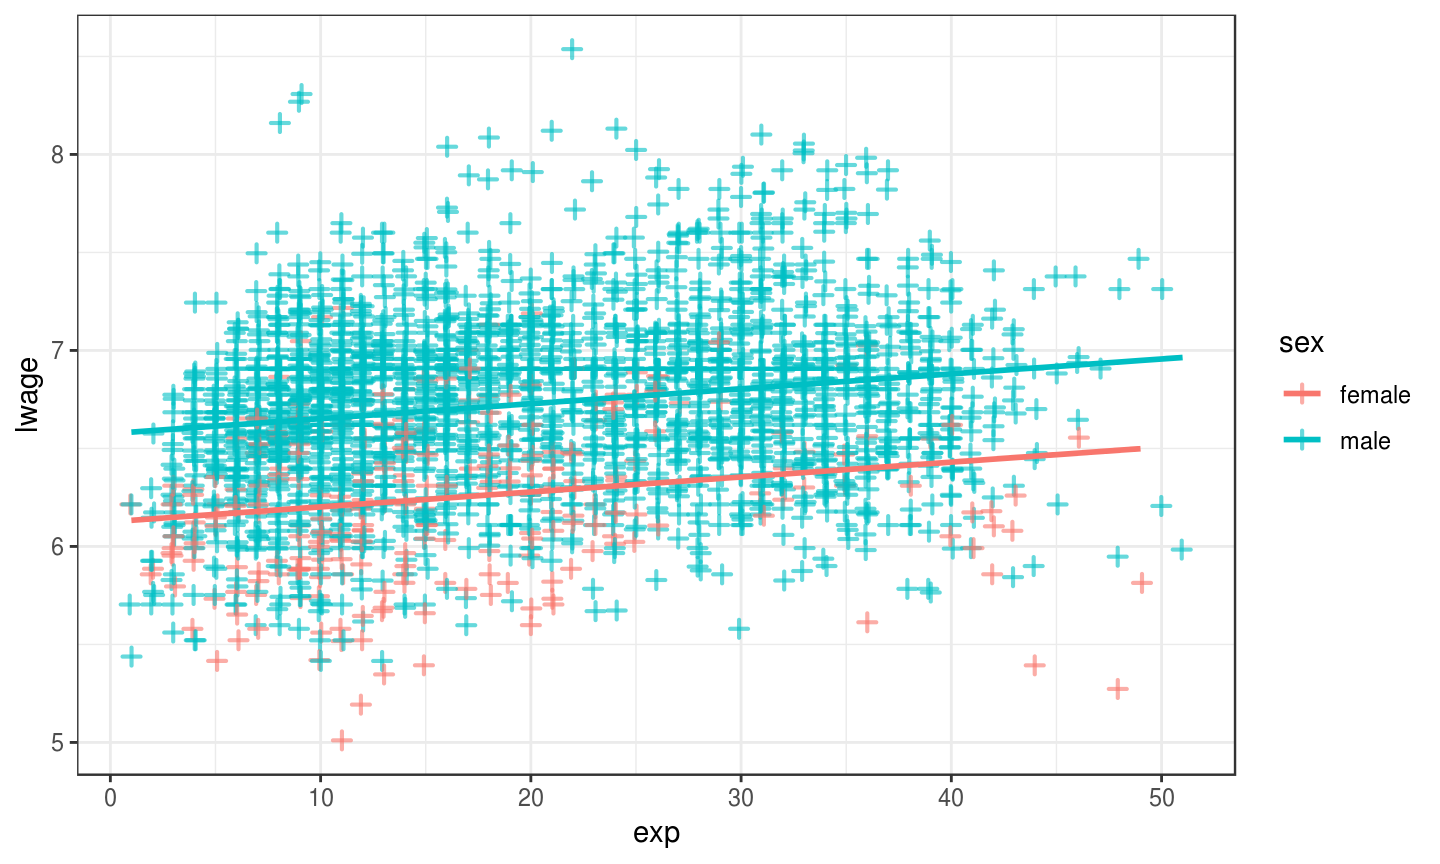
\includegraphics{ScPoEconometrics_files/figure-latex/wage-plot2-1} 

}

\caption{log wage vs educ. Right panel allows slopes to be different - turns out they are not!}\label{fig:wage-plot2}
\end{figure}

\section{(Unobserved) Individual
Heterogeneity}\label{unobserved-individual-heterogeneity}

Finally, dummary variables are sometimes very important to account for
spurious relationships in that data. Consider the following (artificial
example):

\begin{enumerate}
\def\labelenumi{\arabic{enumi}.}
\tightlist
\item
  Suppose we collected data on hourly wage data together with a the
  number of hours worked for a set of individuals.
\item
  We plot want to investigate labour supply behaviour of those
  individuals, hence we run regression
  \texttt{hours\_worked\ \textasciitilde{}\ wage}.
\item
  We expect to get a positive coefficient on \texttt{wage}: the higher
  the wage, the more hours worked.
\item
  You know that individuals are members of either group \texttt{g=0} or
  \texttt{g=1}.
\end{enumerate}

\begin{center}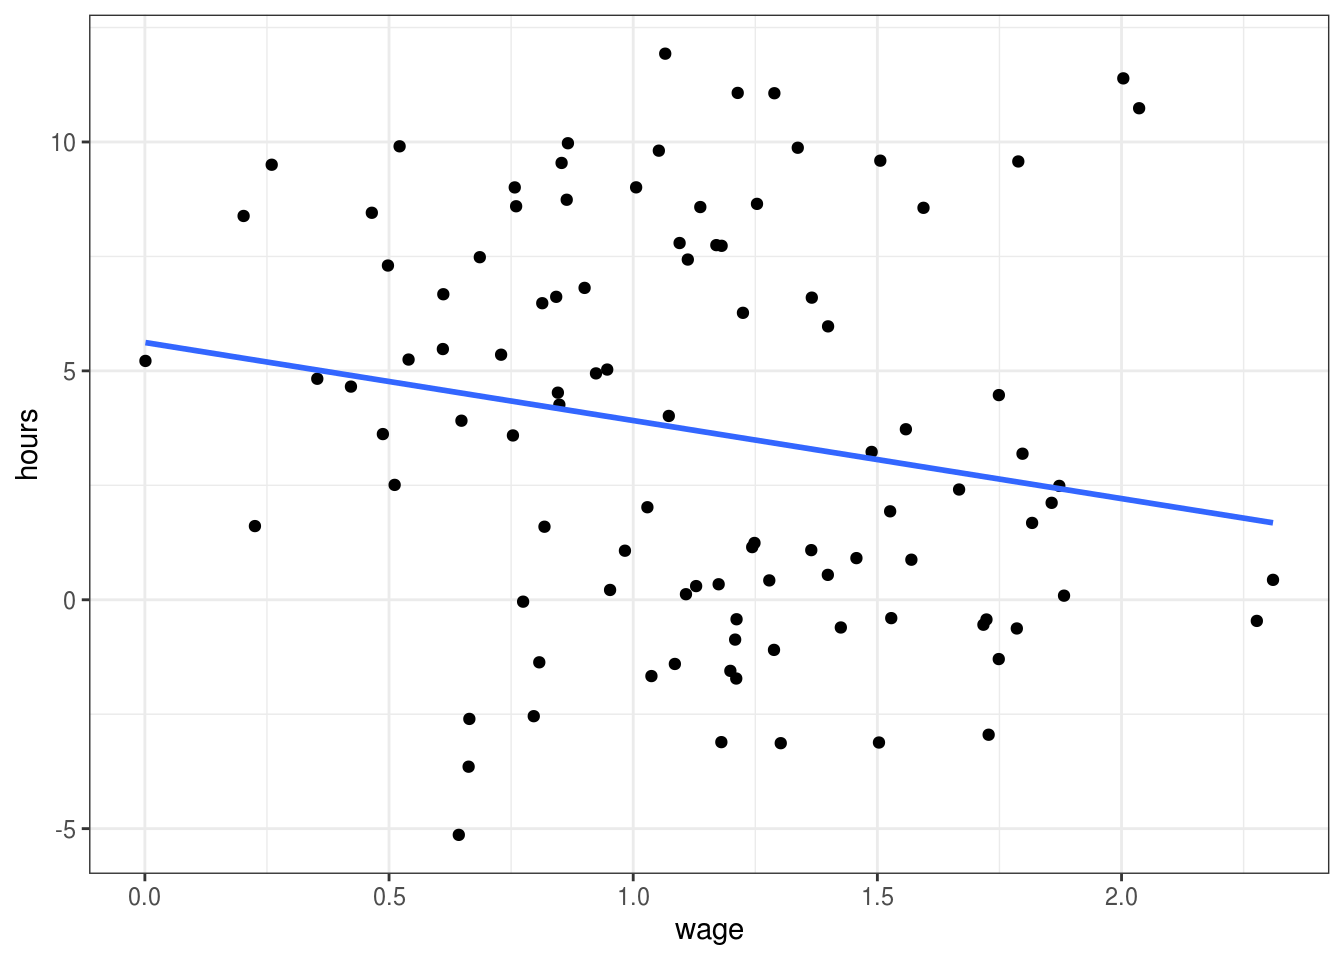
\includegraphics{ScPoEconometrics_files/figure-latex/unnamed-chunk-165-1} \end{center}

Here we observe a slightly negative relationship: higher wages are
associated with fewer hours worked? Maybe. But what is this, there is a
group identifier in this data! Let's use this and include \texttt{g} as
a dummy in the regression - suppose \texttt{g} encodes male and female.

\begin{figure}

{\centering 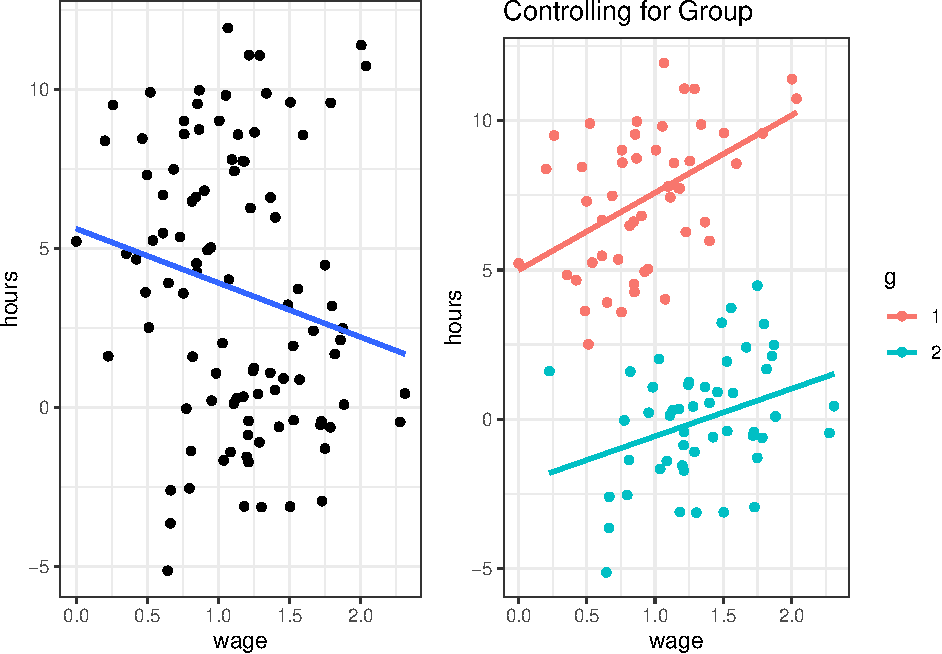
\includegraphics{ScPoEconometrics_files/figure-latex/unnamed-chunk-166-1} 

}

\caption{Left and right panel exhibit the same data. The right panel controls for group composition.}\label{fig:unnamed-chunk-166}
\end{figure}

This is an artificial example; yet it shows that you can be severly
misled if you don't account for group-specific effects in your data. The
problem is particularly accute if we \emph{don't know group membership}
- we can then resort to advanced methods that are beyond the scope of
this course to \emph{estimate} which group each individual belongs to.
If we \emph{do know} group membership, however, it is good practice to
include a group dummy so as to control for group effects.

\chapter{Regression Inference}\label{std-errors}

In this chapter we want to investigate uncertainty in regression
estimates. We want to understand what the precise meaning of the
\texttt{Std.\ Error} column in a typical regression table is telling us.
In terms of a picture, we want to understand better the meaning of the
shaded area as in this one here:

\begin{figure}

{\centering 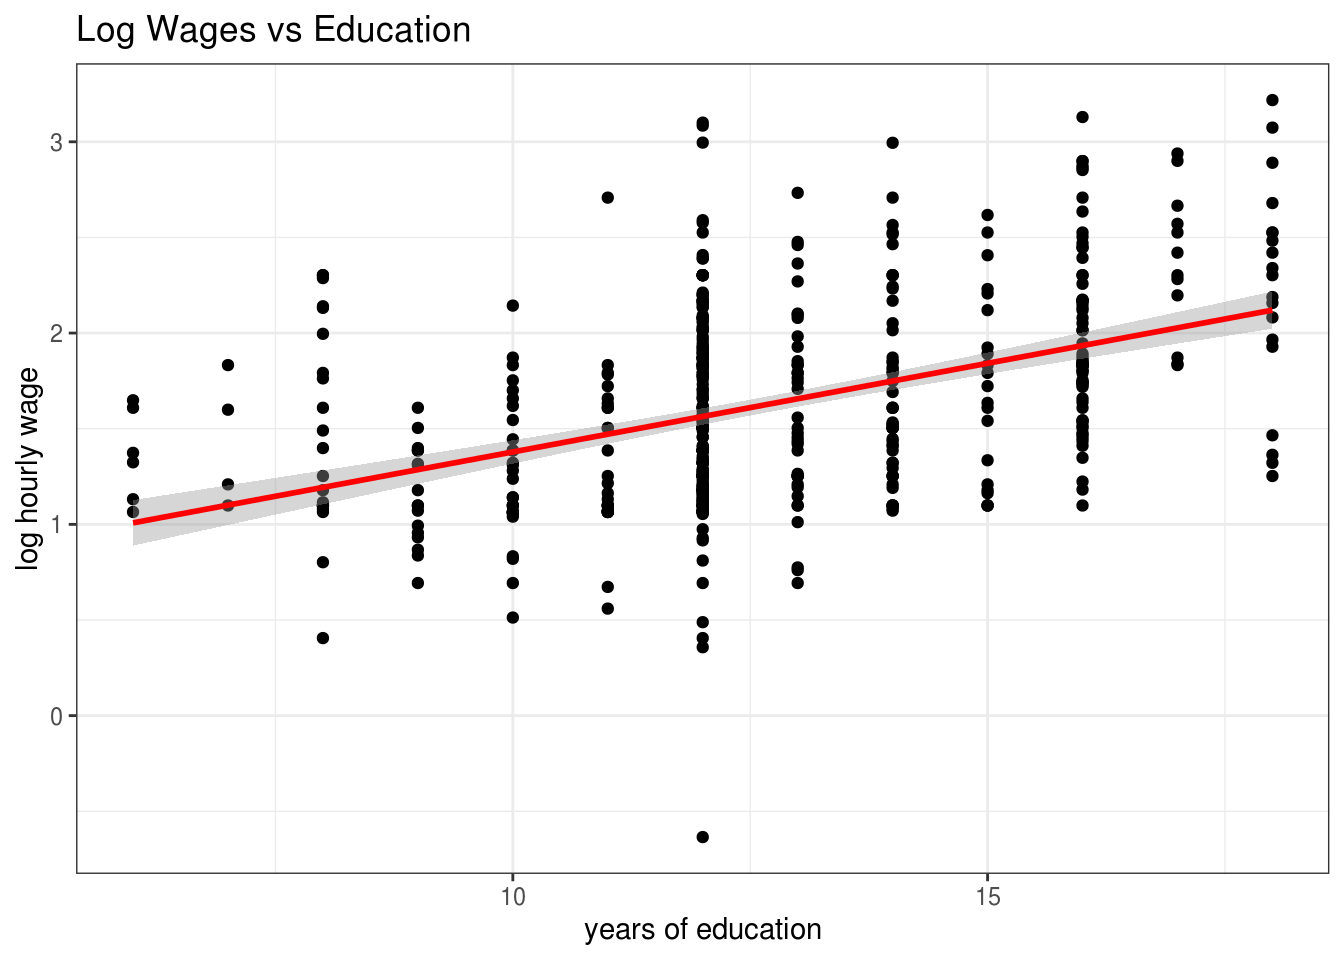
\includegraphics{ScPoEconometrics_files/figure-latex/confint-1} 

}

\caption{Confidence bands around a regression line.}\label{fig:confint}
\end{figure}

In order to fully understand this, we need to go back and make sure we
have a good grasp of \emph{sampling}. Let's do this first.

\section{Sampling}\label{sampling}

In class we were confronted with a jar of Tricolore Fusilli pasta as
picture in figure \ref{fig:pasta1}.\footnote{This part is largely based
  on \href{https://moderndive.com/7-sampling.html}{moderndive}, to which
  I am giving full credit hereby. Thanks for this great idea.} We asked
ourselves a question which, secretly, many of you had asked themselves
at one point in their lives, namely:

\begin{tip}
What is the proportion of \textbf{green} Fusilli in a pack of Tricolore
Fusilli?
\end{tip}

Well, it's time to find out.

\begin{figure}

{\centering 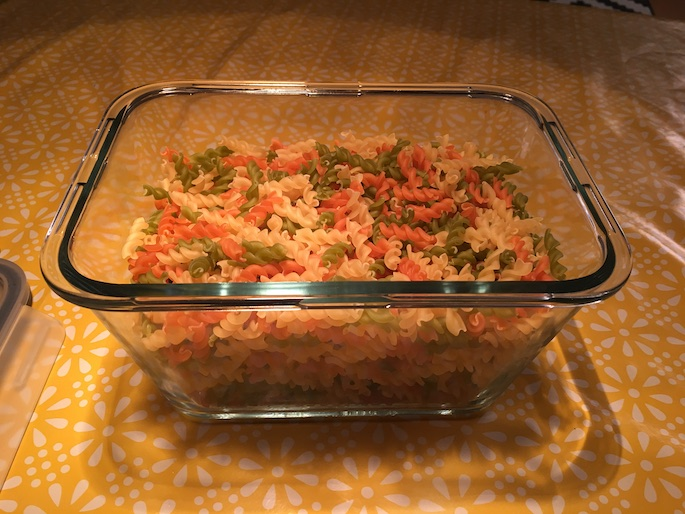
\includegraphics[width=0.9\linewidth]{images/pasta1} 

}

\caption{A glass jar filled with Fusilli pasta in three different colors.}\label{fig:pasta1}
\end{figure}

Let's call the fusilly in this jar our \emph{study population}, i.e.~the
set of units about which we want to learn something. There are several
approaches to address the question of how big a proportion in the
population the green Fusilli make up. One obvious solution is to
enumerate all Fusilli according to their color, and compute their
proportion in the entire population. It works perfectly well as a
solution, but is a long and arduous process, see figures
\ref{fig:pasta2} and \ref{fig:pasta3}.

\begin{figure}

{\centering 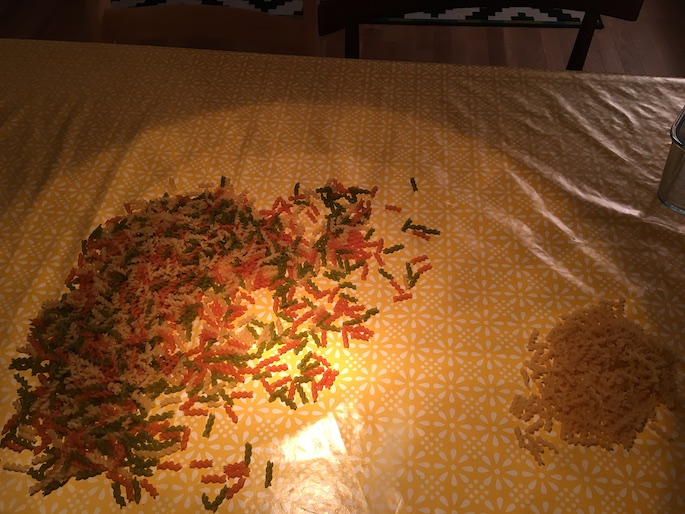
\includegraphics[width=0.9\linewidth]{images/pasta2} 

}

\caption{Manually separating Fusilli by their color is very costly in terms of effort and cost.}\label{fig:pasta2}
\end{figure}

Additionally, you may draw worried looks from the people around you,
while you are doing it. Maybe this is not the right way to approach this
task?\footnote{Regardless of the worried onlookers, I did what I had to
  do and I carried on to count the green pile. I know exactly how many
  greens are in there now! I then computed the weight of 20 Fusilli
  (5g), and backed out the number of Fusilli in the other piles. I will
  declare those numbers as the \emph{true numbers}. (Sceptics are free
  to recount.)}

\begin{figure}

{\centering 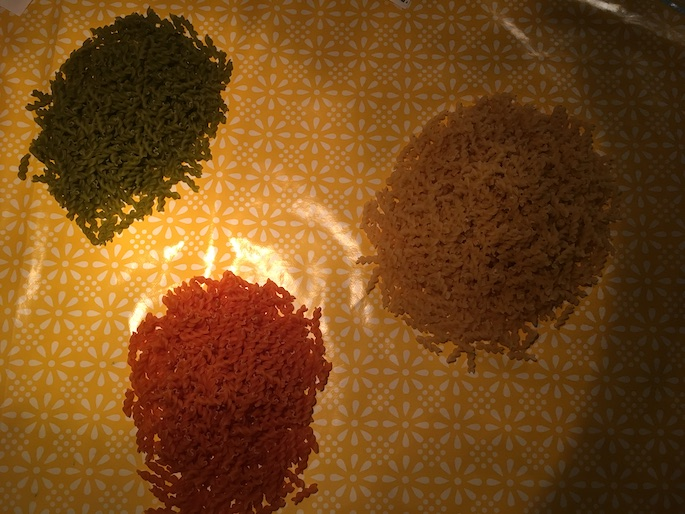
\includegraphics[width=0.9\linewidth]{images/pasta3} 

}

\caption{Heaps of Fusilli pasta ready to be counted.}\label{fig:pasta3}
\end{figure}

\subsection{Taking One Sample From the
Population}\label{taking-one-sample-from-the-population}

We started by randomly grabbing a handful of Fusilli from the jar and by
letting drop exactly \(N=20\) into a paper coffee cup, pictured in
\ref{fig:pasta5}. We call \(N\) the \emph{sample size}. The count and
corresponding proportions of each color in this first sample are shown
in the following table:

\begin{longtable}[]{@{}ccc@{}}
\toprule
Color & Count & Proportion\tabularnewline
\midrule
\endhead
Red & 7 & 0.35\tabularnewline
Green & 5 & 0.25\tabularnewline
White & 8 & 0.4\tabularnewline
\bottomrule
\end{longtable}

So far, so good. We have our first \emph{estimate of the population
proportion of green Fusilli in the overall population}: 0.25. Notice
that taking a sample of \(N=20\) was \emph{much} quicker and \emph{much
less painful} than performing the full count (i.e.~the \emph{census}) of
Fusilli performed above.

\begin{figure}

{\centering 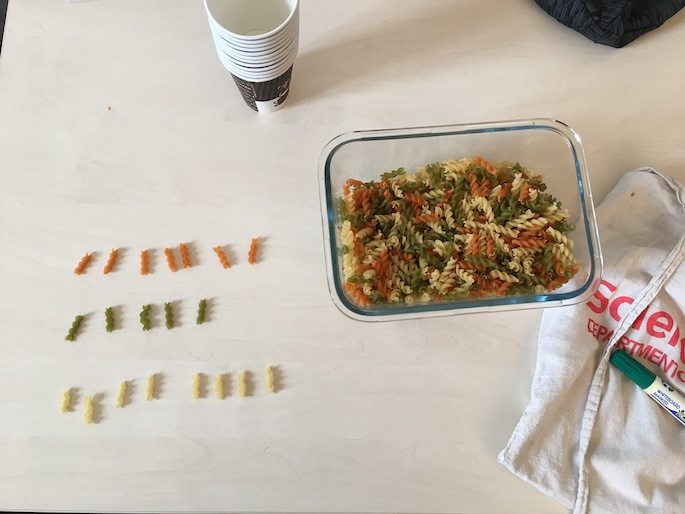
\includegraphics[width=0.9\linewidth]{images/pasta5} 

}

\caption{Taking one sample of 20 Fusilli from the jar.}\label{fig:pasta5}
\end{figure}

Then, we put my sample back into the jar, and we reshuffled the Fusilli.
Had we taken \emph{another} sample, again of \(N=20\), would we again
have gotten 7 Red, 5 Green, and 8 White, just as in the first sample?
Maybe, but maybe not. Suppose we had carried on for several times
drawing samples of 20 and counting the colors: Would we also have
observed 5 green Fusilli? Definitely not. We would have noted some
degree of \emph{variability} in the proportions computed from our
samples. The \emph{sample proportions} in this case are an example of a
\emph{sample statistic}.

\begin{note}
\textbf{Sampling Variation} refers to the fact that if we
\emph{randomly} take samples from a wider population, the \emph{random}
composition of each sample will imply that we obtain statistics that
vary - they take on potentially different values in each sample.
\end{note}

Let's see how this story evolved as we started taking more samples at a
time.

\section{Taking Eleven Samples From The
Population}\label{taking-eleven-samples-from-the-population}

We formed teams of two students in class who would each in turn take
samples from the jar (the population) of size \(N=20\), as before. Each
team computed the proportion of green Fusilli they had in their sample,
and we wrote this data down in a table on the board. Then, we drew a
histogram which showed how many samples had fallen into which bins.

\begin{figure}

{\centering 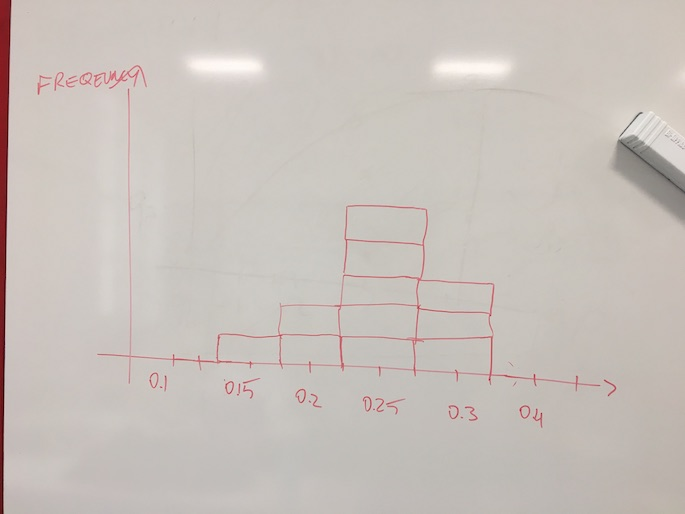
\includegraphics[width=0.9\linewidth]{images/pasta6} 

}

\caption{Taking eleven samples of 20 Fusilli each from the jar, and plotting the histogram of obtained sample proportions of Green Fusilli.}\label{fig:pasta6}
\end{figure}

We looked at the histogram in figure \ref{fig:pasta6} and we noted
several things:

\begin{enumerate}
\def\labelenumi{\arabic{enumi}.}
\tightlist
\item
  The largest proportions where 0.3 green
\item
  The smallest proportion was 0.15 green.
\item
  Most samples found a proportion of 0.25 green fusilli.
\item
  We did think that this looked \emph{suspiciouly} like a \textbf{normal
  distribution}.
\end{enumerate}

We collected the sample data into a data.frame:

\begin{Shaded}
\begin{Highlighting}[]
\NormalTok{pasta_samples <-}\StringTok{ }\KeywordTok{data.frame}\NormalTok{(}\DataTypeTok{group =} \DecValTok{1}\OperatorTok{:}\DecValTok{11}\NormalTok{, }\DataTypeTok{replicate =} \DecValTok{1}\OperatorTok{:}\DecValTok{11}\NormalTok{, }\DataTypeTok{prop_green =} \KeywordTok{c}\NormalTok{(}\FloatTok{0.3}\NormalTok{,}\FloatTok{0.25}\NormalTok{,}\FloatTok{0.25}\NormalTok{,}\FloatTok{0.3}\NormalTok{,}\FloatTok{0.15}\NormalTok{,}\FloatTok{0.3}\NormalTok{,}\FloatTok{0.25}\NormalTok{,}\FloatTok{0.25}\NormalTok{,}\FloatTok{0.2}\NormalTok{,}\FloatTok{0.25}\NormalTok{,}\FloatTok{0.2}\NormalTok{))}
\NormalTok{pasta_samples}
\end{Highlighting}
\end{Shaded}

\begin{verbatim}
#OUT>    group replicate prop_green
#OUT> 1      1         1       0.30
#OUT> 2      2         2       0.25
#OUT> 3      3         3       0.25
#OUT> 4      4         4       0.30
#OUT> 5      5         5       0.15
#OUT> 6      6         6       0.30
#OUT> 7      7         7       0.25
#OUT> 8      8         8       0.25
#OUT> 9      9         9       0.20
#OUT> 10    10        10       0.25
#OUT> 11    11        11       0.20
\end{verbatim}

This produces an associated histogram which looks very much like the one
we draws onto the board:

\begin{center}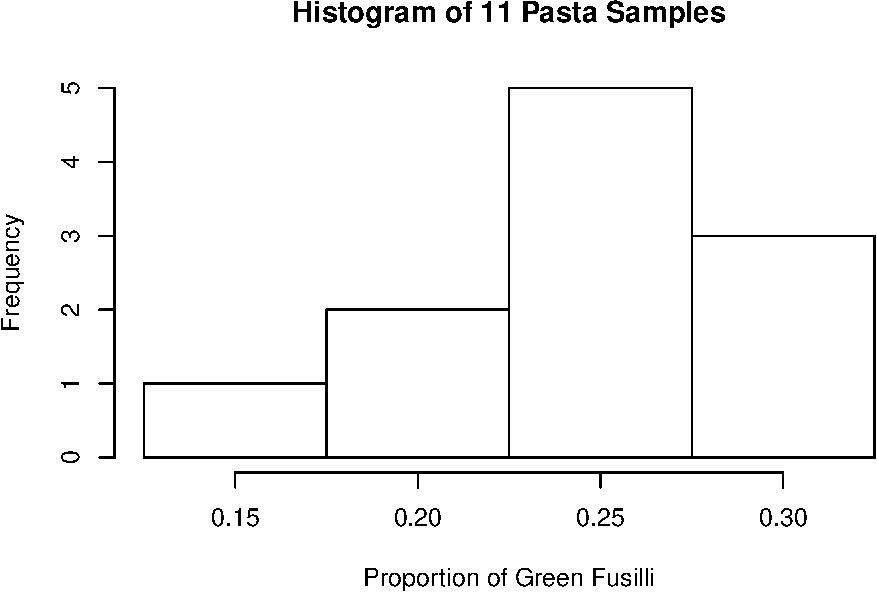
\includegraphics{ScPoEconometrics_files/figure-latex/pasta-hist-1} \end{center}

\subsection{Recap}\label{recap}

Let's recaptiulate what we just did. We wanted to know what proportion
of Fusilli in the glass jar in figure \ref{fig:pasta1} are green. We
acknowledged that an exclusive count, or a census, is a costly and
cumbersome exercise, which in most circumstances we will try to avoid.
In order to make some progress nonetheless, we took a \emph{random
sample} from the full population in the jar: we randomly selected 20
Fusilli, and looked at the proportion of green ones in there. We found a
proportion of 0.25.

After replacing the Fusilli from the first sample in the jar, we asked
ourselves if, upon drawing a \emph{new} sample of 20 Fusilli, we should
expect to see the same outcome - and we concluded: maybe, but maybe not.
In short, we discovered some random variation from sample to sample. We
called this \textbf{sampling variation}.

The purpose of this little activity was three-fold:

\begin{enumerate}
\def\labelenumi{\arabic{enumi}.}
\tightlist
\item
  To understand that random samples differ and that there is sampling
  variation.
\item
  To understand that bigger samples will yield smaller sampling
  variation.
\item
  To illustrate that the sampling distribution of \emph{any} statistic
  (i.e.~not only the sample proportion as in our case) computed from a
  random sample converges to a normal distribution as the sample size
  increases.
\end{enumerate}

\begin{note}
The value of this exercise consisted in making \textbf{you} perform the
sampling activity yourself. We will now hand over to the brilliant
\textbf{moderndive} package, which will further develop this chapter.
\end{note}

\section{\texorpdfstring{Handover to
\texttt{Moderndive}}{Handover to Moderndive}}\label{handover-to-moderndive}

\begin{figure}

{\centering 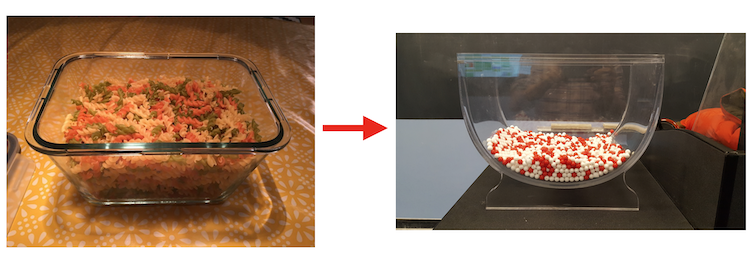
\includegraphics[width=0.9\linewidth]{images/transition} 

}

\caption{The Moderndive package used red and white balls instead of fusilli pasta.}\label{fig:handover}
\end{figure}

The sampling activity in \texttt{moderndive} was performed with red and
white balls instead of green fusilli pasta. The rest is identical. We
will now read sections
\href{https://moderndive.com/7-sampling.html\#sampling-simulation}{7.2}
and
\href{https://moderndive.com/7-sampling.html\#sampling-framework}{7.3}
in their book, as well as
\href{https://moderndive.com/8-confidence-intervals.html}{chapter 8 on
confidence intervals adn bootstrapping}, and
\href{https://moderndive.com/9-hypothesis-testing.html}{chapter 9 on
hypothesis testing}.

\section{Uncertainty in Regression
Estimates}\label{uncertainty-in-regression-estimates}

In the previous chapters we have seen how the OLS method can produce
estimates about intercept and slope coefficients from data. You have
seen this method at work in \texttt{R} by using the \texttt{lm} function
as well. It is now time to introduce the notion that given that \(b_0\),
\(b_1\) and \(b_2\) are \emph{estimates} of some unkown \emph{population
parameters}, there is some degree of \textbf{uncertainty} about their
values. An other way to say this is that we want some indication about
the \emph{precision} of those estimates. The underlying issue that the
data we have at hand are usually \emph{samples} from a larger
population.

\begin{note}
How \emph{confident} should we be about the estimated values \(b\)?
\end{note}

\section{\texorpdfstring{What is \emph{true}? What are Statistical
Models?}{What is true? What are Statistical Models?}}\label{what-is-true-what-are-statistical-models}

A \textbf{statistical model} is simply a set of assumptions about how
some data have been generated. As such, it models the data-generating
process (DGP), as we have it in mind. Once we define a DGP, we could
simulate data from it and see how this compares to the data we observe
in the real world. Or, we could change the parameters of the DGP so as
to understand how the real world data \emph{would} change, could we (or
some policy) change the corresponding parameters in reality. Let us now
consider one particular statistical model, which in fact we have seen so
many times already.

\section{The Classical Regression Model (CRM)}\label{class-reg}

Let's bring back our simple model \eqref{eq:abline} to explain this
concept.

\begin{equation}
y_i = \beta_0 + \beta_1 x_i + \varepsilon_i \label{eq:abline-5}
\end{equation}

The smallest set of assumptions used to define the \emph{classical
regression model} as in \eqref{eq:abline-5} are the following:

\begin{enumerate}
\def\labelenumi{\arabic{enumi}.}
\tightlist
\item
  The data are \textbf{not linearly dependent}: Each variable provides
  new information for the outcome, and it cannot be replicated as a
  linear combination of other variables. We have seen this in section
  \ref{multicol}. In the particular case of one regressor, as here, we
  require that \(x\) exhibit some variation in the data, i.e.
  \(Var(x)\neq 0\).
\item
  The mean of the residuals conditional on \(x\) should be zero,
  \(E[\varepsilon|x] = 0\). Notice that this also means that
  \(Cov(\varepsilon,x) = 0\), i.e.~that the errors and our explanatory
  variable(s) should be \emph{uncorrelated}. It is said that \(x\)
  should be \textbf{strictly exogenous} to the model.
\end{enumerate}

These assumptions are necessary to successfully (and correctly!) run an
OLS regression. They are often supplemented with an additional set of
assumptions, which help with certain aspects of the exposition, but are
not strictly necessary:

\begin{enumerate}
\def\labelenumi{\arabic{enumi}.}
\setcounter{enumi}{2}
\tightlist
\item
  The data are drawn from a \textbf{random sample} of size \(n\):
  observation \((x_i,y_i)\) comes from the exact same distribution, and
  is independent of observation \((x_j,y_j)\), for all \(i\neq j\).
\item
  The variance of the error term \(\varepsilon\) is the same for each
  value of \(x\): \(Var(\varepsilon|x) = \sigma^2\). This property is
  called \textbf{homoskedasticity}.
\item
  The error is normally distributed, i.e.
  \(\varepsilon \sim \mathcal{N}(0,\sigma^2)\)
\end{enumerate}

Invoking assumption 5. in particular defines what is commonly called the
\emph{normal} linear regression model.

\subsection{\texorpdfstring{\(b\) is not
\(\beta\)!}{b is not \textbackslash{}beta!}}\label{b-is-not-beta}

Let's talk about the small but important modifications we applied to
model \eqref{eq:abline} to end up at \eqref{eq:abline-5} above:

\begin{itemize}
\tightlist
\item
  \(\beta_0\) and \(\beta_1\) and intercept and slope parameters
\item
  \(\varepsilon\) is the error term.
\end{itemize}

First, we \emph{assumed} that \eqref{eq:abline-5} is the correct
represenation of the DGP. With that assumption in place, the values
\(\beta_0\) and \(\beta_1\) are the \emph{true parameter values} which
generated the data. Notice that \(\beta_0\) and \(\beta_1\) are
potentially different from \(b_0\) and \(b_1\) in \eqref{eq:abline} for a
given sample of data - they could in practice be very close to each
other, but \(b_0\) and \(b_1\) are \emph{estimates} of \(\beta_0\) and
\(\beta_1\). And, crucially, those estimates are generated from a sample
of data. Now, the fact that our data \(\{y_i,x_i\}_{i=1}^N\) are a
sample from a larger population, means that there will be \emph{sampling
variation} in our estimates - exactly like in the case of the sample
mean estimating the population average as mentioned above. One
particular sample of data will generate one particular set of estimates
\(b_0\) and \(b_1\), whereas another sample of data will generate
estimates which will in general be different - by \emph{how much} those
estimates differ across samples is the question in this chapter. In
general, the more observations we have the greater the precision of our
estimates, hence, the closer the estimates from different samples will
lie together.

\subsection{Violating the Assumptions of the
CRM}\label{violating-the-assumptions-of-the-crm}

It's interesting to consider in which circumstances we might violate
those assumptions. Let's give an example for each of them:

\begin{enumerate}
\def\labelenumi{\arabic{enumi}.}
\item
  No Perfect Collinearity. We have seen that a perfect collinearity
  makes it impossible to compute to OLS coefficients. Remember the
  example about adding \texttt{wtplus\ =\ wt\ +\ 1} to the
  \texttt{mtcars} dataset? Here it is:

\begin{Shaded}
\begin{Highlighting}[]
\KeywordTok{library}\NormalTok{(dplyr)}
\NormalTok{mtcars }\OperatorTok
\KeywordTok{mutate}\NormalTok{(}\DataTypeTok{wtplus =}\NormalTok{ wt }\OperatorTok{+}\StringTok{ }\DecValTok{1}\NormalTok{) }\OperatorTok
\KeywordTok{lm}\NormalTok{(mpg }\OperatorTok{~}\StringTok{ }\NormalTok{wt }\OperatorTok{+}\StringTok{ }\NormalTok{wtplus, }\DataTypeTok{data =}\NormalTok{ .)}
\end{Highlighting}
\end{Shaded}

\begin{verbatim}
#OUT> 
#OUT> Call:
#OUT> lm(formula = mpg ~ wt + wtplus, data = .)
#OUT> 
#OUT> Coefficients:
#OUT> (Intercept)           wt       wtplus  
#OUT>      37.285       -5.344           NA
\end{verbatim}

  That the coefficient on \texttt{wtplus} is \texttt{NA} is the result
  of the direct linear dependence. (Notice that creating
  \texttt{wtplus2\ =\ (wt\ +\ 1)\^{}2}) would work, since that is not
  linear!)
\item
  Conditional Mean of errors is zero, \(E[\varepsilon|x] = 0\). Going
  back to our running example in figure \ref{fig:confint} about wages
  and education: Suppose that each individual \(i\) in our data
  something like \emph{innate ability}, something we might wish to
  measure with an IQ-test, however imperfecty. Let's call it \(a_i\). It
  seems reasonable to think that high \(a_i\) will go together with high
  wages. At the same time, people with high \(a_i\) will find studying
  for exams and school work much less burdensome than others, hence they
  might select into obtaining more years of schooling. The problem?
  Well, there is no \(a_i\) in our regression equation - most of time we
  don't have a good measure of it to start with. So it's an
  \emph{unobserved variable}, and as such, it is part of the error term
  \(\varepsilon\) in our model. We will attribute to \texttt{educ} part
  of the effect on wages that is actually \emph{caused} by ability
  \(a_i\)! Sometimes we may be able to reason about whether our estimate
  on \texttt{educ} is too high or too low, but we will never know it's
  true value. We don't get the \emph{ceteris paribus} effect (the true
  partial derivative of \texttt{educ} on \texttt{lwage}). Technically,
  the assumption \(E[\varepsilon|x] = 0\) implies that
  \(Cov(\varepsilon,x) = 0\), so that's the part that is violated.
\item
  Data from Random Sample. One common concern here is that the
  observations in the data could have been \emph{selected} in a
  particular fashion, which would make it less representative of the
  underlying population. Suppose we had ended up with individuals only
  from the richest neighborhood of town; Our interpretation the impact
  of education on wages might not be valid for other areas.
\item
  Homoskedasticity. For correct inference (below!), we want to know
  whether the variance of \(\varepsilon\) varies with our explanatory
  variable \(x\), or not. Here is a typical example where it does:

  \begin{center}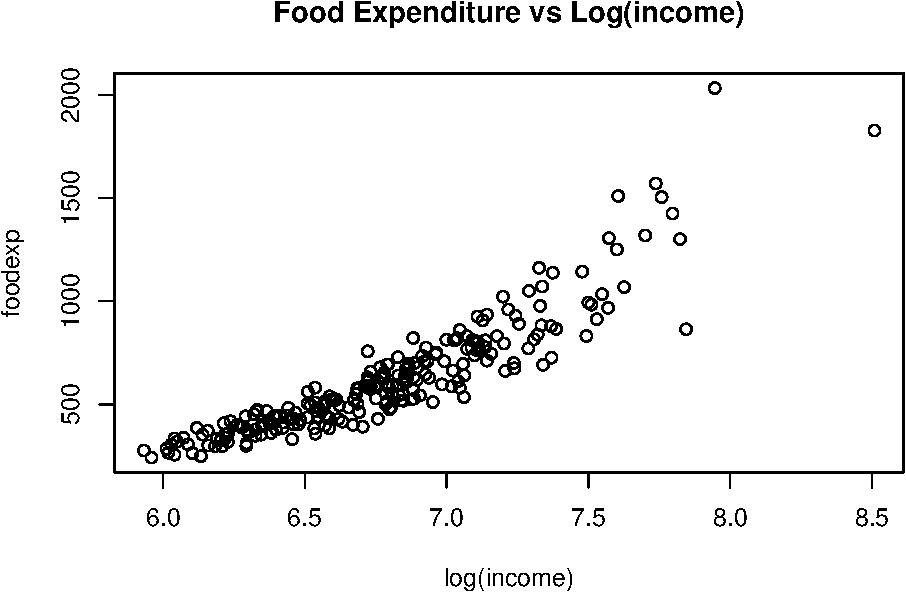
\includegraphics{ScPoEconometrics_files/figure-latex/unnamed-chunk-172-1} \end{center}

  As income increases, not all people increase their food consumption in
  an equal way. So \(Var(\varepsilon|x)\) will vary with the value of
  \(x\), hence it won't be equal to the constant \(\sigma^2\).
\item
  If the distribution of \(\varepsilon\) is not normal, it is more
  cumbersome to derive theoretical results about inference.
\end{enumerate}

\section{Standard Errors in Theory}\label{se-theory}

The standard deviation of the OLS parameters is generally called
\emph{standard error}. As such, it is just the square root of the
parameter's variance. Under assumptions 1. through 4. above we can
define the formula for the variance of our slope coefficient in the
context of our single regressor model \eqref{eq:abline-5} as follows:

\begin{equation}
Var(b_1|x_i) = \frac{\sigma^2}{\sum_i^N (x_i - \bar{x})^2}  \label{eq:var-ols}
\end{equation}

In pratice, we don't know the theoretical variance of \(\varepsilon\),
i.e. \(\sigma^2\), but we form an estimate about it from our sample of
data. A widely used estimate uses the already encountered SSR (sum of
squared residuals), and is denoted \(s^2\):

\[
s^2 = \frac{SSR}{n-p} = \frac{\sum_{i=1}^n (y_i - b_0 - b_1 x_i)^2}{n-p} =  \frac{\sum_{i=1}^n e_i^2}{n-p}
\] where \(n-p\) are the \emph{degrees of freedom} available in this
estimation. \(p\) is the number of parameters we wish to estimate (here:
1). So, the variance formula would become

\begin{equation}
Var(b_1|x_i) = \frac{SSR}{(n-p)\sum_i^N (x_i - \bar{x})^2}  \label{eq:var-ols2}
\end{equation}

We most of the time work directly with the \emph{standard error} of a
coefficient, hence we define

\begin{equation}
SE(b_1) = \sqrt{Var(b_1|x_i)} = \sqrt{\frac{SSR}{(n-p)\sum_i^N (x_i - \bar{x})^2}}  \label{eq:SE-ols2}
\end{equation}

You can clearly see that, as \(n\) increases, the denominator increases,
and therefore variance and standard error of the estimate will decrease.

\chapter{Causality}\label{causality}

In this chapter we take on a challenging part of our course. Remember
that in the
\href{https://rawcdn.githack.com/ScPoEcon/ScPoEconometrics-Slides/session2_1/chapter1/chapter1.html}{first
set of slides} we introduced Econometrics as the economist's toolkit to
answer questions like \emph{does \(x\) \textbf{cause} \(y\)?} Let's
illustrate the issues at stake with a question from epidemiologie and
public health:

\begin{warning}
Does smoking \textbf{cause} lung cancer?
\end{warning}

Just in case you were wondering: Yes it does! However, for a very long
time the \emph{causal impact} of smoking on lung cancer was hotly
debated, and it's instructive for us to look at this history.\footnote{This
  chapter is drawn from chapter 5 of \emph{The Book of Why} by
  \href{http://bayes.cs.ucla.edu/jp_home.html}{Judea Pearl}.}

Let's go back to the 1950's. We are at the start of a big increase in
deaths from lung cancer. At the same time cigarette consumption was
growing very fast. With the benefit of hindsight, we can now draw this
graph:

\begin{figure}

{\centering 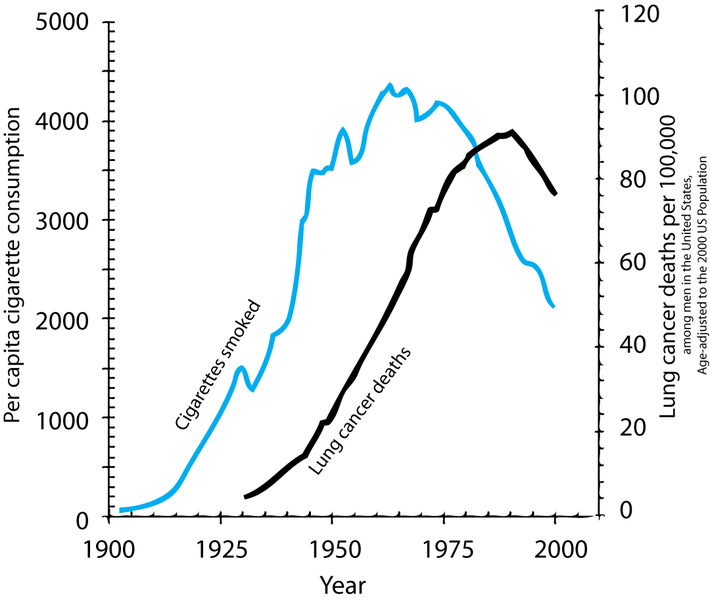
\includegraphics[width=9.86in]{images/Smoking_lung_cancer} 

}

\caption{Two time series showing cigarette consumption per capita and incidence of lung cancer in the USA.}\label{fig:smoking-cancer}
\end{figure}

However, time series graphs are poor tools to make causal statements.
Many \emph{other things} had changed from 1900 to 1950, all of which
could equally be responsible for the rise in cancer rates:

\begin{enumerate}
\def\labelenumi{\arabic{enumi}.}
\tightlist
\item
  Tarring of roads
\item
  Inhalation of motor exhausts (leaded gasoline fumes)
\item
  General greater air pollution.
\end{enumerate}

We call those other factors \textbf{confounders} of the relationship
between smoking and lung cancer.

So, there were a series of sceptics around who at the time were
contesting the existing evidence. That evidence consisted in general of
the following:

\begin{enumerate}
\def\labelenumi{\arabic{enumi}.}
\tightlist
\item
  \textbf{Case-Control studies}: British Epidemiologists Richard Doll
  and Austin Bradford Hill started to compare people already diagnosed
  with cancer to those without, recording their history, and observable
  characteristics (like age and health behaviours). In one study, out of
  649 lung cancer patients interviewed, all but 2 had been smokers! In
  that study, a cancer patient was 1.5 million times more likely to be
  have been a smoker than a non-smoker. Still, critics said, there are
  several sources of bias:

  \begin{itemize}
  \tightlist
  \item
    Hospital patients could be a selected sample of the general
    (smoking) population.
  \item
    Patients could suffer from \emph{recall bias}, affecting their
    recollection of facts.
  \item
    So, while comparing cancer patients to non-patients and controlling
    for several important \emph{confounders} (like age, income and other
    observable characteristics), there was still scope for bias.
  \item
    Moreoever, replicating those studies, as Doll and Hill attempted,
    would not have solved this issue.
  \end{itemize}
\item
  Next they attempted what doctors call a \textbf{Dose-Response Effect}
  study. In 1951 they sent out 60,000 questionnaires to British
  physicians asking about \emph{their} smoking habits. Then they
  followed them over time:

  \begin{itemize}
  \tightlist
  \item
    Only 5 years on, heavy smokers had a death rate from lung cancer
    that was 24 times higher than for nonsmokers.
  \item
    People who had smoked and then stopped reduced their risk by a
    factor of 2.
  \item
    Still, notorious sceptics like R.A. Fisher were unconvinced. The
    studies \emph{still} failed to compare \textbf{otherwise identical}
    smokers to non-smokers. There were \emph{still} important unobserved
    confounders out there which could invalidate the conclusion that we
    observed indeed a \textbf{causal} relationship.
  \end{itemize}
\end{enumerate}

Let's put a some structure on this problem now, so we can make progress.

\section{Directed Acyclical Graphs (DAG)}\label{dags}

A DAG is a tool to visualize a causal relationship. It is a graph where
nodes are connected via arrows, where an arrow can run in one direction
only (hence, \emph{directed} graph). If an arrow starts at node \(x\)
and ends at node \(y\), we say that \(x\) causes \(y\). Here is a simple
example of such a DAG:

\begin{figure}

{\centering \includegraphics{ScPoEconometrics_files/figure-latex/dag1-1} 

}

\caption{A simple DAG showing the causal impact of $x$ on $y$.}\label{fig:dag1}
\end{figure}

Now consider this setting, where there is a third variable, \(z\). It
could be possible that also \(z\) has a direct influence on \(y\):

\begin{figure}

{\centering \includegraphics{ScPoEconometrics_files/figure-latex/dag2-1} 

}

\caption{A simple DAG with with 2 causal paths: Both $x$ and $z$ have a direct impact on $y$.}\label{fig:dag2}
\end{figure}

Now let's change this and create a path from \(z\) to \emph{both} \(x\)
and \(y\) instead. We call \(z\) a \emph{confounder} in the relationship
between \(x\) and \(y\): \(z\) \emph{confounds} the direct causal impact
of \(x\) on \(y\), by affecting them both at the same time. What is
more, there is no arrow from \(x\) to \(y\) at all, so the only
\emph{real} explanatory variable here is in fact \(z\). Attributing any
explanatory power to \(x\) would be wrong in this setting.

\begin{figure}

{\centering \includegraphics{ScPoEconometrics_files/figure-latex/dag3-1} 

}

\caption{A simple DAG where $z$ is a confounder. There is no causal path from $x$ to $y$, and any correlation we observe between those variables is completely induced by $z$. We call this spurious correlation.}\label{fig:dag3}
\end{figure}

Here is a second example where \(z\) is a confounder, but slightly
different.

\begin{figure}

{\centering \includegraphics{ScPoEconometrics_files/figure-latex/dag41-1} 

}

\caption{$z$ is still a confounder here, but there is a causal link from $x$ to $y$ now. If we observed $z$, we can control for it.}\label{fig:dag41}
\end{figure}

In \ref{fig:dag41} there is an arrow from \(x\) to \(y\). In this
setting, if we are able to \emph{observe} \(z\), we can adjust the
correlation we observe between \(x\) to \(y\) for the variation induced
by \(z\). In practice, this is precisely what multiple regression will
do: holding \(z\) fixed at some value, what is the partial effect of
\(x\) on \(y\). Notice that \(z\) cedes to be a confounder in this
situation, and interpreting our regression coefficient on \(x\) as
\emph{causal} is correct.

\section{Smoking in a DAG}\label{smoking-in-a-dag}

Let's use this and cast our problem as a DAG now. What the scientists in
the 1950s faced where two competing models of the relationship between
smoking and lung cancer:

\begin{figure}

{\centering \includegraphics{ScPoEconometrics_files/figure-latex/dag-cig-1} 

}

\caption{Two competing causal graphs for the relationship between smoking and lung cancer. In the right panel Lung Cancer is directly impacted by a genetic factor, which at the same time also influences smoking. This is a stark representation of Fisher's view. Another version would have an additional arrow from Smoking to Lung Cancer in the right panel.}\label{fig:dag-cig}
\end{figure}

Basically, what critics like Fisher were claiming was that the existing
studies did not compare like for like. In other words, our \emph{ceteris
paribus} assumption was not satisfied. They were worried that
\emph{smoking} was not the only relevant difference between a population
of smokers and one of non-smokers. In particular, they worried that
people \textbf{self-selected} into smoking, and that the choice to
become a smoker may be influenced by other, unobserved, underlying
forces - like genetic predisposition, for example. That could mean that
smokers were also more likely to take risks, or more likely to be heavy
drinkers, or engage in other behaviours that might be conducive to
develop lung cancer. They did not formulate it in terms of genetics at
the time, because they could not know until the 2000's, when the human
genome was sufficiently mapped to establish this fact (and indeed there
\textbf{is} a smoking gene! But that's beside the point), but they
worried about this factor.

The argument was settled in the eyes of most physicians, when Jerome
Cornfield in 1959 wrote a rebuttal of Fisher's points. Cornfield's
strategy was to allow Fisher to have his unobserved factor, but to show
that there was an upper bound to \emph{how important} it could be in
determining the outcome. Here goes:

\begin{enumerate}
\def\labelenumi{\arabic{enumi}.}
\tightlist
\item
  Suppose there is indeed a confounding factor ``smoking gene'', and
  that it completely determines the risk of cancer in smokers.
\item
  Suppose smokers are observed to have 9 times the risk of non-smokers
  to develop lung cancer.
\item
  The smoking gene needs to be at least 9 times more prevalent in
  smokers than in non-smokers to explain this difference in risk.
\end{enumerate}

But now consider what this implies. Let's suppose that around 11\% of
all non-smokers have the smoking gene. That means that
\(9\times 11 = 99\%\) of smokers need to have it! What's even more
worrying, if only even 12\% of non smokers have the gene, then the
argument breaks down because it would require \(9\times 12 = 108\%\) of
smokers to have it, which is of course impossible.

This argument was so important that it got a name: \textbf{Cornfield's
inequality}. It left of Fisher's argument nothing but a pile of rubble.
It's impossible to think that genetic variation alone could be so
important in determining a complex choice of becoming a smoker or not.
Looking back at the right panel of figure \ref{fig:dag-cig}, the link
from smoking to lung cancer was much too strong to be explained by the
genetic hypothesis alone.

\section{Randomized Control Trials (RCT) Primer}\label{rct}

We now present a quick introduction to Randomized Control Trials (RCTs).
The history of randomization is fascinating and goes back a long time,
again involving R.A. Fisher from above.\footnote{I refer the interested
  student to the introduction of the \emph{potential outcomes model} of
  \href{https://twitter.com/causalinf}{Scott Cunningham's}
  \href{http://scunning.com/cunningham_mixtape.pdf}{mixtape}, which
  heavily influences this section.} Suffice it to say that RCTs have
become so important in Economics that the
\href{https://www.nobelprize.org/prizes/economic-sciences/2019/summary/}{Nobel
Price in Economics 2019} has been awarded to three exponents of the RCT
literature,
\href{https://www.economist.com/finance-and-economics/2019/10/17/a-nobel-economics-prize-goes-to-pioneers-in-understanding-poverty}{Duflo,
Banerje and Kremer}. RCTs are widely used in Medicine, where they
originate from (in some sense). But, what \emph{are} RCTs?

\begin{note}
A randomized controlled trial is a type of scientific experiment that
aims to reduce certain sources of bias when testing the effectiveness of
some intervention (treatment or policy); this is accomplished by
randomly allocating subjects to two or more groups, treating them
differently, and then comparing them with respect to a measured
response.
\end{note}

 That sounds really intuitive. If we \emph{randomly} allocate people to
receive treatment, there can be no concern of unobserved confounders, as
we have relieved the subjects of making the choice to get treated.
Remember the cigarette smokers above: The concern was that an unobserved
genetic predisposition correlated with both choosing to become a smoker
but also with other potentially cancer-inducing behaviours like drinking
or risk taking. Imagine for a moment that we could randomly select
people at some young age to be selected for treatment (smoking for 30
years, say). The genetic predisposition will be equally prevalent in
both treatment and control group. However, only the treatment group is
allowed (and indeed forced) to smoke. Observing higher cancer rates in
the treatment group would provide \emph{causal evidence} for the effect
of smoking on lung cancer.

Thankfully, such an experiment is impossible to run on ethical grounds.
We could never subject individuals to such severe and prolongued health
risks for the sake of a research study. That's why the question took to
long to be settled!

Let's introduce a formal framework now to think more about RCTs.

\section{The Potential Outcomes Model}\label{rubin}

The Potential Outcomes Model, often named after one of it's inventors
the \emph{Rubin Causal Model}, posits that there are two states of the
world - the \emph{potential outcomes}. A first state, where a certain
intervention is administered to an individual, and a second state, where
this is not the case. Formally, this idea is expressed with superscripts
0 and 1, like this:

\begin{itemize}
\tightlist
\item
  \(Y_i^1\): individual \(i\) has been treated
\item
  \(Y_i^0\): individual \(i\) has \textbf{not} been treated
\end{itemize}

Denoting with \(D_i \in \{0,1\}\) the treatment indicator which is one
if \(i\) is indeed treated, the \emph{observed outcome} \(Y_i\) is then

\begin{equation}
Y_i = D_i Y_i^1 + (1-D_i)Y_i^0 \label{eq:rubin-model}
\end{equation}

This simple equation is able to formalize a rather deep question. We
only ever observe one outcome of events for a given individual \(i\),
say \(Y_i = Y_i^1\) in case treatment was given. The deep question is:
\emph{what would have happened to \(i\), had they \textbf{not} received
treatment}? You will realize that this a very natural question for us
humans to put to ourselves, and to subsequently answer:

\begin{itemize}
\tightlist
\item
  How long would the trip have taken, had I chosen another metro line?
\item
  What would have happened, had I chosen to study a different subject?
\item
  What would have happend, had
  \href{https://en.wikipedia.org/wiki/Neo_(The_Matrix)}{Neo} taken the
  blue pill instead?
\end{itemize}

Our ability to make those considerations distinguishes us from animals.
It's one of the biggest challenges for machines when trying to be
\emph{intelligent}.

What makes this question so hard to answer for machines and animals
alike is the fact that one has to \emph{imagine a parallel universe}
where the actions taken were different, \textbf{without} having observed
that precise situation before. Neo did \emph{not} take the blue pill,
and whatever happened after that originated from this decision - so how
are we to tell what would have happened? It's easy for us and
\href{https://www.quantamagazine.org/to-build-truly-intelligent-machines-teach-them-cause-and-effect-20180515/}{still
hard for machines}.

Potential outcome \(Y_i^0\) above is what is known as the
\emph{counterfactual} outcome. What would have happened to subject
\(i\), had they \textbf{not} received treatment \(D\)?

Following Rubin, let us define the \textbf{treatment effect} for
individual \(i\) as follows:

\begin{equation}
\delta_i = Y_i^1 - Y_i^0 \label{eq:TE}
\end{equation}

Notice our insistence about talking about a single individual \(i\)
throughout here. Keeping the potential outcome model
\eqref{eq:rubin-model} in mind, i.e.~the fact that we only observe
\emph{one} of both outcomes, we face the \textbf{fundamental
identification problem of program evaluation}:

\begin{warning}
Given we only observe \emph{one} potential outcome, we cannot compute
the treatment effect \(\delta_i\) for any individual \(i\).
\end{warning}

 That's pretty dire news. Let's see if we can do better with an average
effect instead. Let's define three \emph{average} effects of interest:

\begin{enumerate}
\def\labelenumi{\arabic{enumi}.}
\tightlist
\item
  the Average Treatment Effect (ATE):
  \[\delta^{ATE} = E[\delta_i] = E[Y_i^1] - E[Y_i^0]\]
\item
  the Average Treatment on the Treated (ATT):
  \[\delta^{ATT} = E[\delta_i|D_i = 1] = E[Y_i^1|D_i = 1] - E[Y_i^0|D_i = 1]\]
\item
  the Average Treatment on the Untreated (ATU):
  \[\delta^{ATU} = E[\delta_i|D_i = 0] = E[Y_i^1|D_i = 0] - E[Y_i^0|D_i = 0]\]
\end{enumerate}

Notice that \emph{none} of those can be computed from data either,
because all of them require data on individual \(i\) from \emph{both}
scenarios. Let's focus on the ATE for now. Fundamentally we face a
\textbf{missing data problem}: either \(Y_i^1\) or \(Y_i^0\) are missing
from our dataset. Nevertheless, let's setup the following \emph{naive}
simple difference in means estimator \(\hat{\delta}\):

\begin{align}
\hat{\delta} =& E[Y_i^1|D_i = 1] - E[Y_i^0|D_i = 0]\\
             =& \frac{1}{N_T} \sum_{i \in T}^{N_T} T_i - \frac{1}{N_C} \sum_{j \in T}^{N_C} Y_j \label{eq:SDO}
\end{align}

in other words, we just difference the mean outcomes in both treatment
(T) and control (C) groups. That is, \(N_C\) is the number of people in
the control group, \(N_T\) is the same for treatment group.

Now let's consider what randomly choosing people for treatment does. The
key consideration here is that the true \(\delta_i\) is potentially
different for each person. That is, some people will have a high effect
of treatment, while others may have a small (or even negative!) effect.
To learn about the true \(\delta^{ATE}\) from our naive
\(\hat{\delta}\), it matters who ends up being treated!

Imagine that individuals have at least some partial knowledge about
their likely \emph{gains from treatment}, i.e.~their personal
\(\delta_i\). If those who expect to benefit a lot will select
disproportionately into treatment, then our estimator \(\hat{\delta}\)
will be biased upwards for the true average effect \(\delta^{ATE}\).
This is so because the average of observed outcomes in the treatment
group, i.e.

\[
\frac{1}{N_T} \sum_{i \in T}^{N_T} Y_i
\]

will be \textbf{too high}. It represents the disproportionately
\emph{high} treatment outcome \(Y_i^1\) for all those who
\emph{anticipated} such a high outcome from treatment, and who therefore
were particularly eager to get selected into treatment. It's not
\emph{representative} of the true population wide treatment outcome
\(E[Y_i^1]\).

Here is where randomization comes into play. Suppose we now flip a coin
for each person to determine whether they obtain treatment or not. This
takes away from them the possibility to select on expected gains into
treatment. Crucially, the distribution of effects \(\delta_i\) is still
the same in the study population, i.e.~there are still people with high
and people with low effects. But we have solved the missing data problem
mentioned above, because whether \(Y_i^1\) or rather \(Y_i^0\) is
observed for each \(i\) is now \textbf{random}, and no longer a function
of any other factor that \(i\) could act upon! Hooray!

Notice how this links back to our initial discussion about DAGs above.
Randomisation essentially cancels the links starting at confounder \(z\)
in \ref{fig:dag41}.

\section{Omitted Variable Bias and
DAGs}\label{omitted-variable-bias-and-dags}

We want to revisit the underlying assumptions of the classical model
outlined in \ref{class-reg} in the previous chapter, which is closely
related to the previous discussion. Let's talk a bit more about
assumption number 2 of the definition in \ref{class-reg}. It said this:

\begin{warning}
The mean of the residuals conditional on \(x\) should be zero,
\(E[\varepsilon|x] = 0\). This means that \(Cov(\varepsilon,x) = 0\),
i.e.~that the errors and our explanatory variable(s) should be
\emph{uncorrelated}. We want \(x\) to be \textbf{strictly exogenous} to
the model.
\end{warning}

Let us start again with

\begin{equation}
y_i = \beta_0 + \beta_1 x_i + \varepsilon_i \label{eq:DGP-h}
\end{equation}

and imagine it represents the data generating process (DGP) of the
impact of \(x\) on \(y\). Writing down this equation is tightly linked
to drawing this DAG from above:

\begin{figure}

{\centering \includegraphics{ScPoEconometrics_files/figure-latex/dag4-1} 

}

\caption{The same simple DAG showing the causal impact of $x$ on $y$.}\label{fig:dag4}
\end{figure}

The role of \(\varepsilon_i\) in equation \eqref{eq:DGP-h} is to allow for
random variability in the data not captured by our model, almost as an
acknowledgement that we would never be able to \emph{fully} explain
\(y_i\) with our necessarily simple model. However, assumption
\(E[\varepsilon|x] = 0\) (or \(Cov(\varepsilon,x) = 0\)) makes sure that
those other factors are in \textbf{no systematic relationship} with our
regressor \(x\). Why? Well if it \emph{were} the case that another
factor \(z\) is related to \(x\), we could never make our ceteris
paribus statements of \emph{holding all other factors fixed, the impact
of \(x\) on \(y\) is \(\beta\)}. In other words, we'd have a confounder
in our regression.

\begin{figure}

{\centering \includegraphics{ScPoEconometrics_files/figure-latex/dag5-1} 

}

\caption{The same simple DAG where $z$ is a confounder that needs to be controlled for.}\label{fig:dag5}
\end{figure}

Notice, again, that the key here is that if we don't control for \(z\),
it will form part of the error term \(\varepsilon\). Given the causal
link from \(z\) to \(x\), we will then observe that
\(Cov(x,u) = Cov(x,\varepsilon + z) \neq 0\), invalidating our
assumption.

\subsection{House Prices and
Bathrooms}\label{house-prices-and-bathrooms}

Let's imagine that equation \eqref{eq:DGP-h} represents the impact of
number of bathrooms (\(x\)) on the sales price of houses (\(y\)). We run
OLS as

\[
y_i = b_0 + b_1 x_i + e_i 
\]

and find a positive impact of bathrooms on houses:

\begin{Shaded}
\begin{Highlighting}[]
\KeywordTok{data}\NormalTok{(Housing, }\DataTypeTok{package=}\StringTok{"Ecdat"}\NormalTok{)}
\NormalTok{hlm =}\StringTok{ }\KeywordTok{lm}\NormalTok{(price }\OperatorTok{~}\StringTok{ }\NormalTok{bathrms, }\DataTypeTok{data =}\NormalTok{ Housing)}
\KeywordTok{summary}\NormalTok{(hlm)}
\end{Highlighting}
\end{Shaded}

\begin{verbatim}
#OUT> 
#OUT> Call:
#OUT> lm(formula = price ~ bathrms, data = Housing)
#OUT> 
#OUT> Residuals:
#OUT>    Min     1Q Median     3Q    Max 
#OUT> -77225 -15271  -2510  11704 102729 
#OUT> 
#OUT> Coefficients:
#OUT>             Estimate Std. Error t value Pr(>|t|)    
#OUT> (Intercept)    32794       2694   12.17   <2e-16 ***
#OUT> bathrms        27477       1952   14.08   <2e-16 ***
#OUT> ---
#OUT> Signif. codes:  0 '***' 0.001 '**' 0.01 '*' 0.05 '.' 0.1 ' ' 1
#OUT> 
#OUT> Residual standard error: 22880 on 544 degrees of freedom
#OUT> Multiple R-squared:  0.267,   Adjusted R-squared:  0.2657 
#OUT> F-statistic: 198.2 on 1 and 544 DF,  p-value: < 2.2e-16
\end{verbatim}

In fact, from this you conclude that each additional bathroom increases
the sales price of a house by 27477 dollars. Let's see if our assumption
\(E[\varepsilon|x] = 0\) is satisfied:

\begin{Shaded}
\begin{Highlighting}[]
\KeywordTok{library}\NormalTok{(dplyr)}
\CommentTok{# add residuals to the data}
\NormalTok{Housing}\OperatorTok{$}\NormalTok{resid <-}\StringTok{ }\KeywordTok{resid}\NormalTok{(hlm)}
\NormalTok{Housing }\OperatorTok
\StringTok{  }\KeywordTok{group_by}\NormalTok{(bathrms) }\OperatorTok
\StringTok{  }\KeywordTok{summarise}\NormalTok{(}\DataTypeTok{mean_of_resid=}\KeywordTok{mean}\NormalTok{(resid))}
\end{Highlighting}
\end{Shaded}

\begin{verbatim}
#OUT> # A tibble: 4 x 2
#OUT>   bathrms mean_of_resid
#OUT>     <dbl>         <dbl>
#OUT> 1       1         -118.
#OUT> 2       2          955.
#OUT> 3       3       -11195.
#OUT> 4       4        32298.
\end{verbatim}

Oh, that doesn't look good. Even though the unconditional mean
\(E[e] = 0\) is \emph{very} close to zero (type
\texttt{mean(resid(hlm))}!), this doesn't seem to hold at all by
categories of \(x\). This indicates that there is something in the error
term \(e\) which is \emph{correlated} with \texttt{bathrms}. Going back
to our discussion about \emph{ceteris paribus} in section \ref{ceteris},
we stated that the interpretation of our OLS slope estimate is that

\begin{tip}
Keeping everything else fixed at the current value, what is the impact
of \(x\) on \(y\)? \emph{Everything} also includes things in
\(\varepsilon\) (and, hence, \(e\))!
\end{tip}

 It looks like our DGP in \eqref{eq:DGP-h} is the \emph{wrong model}.
Suppose instead, that in reality sales prices are generated like this:

\begin{equation}
y_i = \beta_0 + \beta_1 x_i + \beta_2 z_i + \varepsilon_i \label{eq:DGP-h2}
\end{equation}

This would now mean that by running our regression, informed by the
wrong DGP, what we estimate is in fact this: \[
y_i = b_0 + b_1 x_i + (b_2 z_i + e_i)  = b_0 + b_1 x_i + u_i.
\] This is to say that by \emph{omitting} variable \(z\), we relegate it
to a new error term, here called \(u_i = b_2 z_i + e_i\). Our assumption
above states that \emph{all regressors need to be uncorrelated with the
error term} - so, if \(Corr(x,z)\neq 0\), we have a problem. Let's take
this idea to our running example.

\subsection{Including an Omitted
Variable}\label{including-an-omitted-variable}

What we are discussing here is called \emph{Omitted Variable Bias}.
There is a variable which we omitted from our regression, i.e.~we forgot
to include it. It is often difficult to find out what that variable
could be, and you can go a long way by just reasoning about the
data-generating process. In other words, do you think it's
\emph{reasonable} that price be determined by the number of bathrooms
only? Or could there be another variable, omitted from our model, that
is important to explain prices, and at the same time correlated with
\texttt{bathrms}?

Let's try with \texttt{lotsize}, i.e.~the size of the area on which the
house stands. Intuitively, larger lots should command a higher price; At
the same time, however, larger lots imply more space, hence, you can
also have more bathrooms! Let's check this out:

\begin{verbatim}
#OUT> 
#OUT> Call:
#OUT> lm(formula = price ~ bathrms + lotsize, data = Housing)
#OUT> 
#OUT> Residuals:
#OUT>    Min     1Q Median     3Q    Max 
#OUT> -60752 -12532  -1674  10514  92931 
#OUT> 
#OUT> Coefficients:
#OUT>              Estimate Std. Error t value Pr(>|t|)    
#OUT> (Intercept) 1.008e+04  2.810e+03   3.588 0.000364 ***
#OUT> bathrms     2.281e+04  1.703e+03  13.397  < 2e-16 ***
#OUT> lotsize     5.575e+00  3.944e-01  14.136  < 2e-16 ***
#OUT> ---
#OUT> Signif. codes:  0 '***' 0.001 '**' 0.01 '*' 0.05 '.' 0.1 ' ' 1
#OUT> 
#OUT> Residual standard error: 19580 on 543 degrees of freedom
#OUT> Multiple R-squared:  0.4642,  Adjusted R-squared:  0.4622 
#OUT> F-statistic: 235.2 on 2 and 543 DF,  p-value: < 2.2e-16
\end{verbatim}

Here we see that the estimate for the effect of an additional bathroom
\emph{decreased} from 27477 to 22811.5 by almost 5000 dollars! Well
that's the problem then. We said above that one more bathroom is worth
27477 dollars - if \textbf{nothing else changes}! But that doesn't seem
to hold, because we have seen that as we increase \texttt{bathrms} from
\texttt{1} to \texttt{2}, the mean of the resulting residuals changes
quite a bit. So there \textbf{is something in \(\varepsilon\) which does
change}, hence, our conclusion that one more bathroom is worth 27477
dollars is in fact \emph{invalid}!

The way in which \texttt{bathrms} and \texttt{lotsize} are correlated is
important here, so let's investigate that:

\begin{figure}

{\centering \includegraphics{ScPoEconometrics_files/figure-latex/unnamed-chunk-180-1} 

}

\caption{Distribution of `lotsize` by `bathrms`}\label{fig:unnamed-chunk-180}
\end{figure}

This shows that lotsize and the number of bathrooms is indeed positively
related. Larger lot of the house, more bathrooms. This leads to a
general result:

\begin{note}
\textbf{Direction of Omitted Variable Bias}

If the direction of correlation between omitted variable \(z\) and \(x\)
is the same as that between \(x\) and \(y\), we will observe upward bias
in our estimate of \(b_1\), and vice versa if the correlations go in
opposite directions. In other words, we have positive bias if
\(b_2 z_i > 0\) and vice versa.
\end{note}

\section{STAR Experiment}\label{star-experiment}

tbd

\chapter{STAR Experiment}\label{STAR}

How to best allocate spending on schooling is an important question.
What's the impact of spending money to finance smaller classrooms on
student performance and outcomes, both in the short and in the long run?
A vast literature in economics is concerned with this question, and for
a long time there was no consensus.

The big underlying problem in answering this question is that we do not
really know how student outcomes are \emph{produced}. In other words,
what makes a successful student? Is it the quality of their teacher?
Surely matters. is it quality of the school building? Could be. Is it
that the other pupils are of high quality and this somehow \emph{rubs
off} to weaker pupils? Also possible. What about parental background?
Sure. You see that there are many potential channels that could
determine student outcomes. What is more, there could be several
interdependencies amongst those factors. Here's a DAG!

\begin{figure}

{\centering \includegraphics{ScPoEconometrics_files/figure-latex/star1-1} 

}

\caption{Possible Channels determining student outcomes. Dashed arrows represent potentially unobserved links.}\label{fig:star1}
\end{figure}

We will look at an important paper in this literature now, which used a
randomized experiment to make some substantial progress in answering the
question \emph{what is the production function for student outcomes}. We
will study \citet{krueger1999}, which analyses the Tennessee
Student/Teacher Achievement Ratio Experiment, STAR in short.

\section{The STAR Experiment}\label{the-star-experiment}

Starting in 1985-1986 and lasting for four years, young pupils starting
Kindergarden \emph{and their teachers} where randomly allocated to to
several possible groups:

\begin{enumerate}
\def\labelenumi{\arabic{enumi}.}
\tightlist
\item
  small classes with 13-17 students
\item
  regular classes with 22-25 students
\item
  regular classes with 22-25 students but with an additional full-time
  teaching aide.
\end{enumerate}

The experiment involved about 6000 students per year, for a total of
11,600 students from 80 schools. Each school was required to have at
least on class of each size-type above, and random assignment happened
\emph{at the school level}. At the end of each school grade
(kindergarden and grades 1 thru 3) the pupils were given a standardized
test. Now, looking back at figure \ref{fig:star1}, what are the
complications when we'd like to assess the impact of \emph{class size}
on student outcome? Put differently, why can't we just look at
observational data of all schools (absent any experiment!), group
classes by their size, and compute the mean outcomes for each group?
Here is a short list:

\begin{enumerate}
\def\labelenumi{\arabic{enumi}.}
\tightlist
\item
  There is selection into schools with different sized classes. Suppose
  parents have a prior that smaller classes are better - they will try
  to get their kids into those schools.
\item
  Relatedly, who ends up being in the classroom with a child could
  matter (peer effects). So, if high quality kids are sorting into
  schools with small classes, and if peer effects are strong, we could
  concluded that small classes improved student outcomes when in reality
  this was due to the high quality of peers in class.
\item
  Also related, teachers could sort towards schools with smaller classes
  because it's easier to teach a small rather than a large class, and if
  there is competition for those places, higher quality teachers will
  have an advantage.
\end{enumerate}

Now, what can STAR do for us here? There will still be selection into
schools, however, once selected a school it is random whether one ends
up in a small or a large class. So, the quality of peers present in the
school (determined before the experiment through school choice) will be
similar across small and big groups. In figure \ref{fig:star1}, you see
that some factors are drawn as unobserved (dashed arrow), and some are
observed (solid). In any observational dataset, the dashed arrows would
be really troubling. Here, given randomisation into class sizes,
\emph{we don't care} whether those factors are unobserved or not: It's
reasonable to assume that across randomly assigned groups, the
distributions of each of those factors is roughly constant! If we
\emph{can} in fact proxy some of those factors (suppose we had data on
teacher qualifications), even better, but not necessary to identify the
causal effect of class size.

\section{PO as Regression}\label{po-as-regression}

Before we start replicating the findings in \citet{krueger1999}, let's
augment our potential outcomes (PO) notation from the previous chapter.
To remind you, we had defined the PO model in equation
\eqref{eq:rubin-model}:

\begin{equation*}
Y_i = D_i Y_i^1 + (1-D_i)Y_i^0 
\end{equation*}

and we had defined the treatment effect of individual \(i\) as in
\eqref{eq:TE}:

\begin{equation*}
\delta_i = Y_i^1 - Y_i^0. 
\end{equation*}

Now, as a start, let's assume that the treatment effect of \emph{small
class} is identical for all \(i\): in that case we have

\begin{equation*}
\delta_i = \delta ,\forall i
\end{equation*}

Next, let's distribute the \(Y_i^0\) in \eqref{eq:rubin-model} as follows:

\begin{align*}
Y_i &= Y_i^0 + D_i (Y_i^1 - Y_i^0 )\\
    &= Y_i^0 + D_i \delta  
\end{align*}

finally, let's add \(E[Y_i^0] - E[Y_i^0]=0\) to the RHS of that last
equation to get

\begin{equation*}
Y_i = E[Y_i^0] + D_i \delta + Y_i^0 - E[Y_i^0]  
\end{equation*}

which we can rewrite in our well-known regression format

\begin{equation}
Y_i = b_0 + \delta D_i  + u_i  \label{eq:PO-reg}
\end{equation}

In that formulation, the first \(E[Y_i^0]\) is the average non-treatment
outcome, which we could regard as some sort of baseline - i.e.~our
intercept. \(\delta\) is the coefficient on the binary treatment
indicator. The random deviation \(Y_i^0 - E[Y_i^0]\) is the residual
\(u\). Under only very specific circumstances will the OLS estimator
\(\hat{\delta}\) identify the true Average Treatment Effect
\(\delta^{ATE}\). Random assignment ensures that the crucial assumption
\(E[u|D] = E[Y_i^0 - E[Y_i^0]|D] = E[Y_i^0|D] - E[Y_i^0] = 0\), in other
words, there is no difference in nontreatment outcomes across treatment
groups. Additionally, we could easily include regressors \(X_i\) in
equation \eqref{eq:PO-reg} to account for additional variation in the
outcome.

With that out of the way, let's write down the regression that
\citet{krueger1999} wants to estimate. Equation (2) in his paper reads
like this:

\begin{equation}
Y_{ics} = \beta_0 + \beta_1 \text{small}_{cs} + \beta_2 \text{REG/A}_{cs} + \beta_3 X_{ics} + \alpha_s + \varepsilon_{ics} \label{eq:krueger2}
\end{equation}

where \(i\) indexes pupil, \(c\) is class id and \(s\) is the school id.
\(\text{small}_{cs}\) and \(\text{REG/A}_{cs}\) are both dummy variables
equal to one if class \(c\) in school \(s\) is either \emph{small}, or
\emph{regular with aide}. \(X_{ics}\) contains student specific controls
(like gender). Importantly, given that randomization was at the school
level, we control for the identify of the school with a school fixed
effect \(\alpha_s\).

Before we proceed to run this regression, we need to define the outcome
variable \(Y_{ics}\). \citet{krueger1999} combines the various SAT test
scores in an average score for each student in each grade. However,
given that the SAT scores are on different scales, he first computes a
ranking of all scores for each subject (reading or math), and then
assigns to each student their percentile in the rank distribution. The
highest score is 100, the lowest score is 0.

\section{Implementing STAR}\label{implementing-star}

Let's start with computing the ranking of grades. Let's load the data
and the \texttt{data.table} package:

\begin{Shaded}
\begin{Highlighting}[]
\KeywordTok{data}\NormalTok{(}\StringTok{"STAR"}\NormalTok{, }\DataTypeTok{package =} \StringTok{"AER"}\NormalTok{)}
\KeywordTok{library}\NormalTok{(data.table)}
\NormalTok{x =}\StringTok{ }\KeywordTok{as.data.table}\NormalTok{(STAR)}
\NormalTok{x}
\end{Highlighting}
\end{Shaded}

\begin{verbatim}
#OUT>        gender ethnicity   birth        stark        star1        star2
#OUT>     1: female      afam 1979.50         <NA>         <NA>         <NA>
#OUT>     2: female      cauc 1980.00        small        small        small
#OUT>     3: female      afam 1979.75        small        small regular+aide
#OUT>     4:   male      cauc 1979.75         <NA>         <NA>         <NA>
#OUT>     5:   male      afam 1980.00 regular+aide         <NA>         <NA>
#OUT>    ---                                                                
#OUT> 11594:   male      cauc 1979.50        small        small        small
#OUT> 11595: female      cauc 1980.50      regular      regular      regular
#OUT> 11596:   male      cauc 1980.00         <NA>      regular      regular
#OUT> 11597: female      afam 1980.00      regular regular+aide      regular
#OUT> 11598:   male      afam 1980.25 regular+aide regular+aide regular+aide
#OUT>               star3 readk read1 read2 read3 mathk math1 math2 math3   lunchk
#OUT>     1:      regular    NA    NA    NA   580    NA    NA    NA   564     <NA>
#OUT>     2:        small   447   507   568   587   473   538   579   593 non-free
#OUT>     3: regular+aide   450   579   588   644   536   592   579   639 non-free
#OUT>     4:        small    NA    NA    NA   686    NA    NA    NA   667     <NA>
#OUT>     5:         <NA>   439    NA    NA    NA   463    NA    NA    NA     free
#OUT>    ---                                                                      
#OUT> 11594:        small   483   590   650   675   559   584   648   678 non-free
#OUT> 11595:      regular   437   533   586   654   513   557   611   651     free
#OUT> 11596:      regular    NA   571   604   595    NA   557   620   672     <NA>
#OUT> 11597: regular+aide   431   475   542   624   478   486   541   610     free
#OUT> 11598: regular+aide   421   468   571   580   449   486   568   577 non-free
#OUT>          lunch1   lunch2   lunch3    schoolk    school1    school2    school3
#OUT>     1:     <NA>     <NA>     free       <NA>       <NA>       <NA>   suburban
#OUT>     2:     free non-free     free      rural      rural      rural      rural
#OUT>     3:     <NA> non-free non-free   suburban   suburban   suburban   suburban
#OUT>     4:     <NA>     <NA> non-free       <NA>       <NA>       <NA>      rural
#OUT>     5:     <NA>     <NA>     <NA> inner-city       <NA>       <NA>       <NA>
#OUT>    ---                                                                       
#OUT> 11594: non-free non-free non-free      rural      rural      rural      rural
#OUT> 11595:     free     free     free      rural      rural      rural      rural
#OUT> 11596: non-free non-free non-free       <NA>   suburban   suburban   suburban
#OUT> 11597:     free     free     free inner-city inner-city inner-city inner-city
#OUT> 11598:     free     free non-free inner-city inner-city inner-city inner-city
#OUT>         degreek  degree1  degree2  degree3   ladderk   ladder1    ladder2
#OUT>     1:     <NA>     <NA>     <NA> bachelor      <NA>      <NA>       <NA>
#OUT>     2: bachelor bachelor bachelor bachelor    level1    level1 apprentice
#OUT>     3: bachelor   master bachelor bachelor    level1 probation     level1
#OUT>     4:     <NA>     <NA>     <NA> bachelor      <NA>      <NA>       <NA>
#OUT>     5: bachelor     <NA>     <NA>     <NA> probation      <NA>       <NA>
#OUT>    ---                                                                   
#OUT> 11594: bachelor   master   master   master    level1    level1     level3
#OUT> 11595: bachelor bachelor bachelor bachelor probation    level1 apprentice
#OUT> 11596:     <NA> bachelor bachelor bachelor      <NA> probation     level1
#OUT> 11597: bachelor bachelor bachelor   master    level1    level1     level1
#OUT> 11598: bachelor bachelor bachelor   master      <NA>    level1     level1
#OUT>           ladder3 experiencek experience1 experience2 experience3 tethnicityk
#OUT>     1:     level1          NA          NA          NA          30        <NA>
#OUT>     2: apprentice           7           7           3           1        cauc
#OUT>     3:     level1          21          32           4           4        cauc
#OUT>     4:     level1          NA          NA          NA          10        <NA>
#OUT>     5:       <NA>           0          NA          NA          NA        cauc
#OUT>    ---                                                                       
#OUT> 11594:     level1           8          13          15          17        cauc
#OUT> 11595:  notladder           0           7           1           7        cauc
#OUT> 11596:     level1          NA           0           8          22        <NA>
#OUT> 11597:  probation          24          27           7          12        afam
#OUT> 11598:     level1           2          10          14          33        cauc
#OUT>        tethnicity1 tethnicity2 tethnicity3 systemk system1 system2 system3
#OUT>     1:        <NA>        <NA>        cauc    <NA>    <NA>    <NA>      22
#OUT>     2:        cauc        cauc        cauc      30      30      30      30
#OUT>     3:        afam        afam        cauc      11      11      11      11
#OUT>     4:        <NA>        <NA>        cauc    <NA>    <NA>    <NA>       6
#OUT>     5:        <NA>        <NA>        <NA>      11    <NA>    <NA>    <NA>
#OUT>    ---                                                                    
#OUT> 11594:        cauc        cauc        cauc      21      21      21      21
#OUT> 11595:        cauc        cauc        cauc      33      33      33      33
#OUT> 11596:        cauc        cauc        cauc    <NA>      25      25      25
#OUT> 11597:        afam        afam        cauc      11      11      11      11
#OUT> 11598:        cauc        cauc        afam      11      11      11      11
#OUT>        schoolidk schoolid1 schoolid2 schoolid3
#OUT>     1:      <NA>      <NA>      <NA>        54
#OUT>     2:        63        63        63        63
#OUT>     3:        20        20        20        20
#OUT>     4:      <NA>      <NA>      <NA>         8
#OUT>     5:        19      <NA>      <NA>      <NA>
#OUT>    ---                                        
#OUT> 11594:        49        49        49        49
#OUT> 11595:        67        67        67        67
#OUT> 11596:      <NA>        58        58        58
#OUT> 11597:        22        22        22        22
#OUT> 11598:        32        32        32        32
\end{verbatim}

It's a bit unfortunate to switch to data.table, but I haven't been able
to do what I wanted in dplyr :-( . Ok, here goes. First thing, you can
see that this data set is \emph{wide}. First thing we want to do is to
make it \emph{long}, i.e.~reshape it so that if has 4 ID columns, and
several measurements columns thereafter. First, let's add a studend ID:

\begin{Shaded}
\begin{Highlighting}[]
\NormalTok{x[, ID }\OperatorTok{:}\ErrorTok{=}\StringTok{ }\DecValTok{1}\OperatorTok{:}\KeywordTok{nrow}\NormalTok{(x)]  }\CommentTok{# add student ID}

\CommentTok{# `melt` a data.table means to dissolve it and reassamble for some ID variables}
\NormalTok{mx =}\StringTok{ }\KeywordTok{melt.data.table}\NormalTok{(x, }
                     \DataTypeTok{id =} \KeywordTok{c}\NormalTok{(}\StringTok{"ID"}\NormalTok{,}\StringTok{"gender"}\NormalTok{,}\StringTok{"ethnicity"}\NormalTok{,}\StringTok{"birth"}\NormalTok{), }
                     \DataTypeTok{measure.vars =} \KeywordTok{patterns}\NormalTok{(}\StringTok{"star*"}\NormalTok{,}\StringTok{"read*"}\NormalTok{,}\StringTok{"math*"}\NormalTok{, }\StringTok{"schoolid*"}\NormalTok{,}
                                             \StringTok{"degree*"}\NormalTok{,}\StringTok{"experience*"}\NormalTok{,}\StringTok{"tethnicity*"}\NormalTok{,}\StringTok{"lunch*"}\NormalTok{), }
                     \DataTypeTok{value.name =} \KeywordTok{c}\NormalTok{(}\StringTok{"classtype"}\NormalTok{,}\StringTok{"read"}\NormalTok{,}\StringTok{"math"}\NormalTok{,}\StringTok{"schoolid"}\NormalTok{,}\StringTok{"degree"}\NormalTok{,}
                                    \StringTok{"experience"}\NormalTok{,}\StringTok{"tethniticy"}\NormalTok{,}\StringTok{"lunch"}\NormalTok{),}
                     \DataTypeTok{variable.name =} \StringTok{"grade"}\NormalTok{)}

\KeywordTok{levels}\NormalTok{(mx}\OperatorTok{$}\NormalTok{grade) <-}\StringTok{ }\KeywordTok{c}\NormalTok{(}\StringTok{"stark"}\NormalTok{,}\StringTok{"star1"}\NormalTok{,}\StringTok{"star2"}\NormalTok{,}\StringTok{"star3"}\NormalTok{)  }\CommentTok{# reassign levels to grade factor}
\NormalTok{mx[,}\DecValTok{1}\OperatorTok{:}\DecValTok{8}\NormalTok{]  }\CommentTok{# show first 8 cols}
\end{Highlighting}
\end{Shaded}

\begin{verbatim}
#OUT>           ID gender ethnicity   birth grade    classtype read math
#OUT>     1:     1 female      afam 1979.50 stark         <NA>   NA   NA
#OUT>     2:     2 female      cauc 1980.00 stark        small  447  473
#OUT>     3:     3 female      afam 1979.75 stark        small  450  536
#OUT>     4:     4   male      cauc 1979.75 stark         <NA>   NA   NA
#OUT>     5:     5   male      afam 1980.00 stark regular+aide  439  463
#OUT>    ---                                                            
#OUT> 46388: 11594   male      cauc 1979.50 star3        small  675  678
#OUT> 46389: 11595 female      cauc 1980.50 star3      regular  654  651
#OUT> 46390: 11596   male      cauc 1980.00 star3      regular  595  672
#OUT> 46391: 11597 female      afam 1980.00 star3 regular+aide  624  610
#OUT> 46392: 11598   male      afam 1980.25 star3 regular+aide  580  577
\end{verbatim}

You can see here that for example pupil \texttt{ID=1} was not present in
kindergarden, but joined later. We will only keep complete records,
hence we drop those NAs:

\begin{Shaded}
\begin{Highlighting}[]
\NormalTok{mx =}\StringTok{ }\NormalTok{mx[}\KeywordTok{complete.cases}\NormalTok{(mx)]}
\NormalTok{mx[ID}\OperatorTok{==}\DecValTok{2}\NormalTok{]  }\CommentTok{# here is pupil number 2}
\end{Highlighting}
\end{Shaded}

\begin{verbatim}
#OUT>    ID gender ethnicity birth grade classtype read math schoolid   degree
#OUT> 1:  2 female      cauc  1980 stark     small  447  473       63 bachelor
#OUT> 2:  2 female      cauc  1980 star1     small  507  538       63 bachelor
#OUT> 3:  2 female      cauc  1980 star2     small  568  579       63 bachelor
#OUT> 4:  2 female      cauc  1980 star3     small  587  593       63 bachelor
#OUT>    experience tethniticy    lunch
#OUT> 1:          7       cauc non-free
#OUT> 2:          7       cauc     free
#OUT> 3:          3       cauc non-free
#OUT> 4:          1       cauc     free
\end{verbatim}

Ok, now on to standardizing those \texttt{read} and \texttt{math}
scores. you can see they are on their kind of arbitrary SAT scales

\begin{Shaded}
\begin{Highlighting}[]
\NormalTok{mx[,}\KeywordTok{range}\NormalTok{(read)]}
\end{Highlighting}
\end{Shaded}

\begin{verbatim}
#OUT> [1] 315 775
\end{verbatim}

First thing to do is to create an empirical cdf of each of those scores
within a certain grade. That is the \emph{ranking} of scores from 0 to
1:

\begin{Shaded}
\begin{Highlighting}[]
\KeywordTok{setkey}\NormalTok{(mx, classtype)  }\CommentTok{# key mx by class type}
\NormalTok{ecdfs =}\StringTok{ }\NormalTok{mx[classtype }\OperatorTok{!=}\StringTok{ "small"}\NormalTok{,        }\CommentTok{# subset data.table to this}
    \KeywordTok{list}\NormalTok{(}\DataTypeTok{readcdf =} \KeywordTok{list}\NormalTok{(}\KeywordTok{ecdf}\NormalTok{(read)),    }\CommentTok{# create cols readcdf and mathcdf}
         \DataTypeTok{mathcdf =} \KeywordTok{list}\NormalTok{(}\KeywordTok{ecdf}\NormalTok{(math))}
\NormalTok{         ),}
\NormalTok{         by =}\StringTok{ }\NormalTok{grade]    }\CommentTok{# by grade}

\CommentTok{# let's look at those cdf!}
\NormalTok{om =}\StringTok{ }\KeywordTok{par}\NormalTok{(}\StringTok{"mar"}\NormalTok{)}
\KeywordTok{par}\NormalTok{(}\DataTypeTok{mfcol=}\KeywordTok{c}\NormalTok{(}\DecValTok{4}\NormalTok{,}\DecValTok{2}\NormalTok{),}\DataTypeTok{mar =} \KeywordTok{c}\NormalTok{(}\DecValTok{2}\NormalTok{,om[}\DecValTok{2}\NormalTok{],}\FloatTok{2.5}\NormalTok{,om[}\DecValTok{4}\NormalTok{]))}
\NormalTok{ecdfs[,.SD[,}\KeywordTok{plot}\NormalTok{(mathcdf[[}\DecValTok{1}\NormalTok{]],}\DataTypeTok{main =} \KeywordTok{paste}\NormalTok{(}\StringTok{"math ecdf grade"}\NormalTok{,.BY))],by =}\StringTok{ }\NormalTok{grade]}
\NormalTok{ecdfs[,.SD[,}\KeywordTok{plot}\NormalTok{(readcdf[[}\DecValTok{1}\NormalTok{]],}\DataTypeTok{main =} \KeywordTok{paste}\NormalTok{(}\StringTok{"read ecdf grade"}\NormalTok{,.BY))],by =}\StringTok{ }\NormalTok{grade]}
\end{Highlighting}
\end{Shaded}

\begin{center}\includegraphics{ScPoEconometrics_files/figure-latex/unnamed-chunk-186-1} \end{center}

\begin{Shaded}
\begin{Highlighting}[]
\KeywordTok{par}\NormalTok{(}\DataTypeTok{mfcol=}\KeywordTok{c}\NormalTok{(}\DecValTok{1}\NormalTok{,}\DecValTok{1}\NormalTok{),}\DataTypeTok{mar =}\NormalTok{ om)}
\end{Highlighting}
\end{Shaded}

You can see here how the cdf maps SAT scores (650, for example), into
the interval \([0,1]\). Now, in the \texttt{ecdfs} \texttt{data.table}
object, the \texttt{readcdf} column contains a \emph{function} (a cdf)
for each grade. We can evaluate the observed test scores for each
student in that function to get their ranking in \([0,1]\), by grade:

\begin{Shaded}
\begin{Highlighting}[]
\KeywordTok{setkey}\NormalTok{(ecdfs, grade)  }\CommentTok{# key ecdfs according to `grade`}
\KeywordTok{setkey}\NormalTok{(mx,grade)}

\NormalTok{z =}\StringTok{ }\NormalTok{mx[ , }\KeywordTok{list}\NormalTok{(ID,}\DataTypeTok{perc_read =}\NormalTok{ ecdfs[(.BY),readcdf][[}\DecValTok{1}\NormalTok{]](read),}
               \DataTypeTok{perc_math =}\NormalTok{ ecdfs[(.BY),mathcdf][[}\DecValTok{1}\NormalTok{]](math)),}
\NormalTok{        by=grade]   }\CommentTok{# stick `grade` into `ecdfs` as `.BY`}

\NormalTok{z[,score }\OperatorTok{:}\ErrorTok{=}\StringTok{ }\KeywordTok{rowMeans}\NormalTok{(.SD)}\OperatorTok{*}\DecValTok{100}\NormalTok{, .SDcols =}\StringTok{ }\KeywordTok{c}\NormalTok{(}\StringTok{"perc_read"}\NormalTok{,}\StringTok{"perc_math"}\NormalTok{)]  }\CommentTok{# take average of scores}
\CommentTok{# and multiply by 100, so it's comparable to Krueger}

\CommentTok{# merge back into main data}
\NormalTok{mxz =}\StringTok{ }\KeywordTok{merge}\NormalTok{(mx,z,}\DataTypeTok{by =} \KeywordTok{c}\NormalTok{(}\StringTok{"grade"}\NormalTok{,}\StringTok{"ID"}\NormalTok{))}

\CommentTok{# make a plot}
\KeywordTok{ggplot}\NormalTok{(}\DataTypeTok{data =}\NormalTok{ mxz, }\DataTypeTok{mapping =} \KeywordTok{aes}\NormalTok{(}\DataTypeTok{x =}\NormalTok{ score,}\DataTypeTok{color=}\NormalTok{classtype)) }\OperatorTok{+}\StringTok{ }\KeywordTok{geom_density}\NormalTok{() }\OperatorTok{+}\StringTok{ }\KeywordTok{facet_wrap}\NormalTok{(}\OperatorTok{~}\NormalTok{grade) }\OperatorTok{+}\StringTok{ }\KeywordTok{theme_bw}\NormalTok{()}
\end{Highlighting}
\end{Shaded}

\begin{figure}

{\centering \includegraphics{ScPoEconometrics_files/figure-latex/gradedens-1} 

}

\caption{Reproducing Figure I in @krueger1999}\label{fig:gradedens}
\end{figure}

You can compare figure \ref{fig:gradedens} to \citet{krueger1999} figure
1. You can see that the density estimates are almost identical, the
discrepancy comes mainly from the fact that we split the regular classes
also by with/without aide.

\begin{figure}

{\centering \includegraphics[width=26.03in]{images/krueger1} 

}

\caption{Outcome densities, @krueger1999 figure 1.}\label{fig:kruegerdens}
\end{figure}

So far, so good! Now we can move to run a regression and estimate
\eqref{eq:krueger2}.

\begin{Shaded}
\begin{Highlighting}[]
\CommentTok{# create Krueger's dummy variables}
\NormalTok{mxz =}\StringTok{  }\KeywordTok{as_tibble}\NormalTok{(mxz) }\OperatorTok
\StringTok{    }\KeywordTok{mutate}\NormalTok{(}\DataTypeTok{small =}\NormalTok{ classtype }\OperatorTok{==}\StringTok{ "small"}\NormalTok{,}
           \DataTypeTok{rega  =}\NormalTok{ classtype }\OperatorTok{==}\StringTok{ "regular+aide"}\NormalTok{,}
           \DataTypeTok{girl  =}\NormalTok{ gender }\OperatorTok{==}\StringTok{ "female"}\NormalTok{,}
           \DataTypeTok{freelunch =}\NormalTok{ lunch }\OperatorTok{==}\StringTok{ "free"}\NormalTok{)}

\CommentTok{# reproduce columns 1-3}
\NormalTok{m1 =}\StringTok{ }\NormalTok{mxz }\OperatorTok\StringTok{ }
\StringTok{    }\KeywordTok{group_by}\NormalTok{(grade) }\OperatorTok
\StringTok{    }\KeywordTok{do}\NormalTok{(}\DataTypeTok{model =} \KeywordTok{lm}\NormalTok{(score }\OperatorTok{~}\StringTok{ }\NormalTok{small }\OperatorTok{+}\StringTok{ }\NormalTok{rega, }\DataTypeTok{data =}\NormalTok{ .))}
\NormalTok{m2 =}\StringTok{ }\NormalTok{mxz }\OperatorTok\StringTok{ }
\StringTok{    }\KeywordTok{group_by}\NormalTok{(grade) }\OperatorTok
\StringTok{    }\KeywordTok{do}\NormalTok{(}\DataTypeTok{model =} \KeywordTok{lm}\NormalTok{(score }\OperatorTok{~}\StringTok{ }\NormalTok{small }\OperatorTok{+}\StringTok{ }\NormalTok{rega }\OperatorTok{+}\StringTok{ }\NormalTok{schoolid, }\DataTypeTok{data =}\NormalTok{ .))}
\NormalTok{m3 =}\StringTok{ }\NormalTok{mxz }\OperatorTok\StringTok{ }
\StringTok{    }\KeywordTok{group_by}\NormalTok{(grade) }\OperatorTok
\StringTok{    }\KeywordTok{do}\NormalTok{(}\DataTypeTok{model =} \KeywordTok{lm}\NormalTok{(score }\OperatorTok{~}\StringTok{ }\NormalTok{small }\OperatorTok{+}\StringTok{ }\NormalTok{rega }\OperatorTok{+}\StringTok{ }\NormalTok{schoolid }\OperatorTok{+}\StringTok{ }\NormalTok{girl }\OperatorTok{+}\StringTok{ }\NormalTok{freelunch, }\DataTypeTok{data =}\NormalTok{ .))}

\CommentTok{# get school id names to omit from regression tables}
\NormalTok{school_co =}\StringTok{ }\KeywordTok{grep}\NormalTok{(}\KeywordTok{names}\NormalTok{(}\KeywordTok{coef}\NormalTok{(m2[}\DecValTok{1}\NormalTok{,]}\OperatorTok{$}\NormalTok{model[[}\DecValTok{1}\NormalTok{]])),}\DataTypeTok{pattern =} \StringTok{"schoolid*"}\NormalTok{,}\DataTypeTok{value=}\NormalTok{T)}
\NormalTok{school_co =}\StringTok{ }\KeywordTok{c}\NormalTok{(}\KeywordTok{unique}\NormalTok{(school_co,}\KeywordTok{grep}\NormalTok{(}\KeywordTok{names}\NormalTok{(}\KeywordTok{coef}\NormalTok{(m3[}\DecValTok{1}\NormalTok{,]}\OperatorTok{$}\NormalTok{model[[}\DecValTok{1}\NormalTok{]])),}\DataTypeTok{pattern =} \StringTok{"schoolid*"}\NormalTok{,}\DataTypeTok{value=}\NormalTok{T)),}\StringTok{"schoolid77"}\NormalTok{)}
\end{Highlighting}
\end{Shaded}

Now let's look at each grade's models.

\begin{Shaded}
\begin{Highlighting}[]
\NormalTok{h =}\StringTok{ }\KeywordTok{list}\NormalTok{()}
\ControlFlowTok{for}\NormalTok{ (g }\ControlFlowTok{in} \KeywordTok{unique}\NormalTok{(mxz}\OperatorTok{$}\NormalTok{grade)) \{}
\NormalTok{    h[[g]] <-}\StringTok{ }\NormalTok{huxtable}\OperatorTok{::}\KeywordTok{huxreg}\NormalTok{(}\KeywordTok{subset}\NormalTok{(m1,grade }\OperatorTok{==}\StringTok{ }\NormalTok{g)}\OperatorTok{$}\NormalTok{model[[}\DecValTok{1}\NormalTok{]],}
                 \KeywordTok{subset}\NormalTok{(m2,grade }\OperatorTok{==}\StringTok{ }\NormalTok{g)}\OperatorTok{$}\NormalTok{model[[}\DecValTok{1}\NormalTok{]],}
                 \KeywordTok{subset}\NormalTok{(m3,grade }\OperatorTok{==}\StringTok{ }\NormalTok{g)}\OperatorTok{$}\NormalTok{model[[}\DecValTok{1}\NormalTok{]],}
                 \DataTypeTok{omit_coefs =}\NormalTok{ school_co,  }
                 \DataTypeTok{statistics =} \KeywordTok{c}\NormalTok{(}\DataTypeTok{N =} \StringTok{"nobs"}\NormalTok{, }\DataTypeTok{R2 =} \StringTok{"r.squared"}\NormalTok{),}
                 \DataTypeTok{number_format =} \DecValTok{2}
\NormalTok{        ) }\OperatorTok\StringTok{ }
\StringTok{    }\NormalTok{huxtable}\OperatorTok{::}\KeywordTok{insert_row}\NormalTok{(}\KeywordTok{c}\NormalTok{(}\StringTok{"School FE"}\NormalTok{,}\StringTok{"No"}\NormalTok{,}\StringTok{"Yes"}\NormalTok{,}\StringTok{"Yes"}\NormalTok{),}\DataTypeTok{after =} \DecValTok{11}\NormalTok{) }\OperatorTok
\StringTok{    }\NormalTok{huxtable}\OperatorTok{::}\KeywordTok{theme_article}\NormalTok{() }\OperatorTok
\StringTok{    }\NormalTok{huxtable}\OperatorTok{::}\KeywordTok{set_caption}\NormalTok{(}\KeywordTok{paste}\NormalTok{(}\StringTok{"Estimates for grade"}\NormalTok{,g)) }\OperatorTok
\StringTok{    }\NormalTok{huxtable}\OperatorTok{::}\KeywordTok{set_top_border}\NormalTok{(}\DecValTok{12}\NormalTok{, }\DecValTok{1}\OperatorTok{:}\DecValTok{4}\NormalTok{, }\DecValTok{2}\NormalTok{)}
\NormalTok{\}}
\NormalTok{h}\OperatorTok{$}\NormalTok{stark}
\end{Highlighting}
\end{Shaded}

  \providecommand{\huxb}[2]{\arrayrulecolor[RGB]{#1}\global\arrayrulewidth=#2pt}
  \providecommand{\huxvb}[2]{\color[RGB]{#1}\vrule width #2pt}
  \providecommand{\huxtpad}[1]{\rule{0pt}{\baselineskip+#1}}
  \providecommand{\huxbpad}[1]{\rule[-#1]{0pt}{#1}}

\begin{table}[h]
\centering
\begin{threeparttable}
\captionsetup{justification=centering,singlelinecheck=off}
\caption{Estimates for grade stark}
\begin{tabularx}{0.5\textwidth}{p{0.125\textwidth} p{0.125\textwidth} p{0.125\textwidth} p{0.125\textwidth}}


\hhline{>{\huxb{0, 0, 0}{1}}->{\huxb{0, 0, 0}{1}}->{\huxb{0, 0, 0}{1}}->{\huxb{0, 0, 0}{1}}-}
\arrayrulecolor{black}

\multicolumn{1}{!{\huxvb{0, 0, 0}{0}}c!{\huxvb{0, 0, 0}{0}}}{\huxtpad{4pt}\centering \textbf{}\huxbpad{4pt}} &
\multicolumn{1}{c!{\huxvb{0, 0, 0}{0}}}{\huxtpad{4pt}\centering \textbf{(1)}\huxbpad{4pt}} &
\multicolumn{1}{c!{\huxvb{0, 0, 0}{0}}}{\huxtpad{4pt}\centering \textbf{(2)}\huxbpad{4pt}} &
\multicolumn{1}{c!{\huxvb{0, 0, 0}{0}}}{\huxtpad{4pt}\centering \textbf{(3)}\huxbpad{4pt}} \tabularnewline[-0.5pt]


\hhline{>{\huxb{0, 0, 0}{1}}->{\huxb{0, 0, 0}{1}}->{\huxb{0, 0, 0}{1}}->{\huxb{0, 0, 0}{1}}-}
\arrayrulecolor{black}

\multicolumn{1}{!{\huxvb{0, 0, 0}{0}}l!{\huxvb{0, 0, 0}{0}}}{\huxtpad{4pt}\raggedright \textbf{(Intercept)}\huxbpad{4pt}} &
\multicolumn{1}{r!{\huxvb{0, 0, 0}{0}}}{\huxtpad{4pt}\raggedleft 51.44 ***\huxbpad{4pt}} &
\multicolumn{1}{r!{\huxvb{0, 0, 0}{0}}}{\huxtpad{4pt}\raggedleft 58.49 ***\huxbpad{4pt}} &
\multicolumn{1}{r!{\huxvb{0, 0, 0}{0}}}{\huxtpad{4pt}\raggedleft 60.20 ***\huxbpad{4pt}} \tabularnewline[-0.5pt]


\hhline{}
\arrayrulecolor{black}

\multicolumn{1}{!{\huxvb{0, 0, 0}{0}}l!{\huxvb{0, 0, 0}{0}}}{\huxtpad{4pt}\raggedright \textbf{}\huxbpad{4pt}} &
\multicolumn{1}{r!{\huxvb{0, 0, 0}{0}}}{\huxtpad{4pt}\raggedleft (0.61)~~~\huxbpad{4pt}} &
\multicolumn{1}{r!{\huxvb{0, 0, 0}{0}}}{\huxtpad{4pt}\raggedleft (2.92)~~~\huxbpad{4pt}} &
\multicolumn{1}{r!{\huxvb{0, 0, 0}{0}}}{\huxtpad{4pt}\raggedleft (2.83)~~~\huxbpad{4pt}} \tabularnewline[-0.5pt]


\hhline{}
\arrayrulecolor{black}

\multicolumn{1}{!{\huxvb{0, 0, 0}{0}}l!{\huxvb{0, 0, 0}{0}}}{\huxtpad{4pt}\raggedright \textbf{smallTRUE}\huxbpad{4pt}} &
\multicolumn{1}{r!{\huxvb{0, 0, 0}{0}}}{\huxtpad{4pt}\raggedleft 4.84 ***\huxbpad{4pt}} &
\multicolumn{1}{r!{\huxvb{0, 0, 0}{0}}}{\huxtpad{4pt}\raggedleft 5.59 ***\huxbpad{4pt}} &
\multicolumn{1}{r!{\huxvb{0, 0, 0}{0}}}{\huxtpad{4pt}\raggedleft 5.53 ***\huxbpad{4pt}} \tabularnewline[-0.5pt]


\hhline{}
\arrayrulecolor{black}

\multicolumn{1}{!{\huxvb{0, 0, 0}{0}}l!{\huxvb{0, 0, 0}{0}}}{\huxtpad{4pt}\raggedright \textbf{}\huxbpad{4pt}} &
\multicolumn{1}{r!{\huxvb{0, 0, 0}{0}}}{\huxtpad{4pt}\raggedleft (0.89)~~~\huxbpad{4pt}} &
\multicolumn{1}{r!{\huxvb{0, 0, 0}{0}}}{\huxtpad{4pt}\raggedleft (0.79)~~~\huxbpad{4pt}} &
\multicolumn{1}{r!{\huxvb{0, 0, 0}{0}}}{\huxtpad{4pt}\raggedleft (0.76)~~~\huxbpad{4pt}} \tabularnewline[-0.5pt]


\hhline{}
\arrayrulecolor{black}

\multicolumn{1}{!{\huxvb{0, 0, 0}{0}}l!{\huxvb{0, 0, 0}{0}}}{\huxtpad{4pt}\raggedright \textbf{regaTRUE}\huxbpad{4pt}} &
\multicolumn{1}{r!{\huxvb{0, 0, 0}{0}}}{\huxtpad{4pt}\raggedleft -0.19~~~~\huxbpad{4pt}} &
\multicolumn{1}{r!{\huxvb{0, 0, 0}{0}}}{\huxtpad{4pt}\raggedleft 0.29~~~~\huxbpad{4pt}} &
\multicolumn{1}{r!{\huxvb{0, 0, 0}{0}}}{\huxtpad{4pt}\raggedleft 0.41~~~~\huxbpad{4pt}} \tabularnewline[-0.5pt]


\hhline{}
\arrayrulecolor{black}

\multicolumn{1}{!{\huxvb{0, 0, 0}{0}}l!{\huxvb{0, 0, 0}{0}}}{\huxtpad{4pt}\raggedright \textbf{}\huxbpad{4pt}} &
\multicolumn{1}{r!{\huxvb{0, 0, 0}{0}}}{\huxtpad{4pt}\raggedleft (0.86)~~~\huxbpad{4pt}} &
\multicolumn{1}{r!{\huxvb{0, 0, 0}{0}}}{\huxtpad{4pt}\raggedleft (0.76)~~~\huxbpad{4pt}} &
\multicolumn{1}{r!{\huxvb{0, 0, 0}{0}}}{\huxtpad{4pt}\raggedleft (0.73)~~~\huxbpad{4pt}} \tabularnewline[-0.5pt]


\hhline{}
\arrayrulecolor{black}

\multicolumn{1}{!{\huxvb{0, 0, 0}{0}}l!{\huxvb{0, 0, 0}{0}}}{\huxtpad{4pt}\raggedright \textbf{girlTRUE}\huxbpad{4pt}} &
\multicolumn{1}{r!{\huxvb{0, 0, 0}{0}}}{\huxtpad{4pt}\raggedleft ~~~~~~~\huxbpad{4pt}} &
\multicolumn{1}{r!{\huxvb{0, 0, 0}{0}}}{\huxtpad{4pt}\raggedleft ~~~~~~~\huxbpad{4pt}} &
\multicolumn{1}{r!{\huxvb{0, 0, 0}{0}}}{\huxtpad{4pt}\raggedleft 4.77 ***\huxbpad{4pt}} \tabularnewline[-0.5pt]


\hhline{}
\arrayrulecolor{black}

\multicolumn{1}{!{\huxvb{0, 0, 0}{0}}l!{\huxvb{0, 0, 0}{0}}}{\huxtpad{4pt}\raggedright \textbf{}\huxbpad{4pt}} &
\multicolumn{1}{r!{\huxvb{0, 0, 0}{0}}}{\huxtpad{4pt}\raggedleft ~~~~~~~\huxbpad{4pt}} &
\multicolumn{1}{r!{\huxvb{0, 0, 0}{0}}}{\huxtpad{4pt}\raggedleft ~~~~~~~\huxbpad{4pt}} &
\multicolumn{1}{r!{\huxvb{0, 0, 0}{0}}}{\huxtpad{4pt}\raggedleft (0.60)~~~\huxbpad{4pt}} \tabularnewline[-0.5pt]


\hhline{}
\arrayrulecolor{black}

\multicolumn{1}{!{\huxvb{0, 0, 0}{0}}l!{\huxvb{0, 0, 0}{0}}}{\huxtpad{4pt}\raggedright \textbf{freelunchTRUE}\huxbpad{4pt}} &
\multicolumn{1}{r!{\huxvb{0, 0, 0}{0}}}{\huxtpad{4pt}\raggedleft ~~~~~~~\huxbpad{4pt}} &
\multicolumn{1}{r!{\huxvb{0, 0, 0}{0}}}{\huxtpad{4pt}\raggedleft ~~~~~~~\huxbpad{4pt}} &
\multicolumn{1}{r!{\huxvb{0, 0, 0}{0}}}{\huxtpad{4pt}\raggedleft -14.29 ***\huxbpad{4pt}} \tabularnewline[-0.5pt]


\hhline{}
\arrayrulecolor{black}

\multicolumn{1}{!{\huxvb{0, 0, 0}{0}}l!{\huxvb{0, 0, 0}{0}}}{\huxtpad{4pt}\raggedright \textbf{}\huxbpad{4pt}} &
\multicolumn{1}{r!{\huxvb{0, 0, 0}{0}}}{\huxtpad{4pt}\raggedleft ~~~~~~~\huxbpad{4pt}} &
\multicolumn{1}{r!{\huxvb{0, 0, 0}{0}}}{\huxtpad{4pt}\raggedleft ~~~~~~~\huxbpad{4pt}} &
\multicolumn{1}{r!{\huxvb{0, 0, 0}{0}}}{\huxtpad{4pt}\raggedleft (0.72)~~~\huxbpad{4pt}} \tabularnewline[-0.5pt]


\hhline{>{\huxb{0, 0, 0}{2}}->{\huxb{0, 0, 0}{2}}->{\huxb{0, 0, 0}{2}}->{\huxb{0, 0, 0}{2}}-}
\arrayrulecolor{black}

\multicolumn{1}{!{\huxvb{0, 0, 0}{0}}l!{\huxvb{0, 0, 0}{0}}}{\huxtpad{4pt}\raggedright \textbf{School FE}\huxbpad{4pt}} &
\multicolumn{1}{r!{\huxvb{0, 0, 0}{0}}}{\huxtpad{4pt}\raggedleft No~~~~~~~\huxbpad{4pt}} &
\multicolumn{1}{r!{\huxvb{0, 0, 0}{0}}}{\huxtpad{4pt}\raggedleft Yes~~~~~~~\huxbpad{4pt}} &
\multicolumn{1}{r!{\huxvb{0, 0, 0}{0}}}{\huxtpad{4pt}\raggedleft Yes~~~~~~~\huxbpad{4pt}} \tabularnewline[-0.5pt]


\hhline{}
\arrayrulecolor{black}

\multicolumn{1}{!{\huxvb{0, 0, 0}{0}}l!{\huxvb{0, 0, 0}{0}}}{\huxtpad{4pt}\raggedright \textbf{N}\huxbpad{4pt}} &
\multicolumn{1}{r!{\huxvb{0, 0, 0}{0}}}{\huxtpad{4pt}\raggedleft 5723~~~~~~~\huxbpad{4pt}} &
\multicolumn{1}{r!{\huxvb{0, 0, 0}{0}}}{\huxtpad{4pt}\raggedleft 5723~~~~~~~\huxbpad{4pt}} &
\multicolumn{1}{r!{\huxvb{0, 0, 0}{0}}}{\huxtpad{4pt}\raggedleft 5723~~~~~~~\huxbpad{4pt}} \tabularnewline[-0.5pt]


\hhline{}
\arrayrulecolor{black}

\multicolumn{1}{!{\huxvb{0, 0, 0}{0}}l!{\huxvb{0, 0, 0}{0}}}{\huxtpad{4pt}\raggedright \textbf{R2}\huxbpad{4pt}} &
\multicolumn{1}{r!{\huxvb{0, 0, 0}{0}}}{\huxtpad{4pt}\raggedleft 0.01~~~~\huxbpad{4pt}} &
\multicolumn{1}{r!{\huxvb{0, 0, 0}{0}}}{\huxtpad{4pt}\raggedleft 0.25~~~~\huxbpad{4pt}} &
\multicolumn{1}{r!{\huxvb{0, 0, 0}{0}}}{\huxtpad{4pt}\raggedleft 0.31~~~~\huxbpad{4pt}} \tabularnewline[-0.5pt]


\hhline{}
\arrayrulecolor{black}

\multicolumn{4}{!{\huxvb{0, 0, 0}{0}}p{0.5\textwidth+6\tabcolsep}!{\huxvb{0, 0, 0}{0}}}{\parbox[b]{0.5\textwidth+6\tabcolsep-4pt-4pt}{\huxtpad{4pt}\raggedright \textbf{ *** p $<$ 0.001;  ** p $<$ 0.01;  * p $<$ 0.05.}\huxbpad{4pt}}} \tabularnewline[-0.5pt]


\hhline{>{\huxb{0, 0, 0}{1}}->{\huxb{0, 0, 0}{1}}->{\huxb{0, 0, 0}{1}}->{\huxb{0, 0, 0}{1}}-}
\arrayrulecolor{black}
\end{tabularx}\end{threeparttable}


\end{table}

\begin{Shaded}
\begin{Highlighting}[]
\NormalTok{h}\OperatorTok{$}\NormalTok{star1}
\end{Highlighting}
\end{Shaded}

  \providecommand{\huxb}[2]{\arrayrulecolor[RGB]{#1}\global\arrayrulewidth=#2pt}
  \providecommand{\huxvb}[2]{\color[RGB]{#1}\vrule width #2pt}
  \providecommand{\huxtpad}[1]{\rule{0pt}{\baselineskip+#1}}
  \providecommand{\huxbpad}[1]{\rule[-#1]{0pt}{#1}}

\begin{table}[h]
\centering
\begin{threeparttable}
\captionsetup{justification=centering,singlelinecheck=off}
\caption{Estimates for grade star1}
\begin{tabularx}{0.5\textwidth}{p{0.125\textwidth} p{0.125\textwidth} p{0.125\textwidth} p{0.125\textwidth}}


\hhline{>{\huxb{0, 0, 0}{1}}->{\huxb{0, 0, 0}{1}}->{\huxb{0, 0, 0}{1}}->{\huxb{0, 0, 0}{1}}-}
\arrayrulecolor{black}

\multicolumn{1}{!{\huxvb{0, 0, 0}{0}}c!{\huxvb{0, 0, 0}{0}}}{\huxtpad{4pt}\centering \textbf{}\huxbpad{4pt}} &
\multicolumn{1}{c!{\huxvb{0, 0, 0}{0}}}{\huxtpad{4pt}\centering \textbf{(1)}\huxbpad{4pt}} &
\multicolumn{1}{c!{\huxvb{0, 0, 0}{0}}}{\huxtpad{4pt}\centering \textbf{(2)}\huxbpad{4pt}} &
\multicolumn{1}{c!{\huxvb{0, 0, 0}{0}}}{\huxtpad{4pt}\centering \textbf{(3)}\huxbpad{4pt}} \tabularnewline[-0.5pt]


\hhline{>{\huxb{0, 0, 0}{1}}->{\huxb{0, 0, 0}{1}}->{\huxb{0, 0, 0}{1}}->{\huxb{0, 0, 0}{1}}-}
\arrayrulecolor{black}

\multicolumn{1}{!{\huxvb{0, 0, 0}{0}}l!{\huxvb{0, 0, 0}{0}}}{\huxtpad{4pt}\raggedright \textbf{(Intercept)}\huxbpad{4pt}} &
\multicolumn{1}{r!{\huxvb{0, 0, 0}{0}}}{\huxtpad{4pt}\raggedleft 49.43 ***\huxbpad{4pt}} &
\multicolumn{1}{r!{\huxvb{0, 0, 0}{0}}}{\huxtpad{4pt}\raggedleft 53.84 ***\huxbpad{4pt}} &
\multicolumn{1}{r!{\huxvb{0, 0, 0}{0}}}{\huxtpad{4pt}\raggedleft 56.95 ***\huxbpad{4pt}} \tabularnewline[-0.5pt]


\hhline{}
\arrayrulecolor{black}

\multicolumn{1}{!{\huxvb{0, 0, 0}{0}}l!{\huxvb{0, 0, 0}{0}}}{\huxtpad{4pt}\raggedright \textbf{}\huxbpad{4pt}} &
\multicolumn{1}{r!{\huxvb{0, 0, 0}{0}}}{\huxtpad{4pt}\raggedleft (0.56)~~~\huxbpad{4pt}} &
\multicolumn{1}{r!{\huxvb{0, 0, 0}{0}}}{\huxtpad{4pt}\raggedleft (2.45)~~~\huxbpad{4pt}} &
\multicolumn{1}{r!{\huxvb{0, 0, 0}{0}}}{\huxtpad{4pt}\raggedleft (2.39)~~~\huxbpad{4pt}} \tabularnewline[-0.5pt]


\hhline{}
\arrayrulecolor{black}

\multicolumn{1}{!{\huxvb{0, 0, 0}{0}}l!{\huxvb{0, 0, 0}{0}}}{\huxtpad{4pt}\raggedright \textbf{smallTRUE}\huxbpad{4pt}} &
\multicolumn{1}{r!{\huxvb{0, 0, 0}{0}}}{\huxtpad{4pt}\raggedleft 8.37 ***\huxbpad{4pt}} &
\multicolumn{1}{r!{\huxvb{0, 0, 0}{0}}}{\huxtpad{4pt}\raggedleft 8.31 ***\huxbpad{4pt}} &
\multicolumn{1}{r!{\huxvb{0, 0, 0}{0}}}{\huxtpad{4pt}\raggedleft 7.87 ***\huxbpad{4pt}} \tabularnewline[-0.5pt]


\hhline{}
\arrayrulecolor{black}

\multicolumn{1}{!{\huxvb{0, 0, 0}{0}}l!{\huxvb{0, 0, 0}{0}}}{\huxtpad{4pt}\raggedright \textbf{}\huxbpad{4pt}} &
\multicolumn{1}{r!{\huxvb{0, 0, 0}{0}}}{\huxtpad{4pt}\raggedleft (0.85)~~~\huxbpad{4pt}} &
\multicolumn{1}{r!{\huxvb{0, 0, 0}{0}}}{\huxtpad{4pt}\raggedleft (0.75)~~~\huxbpad{4pt}} &
\multicolumn{1}{r!{\huxvb{0, 0, 0}{0}}}{\huxtpad{4pt}\raggedleft (0.72)~~~\huxbpad{4pt}} \tabularnewline[-0.5pt]


\hhline{}
\arrayrulecolor{black}

\multicolumn{1}{!{\huxvb{0, 0, 0}{0}}l!{\huxvb{0, 0, 0}{0}}}{\huxtpad{4pt}\raggedright \textbf{regaTRUE}\huxbpad{4pt}} &
\multicolumn{1}{r!{\huxvb{0, 0, 0}{0}}}{\huxtpad{4pt}\raggedleft 3.38 ***\huxbpad{4pt}} &
\multicolumn{1}{r!{\huxvb{0, 0, 0}{0}}}{\huxtpad{4pt}\raggedleft 2.00 **~\huxbpad{4pt}} &
\multicolumn{1}{r!{\huxvb{0, 0, 0}{0}}}{\huxtpad{4pt}\raggedleft 2.07 **~\huxbpad{4pt}} \tabularnewline[-0.5pt]


\hhline{}
\arrayrulecolor{black}

\multicolumn{1}{!{\huxvb{0, 0, 0}{0}}l!{\huxvb{0, 0, 0}{0}}}{\huxtpad{4pt}\raggedright \textbf{}\huxbpad{4pt}} &
\multicolumn{1}{r!{\huxvb{0, 0, 0}{0}}}{\huxtpad{4pt}\raggedleft (0.82)~~~\huxbpad{4pt}} &
\multicolumn{1}{r!{\huxvb{0, 0, 0}{0}}}{\huxtpad{4pt}\raggedleft (0.73)~~~\huxbpad{4pt}} &
\multicolumn{1}{r!{\huxvb{0, 0, 0}{0}}}{\huxtpad{4pt}\raggedleft (0.71)~~~\huxbpad{4pt}} \tabularnewline[-0.5pt]


\hhline{}
\arrayrulecolor{black}

\multicolumn{1}{!{\huxvb{0, 0, 0}{0}}l!{\huxvb{0, 0, 0}{0}}}{\huxtpad{4pt}\raggedright \textbf{girlTRUE}\huxbpad{4pt}} &
\multicolumn{1}{r!{\huxvb{0, 0, 0}{0}}}{\huxtpad{4pt}\raggedleft ~~~~~~~\huxbpad{4pt}} &
\multicolumn{1}{r!{\huxvb{0, 0, 0}{0}}}{\huxtpad{4pt}\raggedleft ~~~~~~~\huxbpad{4pt}} &
\multicolumn{1}{r!{\huxvb{0, 0, 0}{0}}}{\huxtpad{4pt}\raggedleft 3.07 ***\huxbpad{4pt}} \tabularnewline[-0.5pt]


\hhline{}
\arrayrulecolor{black}

\multicolumn{1}{!{\huxvb{0, 0, 0}{0}}l!{\huxvb{0, 0, 0}{0}}}{\huxtpad{4pt}\raggedright \textbf{}\huxbpad{4pt}} &
\multicolumn{1}{r!{\huxvb{0, 0, 0}{0}}}{\huxtpad{4pt}\raggedleft ~~~~~~~\huxbpad{4pt}} &
\multicolumn{1}{r!{\huxvb{0, 0, 0}{0}}}{\huxtpad{4pt}\raggedleft ~~~~~~~\huxbpad{4pt}} &
\multicolumn{1}{r!{\huxvb{0, 0, 0}{0}}}{\huxtpad{4pt}\raggedleft (0.58)~~~\huxbpad{4pt}} \tabularnewline[-0.5pt]


\hhline{}
\arrayrulecolor{black}

\multicolumn{1}{!{\huxvb{0, 0, 0}{0}}l!{\huxvb{0, 0, 0}{0}}}{\huxtpad{4pt}\raggedright \textbf{freelunchTRUE}\huxbpad{4pt}} &
\multicolumn{1}{r!{\huxvb{0, 0, 0}{0}}}{\huxtpad{4pt}\raggedleft ~~~~~~~\huxbpad{4pt}} &
\multicolumn{1}{r!{\huxvb{0, 0, 0}{0}}}{\huxtpad{4pt}\raggedleft ~~~~~~~\huxbpad{4pt}} &
\multicolumn{1}{r!{\huxvb{0, 0, 0}{0}}}{\huxtpad{4pt}\raggedleft -14.45 ***\huxbpad{4pt}} \tabularnewline[-0.5pt]


\hhline{}
\arrayrulecolor{black}

\multicolumn{1}{!{\huxvb{0, 0, 0}{0}}l!{\huxvb{0, 0, 0}{0}}}{\huxtpad{4pt}\raggedright \textbf{}\huxbpad{4pt}} &
\multicolumn{1}{r!{\huxvb{0, 0, 0}{0}}}{\huxtpad{4pt}\raggedleft ~~~~~~~\huxbpad{4pt}} &
\multicolumn{1}{r!{\huxvb{0, 0, 0}{0}}}{\huxtpad{4pt}\raggedleft ~~~~~~~\huxbpad{4pt}} &
\multicolumn{1}{r!{\huxvb{0, 0, 0}{0}}}{\huxtpad{4pt}\raggedleft (0.68)~~~\huxbpad{4pt}} \tabularnewline[-0.5pt]


\hhline{>{\huxb{0, 0, 0}{2}}->{\huxb{0, 0, 0}{2}}->{\huxb{0, 0, 0}{2}}->{\huxb{0, 0, 0}{2}}-}
\arrayrulecolor{black}

\multicolumn{1}{!{\huxvb{0, 0, 0}{0}}l!{\huxvb{0, 0, 0}{0}}}{\huxtpad{4pt}\raggedright \textbf{School FE}\huxbpad{4pt}} &
\multicolumn{1}{r!{\huxvb{0, 0, 0}{0}}}{\huxtpad{4pt}\raggedleft No~~~~~~~\huxbpad{4pt}} &
\multicolumn{1}{r!{\huxvb{0, 0, 0}{0}}}{\huxtpad{4pt}\raggedleft Yes~~~~~~~\huxbpad{4pt}} &
\multicolumn{1}{r!{\huxvb{0, 0, 0}{0}}}{\huxtpad{4pt}\raggedleft Yes~~~~~~~\huxbpad{4pt}} \tabularnewline[-0.5pt]


\hhline{}
\arrayrulecolor{black}

\multicolumn{1}{!{\huxvb{0, 0, 0}{0}}l!{\huxvb{0, 0, 0}{0}}}{\huxtpad{4pt}\raggedright \textbf{N}\huxbpad{4pt}} &
\multicolumn{1}{r!{\huxvb{0, 0, 0}{0}}}{\huxtpad{4pt}\raggedleft 6225~~~~~~~\huxbpad{4pt}} &
\multicolumn{1}{r!{\huxvb{0, 0, 0}{0}}}{\huxtpad{4pt}\raggedleft 6225~~~~~~~\huxbpad{4pt}} &
\multicolumn{1}{r!{\huxvb{0, 0, 0}{0}}}{\huxtpad{4pt}\raggedleft 6225~~~~~~~\huxbpad{4pt}} \tabularnewline[-0.5pt]


\hhline{}
\arrayrulecolor{black}

\multicolumn{1}{!{\huxvb{0, 0, 0}{0}}l!{\huxvb{0, 0, 0}{0}}}{\huxtpad{4pt}\raggedright \textbf{R2}\huxbpad{4pt}} &
\multicolumn{1}{r!{\huxvb{0, 0, 0}{0}}}{\huxtpad{4pt}\raggedleft 0.02~~~~\huxbpad{4pt}} &
\multicolumn{1}{r!{\huxvb{0, 0, 0}{0}}}{\huxtpad{4pt}\raggedleft 0.26~~~~\huxbpad{4pt}} &
\multicolumn{1}{r!{\huxvb{0, 0, 0}{0}}}{\huxtpad{4pt}\raggedleft 0.32~~~~\huxbpad{4pt}} \tabularnewline[-0.5pt]


\hhline{}
\arrayrulecolor{black}

\multicolumn{4}{!{\huxvb{0, 0, 0}{0}}p{0.5\textwidth+6\tabcolsep}!{\huxvb{0, 0, 0}{0}}}{\parbox[b]{0.5\textwidth+6\tabcolsep-4pt-4pt}{\huxtpad{4pt}\raggedright \textbf{ *** p $<$ 0.001;  ** p $<$ 0.01;  * p $<$ 0.05.}\huxbpad{4pt}}} \tabularnewline[-0.5pt]


\hhline{>{\huxb{0, 0, 0}{1}}->{\huxb{0, 0, 0}{1}}->{\huxb{0, 0, 0}{1}}->{\huxb{0, 0, 0}{1}}-}
\arrayrulecolor{black}
\end{tabularx}\end{threeparttable}


\end{table}

\begin{Shaded}
\begin{Highlighting}[]
\NormalTok{h}\OperatorTok{$}\NormalTok{star2}
\end{Highlighting}
\end{Shaded}

  \providecommand{\huxb}[2]{\arrayrulecolor[RGB]{#1}\global\arrayrulewidth=#2pt}
  \providecommand{\huxvb}[2]{\color[RGB]{#1}\vrule width #2pt}
  \providecommand{\huxtpad}[1]{\rule{0pt}{\baselineskip+#1}}
  \providecommand{\huxbpad}[1]{\rule[-#1]{0pt}{#1}}

\begin{table}[h]
\centering
\begin{threeparttable}
\captionsetup{justification=centering,singlelinecheck=off}
\caption{Estimates for grade star2}
\begin{tabularx}{0.5\textwidth}{p{0.125\textwidth} p{0.125\textwidth} p{0.125\textwidth} p{0.125\textwidth}}


\hhline{>{\huxb{0, 0, 0}{1}}->{\huxb{0, 0, 0}{1}}->{\huxb{0, 0, 0}{1}}->{\huxb{0, 0, 0}{1}}-}
\arrayrulecolor{black}

\multicolumn{1}{!{\huxvb{0, 0, 0}{0}}c!{\huxvb{0, 0, 0}{0}}}{\huxtpad{4pt}\centering \textbf{}\huxbpad{4pt}} &
\multicolumn{1}{c!{\huxvb{0, 0, 0}{0}}}{\huxtpad{4pt}\centering \textbf{(1)}\huxbpad{4pt}} &
\multicolumn{1}{c!{\huxvb{0, 0, 0}{0}}}{\huxtpad{4pt}\centering \textbf{(2)}\huxbpad{4pt}} &
\multicolumn{1}{c!{\huxvb{0, 0, 0}{0}}}{\huxtpad{4pt}\centering \textbf{(3)}\huxbpad{4pt}} \tabularnewline[-0.5pt]


\hhline{>{\huxb{0, 0, 0}{1}}->{\huxb{0, 0, 0}{1}}->{\huxb{0, 0, 0}{1}}->{\huxb{0, 0, 0}{1}}-}
\arrayrulecolor{black}

\multicolumn{1}{!{\huxvb{0, 0, 0}{0}}l!{\huxvb{0, 0, 0}{0}}}{\huxtpad{4pt}\raggedright \textbf{(Intercept)}\huxbpad{4pt}} &
\multicolumn{1}{r!{\huxvb{0, 0, 0}{0}}}{\huxtpad{4pt}\raggedleft 49.75 ***\huxbpad{4pt}} &
\multicolumn{1}{r!{\huxvb{0, 0, 0}{0}}}{\huxtpad{4pt}\raggedleft 65.02 ***\huxbpad{4pt}} &
\multicolumn{1}{r!{\huxvb{0, 0, 0}{0}}}{\huxtpad{4pt}\raggedleft 66.68 ***\huxbpad{4pt}} \tabularnewline[-0.5pt]


\hhline{}
\arrayrulecolor{black}

\multicolumn{1}{!{\huxvb{0, 0, 0}{0}}l!{\huxvb{0, 0, 0}{0}}}{\huxtpad{4pt}\raggedright \textbf{}\huxbpad{4pt}} &
\multicolumn{1}{r!{\huxvb{0, 0, 0}{0}}}{\huxtpad{4pt}\raggedleft (0.61)~~~\huxbpad{4pt}} &
\multicolumn{1}{r!{\huxvb{0, 0, 0}{0}}}{\huxtpad{4pt}\raggedleft (2.79)~~~\huxbpad{4pt}} &
\multicolumn{1}{r!{\huxvb{0, 0, 0}{0}}}{\huxtpad{4pt}\raggedleft (2.72)~~~\huxbpad{4pt}} \tabularnewline[-0.5pt]


\hhline{}
\arrayrulecolor{black}

\multicolumn{1}{!{\huxvb{0, 0, 0}{0}}l!{\huxvb{0, 0, 0}{0}}}{\huxtpad{4pt}\raggedright \textbf{smallTRUE}\huxbpad{4pt}} &
\multicolumn{1}{r!{\huxvb{0, 0, 0}{0}}}{\huxtpad{4pt}\raggedleft 6.19 ***\huxbpad{4pt}} &
\multicolumn{1}{r!{\huxvb{0, 0, 0}{0}}}{\huxtpad{4pt}\raggedleft 6.68 ***\huxbpad{4pt}} &
\multicolumn{1}{r!{\huxvb{0, 0, 0}{0}}}{\huxtpad{4pt}\raggedleft 6.23 ***\huxbpad{4pt}} \tabularnewline[-0.5pt]


\hhline{}
\arrayrulecolor{black}

\multicolumn{1}{!{\huxvb{0, 0, 0}{0}}l!{\huxvb{0, 0, 0}{0}}}{\huxtpad{4pt}\raggedright \textbf{}\huxbpad{4pt}} &
\multicolumn{1}{r!{\huxvb{0, 0, 0}{0}}}{\huxtpad{4pt}\raggedleft (0.89)~~~\huxbpad{4pt}} &
\multicolumn{1}{r!{\huxvb{0, 0, 0}{0}}}{\huxtpad{4pt}\raggedleft (0.81)~~~\huxbpad{4pt}} &
\multicolumn{1}{r!{\huxvb{0, 0, 0}{0}}}{\huxtpad{4pt}\raggedleft (0.78)~~~\huxbpad{4pt}} \tabularnewline[-0.5pt]


\hhline{}
\arrayrulecolor{black}

\multicolumn{1}{!{\huxvb{0, 0, 0}{0}}l!{\huxvb{0, 0, 0}{0}}}{\huxtpad{4pt}\raggedright \textbf{regaTRUE}\huxbpad{4pt}} &
\multicolumn{1}{r!{\huxvb{0, 0, 0}{0}}}{\huxtpad{4pt}\raggedleft 2.22 **~\huxbpad{4pt}} &
\multicolumn{1}{r!{\huxvb{0, 0, 0}{0}}}{\huxtpad{4pt}\raggedleft 2.02 **~\huxbpad{4pt}} &
\multicolumn{1}{r!{\huxvb{0, 0, 0}{0}}}{\huxtpad{4pt}\raggedleft 1.85 *~~\huxbpad{4pt}} \tabularnewline[-0.5pt]


\hhline{}
\arrayrulecolor{black}

\multicolumn{1}{!{\huxvb{0, 0, 0}{0}}l!{\huxvb{0, 0, 0}{0}}}{\huxtpad{4pt}\raggedright \textbf{}\huxbpad{4pt}} &
\multicolumn{1}{r!{\huxvb{0, 0, 0}{0}}}{\huxtpad{4pt}\raggedleft (0.85)~~~\huxbpad{4pt}} &
\multicolumn{1}{r!{\huxvb{0, 0, 0}{0}}}{\huxtpad{4pt}\raggedleft (0.77)~~~\huxbpad{4pt}} &
\multicolumn{1}{r!{\huxvb{0, 0, 0}{0}}}{\huxtpad{4pt}\raggedleft (0.74)~~~\huxbpad{4pt}} \tabularnewline[-0.5pt]


\hhline{}
\arrayrulecolor{black}

\multicolumn{1}{!{\huxvb{0, 0, 0}{0}}l!{\huxvb{0, 0, 0}{0}}}{\huxtpad{4pt}\raggedright \textbf{girlTRUE}\huxbpad{4pt}} &
\multicolumn{1}{r!{\huxvb{0, 0, 0}{0}}}{\huxtpad{4pt}\raggedleft ~~~~~~~\huxbpad{4pt}} &
\multicolumn{1}{r!{\huxvb{0, 0, 0}{0}}}{\huxtpad{4pt}\raggedleft ~~~~~~~\huxbpad{4pt}} &
\multicolumn{1}{r!{\huxvb{0, 0, 0}{0}}}{\huxtpad{4pt}\raggedleft 3.44 ***\huxbpad{4pt}} \tabularnewline[-0.5pt]


\hhline{}
\arrayrulecolor{black}

\multicolumn{1}{!{\huxvb{0, 0, 0}{0}}l!{\huxvb{0, 0, 0}{0}}}{\huxtpad{4pt}\raggedright \textbf{}\huxbpad{4pt}} &
\multicolumn{1}{r!{\huxvb{0, 0, 0}{0}}}{\huxtpad{4pt}\raggedleft ~~~~~~~\huxbpad{4pt}} &
\multicolumn{1}{r!{\huxvb{0, 0, 0}{0}}}{\huxtpad{4pt}\raggedleft ~~~~~~~\huxbpad{4pt}} &
\multicolumn{1}{r!{\huxvb{0, 0, 0}{0}}}{\huxtpad{4pt}\raggedleft (0.61)~~~\huxbpad{4pt}} \tabularnewline[-0.5pt]


\hhline{}
\arrayrulecolor{black}

\multicolumn{1}{!{\huxvb{0, 0, 0}{0}}l!{\huxvb{0, 0, 0}{0}}}{\huxtpad{4pt}\raggedright \textbf{freelunchTRUE}\huxbpad{4pt}} &
\multicolumn{1}{r!{\huxvb{0, 0, 0}{0}}}{\huxtpad{4pt}\raggedleft ~~~~~~~\huxbpad{4pt}} &
\multicolumn{1}{r!{\huxvb{0, 0, 0}{0}}}{\huxtpad{4pt}\raggedleft ~~~~~~~\huxbpad{4pt}} &
\multicolumn{1}{r!{\huxvb{0, 0, 0}{0}}}{\huxtpad{4pt}\raggedleft -14.49 ***\huxbpad{4pt}} \tabularnewline[-0.5pt]


\hhline{}
\arrayrulecolor{black}

\multicolumn{1}{!{\huxvb{0, 0, 0}{0}}l!{\huxvb{0, 0, 0}{0}}}{\huxtpad{4pt}\raggedright \textbf{}\huxbpad{4pt}} &
\multicolumn{1}{r!{\huxvb{0, 0, 0}{0}}}{\huxtpad{4pt}\raggedleft ~~~~~~~\huxbpad{4pt}} &
\multicolumn{1}{r!{\huxvb{0, 0, 0}{0}}}{\huxtpad{4pt}\raggedleft ~~~~~~~\huxbpad{4pt}} &
\multicolumn{1}{r!{\huxvb{0, 0, 0}{0}}}{\huxtpad{4pt}\raggedleft (0.73)~~~\huxbpad{4pt}} \tabularnewline[-0.5pt]


\hhline{>{\huxb{0, 0, 0}{2}}->{\huxb{0, 0, 0}{2}}->{\huxb{0, 0, 0}{2}}->{\huxb{0, 0, 0}{2}}-}
\arrayrulecolor{black}

\multicolumn{1}{!{\huxvb{0, 0, 0}{0}}l!{\huxvb{0, 0, 0}{0}}}{\huxtpad{4pt}\raggedright \textbf{School FE}\huxbpad{4pt}} &
\multicolumn{1}{r!{\huxvb{0, 0, 0}{0}}}{\huxtpad{4pt}\raggedleft No~~~~~~~\huxbpad{4pt}} &
\multicolumn{1}{r!{\huxvb{0, 0, 0}{0}}}{\huxtpad{4pt}\raggedleft Yes~~~~~~~\huxbpad{4pt}} &
\multicolumn{1}{r!{\huxvb{0, 0, 0}{0}}}{\huxtpad{4pt}\raggedleft Yes~~~~~~~\huxbpad{4pt}} \tabularnewline[-0.5pt]


\hhline{}
\arrayrulecolor{black}

\multicolumn{1}{!{\huxvb{0, 0, 0}{0}}l!{\huxvb{0, 0, 0}{0}}}{\huxtpad{4pt}\raggedright \textbf{N}\huxbpad{4pt}} &
\multicolumn{1}{r!{\huxvb{0, 0, 0}{0}}}{\huxtpad{4pt}\raggedleft 5704~~~~~~~\huxbpad{4pt}} &
\multicolumn{1}{r!{\huxvb{0, 0, 0}{0}}}{\huxtpad{4pt}\raggedleft 5704~~~~~~~\huxbpad{4pt}} &
\multicolumn{1}{r!{\huxvb{0, 0, 0}{0}}}{\huxtpad{4pt}\raggedleft 5704~~~~~~~\huxbpad{4pt}} \tabularnewline[-0.5pt]


\hhline{}
\arrayrulecolor{black}

\multicolumn{1}{!{\huxvb{0, 0, 0}{0}}l!{\huxvb{0, 0, 0}{0}}}{\huxtpad{4pt}\raggedright \textbf{R2}\huxbpad{4pt}} &
\multicolumn{1}{r!{\huxvb{0, 0, 0}{0}}}{\huxtpad{4pt}\raggedleft 0.01~~~~\huxbpad{4pt}} &
\multicolumn{1}{r!{\huxvb{0, 0, 0}{0}}}{\huxtpad{4pt}\raggedleft 0.23~~~~\huxbpad{4pt}} &
\multicolumn{1}{r!{\huxvb{0, 0, 0}{0}}}{\huxtpad{4pt}\raggedleft 0.29~~~~\huxbpad{4pt}} \tabularnewline[-0.5pt]


\hhline{}
\arrayrulecolor{black}

\multicolumn{4}{!{\huxvb{0, 0, 0}{0}}p{0.5\textwidth+6\tabcolsep}!{\huxvb{0, 0, 0}{0}}}{\parbox[b]{0.5\textwidth+6\tabcolsep-4pt-4pt}{\huxtpad{4pt}\raggedright \textbf{ *** p $<$ 0.001;  ** p $<$ 0.01;  * p $<$ 0.05.}\huxbpad{4pt}}} \tabularnewline[-0.5pt]


\hhline{>{\huxb{0, 0, 0}{1}}->{\huxb{0, 0, 0}{1}}->{\huxb{0, 0, 0}{1}}->{\huxb{0, 0, 0}{1}}-}
\arrayrulecolor{black}
\end{tabularx}\end{threeparttable}


\end{table}

\begin{Shaded}
\begin{Highlighting}[]
\NormalTok{h}\OperatorTok{$}\NormalTok{star3}
\end{Highlighting}
\end{Shaded}

  \providecommand{\huxb}[2]{\arrayrulecolor[RGB]{#1}\global\arrayrulewidth=#2pt}
  \providecommand{\huxvb}[2]{\color[RGB]{#1}\vrule width #2pt}
  \providecommand{\huxtpad}[1]{\rule{0pt}{\baselineskip+#1}}
  \providecommand{\huxbpad}[1]{\rule[-#1]{0pt}{#1}}

\begin{table}[h]
\centering
\begin{threeparttable}
\captionsetup{justification=centering,singlelinecheck=off}
\caption{Estimates for grade star3}
\begin{tabularx}{0.5\textwidth}{p{0.125\textwidth} p{0.125\textwidth} p{0.125\textwidth} p{0.125\textwidth}}


\hhline{>{\huxb{0, 0, 0}{1}}->{\huxb{0, 0, 0}{1}}->{\huxb{0, 0, 0}{1}}->{\huxb{0, 0, 0}{1}}-}
\arrayrulecolor{black}

\multicolumn{1}{!{\huxvb{0, 0, 0}{0}}c!{\huxvb{0, 0, 0}{0}}}{\huxtpad{4pt}\centering \textbf{}\huxbpad{4pt}} &
\multicolumn{1}{c!{\huxvb{0, 0, 0}{0}}}{\huxtpad{4pt}\centering \textbf{(1)}\huxbpad{4pt}} &
\multicolumn{1}{c!{\huxvb{0, 0, 0}{0}}}{\huxtpad{4pt}\centering \textbf{(2)}\huxbpad{4pt}} &
\multicolumn{1}{c!{\huxvb{0, 0, 0}{0}}}{\huxtpad{4pt}\centering \textbf{(3)}\huxbpad{4pt}} \tabularnewline[-0.5pt]


\hhline{>{\huxb{0, 0, 0}{1}}->{\huxb{0, 0, 0}{1}}->{\huxb{0, 0, 0}{1}}->{\huxb{0, 0, 0}{1}}-}
\arrayrulecolor{black}

\multicolumn{1}{!{\huxvb{0, 0, 0}{0}}l!{\huxvb{0, 0, 0}{0}}}{\huxtpad{4pt}\raggedright \textbf{(Intercept)}\huxbpad{4pt}} &
\multicolumn{1}{r!{\huxvb{0, 0, 0}{0}}}{\huxtpad{4pt}\raggedleft 50.87 ***\huxbpad{4pt}} &
\multicolumn{1}{r!{\huxvb{0, 0, 0}{0}}}{\huxtpad{4pt}\raggedleft 45.90 ***\huxbpad{4pt}} &
\multicolumn{1}{r!{\huxvb{0, 0, 0}{0}}}{\huxtpad{4pt}\raggedleft 49.15 ***\huxbpad{4pt}} \tabularnewline[-0.5pt]


\hhline{}
\arrayrulecolor{black}

\multicolumn{1}{!{\huxvb{0, 0, 0}{0}}l!{\huxvb{0, 0, 0}{0}}}{\huxtpad{4pt}\raggedright \textbf{}\huxbpad{4pt}} &
\multicolumn{1}{r!{\huxvb{0, 0, 0}{0}}}{\huxtpad{4pt}\raggedleft (0.66)~~~\huxbpad{4pt}} &
\multicolumn{1}{r!{\huxvb{0, 0, 0}{0}}}{\huxtpad{4pt}\raggedleft (2.66)~~~\huxbpad{4pt}} &
\multicolumn{1}{r!{\huxvb{0, 0, 0}{0}}}{\huxtpad{4pt}\raggedleft (2.63)~~~\huxbpad{4pt}} \tabularnewline[-0.5pt]


\hhline{}
\arrayrulecolor{black}

\multicolumn{1}{!{\huxvb{0, 0, 0}{0}}l!{\huxvb{0, 0, 0}{0}}}{\huxtpad{4pt}\raggedright \textbf{smallTRUE}\huxbpad{4pt}} &
\multicolumn{1}{r!{\huxvb{0, 0, 0}{0}}}{\huxtpad{4pt}\raggedleft 4.96 ***\huxbpad{4pt}} &
\multicolumn{1}{r!{\huxvb{0, 0, 0}{0}}}{\huxtpad{4pt}\raggedleft 5.19 ***\huxbpad{4pt}} &
\multicolumn{1}{r!{\huxvb{0, 0, 0}{0}}}{\huxtpad{4pt}\raggedleft 4.61 ***\huxbpad{4pt}} \tabularnewline[-0.5pt]


\hhline{}
\arrayrulecolor{black}

\multicolumn{1}{!{\huxvb{0, 0, 0}{0}}l!{\huxvb{0, 0, 0}{0}}}{\huxtpad{4pt}\raggedright \textbf{}\huxbpad{4pt}} &
\multicolumn{1}{r!{\huxvb{0, 0, 0}{0}}}{\huxtpad{4pt}\raggedleft (0.91)~~~\huxbpad{4pt}} &
\multicolumn{1}{r!{\huxvb{0, 0, 0}{0}}}{\huxtpad{4pt}\raggedleft (0.86)~~~\huxbpad{4pt}} &
\multicolumn{1}{r!{\huxvb{0, 0, 0}{0}}}{\huxtpad{4pt}\raggedleft (0.83)~~~\huxbpad{4pt}} \tabularnewline[-0.5pt]


\hhline{}
\arrayrulecolor{black}

\multicolumn{1}{!{\huxvb{0, 0, 0}{0}}l!{\huxvb{0, 0, 0}{0}}}{\huxtpad{4pt}\raggedright \textbf{regaTRUE}\huxbpad{4pt}} &
\multicolumn{1}{r!{\huxvb{0, 0, 0}{0}}}{\huxtpad{4pt}\raggedleft -0.08~~~~\huxbpad{4pt}} &
\multicolumn{1}{r!{\huxvb{0, 0, 0}{0}}}{\huxtpad{4pt}\raggedleft 0.03~~~~\huxbpad{4pt}} &
\multicolumn{1}{r!{\huxvb{0, 0, 0}{0}}}{\huxtpad{4pt}\raggedleft -0.21~~~~\huxbpad{4pt}} \tabularnewline[-0.5pt]


\hhline{}
\arrayrulecolor{black}

\multicolumn{1}{!{\huxvb{0, 0, 0}{0}}l!{\huxvb{0, 0, 0}{0}}}{\huxtpad{4pt}\raggedright \textbf{}\huxbpad{4pt}} &
\multicolumn{1}{r!{\huxvb{0, 0, 0}{0}}}{\huxtpad{4pt}\raggedleft (0.88)~~~\huxbpad{4pt}} &
\multicolumn{1}{r!{\huxvb{0, 0, 0}{0}}}{\huxtpad{4pt}\raggedleft (0.82)~~~\huxbpad{4pt}} &
\multicolumn{1}{r!{\huxvb{0, 0, 0}{0}}}{\huxtpad{4pt}\raggedleft (0.80)~~~\huxbpad{4pt}} \tabularnewline[-0.5pt]


\hhline{}
\arrayrulecolor{black}

\multicolumn{1}{!{\huxvb{0, 0, 0}{0}}l!{\huxvb{0, 0, 0}{0}}}{\huxtpad{4pt}\raggedright \textbf{girlTRUE}\huxbpad{4pt}} &
\multicolumn{1}{r!{\huxvb{0, 0, 0}{0}}}{\huxtpad{4pt}\raggedleft ~~~~~~~\huxbpad{4pt}} &
\multicolumn{1}{r!{\huxvb{0, 0, 0}{0}}}{\huxtpad{4pt}\raggedleft ~~~~~~~\huxbpad{4pt}} &
\multicolumn{1}{r!{\huxvb{0, 0, 0}{0}}}{\huxtpad{4pt}\raggedleft 3.19 ***\huxbpad{4pt}} \tabularnewline[-0.5pt]


\hhline{}
\arrayrulecolor{black}

\multicolumn{1}{!{\huxvb{0, 0, 0}{0}}l!{\huxvb{0, 0, 0}{0}}}{\huxtpad{4pt}\raggedright \textbf{}\huxbpad{4pt}} &
\multicolumn{1}{r!{\huxvb{0, 0, 0}{0}}}{\huxtpad{4pt}\raggedleft ~~~~~~~\huxbpad{4pt}} &
\multicolumn{1}{r!{\huxvb{0, 0, 0}{0}}}{\huxtpad{4pt}\raggedleft ~~~~~~~\huxbpad{4pt}} &
\multicolumn{1}{r!{\huxvb{0, 0, 0}{0}}}{\huxtpad{4pt}\raggedleft (0.64)~~~\huxbpad{4pt}} \tabularnewline[-0.5pt]


\hhline{}
\arrayrulecolor{black}

\multicolumn{1}{!{\huxvb{0, 0, 0}{0}}l!{\huxvb{0, 0, 0}{0}}}{\huxtpad{4pt}\raggedright \textbf{freelunchTRUE}\huxbpad{4pt}} &
\multicolumn{1}{r!{\huxvb{0, 0, 0}{0}}}{\huxtpad{4pt}\raggedleft ~~~~~~~\huxbpad{4pt}} &
\multicolumn{1}{r!{\huxvb{0, 0, 0}{0}}}{\huxtpad{4pt}\raggedleft ~~~~~~~\huxbpad{4pt}} &
\multicolumn{1}{r!{\huxvb{0, 0, 0}{0}}}{\huxtpad{4pt}\raggedleft -13.30 ***\huxbpad{4pt}} \tabularnewline[-0.5pt]


\hhline{}
\arrayrulecolor{black}

\multicolumn{1}{!{\huxvb{0, 0, 0}{0}}l!{\huxvb{0, 0, 0}{0}}}{\huxtpad{4pt}\raggedright \textbf{}\huxbpad{4pt}} &
\multicolumn{1}{r!{\huxvb{0, 0, 0}{0}}}{\huxtpad{4pt}\raggedleft ~~~~~~~\huxbpad{4pt}} &
\multicolumn{1}{r!{\huxvb{0, 0, 0}{0}}}{\huxtpad{4pt}\raggedleft ~~~~~~~\huxbpad{4pt}} &
\multicolumn{1}{r!{\huxvb{0, 0, 0}{0}}}{\huxtpad{4pt}\raggedleft (0.76)~~~\huxbpad{4pt}} \tabularnewline[-0.5pt]


\hhline{>{\huxb{0, 0, 0}{2}}->{\huxb{0, 0, 0}{2}}->{\huxb{0, 0, 0}{2}}->{\huxb{0, 0, 0}{2}}-}
\arrayrulecolor{black}

\multicolumn{1}{!{\huxvb{0, 0, 0}{0}}l!{\huxvb{0, 0, 0}{0}}}{\huxtpad{4pt}\raggedright \textbf{School FE}\huxbpad{4pt}} &
\multicolumn{1}{r!{\huxvb{0, 0, 0}{0}}}{\huxtpad{4pt}\raggedleft No~~~~~~~\huxbpad{4pt}} &
\multicolumn{1}{r!{\huxvb{0, 0, 0}{0}}}{\huxtpad{4pt}\raggedleft Yes~~~~~~~\huxbpad{4pt}} &
\multicolumn{1}{r!{\huxvb{0, 0, 0}{0}}}{\huxtpad{4pt}\raggedleft Yes~~~~~~~\huxbpad{4pt}} \tabularnewline[-0.5pt]


\hhline{}
\arrayrulecolor{black}

\multicolumn{1}{!{\huxvb{0, 0, 0}{0}}l!{\huxvb{0, 0, 0}{0}}}{\huxtpad{4pt}\raggedright \textbf{N}\huxbpad{4pt}} &
\multicolumn{1}{r!{\huxvb{0, 0, 0}{0}}}{\huxtpad{4pt}\raggedleft 5715~~~~~~~\huxbpad{4pt}} &
\multicolumn{1}{r!{\huxvb{0, 0, 0}{0}}}{\huxtpad{4pt}\raggedleft 5715~~~~~~~\huxbpad{4pt}} &
\multicolumn{1}{r!{\huxvb{0, 0, 0}{0}}}{\huxtpad{4pt}\raggedleft 5715~~~~~~~\huxbpad{4pt}} \tabularnewline[-0.5pt]


\hhline{}
\arrayrulecolor{black}

\multicolumn{1}{!{\huxvb{0, 0, 0}{0}}l!{\huxvb{0, 0, 0}{0}}}{\huxtpad{4pt}\raggedright \textbf{R2}\huxbpad{4pt}} &
\multicolumn{1}{r!{\huxvb{0, 0, 0}{0}}}{\huxtpad{4pt}\raggedleft 0.01~~~~\huxbpad{4pt}} &
\multicolumn{1}{r!{\huxvb{0, 0, 0}{0}}}{\huxtpad{4pt}\raggedleft 0.19~~~~\huxbpad{4pt}} &
\multicolumn{1}{r!{\huxvb{0, 0, 0}{0}}}{\huxtpad{4pt}\raggedleft 0.23~~~~\huxbpad{4pt}} \tabularnewline[-0.5pt]


\hhline{}
\arrayrulecolor{black}

\multicolumn{4}{!{\huxvb{0, 0, 0}{0}}p{0.5\textwidth+6\tabcolsep}!{\huxvb{0, 0, 0}{0}}}{\parbox[b]{0.5\textwidth+6\tabcolsep-4pt-4pt}{\huxtpad{4pt}\raggedright \textbf{ *** p $<$ 0.001;  ** p $<$ 0.01;  * p $<$ 0.05.}\huxbpad{4pt}}} \tabularnewline[-0.5pt]


\hhline{>{\huxb{0, 0, 0}{1}}->{\huxb{0, 0, 0}{1}}->{\huxb{0, 0, 0}{1}}->{\huxb{0, 0, 0}{1}}-}
\arrayrulecolor{black}
\end{tabularx}\end{threeparttable}


\end{table}

You should compare those to table 5 in \citet{krueger1999}, where it
says \emph{OLS: actual class size}. For the most part, we come quite
close to his esimates! We did not follow his more sophisticated error
structure (by allowing errors to be correlated at the classroom level),
and we seem to have different number of individuals in each year. Here
is his table 5:

\includegraphics[width=3.64in]{images/krueger2}
\includegraphics[width=3.62in]{images/krueger3}
\includegraphics[width=3.6in]{images/krueger4}
\includegraphics[width=3.56in]{images/krueger5}

So, based on those results we can say that attending a small class
raises student's test scores by about 5 percentage points.
Unfortunately, says \citet{krueger1999}, is it hard to gauge whether
those are big or small effects: how important is it to score 5\% more or
less? Well, you might say, it depends how close you are to an important
cutoff value (maybe entrance to the next school level requires a score
of \texttt{x}, and the 5\% boost would have made that school feasible).
Be that as it may, now you know more about one of the most influential
papers in education economics, and why using an experimental setup
allowed it to achieve credible causal estimates.

\chapter{Regression Discontinuity Design}\label{RDD}

In the previous chapter we have seen how an experimental setup can be
useful to recover causal effects from an OLS regression. In this chapter
we will look at a similar approach where we don't randomly allocate
subjects to either treatment or control (maybe because that's impossible
to do in that particular situation), but where we can \emph{zoom in} on
a group of individuals where having been allocated to treatment is
\textbf{as good as random} - hence not influenced by selection bias. The
idea is called Regression Discontinuity Design, short RDD.

\section{RDD Setup}\label{rdd-setup}

Let's again start with a DAG for the main idea. Remember the numerical
example in the set of slides on randomization, where we showed that if
we know the allocating mechanism, we can recover the true ATE. RDD plays
along those lines, in that we \emph{know} how individuals got assigned
to treatment. As is the case in many real-life situations, people are
eligible for some treatment if some value \textbf{crosses a threshold}:

\begin{itemize}
\tightlist
\item
  You are eligible to obtain a driving license as your age crosses the
  18-year threshold.
\item
  You will receive pension benefits as your age crosses the 65-year
  threshold.
\item
  You are liable to criminal charges if you are caught with more than 3g
  of Marihuana in your pocket.
\item
  You are considered a subprime mortgage borrower if your loan-to-value
  ratio is above 95\%.
\end{itemize}

In RDD parlance, we call that particular variable we are looking at the
\emph{running variable} (age, quantity of Marihuana, LTV ratio etc). If
we know the applicable threshold (18 years of age, say), and we know an
individual's age, then it's trivial to figure out whether they were
eligible to get a driving license. Let's formalize this a bit.

Let's call the running variable \(x\), the outcome \(y\) as usual, let
\(D\) be the treament indicator and let us define a \emph{threshold}
value \(c\). Treatment for individual \(i\) will be such that

\begin{equation*}
D_i = \begin{cases}\begin{array}{c}1\text{ if }x_i > c \\
                  0\text{ if }x_i \leq c. \end{array}
                  \end{cases}
\end{equation*}

Here's the obligatory DAG!

\begin{figure}

{\centering \includegraphics{ScPoEconometrics_files/figure-latex/rdd1-1} 

}

\caption{DAG for a simple RDD design: $x$ determines treatment via the cutoff $c$}\label{fig:rdd1}
\end{figure}

The key idea can be glanced from figure \ref{fig:rdd1}: if we can
\emph{know} who ends up in treatment \(D\), this can be useful for us to
recover the true ATE. In particular, the idea is going to be to compare
individuals who are \emph{close} to the threshold \(c\): Those with an
\(x\) \emph{just above} the threshold should be comparable (in terms of
their \(x\)!) to the ones \emph{just below} \(c\). Someone who has their
18th birthday next week is almost identical to someone how had their
18th birthday last week - in terms of age! So, computing our naive
difference in mean outcomes for those narrowly defined groups should be
a good approximation to a random allocation. Notice that there are two
important things to keep in mind:

\begin{enumerate}
\def\labelenumi{\arabic{enumi}.}
\tightlist
\item
  None of the other variables in the model should exhibit any
  discontinuity at \(c\), other than \(D\)!
\item
  We obtain only \emph{locally} valid identification of the ATE: as we
  move further and further away from the threshold, our individuals will
  cease to be really comparable.
\end{enumerate}

In our DAG, point 1 above is not currently visible. Let's augment this:

\begin{figure}

{\centering \includegraphics{ScPoEconometrics_files/figure-latex/rdd2-1} 

}

\caption{Augmented DAG for a simple RDD design: $x$ determines treatment via the cutoff $c$}\label{fig:rdd2}
\end{figure}

So, the condition we want is that additional explanatory variable \(z\)
does \textbf{not} suddenly jump as \(x\) crosses \(c\). Because we will
be comparing the mean outcomes of people slightly to the left and right
of \(c\), we need to make sure that there is nothing that would
\emph{confound} our estimate of the size of the effect \(\delta\). Let's
look at an example of a recent RDD study now.

\section{Clicking on Heaven's Door}\label{clicking-on-heavens-door}

In a recent paper title
\href{https://www.aeaweb.org/articles?id=10.1257/aer.20150355}{Clicking
on Heaven's Door}, U Bocconi economist
\href{https://sites.google.com/view/paolo-pinotti/home}{Paolo Pinotti}
uses an RDD to show the effects of legal status of immigrants on
criminal behaviour. The question of whether immigrants commit more or
less crime than others (natives, for example) is a first order policy
question. The question of that paper is what causal impact the
\emph{legal status} we confer upon an immigrant has on their propensity
to commit a crime one year later. The study is based in Italy, where the
legal status refers to an official permission to work. The key detail is
that the residence permit needs to be sponsored by the immigrant's
employer.

\subsection{Institutional Details}\label{institutional-details}

In the Italian context, immigrants often enter illegally first, and then
hope to obtain a residence permit through an employer later on. There is
a quota system in place, which establishes how many permits are to be
granted to how many people from each nationality, and to which Italian
industries (construction, services, etc). See table \ref{fig:pin1} for
an overview of those quotas.

\begin{figure}

{\centering \includegraphics[width=16.14in]{images/pinotti1} 

}

\caption{Table 1 from @pinotti.}\label{fig:pin1}
\end{figure}

Almost all of the estimated 650,000 illegal immigrants participate in
the click days. \citet{pinotti} is able to link each immigrant to
official interior ministry crime records, and is thus able to precisely
identify whether an immigrant with a certain legal status is showing up
in crime records in the year(s) after click days.

\subsection{Discontinuity Feature}\label{discontinuity-feature}

The principal feature of the Italian setting which makes this almost
perfect for an RDD is the following: The quotas illustrated in
\ref{fig:pin1} are defined for a total of 1751 employer groups (varying
by industry and location). Applications for a permit must be submitted
online by employers, \textbf{starting at 8:00 AM on specific click
days}, and will be given out on a first come first served basis. This
implies that thousands of applicants are denied their permit each year
not because they were not eligible (they had an employer sponsoring
them!), but because they got late online (some seconds) when all permits
for their specific quota were gone already. Here we formalize as \(c\)
the \emph{exact} time the quota for a certain group was full, and the
running variable \(x\) is the \emph{exact} time that the sponsoring
employer clicked on the \emph{submit} button on the website. This is
measured at the level of milliseconds.

The key observation is now that the exact timing when a certain quota is
full, \(c\), is impossible to foresee. Even if it is the case the
employers of highly-skilled individuals are the first ones to log on,
there is sufficient random variation (slow internet connection
today\ldots{}) in arrival times of employers on the platform such that
we distribution of immigrant and employer types both sides of the cutoff
\(c\) are almost identical. So, it's very hard to \emph{manipulate} the
assignment rule.

\citet{pinotti} experiments with several definitions of \emph{close by
the cutoff}, from 1 minute up to 30 minutes. The results are stable
regardless of the definition chosen.

\subsection{Findings}\label{findings}

\begin{itemize}
\tightlist
\item
  In the year before click days, the crime rate for the individuals in
  the study is 1.1\% in both treatment and control groups.
\item
  In the year after click days, crime rates decline to 0.8\% for people
  who clicked before time \(c\), and it stayed at 1.1\% for people who
  came late.
\item
  The effect is mainly driven by so-called type A permits, which are
  given out to domestic employers (nannies, cleaning aides etc), while
  type B is for formal firms. Type A permits are easy to manipulate.
  Being granted legal status has a particularly large impact on reducing
  crime for type A permits.
\item
  There is no effect for type B permits.
\item
  Firm-sponsored applicants (type B) have a higher opportunity cost of
  crime already before click days - in the end they already are
  (informally) employed somewhere! Undocumented immigrants in domestic
  (fictitious) employment have a lower opportunity cost of crime.
\item
  At the same time, and crucially, that latter group seems to be
  particularly responsive to legalization, most likely because because a
  residence permit allows to search for work in the official labor
  market.
\item
  For people at the margin between persuing illegal activities or not,
  this is an important effect.
\item
  Figure \ref{fig:pin2} illustrates this finding graphically with a
  typical RD plot. The vertical difference in red and green lines at the
  cutoff \(T=0\) in the \emph{2008: type-A applicants} is the estimate
  of the local average treatment effect (LATE), i.e.
  \(0.5 - 1.8 = -1.3\).
\end{itemize}

\begin{figure}

{\centering \includegraphics[width=19.53in]{images/pinotti2} 

}

\caption{Table 3 from @pinotti.}\label{fig:pin2}
\end{figure}

\chapter{Projects}\label{projects}

This chapter contains several empirical projects.

\section{Trade Exercise}\label{trade-exercise}

\begin{itemize}
\tightlist
\item
  \href{images/trade.html}{Trade exercise}
\end{itemize}

\bibliography{packages.bib,book.bib}


\end{document}
